\documentclass[11pt]{book}
\usepackage[utf8]{inputenc}
%amsmath ma con meno errori
\usepackage{mathtools}
%altri pacchetti di ams
\usepackage{amsfonts, amssymb, amsthm}
%corsivo bello
\usepackage{mathrsfs}
%per le frazioni a riga fatte bene
\usepackage{xfrac}
%per le immagini
\usepackage{graphicx}
\graphicspath{{C:/Users/39349/OneDrive/Desktop/Sito/FrancescoMussin.github.io/ProbabilityNotes/ProbabilityNotesImmagini}}
%riduce i warning di hbox
\usepackage{microtype}
%immagini vettoriali e diagrammi commutativi
\usepackage{tikz}
\usepackage{tikz-cd}
\usepackage{tikz-3dplot}
\usetikzlibrary{shapes.geometric, arrows.meta, decorations.markings, hobby, patterns, decorations.pathreplacing,calligraphy, intersections, positioning}
\usepackage{pgfplots}
\pgfplotsset{compat = newest}
\usepgfplotslibrary{fillbetween}
\usepgfplotslibrary{colormaps}
%colori
\usepackage{xcolor}
%colorbox per non lasciare tutto monotono.
\usepackage[breakable]{tcolorbox}
%per una eventuale bibliografia
\usepackage{booktabs}
%intestazione pagina
\usepackage{fancyhdr}
%italiano
\usepackage[italian]{babel}
%setta i margini
\usepackage[top= 3cm, bottom=2cm, left=2cm, right=2cm]{geometry}
% Per le funzioni indicatrici
\usepackage{dsfont}
%font del greco
%\usepackage{upgreek}
%Per i diagrammi commutativi fatti con quiver.com (non funziona)
%\usepackage{quiver}
%font per la matematica
%\usepackage{mathpazo}
%font per il textroman
%\usepackage{domitian}
% perché sono scemo
\usepackage{skull}
%Per il font usuale
\usepackage{lmodern}
%non molto da dire qui
\usepackage[T1]{fontenc}
%Per il bold con i caratteri non latini
\usepackage{bm}
%per i link cliccabili
\usepackage{hyperref}
\hypersetup{
    colorlinks,
    citecolor=black,
    filecolor=black,
    linkcolor=blue,
    urlcolor=black
}
\let\oldstylenums\oldstyle
\makeatletter
\newsavebox\myboxA
\newsavebox\myboxB
\newlength\mylenA

\newcommand*\xoverline[2][0.75]{%
    \sbox{\myboxA}{$\m@th#2$}%
    \setbox\myboxB\null% Phantom box
    \ht\myboxB=\ht\myboxA%
    \dp\myboxB=\dp\myboxA%
    \wd\myboxB=#1\wd\myboxA% Scale phantom
    \sbox\myboxB{$\m@th\overline{\copy\myboxB}$}%  Overlined phantom
    \setlength\mylenA{\the\wd\myboxA}%   calc width diff
    \addtolength\mylenA{-\the\wd\myboxB}%
    \ifdim\wd\myboxB<\wd\myboxA%
       \rlap{\hskip 0.5\mylenA\usebox\myboxB}{\usebox\myboxA}%
    \else
        \hskip -0.5\mylenA\rlap{\usebox\myboxA}{\hskip 0.5\mylenA\usebox\myboxB}%
    \fi}
\makeatother
%
% AMSTHM
%
\newtheoremstyle{Definizione}% hnamei
{3pt}% hSpace abovei
{3pt}% hSpace belowi
{\slshape}% hBody fonti
{}% hIndent amounti
{\bfseries}% hTheorem head fonti
{:}% hPunctuation after theorem headi
{.5em}% hSpace after theorem headi
{}% hTheorem head spec (can be left empty, meaning ‘normal’)i

\newtheoremstyle{TeoremaProposizioneLemmaCorollario}% hnamei
{3pt}% hSpace abovei
{3pt}% hSpace belowi
{\slshape}% hBody fonti
{}% hIndent amounti
{\bfseries}% hTheorem head fonti
{:}% hPunctuation after theorem headi
{.5em}% hSpace after theorem headi
{}% hTheorem head spec (can be left empty, meaning ‘normal’)i

\newtheoremstyle{OsservazioneNota}% hnamei
{3pt}% hSpace abovei
{3pt}% hSpace belowi
{}% hBody fonti
{}% hIndent amounti
{\slshape}% hTheorem head fonti
{:}% hPunctuation after theorem headi
{.5em}% hSpace after theorem headi
{}% hTheorem head spec (can be left empty, meaning ‘normal’)i

\newtheoremstyle{OsservazioneNota}% hnamei
{3pt}% hSpace abovei
{3pt}% hSpace belowi
{}% hBody fonti
{}% hIndent amounti
{\slshape}% hTheorem head fonti
{:}% hPunctuation after theorem headi
{.5em}% hSpace after theorem headi
{}% hTheorem head spec (can be left empty, meaning ‘normal’)i

\theoremstyle{Definizione}
\newtheorem*{mydef}{Definizione}
\theoremstyle{TeoremaProposizioneLemmaCorollario}
\newtheorem{myteo}{Teorema}[section]
\newtheorem{mylem}[myteo]{Lemma}
\newtheorem{mycor}[myteo]{Corollario}
\newtheorem{mypropo}[myteo]{Proposizione}
\theoremstyle{OsservazioneNota}
\newtheorem{myobs}{Osservazione}[section]
\newtheorem*{mynota}{Nota}
\newtheorem{myes}{Esempio}[section]
%
% FANCYHDR
%
\fancyhf{}% LaTeX ha un default pagestyle, questo comando lo disabilita e lascia tutto in blank
\pagestyle{fancy} % Abilita la customizzazione data da fancyhdr
%\fancyfoot[LE,RO]{\thepage} % Comando per la numerazione delle pagine
\fancyhead[RE,LO]{\nouppercase{\leftmark}} % Questo comando ti scrive il capitolo (nel caso del formato book) in cui sei
\fancyhead[LE,RO]{\thepage} % Comando per la numerazione delle pagine

% Modifica dell'environment proof di modo che non mostri il qed symbol, che a me non serve
\makeatletter
\renewenvironment{proof}[1][\proofname]{\par
%  \pushQED{\qed}% <--- remove the QED business
  \normalfont \topsep6\p@\@plus6\p@\relax
  \trivlist
  \item[\hskip\labelsep
        \itshape
    #1\@addpunct{.}]\ignorespaces
}{%
%  \popQED% <--- remove the QED business
  \endtrivlist\@endpefalse
}
\renewcommand\qedhere{} % to ensure code portability
\makeatother
%
% COMANDI
%
\newcommand{\barra}[1]{\xoverline[1.0]{#1}}
\newcommand{\vet}[1]{\underline{#1}}
\newcommand{\R}{\mathbb{R}}
\newcommand{\N}{\mathbb{N}}
\newcommand{\Z}{\mathbb{Z}}
\newcommand{\Q}{\mathbb{Q}}
\newcommand{\C}{\mathbb{C}}
\newcommand{\id}[1]{id_{{#1}}}
\newcommand{\myspan}[2][]{\textup{span}_{{#1}}\left({#2}\right)}
\newcommand{\Mat}[3]{Mat_{{#1}\times{#2}}\left({#3}\right)}
\newcommand{\Ball}[3][]{B^{#1}_{{#2}}\left({#3}\right)}
\newcommand{\gro}[1]{\textbf{\textup{#1}}}
\newcommand{\Fr}[1]{\textup{Fr}\left({#1}\right)}
\newcommand{\Int}[1]{\textup{Int}\left({#1}\right)}
\newcommand{\Est}[1]{\textup{Est}\left({#1}\right)}
\newcommand{\sub}[2]{{#1}_{|{#2}}}
\newcommand{\tolto}{\smallsetminus}
\newcommand{\prsc}[3][]{\left\langle {#2},{#3}\right\rangle_{#1}}
\newcommand{\mybold}[1]{\boldsymbol{#1}}
\newcommand{\gri}[1]{\textbf{\textit{{#1}}}}
\newcommand{\parti}[1]{\mathcal{P}\left({#1}\right)}
\newcommand{\topo}{\mathscr{T}}
\newcommand{\leftdb}{$[\![$}
\newcommand{\rightdb}{$]\!]$}
\newcommand{\car}[1]{\chi_{#1}}
\renewcommand{\Re}{\textup{Re}}
\renewcommand{\Im}{\textup{Im}}
\newcommand{\dpar}[2]{\frac{\partial {#1}}{\partial {#2}}}
\renewcommand{\P}{\mathbb{P}}
\newcommand{\Sym}[1]{\textup{\textsf{S}}_{#1}}
\newcommand{\Pois}{\textup{Pois}}
\newcommand{\Borel}{\mathcal{B}}
\renewcommand{\d}{\mathrm{d}}
\newcommand{\dm}{\,\d \textit{m}}
\newcommand{\dx}{\,\d x}
\newcommand{\dy}{\,\d y}
\newcommand{\dt}{\,\d t}
\newcommand{\ds}{\,\d s}
\newcommand{\dP}{\,\d \P}
\newcommand{\Exp}{\textup{Exp}}
\newcommand{\p}{\textup{p}}
\newcommand{\e}{\textup{e}}
\renewcommand{\i}{\textup{i}}
\newcommand{\asintotico}[1]{\underset{{#1}}{\sim}}
\newcommand{\mazzo}{\mathbb{M}}
\newcommand{\E}{\mathbb{E}}
\newcommand{\Ev}[1]{\mathbb{E}[{#1}]}
\newcommand{\Cov}{\textup{Cov}}
\newcommand{\Var}{\textup{Var}}
\newcommand{\conduce}{\rightsquigarrow}
\newcommand{\comunica}{\leftrightsquigarrow}
\newcommand{\q}{\textup{q}}
\DeclareSymbolFont{extraup}{U}{zavm}{m}{n}
\DeclareMathSymbol{\varheart}{\mathalpha}{extraup}{86}
\DeclareMathSymbol{\vardiamond}{\mathalpha}{extraup}{87}
\DeclareMathSymbol{\varclubs}{\mathalpha}{extraup}{84}
\DeclareMathSymbol{\varspades}{\mathalpha}{extraup}{81}

\newcommand{\cuori}{\varheart}
\newcommand{\quadri}{\vardiamond}
\newcommand{\fiori}{\varclubs}
\newcommand{\picche}{\varspades}

% Per il mybb
\newcommand{\uno}[1]{\mathds{1}_{#1}}
% Opzione per avere l'1 bello
%\DeclareMathAlphabet{\mathmybb}{U}{bbold}{m}{n}
%\newcommand{\uno}[1]{\mathmybb{1}_{#1}}

% Convergenze
\newcommand{\toqc}{\overset{\textsc{Q.C.}}{\to}}
\newcommand{\toP}{\overset{\P}{\to}}
\newcommand{\toL}[1]{\overset{L^{#1}}{\to}}
\newcommand{\tod}{\overset{d}{\to}}
%
% COMANDI USATI IN TIKZ
%
\def\firstcircle{ (0.0, 0.0) circle (1.5)}
\def\secondcircle{(2.0, 0.0) circle (1.5)}
\def\thirdcircle{ (1.0,-1.5) circle (1.5)}
\def\rectangle{ (-1.75,-3.25) rectangle (3.75,1.75)}

%
% QUALITY OF LIFE CHANGES
%
% \centra{} serve per gli environment di alignat dove voglio centrare in simbolo in una colonna.
\newcommand*\centra[1]{\omit\hfil$\displaystyle#1$\hfil\ignorespaces}
% Per cambiare il nome del proof environment
\renewenvironment{proof}{\textsl{Dimostrazione}.}{}

%
% COLORI
%
\definecolor{titlepagecolor}{cmyk}{0,0,0,.9999}
\definecolor{colordef}{cmyk}{0.25,0,0.05,0.1}
\definecolor{colordefframe}{cmyk}{0.60,0.20,0,0.40}
\definecolor{colores}{cmyk}{0,0,0,0.15}
\definecolor{coloresframe}{cmyk}{0,0,0,0.40}
\definecolor{colorpro}{cmyk}{0.3,0,0.4,0.05}
\definecolor{colorproframe}{cmyk}{0.6,0,0.6,0.5}
\definecolor{coloross}{cmyk}{0,0,0.2,0}
\definecolor{colorossframe}{cmyk}{0.05,0.1,0.5,0.1}
\newtcolorbox{boxdef}[1]{colback=colordef,colframe=colordefframe,fonttitle=\bfseries\slshape ,title=#1}
\newtcolorbox{boxex}[1]{breakable,colback=colores,colframe=coloresframe,fonttitle=\bfseries ,title=#1}
\newtcolorbox{boxpro}{breakable,colback=colorpro,colframe=colorproframe}
\newtcolorbox{boxoss}{breakable,colback=coloross,colframe=colorossframe}
\newtcolorbox{boxteo}[1]{breakable,colback=red!5!white,colframe=red!75!black,fonttitle=\bfseries\slshape ,title=#1}
\newtcolorbox{boxlem}[1]{breakable,colback=coloross,colframe=colorossframe, fonttitle = \bfseries\slshape, title = #1}
\begin{document}
\begin{titlepage}
\begin{center}
\begin{Huge}
\textbf{Note di Probabilità}
\end{Huge}
\vspace{0.5cm}
\\
\begin{large}
\textbf{A cura di Francesco Mussin}
\end{large}
\\
\vspace{0.25cm}
\begin{large}
\textbf{Università degli studi di Milano Bicocca}
\end{large}
\end{center}
\vspace{1cm}
\begin{center}
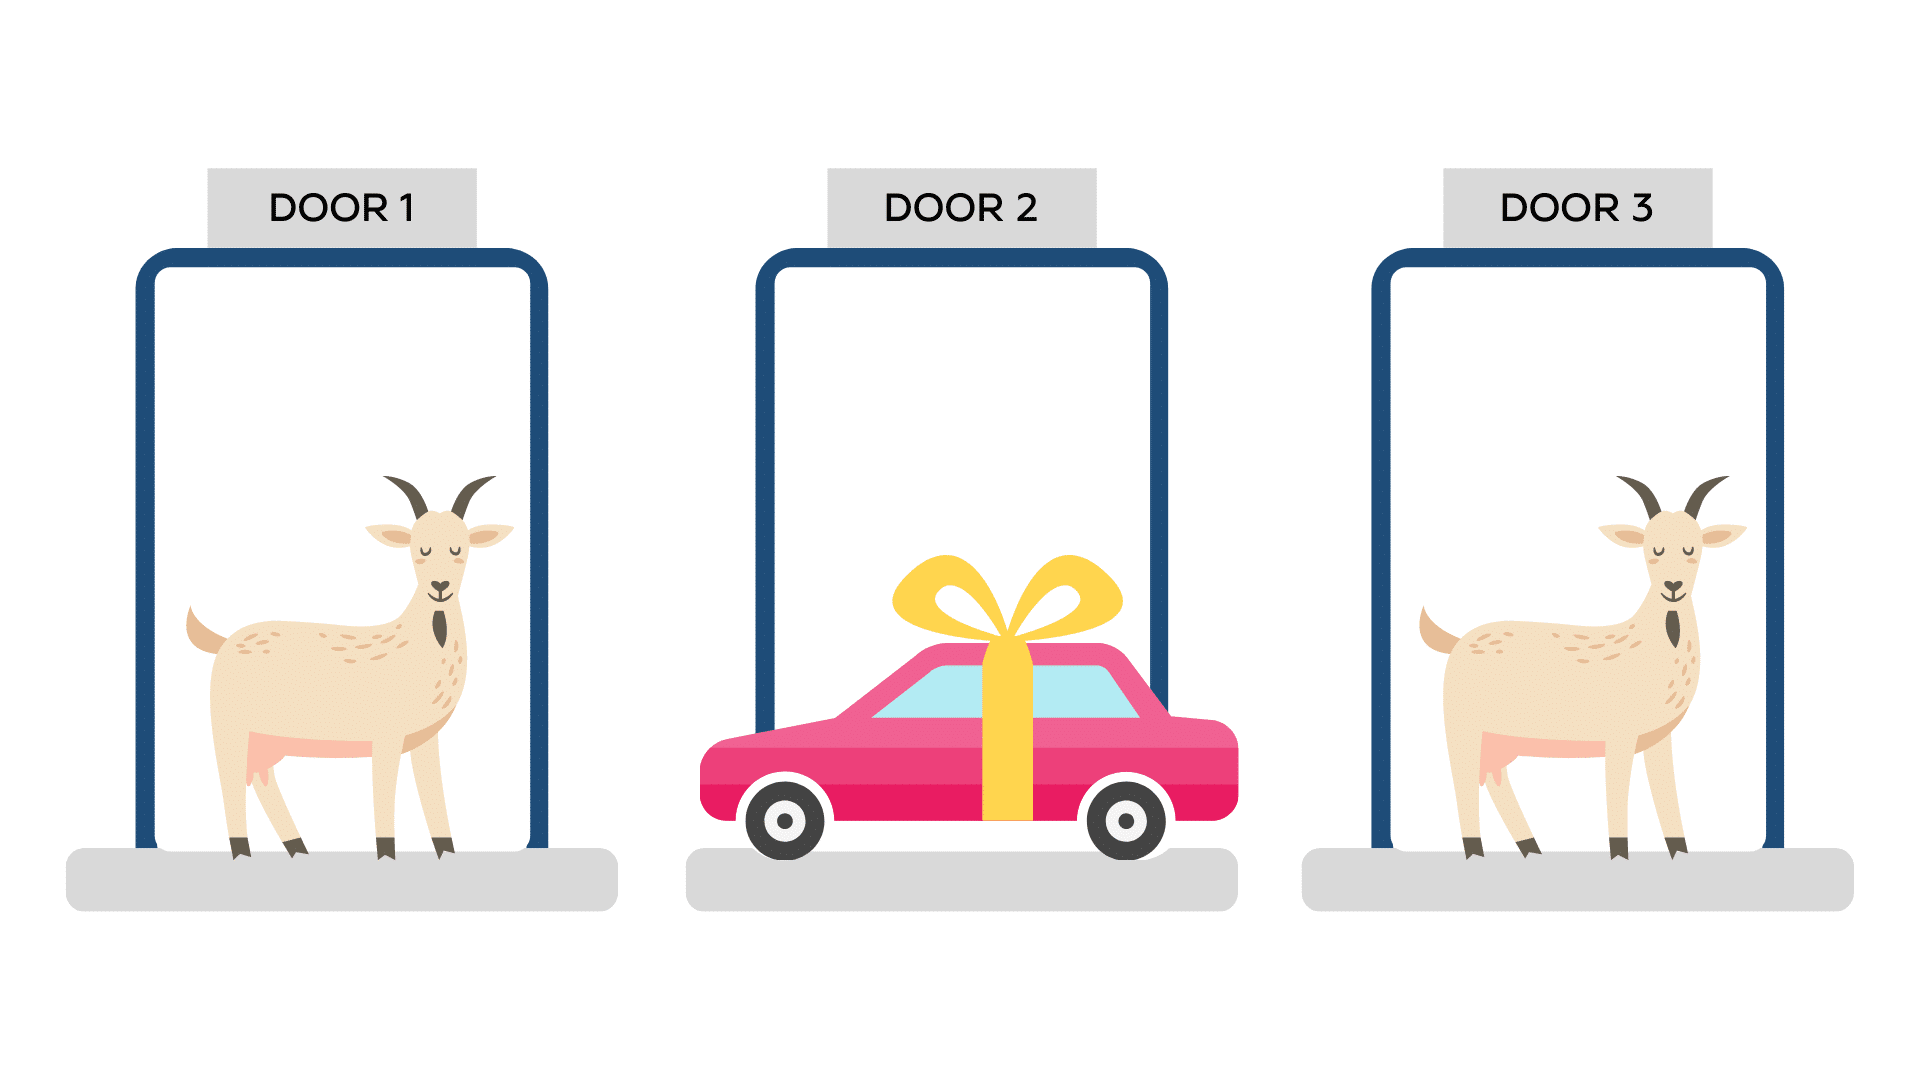
\includegraphics[scale=0.25]{MontyHall.png}  
\end{center}
\end{titlepage}
\nopagecolor
\tableofcontents
\chapter{Preliminari}
\section{Somme Infinite}
In questa sezione delineeremo il concetto di somma infinita, estendendo la nozione di serie, che useremo più avanti nello svilupparsi della teoria del Calcolo delle Probabilità.
\begin{myobs}
Supponiamo di avere un insieme $X$ non vuoto, ed una funzione $f:X\longrightarrow [0,+\infty)$. Se $X$ é finito, è chiaramente possibile dare un senso alla scrittura $\sum_{x\in X} f(x)$: basterebbe infatti ordinare $X = \{x_1,\dots,x_n\}$, e poi effettuare la somma $f(x_1)+\cdots+f(x_n)$, e definire $\sum_{x\in X} f(x)$ come uguale a tale somma. Questa sarebbe una definizione ben posta perché l'addizione di numeri reali è commutativa, e quindi non importa l'ordinamento di $X$ che usiamo per il calcolo di $\sum_{x\in X} f(x)$.\\
E se invece $X$ fosse numerabile? come possiamo dare un senso ad $\sum_{x\in X} f(x)$?.\\
Si potrebbe ritentare la stessa strategia, che quindi consisterebbe nell'ordinare $X = \{x_1,x_2,\dots\}$ e poi definire $\sum_{x\in X} f(x)$ come la serie $\sum_{n = 1}^\infty f(x_n)$.\\
Questa volta è più difficile mostrare che questa definizione non dipende dall'ordinamento, ma si può fare (vedi \cite{acerbibuttazzo})
\end{myobs}
Ora daremo la definizione che estenderà il concetto di serie.
\begin{boxdef}{Somma generalizzata}
\begin{mydef}
Sia $X$ un insieme non vuoto, ed $f:X \longrightarrow [0,+\infty)$ una funzione. Definiamo la somma generalizzata della famiglia $\{f(x)\}_{x\in X}$ nel seguente modo:
$$
\sum_{x\in X} f(x) := \sup\left\{\sum_{x\in A} f(x):\ A\subseteq X,\ A\textup{ finito}\right\}\in [0,+\infty].
$$
\end{mydef}
\end{boxdef}
\noindent
Di questa nozione di somma infinita si possono dimostrare una serie di fatti, tra cui il seguente:
\begin{boxpro}\label{pro:SommeGeneralizzateSommaFinita}
\begin{mypropo}
Sia $X$ un insieme, ed $f:X \longrightarrow [0,+\infty)$ una funzione. Allora se $\sum_{x\in X} f(x)$ è finito, risulta che l'insieme $\{x\in X:\ f(x) \neq 0\}$ è al più numerabile.
\end{mypropo}
\tcblower
\begin{proof}
Definiamo per ogni intero positivo $n$ l'insieme $X_n = \{x\in X:\ f(x) > n^{-1}\}$. Nota che:
$$
\{x\in X:\ f(x) \neq 0\} = \{x\in X:\ f(x) > 0\} = \bigcup_{n = 1}^\infty X_n.
$$
Se l'insieme in questione fosse più che numerabile, allora dovrebbe esistere qualche $X_n$ più che numerabile, e quindi conterrebbe un'infinità numerabile di elementi $\{x_1,x_2,\dots\}\subseteq X_n$, ma allora per ogni naturale $N \geq 1$ si avrebbe che:
$$
\sum_{x\in \{x_1,\dots,x_N\}} f(x) = \sum_{k = 1}^N f(x_k) > \sum_{k = 1}^N \frac{1}{n} = \frac{N}{n},
$$
cosa che renderebbe l'insieme:
$$
\left\{\sum_{x\in A} f(x) :\ A\subseteq X,\ A\textup{ finito}\right\}
$$
superiormente illimitato.
\end{proof}
\end{boxpro}
\noindent
Tra le altre cose che si riescono a dimostrare c'è il seguente fatto.
\begin{boxpro}
\begin{mypropo}\label{pro:SommeGeneralizzateIndipendenzaOrdinamento}
Sia $X$ un insieme non vuoto numerabile, ed $f:X\longrightarrow [0,+\infty)$ una funzione. Allora per qualsiasi biezione $g:\N \longrightarrow X$ si ha che:
$$
\sum_{x\in X} f(x) = \sum_{n = 1}^\infty f(g(n)).
$$
\end{mypropo}
\tcblower
\begin{proof}
Definiamo per ogni intero positivo $n$ l'insieme $B_n:= g(\{1,\dots,n\})\subseteq X$. Per ogni $F\subseteq X$ finito esiste un $B_n$ con $F \subseteq B_n$, dunque:
$$
\sum_{x\in F} f(x) \leq \sum_{x\in B_n} f(x) = \sum_{k = 1}^n f(x) \leq \sum_{x\in X} f(x).
$$
Siccome $\sum_{x\in B_n} f(x) \leq \sum_{x\in X} f(x)$, avremo $\sup_{n \geq 1} \sum_{x\in B_n} f(x) \leq \sum_{x\in X} f(x)$. D'altra parte $\sum_{x\in F} f(x) \leq \sum_{x\in B_n} f(x) \leq \sup_{n \geq 1} \sum_{x\in B_n} f(x)$, perciò:
$$
\sum_{x\in F} f(x) \leq \sup_{n \geq 1} \sum_{k = 1}^n f(x) = \sum_{k = 1}^\infty f(x) \leq \sum_{x\in X} f(x),
$$
ma siccome tale disuguaglianza vale per ogni sottoinsieme $F\subseteq X$ finito, avremo:
$$
\sum_{x\in X} f(x) = \sup\left\{\sum_{x\in F} f(x):\ F\subseteq X,\ F\textup{ finito}\right\}\leq \sum_{k = 1}^\infty f(x) \leq \sum_{x\in X} f(x).
$$
\end{proof}
\end{boxpro}
\noindent
Questo risponde alla domanda che ci siamo fatti all'incipit della sezione. Ci sono altre proprietà che questo tipo di somme infinite soddisfano.
\begin{boxpro}
\begin{mypropo}
Sia $X$ un insieme non vuoto, $f,g:X \longrightarrow [0,+\infty)$ due funzioni. Allora:
\begin{itemize}
\item[$(i)$] Dati $\alpha,\beta\in [0,+\infty)$ si ha:
$$
\sum_{x\in X} [\alpha f(x) + \beta g(x)] = \alpha \sum_{x\in X} f(x) + \beta \sum_{x\in X} g(x).
$$
\item[$(ii)$] Se per ogni $x\in X$ vale $f(x) \leq g(x)$, allora:
$$
\sum_{x\in X} f(x) \leq \sum_{x\in X} g(x).
$$
\item[$(iii)$] Data la famiglia $\{I_j\}_{j\in J}\subseteq \parti{X}$ di insiemi disgiunti con unione $X$, si ha:
$$
\sum_{x\in X} f(x) = \sum_{j\in J} \sum_{x\in I_j} f(x).
$$
\end{itemize}
\end{mypropo}
\end{boxpro}
\section{Teoria della Misura}
\subsection{Classe Monotona}
In questa sezione richiamo alcune nozioni e particolarità di teoria della misura che vedremo nel corso.\\
In primo luogo dobbiamo dare una definizione diversa da quella vista in TdM, la classe monotona.
\begin{boxdef}{Classe Monotona}
\begin{mydef}
Dato l'insieme non vuoto $X$, si dice classe monotona una qualsiasi famiglia $\mathcal{C}\subseteq \parti{X}$ tale che:
\begin{itemize}
\item[$(i)$] $X\in \mathcal{C}$.
\item[$(ii)$] Per ogni $A,B\in \mathcal{C}$ con $A\subseteq B$, si ha $B\tolto A \in \mathcal{C}$.
\item[$(iii)$] Per ogni $\{A_n\}_{n = 1}^\infty \subseteq \mathcal{C}$ ascendente si ha che:
$$
\bigcup_{n = 1}^\infty A_n \in \mathcal{C}.
$$
\end{itemize}
\end{mydef}
\end{boxdef}
\noindent
Notando che l'intersezione di classi monotone è ancora una classe monotona, partendo da una famiglia $\mathcal{E}\subseteq X$, si definisce la classe monotona generata da $\mathcal{E}$ coma la famiglia:
$$
\mathcal{C}(\mathcal{E}):= \bigcap \{\mathcal{C}:\ \mathcal{C}\textup{ è una classe monotona}, \ \mathcal{E}\subseteq \mathcal{C}\}.
$$
Con questa nozione di classe monotona vale una versione più forte del lemma della classe monotona a noi conosciuto da TdM.
\begin{boxoss}
\begin{mylem}
Sia $X$ un insieme non vuoto, ed $\mathcal{E}\subseteq \parti{X}$ una famiglia di sottoinsiemi di $X$ chiusa per intersezioni finite. Allora $\sigma(\mathcal{E}) = \mathcal{C}(\mathcal{E})$.
\end{mylem}
\end{boxoss}
\noindent
Questa nozione di classe monotona dà molta rilevanza alle famiglie chiuse per intersezioni finite, ed infatti data una $\sigma$-algebra $\mathcal{M}$, si dice base per $\mathcal{M}$ una qualsiasi famiglia $\mathcal{E}\subseteq \parti{X}$ chiusa per intersezioni finite con $\sigma(\mathcal{E}) = \mathcal{M}$.\\
Si ha il seguente teorema:
\begin{boxteo}{}
\begin{myteo}\label{teo:MisureFiniteUgualiSuBaseAlloraUgualiOvunque}
Sia $(X,\mathcal{M})$ uno spazio misurabile, $\mathcal{E}$ una base per $\mathcal{M}$, e siano $\mu$ e $\nu$ due misure finite su $(X,\mathcal{M})$ con $\mu(X) = \nu(X)$ che coincidono su $\mathcal{E}$. Allora $\mu = \nu$.
\end{myteo}
\tcblower
\begin{proof}
È chiaro che la famiglia $\mathcal{C}:= \{A\in \mathcal{M}:\ \mu(A) = \nu(A)\}$ è una classe monotona, e siccome questa contiene $\mathcal{E}$, abbiamo che $\mathcal{C}(\mathcal{E}) \subseteq \mathcal{C}$; ma per il lemma della classe monotona abbiamo che $\mathcal{C}(\mathcal{E}) = \sigma(\mathcal{E}) = \mathcal{M}$, e quindi $\mathcal{M} \subseteq \mathcal{C}$, che è un altro modo per affermare la tesi.
\end{proof}
\end{boxteo}
\begin{myes}
Una possibile base per $\mathcal{B}(\R^n)$ è la famiglia $\{(-\infty,\gri{x}]:\ \gri{x}\in \R^n\}$, dove per ogni $\gri{x}\in \R^n$ si definisce:
$$
(-\infty,\gri{x}] = (-\infty,x_1]\times \cdots \times (-\infty,x_n].
$$
Il fatto che tale famiglia genera $\mathcal{B}(\R^n)$ lo diamo per buono, mostriamo piuttosto che è chiusa per intersezioni finite: Dati $\gri{x},\gri{y}\in \R^n$:
$$
(-\infty,\gri{x}]\cap (-\infty,\gri{y}] = (-\infty,\min\{x_1,y_1\}]\times \cdots \times (-\infty,\min\{x_n,y_n\}],
$$
dove chiamando $\gri{z}\in \R^n$ il vettore di entrata $i$-esima $z_i := \min\{x_i,y_i\}$, otteniamo $(-\infty,\gri{x}]\cap (-\infty,\gri{y}] = (-\infty,\gri{z}]$.
\end{myes}
Questa famiglia ci servirà più in avanti.
\chapter{Introduzione}
\section{Che cos'è la probabilità}
La probabilità è qualcosa con cui tutti noi abbiamo avuto a che fare in un modo o nell'altro nelle nostre vite. Ora è giunto il momento di costruire una teoria matematica della probabilità.\\
In primo luogo, essa riguarda i cosiddetti esperimenti aleatori, ossia i fenomeni (situazioni del mondo reale) il cui esito non può essere previsto con certezza a priori (ossia prima vedere lo svolgimento di tale fenomeno).
In poche parole, la probabilità è la matematica degli esperimenti aleatori.\\
Come facciamo a costruire un modello della probabilità di un dato esperimento aleatorio?\\
Ci sono tre componenti fondamentali.
\subsection{Spazio Campionario}
Lo spazio campionario è l'insieme (inteso in senso matematico) di tutti i possibili esiti dell'esperimento, tipicamente indicato con $\Omega$.
\begin{myes}\label{es:EsempioSpazioCampionarioABC}\hfill
\begin{itemize}
\item[$(a)$] Se stiamo studiando il lancio di un dado a $6$ facce, lo spazio campionario è $\Omega = \{1,2,3,4,5,6\}$, dove con ciascun numero indichiamo appunto l'esito del lancio.
\item[$(b)$] Se stiamo studiando il risultato delle elezioni, ed in particolare il numero di voti ottenuti da un certo politico "Cetto", possiamo prendere come spazio campionario l'insieme $\Omega = \{0,1,\dots,M\}$, dove $M$ è il numero di aventi diritto al voto.\\
Potremmo anche aver preso $\Omega = \N_0$, in genere non c'è nulla di male nel prendere un insieme che contenga più eventi di quelli possibili.
\item[$(c)$] Se stiamo studiando il tempo di emissione di una particella radioattiva, possiamo modellare l'insieme di tutti gli esiti prendendo $\Omega = [0,+\infty)$.
\end{itemize}
\end{myes}
La richiesta di partire con un insieme $\Omega$ che contenga tutti gli eventi possibili.
\subsection{Eventi}
Una cosa necessaria per poter studiare la probabilità di un fenomeno aleatorio è la descrizione degli eventi. Un evento da intendere come un'affermazione sull'esito dell'esperimento aleatorio in questione, e può essere interpretato matematicamente come un sottoinsieme dello spazio campionario, secondo la seguente corrispondenza:
$$
\textup{"L'esito soddisfa la proprietà x"}\quad \iff \quad \{a\in \Omega:\ a\textup{ soddisfa x}\}
$$
\begin{myes}\hfill
\begin{itemize}
\item[$(a)$] L'affermazione "esce un numero pari" corrisponde all'insieme $A = \{2,4,6\}$; l'affermazione "esce un numero multiplo di $3$" corrisponde invece all'insieme $B = \{3,6\}$; mentre l'affermazione "esce il numero $6$" corrisponde all'insieme $C = \{6\}$.\\
Nota che $C = A\cap B$, e che l'affermazione "esce il numero $6$" equivale a dire "esce un numero pari ed esce un multiplo di 3".
\item[$(b)$] L'affermazione "Cetto non ottiene alcun voto" corrisponde all'insieme $D = \{0\}$, mentre, prendendo $\Omega = \{0,1,\dots,M\}$, l'affermazione "Cetto ottiene $M+1$ voti" corrisponde all'insieme $E = \varnothing$, siccome non c'è alcun evento in $\Omega$ per cui valga tale affermazione.\\
Naturalmente prendendo $\Omega = \N_0$, avremmo $E = \{M+1\}$.
\item[$(c)$] L'affermazione "la particella è emessa dopo 3 mesi", misurando il tempo in secondi, corrisponde all'insieme $F = (3\cdot 30 \cdot 24 \cdot 60 \cdot 60, +\infty)$.
\end{itemize}
\end{myes}
La domanda che ci facciamo ora è la seguente: "È sensato prendere come eventi tutti i sottoinsiemi dello spazio campionario?".\\
La realtà è che dipende. Se $\Omega$ è al più numerabile (come negli esempi $(a)$ e $(b)$), allora lo si può senz'altro fare, ciò vale a dire che, se $\mathcal{A}$ è la famiglia di tutti gli eventi, possiamo prendere $\mathcal{A} = \parti{\Omega}$.\\
Se invece $\Omega$ è più che numerabile (come nel caso dell'esempio $(c)$), allora è opportuno, per ragioni tecniche, considerare come eventi solo alcuni tra i sottoinsiemi di $\Omega$, in altre parole, è opportuno prendere $\mathcal{A}\subset \parti{X}$.
In particolare, è naturale assumere le seguenti proprietà:
\begin{itemize}
\item $\varnothing \in \mathcal{A}$.
\item Se $A\in \mathcal{A}$, allora $A^c = \Omega \tolto A \in \mathcal{A}$.\\
Se possiamo dire qualcosa sull'esito dell'evento, allora possiamo dire anche il suo opposto.
\item Se $A,B\in \mathcal{A}$, allora $A\cup B\in \mathcal{A}$.\\
Se possiamo affermare due cose sull'evento, allora possiamo affermare che l'esito soddisfi almeno una delle due.
\end{itemize}
La prima proprietà potrebbe sembrare strana, ed infatti è richiesta per questioni di vacuità, ma equivalentemente si potrebbe richiedere che $\mathcal{A}$ non sia vuota (dalle altre proprietà si otterrebbe che $\varnothing\in \mathcal{A}$).\\
Queste tre proprietà descrivono una categoria di famiglie particolare, chiamate Algebre.\\
In realtà, però, cercando di costruire la teoria prendendo $\mathcal{A}$ come un'Algebra, si scopre che non è abbastanza, in particolare quando si trattano i limiti. Quello che aggiusterà questa mancanza sarà la richiesta di avere $\mathcal{A}$ come una $\sigma$-Algebra, ossia una famiglia non vuota tale che:
\begin{itemize}
\item Se $A\in \mathcal{A}$, allora $A^c\in \mathcal{A}$.
\item Se $\{A_n\}_{n = 1}^\infty \subseteq \mathcal{A}$, allora l'unione $\bigcup_{n = 1}^\infty A_n \in \mathcal{A}$.
\end{itemize}
\subsection{Probabilità}
La probabilità è un "grado di fiducia" che si associa al verificarsi di un evento $A\in \mathcal{A}$, espresso con un numero in $[0,1]$ (o equivalentemente una percentuale).\\
In altre parole si tratta di una funzione $\P:\mathcal{A}\longrightarrow [0,1]$.\\
Ma che cosa vuol dire grado di fiducia? Esistono diverse interpretazioni, tra cui presentiamo le due seguenti
\begin{itemize}
\item Interpretazione Frequentista\\
Supponendo di poter ripetere l'esperimento nelle stesse condizioni un numero elevato $N >> 1$ di volte. Dato un evento $A\in \mathcal{A}$, possiamo contare il numero di volte in cui si verifica l'evento $A$, indicando tale numero con $\mathcal{C}_N(A)$. Allora si otterrà che la probabilità dell'evento $A$, $\P(A)$ sarà all'incirca uguale a $\mathcal{C}_N(A)/N$.
\item Interpretazione Soggettivista\\
La probabilità di un evento $A$ rappresenta il "prezzo equo" di una scommessa che paga 1 se si verifica $A$, e $0$ altrimenti.\\
Per esempio, se un evento ha probabilità $0.5$, affinché io trovi vantaggioso il partecipare alla scommessa, il prezzo per partecipare dovrà essere minore di $0.5$, ed affinché trovi vantaggioso giocare come il banco, il prezzo per partecipare dovrà essere maggiore di $0.5$.
\end{itemize}
Ora, la funzione $\P:\mathcal{A}\longrightarrow [0,1]$, è chiaro che non potrà essere una funzione qualsiasi, e che dovrà soddisfare alcune proprietà. Queste proprietà le possiamo intuire dall'interpretazione frequentista.
\begin{itemize}
\item[$(i)$] $\P(\varnothing) = 0$.\\
Questo lo si deduce dal fatto che per ogni $N$, $\mathcal{C}_N(\varnothing) = 0$.
\item[$(ii)'$] Se $A,B\in \mathcal{A}$ sono tali che $A \cap B = \varnothing$, allora $\P(A\cup B) = \P(A)+\P(B)$.\\
Questo lo si deduce dal fatto che se $A$ e $B$ sono disgiunti, allora evidentemente $\mathcal{C}_N(A\cup B) = \mathcal{C}_N(A)+\mathcal{C}_N(B)$ vale per ogni $N$.
\end{itemize}
Anche qui, cercando di costruire la teoria con queste richieste per la probabilità non da' risultati del tutto soddisfacenti, ed in merito al secondo punto si tende a chiedere di più, in particolare:
\begin{itemize}
\item[$(ii)$] Se $\{A_n\}_{n = 1}^\infty\subseteq \mathcal{A}$ è tale che $A_i \cap A_j = \varnothing$ per ogni $i \neq j$, allora: $$
\P\Bigg(\bigcup_{n = 1}^\infty A_n\Bigg) = \sum_{n = 1}^\infty \P(A_n).
$$
\end{itemize}
Arriviamo quindi agli assiomi di probabilità.
\section{Assiomi di probatilità}
\subsection{Definizione, esempi, e proprietà}
\begin{boxdef}{Spazio di probabilità}
\begin{mydef}
Si chiama spazio delle probabilità una qualsiasi terna $(\Omega,\mathcal{A},\P)$, dove:
\begin{itemize}
\item $\Omega$ è un insieme non vuoto.
\item $\mathcal{A}\subseteq \parti{\Omega}$ è una $\sigma$-Algebra.
\item $\P:\mathcal{A}\longrightarrow [0,1]$ è una probatilità, ossia una funzione soddisfacente:
\begin{itemize}
\item[\textup{(P1)}] $\P(\Omega) = 1$.
\item[\textup{(P2)}] Per ogni $\{A_n\}_{n = 1}^\infty\subseteq \mathcal{A}$, famiglia numerabile di insiemi disgiunti, risulta:
$$
\P\Bigg(\bigcup_{n = 1}^\infty A_n\Bigg) = \sum_{n = 1}^\infty \P(A_n). 
$$
\end{itemize}
\end{itemize}
\end{mydef}
\end{boxdef}
\begin{mynota}
L'assioma (P1) è effettivamente diverso da quello che avevo preannunciato, ossia $\P(\varnothing) = 0$; vedremo più avanti come questa è una cosa che si deduce da (P1) e (P2), ma dal punto di vista storico si è scelto (P1), ed è effettivamente più comodo per costruire la teoria.
\end{mynota}
\begin{mynota}
Da qui in avanti, quando $\Omega$ sarà finito o numerabile, daremo per scontato che $\mathcal{A} = \parti{X}$, mentre nel caso in cui $\Omega$ sia $\R^n$ allora sceglieremo sempre la $\sigma$-Algebra di Borel.
\end{mynota}
\begin{boxpro}
\begin{mypropo}
Sia $(\Omega,\mathcal{A},\P)$ uno spazio di probabilità, allora:
\begin{itemize}
\item[$(i)$] $\P(\varnothing) = 0$.
\item[$(ii)$] Dati $A_1,\dots,A_N\in \mathcal{A}$ disgiunti a due a due, risulta:
$$
\P\Bigg(\bigcup_{k = 1}^N A_k\Bigg) = \sum_{k = 1}^N \P(A_k).
$$
\end{itemize}
\end{mypropo}
\tcblower
\begin{proof}
\hfill
\begin{flushleft}
$(i)$
\end{flushleft}
Consideriamo $\{A_n\}_{n = 1}^\infty \subseteq \mathcal{A}$, data da $A_n = \varnothing$ per ogni $n\geq 1$. Evidentemente $A_n \cap A_m = \varnothing$ per ogni $n\neq m$, dunque ci è lecito usare la $\sigma$-Additività:
$$
\P(\varnothing) = \P\Bigg(\bigcup_{n = 1}^\infty A_n\Bigg) = \sum_{n = 1}^\infty \P(A_n) = \sum_{n = 1}^\infty \P(\varnothing),
$$
ed essendo $\P(\varnothing) = \sum_{n = 1}^\infty \P(\varnothing)$ un numero reale compreso tra $0$ e $1$, deve essere che $\P(\varnothing) = 0$: altrimenti la serie sarebbe $+\infty$.
\begin{flushleft}
$(ii)$
\end{flushleft}
Consideriamo $\{B_n\}_{n = 1}^\infty \subseteq \mathcal{A}$ data da:
$$
B_n = \begin{cases}
A_n &\textup{ se }1\leq n \leq N,\\
\varnothing &\textup{ se }n>N.
\end{cases}
$$
È evidente che $B_n \cap B_m = \varnothing$ per ogni $n\neq m$, dunque:
\begin{align*}
\P\Bigg(\bigcup_{k = 1}^N A_k\Bigg) &= \P\Bigg(\bigcup_{k = 1}^\infty B_k\Bigg) = \sum_{k = 1}^\infty \P(B_k) = \sum_{k = 1}^N \P(B_k) + \sum_{k = N+1}^\infty \P(B_k) = \sum_{k = 1}^N \P(A_k) + \sum_{k = N+1}^\infty \P(\varnothing)\\
&= \sum_{k = 1}^N \P(A_k).
\end{align*}
\end{proof}
\end{boxpro}
\begin{myobs}
La finita additività non implica la $\sigma$-additività. Seppur questo fatto possa sembrare ragionevole, esibire un controesempio non è poco impegnativo.
\end{myobs}
\begin{myobs}
Con un ragionamento per induzione si dimostra che dire che $\P$ è finitamente additiva vuol dire che per ogni $A,B\in \mathcal{A}$ disgiunti, risulta $\P(A\cup B) = \P(A)+\P(B)$.
\end{myobs}
\begin{myobs}
Questa proposizione illustra il legame (già intuibile dagli assiomi di probabilità) che c'è tra la teoria della misura e il calcolo delle probabilità.\\
Infatti ogni spazio di probabilità è una misura, ed in particolare, gli spazi di probabilità sono tutti e soli gli spazi di misura con misura avente massa $1$ (la massa di una misura $\mu$ è semplicemente il valore che assume su tutto lo spazio).\\
Inoltre, vale anche la pena notare a questo punto che se $(\Omega,\mathcal{A},\mu)$ è uno spazio di misura con massa finita e non nulla, allora la funzione $\P:\mathcal{A}\longrightarrow [0,1]$ data da:
$$
\P(A) = \frac{\mu(A)}{\mu(\Omega)},
$$
è una probabilità su $(\Omega,\mathcal{A})$.
\end{myobs}
\begin{mynota}
Approfitto della parentesi fatta a teoria della misura che viene chiamato supporto di una misura $\mu$ su $(\Omega,\mathcal{A})$ un qualsiasi sottoinsieme $\widetilde{\Omega}\in \mathcal{A}$ per cui $\mu(\widetilde{\Omega}^c) = 0$.
\end{mynota}
\begin{myes}
Con le conoscenze di teoria della misura siamo in grado di fornire un esempio di spazio di probabilità. Considera $\Omega = [0,1]$, $\mathcal{A} = \Borel([0,1])$ come la famiglia dei Boreliani di $[0,1]$, e $\P = m:\Borel([0,1])\longrightarrow [0,1]$ la misura di Lebesgue ristretta all'intervallo $[0,1]$.\\
Essendo questo uno spazio di misura con massa $1$, abbiamo il nostro primo esempio di spazio di probabilità.\\
L'esperimento aleatorio che questo spazio potrebbe descrivere è per esempio l'estrazione casuale di un numero reale tra $0$ e $1$.
\end{myes}
Costruire la misura di Lebesgue è molto complicato, e questo esempio potrebbe non essere molto soddisfacente.\\
Presentiamo ora uno degli esempi di spazio di probabilità che ci accompagnerà fino alla fine.
\begin{myes}
Sia $\Omega$ un insieme finito e non vuoto di cardinalità $N$. Definiamo $\P:\parti{\Omega}\longrightarrow [0,1]$ ponendo:
$$
\P(A) = \frac{|A|}{|\Omega|} = \frac{|A|}{N},
$$
e verifichiamo che si tratta di una probabilità.\\
(P1) è facile da dimostrare, siccome $\P(\Omega) = N/N = 1$. Dedichiamoci a (P2).\\
Prendiamo una qualsiasi famiglia numerabile di sottoinsiemi disgiunti di $\Omega$, $\{A_n\}_{n = 1}^\infty \subseteq \parti{\Omega}$, chiamando $A$ la loro unione. Siccome $A\subseteq \Omega$ e tale insieme è finito, deve accadere che $A$ è finito, e quindi non può accadere che ci sono infiniti $A_n$ non vuoti (altrimenti, essendo questi disgiunti, avremmo $A$ infinito), e perciò deve esistere un indice $m\geq 1$ per la quale $A_n = \varnothing$ per ogni $n>m$, ma allora:
$$
\P\Bigg(\bigcup_{n = 1}^\infty A_n\Bigg) = \P\Bigg(\bigcup_{n = 1}^m A_n\Bigg) = \frac{1}{N}\Bigg|\bigcup_{n = 1}^m A_n\Bigg| = \frac{1}{N}\sum_{n = 1}^m |A_n| = \sum_{n = 1}^m \P(A_n) = \sum_{n = 1}^\infty \P(A_n)
$$
(gli $A_n$ sono disgiunti a due a due, dunque la cardinalità dell'unione è semplicemente la somma delle cardinalità dei singoli insiemi).\\
Questa probabilità viene chiamata probabilità uniforme discreta, ed è l'unica probabilità su $\Omega$ per cui tutti gli esiti sono equiprobabili (vale a dire che $\P$ è costante sui singoletti).\\
Nell'esempio (\ref{es:EsempioSpazioCampionarioABC}), in particolare in $(a)$, un ottima scelta della probabilità, dato $\Omega = \{1,2,3,4,5,6\}$, è proprio la probabilità uniforme discreta, in quanto per un dado regolare non c'è nessun motivo per cui una faccia debba uscire più spesso delle altre.
\end{myes}
\begin{myes}\label{es:EsempioCarteIdentitàPt1}
Supponiamo di avere un gruppo di $n > 1$ persone, e come esperimento aleatorio immaginiamo di prendere la carta d'identità di ciascuna di esse, ridistribuendole casualmente. In primo luogo va scelto uno spazio campionario: per farlo bisogna decodificare gli esiti. Che cos'è un esito in questo contesto? Identificando ciascuna persona con un numero da $1$ a $n$, un esito dell'esperimento è possibile vederlo come un insieme di coppie in $\{1,\dots,n\}\times \{1,\dots,n\}$ le cui prime entrate rappresenta il numero della persona e in questione, e la seconda entrata rappresenta il numero della persona di cui ha ricevuto la carta d'identità. Questo insieme deve avere delle proprietà:
\begin{itemize}
\item Tutti ricevono una carta d'identità, quindi per ogni $k\in \{1,\dots,n\}$, ci deve essere una coppia del tipo $(k,j)$.
\item Ciascuno riceve una carta d'identità, quindi tale insieme non può contenere coppie con numeri diversi in seconda entrata, e al contempo lo stesso numero come prima entrata.
\item Le carte d'identità sono uniche, quindi tale insieme non può contenere coppie con prima entrata diversa e seconda entrata uguali.
\item Vengono ridistribuite tutte le carte d'identità, quindi per ogni $j\in \{1,\dots,n\}$, ci deve essere una coppia del tipo $(k,j)$.
\end{itemize}
Un sottoinsieme di $\{1,\dots,n\}\times \{1,\dots,n\}$ è anche conosciuto sotto il nome di relazione su $\{1,\dots,n\}$, ed in particolare, i primi due punti ci permettono di dire che tale relazione è una funzione, ed i secondi due ci dicono che tale funzione deve essere biettiva, dunque prendiamo come insieme degli eventi il seguente:
$$
\Omega = \{\sigma:\{1,\dots,n\}\longrightarrow \{1,\dots,n\}:\ \sigma \textup{ è biettiva}\},
$$
che è anche conosciuto sotto il nome di gruppo simmetrico di ordine $n$, indicato con $\Sym{n}$.\\
Considerando la probabilità uniforme, $\P:\parti{\Omega}\longrightarrow [0,1]$, dal momento che $|\Omega| = |\Sym{n}| = n!$, avremo che per ogni $A\subseteq \Omega$ risulta:
$$
\P(A) = \frac{|A|}{n!}.
$$
In questo linguaggio, l'affermazione "nessuno riceve la propria carta d'identità" corrisponde all'insieme:
$$
A = \{\sigma\in \Sym{n}:\ \forall i\in \{1,\dots,n\},\ \sigma(i) \neq i\}.
$$
In un esempio futuro vedremo come calcolare la cardinalità di questo insieme.
\end{myes}
\begin{boxpro}
\begin{mypropo}\label{pro:ProprietàSempliciProbabilità}
Sia $(\Omega,\mathcal{A},\P)$ uno spazio di probabilità. Allora:
\begin{itemize}
\item[$(i)$] Dati gli eventi $A,B\in \mathcal{A}$ con $A\subseteq B$ risulta $\P(B\tolto A) = \P(B)-\P(A)$, ed in particolare $\P(A)\leq \P(B)$.
\item[$(ii)$] Per ogni evento $A\in \mathcal{A}$ si ha $\P(A^c) = 1-\P(A)$.
\item[$(iii)$] Dati gli eventi $A,B\in \mathcal{A}$, risulta:
$$
\P(A\cup B) = \P(A)+\P(B) - \P(A\cap B),
$$
ed in particolare $\P(A\cup B) \leq \P(A) + \P(B)$.
\end{itemize}
\end{mypropo}
\tcblower
\begin{proof}
\hfill
\begin{flushleft}
$(i)$
\end{flushleft}
Osserva che $B = A \cup B\tolto A$ è un'unione disgiunta, quindi in virtù dell'additività finita avremo che $\P(B) = \P(A)+ \P(B\tolto A)$, e perciò portando $\P(A)$ dall'altro lato dell'uguaglianza risulterà che $\P(B\tolto A) = \P(B) - \P(A)$. Da quest'uguaglianza si deduce che $\P(B) - \P(A)$ è maggiore uguale di $0$, essendo $\P(B\tolto A) \in [0,1]$, ergo $\P(A)\leq \P(B)$.
\begin{flushleft}
$(ii)$
\end{flushleft}
$A^c$ è per definizione uguale a $\Omega \tolto A$, ed essendo $A\subseteq \Omega$, deduciamo da $(i)$ che $\P(A^c) =  \P(\Omega\tolto A) = \P(\Omega) - \P(A) = 1-\P(A)$.
\begin{flushleft}
$(iii)$
\end{flushleft}
Osserva che $A\cup B = A \cup B \tolto A$ è un'unione disgiunta, dunque in virtù dell'additività finita risulterà che $\P(A\cup B) = \P(A) + \P(B\tolto A)$, e notando che $B \tolto A = B \tolto (A\cap B)$, essendo $A\cap B \subseteq B$ possiamo applicare $(i)$, deducendo che $\P(A\cup B) = \P(A) + \P(B\tolto(A\cap B)) = \P(A)+ \P(B) - \P(A\cap B)$.\\
Essendo $\P(A\cap B) \geq 0$ si ha chiaramente $\P(A\cup B) = \P(A) + \P(B) - \P(A\cap B) \leq \P(A) + \P(B)$.
\end{proof}
\end{boxpro}
\noindent 
Nota che nelle dimostrazioni di ciascuno di questi punti non abbiamo usato la $\sigma$-additività, ma solo l'additività finita.
\begin{myes}
Supponiamo di lanciare 8 volte un dado regolare a $6$ facce. Qual'è la probabilità che esca almeno un $6$?\\
Per prima cosa fissiamo lo spazio campionario. Un esito è codificabile con una lista ordinata di numeri da $1$ a $6$, dove la posizione del numero nella lista ordinata indica se si tratta del primo lancio, del secondo lancio, e via dicendo. Scegliamo quindi:
$$
\Omega:= \{1,\dots,6\}^8 = \{(\omega_1,\omega_2,\omega_3,\omega_4,\omega_5,\omega_6,\omega_7,\omega_8):\ \forall i\in \{1,\dots,8\},\ \omega_i\in \{1,\dots,6\}\}.
$$
Anche qui non c'è alcuna ragione di creda che ogni esito non sia equiprobabile, quindi scegliamo la probabilità uniforme discreta.\\
Per poter calcolare la probabilità di un evento ci servirà sapere la cardinalità di $\Omega$, che è $6^8$.
L'evento $A$ che ci interessa è rappresentato dal seguente insieme:
$$
A = \{(\omega_1,\omega_2,\omega_3,\omega_4,\omega_5,\omega_6,\omega_7,\omega_8):\ \exists i\in \{1,\dots,8\}:\ \omega_i = 6\}.
$$
Per trovare la probabilità di questo evento dobbiamo calcolare la cardinalità di $A$, che non è facile. Per risolvere il problema cerchiamo di trovare $\P(A^c) = 1-\P(A)$. Questo è molto conveniente dal momento che:
$$
A^c =  \{(\omega_1,\omega_2,\omega_3,\omega_4,\omega_5,\omega_6,\omega_7,\omega_8):\ \forall i\in \{1,\dots,8\}:\ \omega_i \neq 6\} = \{1,\dots,5\}^8,
$$
dunque evidentemente $|A^c| = 5^8$. Perciò:
$$
\P(A) = 1- \P(A^c) = 1 - \frac{5^8}{6^8} \approx 0.77.
$$
\end{myes}
Nella proposizione (\ref{pro:ProprietàSempliciProbabilità}) abbiamo visto che dati due eventi $A$ e $B$, risulta che $\P(A\cup B) = \P(A) +\P(B) -\P(A\cap B)$. Ma che cosa succede per l'unione finita di più di due insiemi?
\begin{myobs}
Siano $A,B,C$ tre eventi, cerchiamo di determinare $\P(A\cup B \cup C)$ in termini di altre probabilità. Abbiamo:
\begin{align*}
\P(A\cup B \cup C) &= \P((A\cup B)\cup C) = \P(A\cup B) + \P(C) - \P((A\cup B)\cap C)\\
&= \P(A\cup B) + \P(C) - \P((A\cap C)\cup (B\cap C))\\
&= \P(A)+\P(B)-\P(A\cap B) + \P(C) - \P(A\cap C)-\P(B\cap C) + \P((A\cap C)\cap (B \cap C)) \\
&= \P(A) + \P(B) + \P(C) - \P(A\cap B) - \P(A\cap C) - \P(B \cap C) + \P(A\cap B \cap C).
\end{align*}
Vista così questa formula è abbastanza scarna, cerchiamo di capirne il senso interpretando la probabilità di un evento come l'area di un insieme (d'altronde la probabilità è un particolare tipo di misura).\\
Come calcolerei $\P(A\cup B \cup C)$? Se i tre insiemi fossero disgiunti tale numero sarebbe $\P(A)+\P(B)+\P(C)$, ma nel caso generale saremmo in una situazione del genere:
\begin{center}
\begin{tikzpicture}[scale = 1.0]
    % Parametro di distanza di \Omega dal bordo
    \pgfmathsetmacro{\eps}{0.2}
    % \Omega
    \draw[thick] \rectangle;
    \node[] at ({-1.75+\eps},{-3.25+\eps}){$\Omega$};
    % Insieme A
    \draw \firstcircle;
    \node[left] at (-0.85,1.35){$A$};
    \fill[color = blue!66!black, fill opacity = 0.33] \firstcircle;
    % Insieme B
    \draw \secondcircle;
    \node[right] at (2.85,1.35){$B$};
    \fill[color =blue!66!black, fill opacity = 0.33] \secondcircle;
    % Insieme C
    \draw \thirdcircle;
    \node[right] at (2.0,-2.75){$C$};
    \fill[color = blue!66!black, fill opacity = 0.33] \thirdcircle;
    \node[below] at (1,-3.25){\scriptsize{$\P(A)+\P(B)+\P(C)$}};
\end{tikzpicture}
\end{center}
Vediamo che sommando le aree di $A$, $B$, e $C$, contiamo due volte le aree di $A\cap B$, $A\cap C$, e $B\cap C$, e contiamo tre volte l'area di $A\cap B \cap C$, dunque per aggiustare il tiro dobbiamo sottrarre l'area di $A\cap B$, $A\cap C$, e $B\cap C$:
\begin{center}
\begin{tikzpicture}[scale = 1.0]
    % Parametro di distanza di \Omega dal bordo
    \pgfmathsetmacro{\eps}{0.2}
    % \Omega
    \draw[thick] \rectangle;
    \node[] at ({-1.75+\eps},{-3.25+\eps}){$\Omega$};
    % Insieme A
    \draw \firstcircle;
    \node[left] at (-0.85,1.35){$A$};
    \fill[color = blue!66!black, fill opacity = 0.33] \firstcircle;
    % Insieme B
    \draw \secondcircle;
    \node[right] at (2.85,1.35){$B$};
    \fill[color =blue!66!black, fill opacity = 0.33] \secondcircle;
    % Insieme C
    \draw \thirdcircle;
    \node[right] at (2.0,-2.75){$C$};
    \fill[color = blue!66!black, fill opacity = 0.33] \thirdcircle;
    % Insieme A \cap B
    \begin{scope}
        \clip \firstcircle;
        \clip \secondcircle;
        \fill[white] \firstcircle;
        \fill[color = blue!66!black, fill opacity = 0.33] \secondcircle;
        \fill[white] \thirdcircle;
        \draw \firstcircle;
        \draw \secondcircle;
        \draw \thirdcircle;
    \end{scope}
    % Insieme B \cap C
    \begin{scope}
        \clip \secondcircle;
        \clip \thirdcircle;
        \fill[white] \secondcircle;
        \fill[color = blue!66!black, fill opacity = 0.33] \thirdcircle;
        \fill[white] \firstcircle;
        \draw \firstcircle;
        \draw \secondcircle;
        \draw \thirdcircle;
    \end{scope}
    % Insieme C \cap A
    \begin{scope}
        \clip \thirdcircle;
        \clip \firstcircle;
        \fill[white] \thirdcircle;
        \fill[color = blue!66!black, fill opacity = 0.33] \firstcircle;
        \fill[white] \secondcircle;
        \draw \firstcircle;
        \draw \secondcircle;
        \draw \thirdcircle;
    \end{scope}
    % Descrizione sotto
    \node[below] at (1,-3.25){\scriptsize{$\P(A)+\P(B)+\P(C)$}};
    \node[below] at (1,{-3.25-0.30}){\scriptsize{$-\P(A\cap B) - \P(A \cap C) - \P(B \cap C)$}};
\end{tikzpicture}
\end{center}
Tuttavia non abbiamo finito, perché in questo modo togliamo un'area di $A\cap B \cap C$ di troppo, che va quindi riaggiunta.
\begin{center}
\begin{tikzpicture}[scale = 1.0]
    % Parametro di distanza di \Omega dal bordo
    \pgfmathsetmacro{\eps}{0.2}
    % \Omega
    \draw[thick] \rectangle;
    \node[] at ({-1.75+\eps},{-3.25+\eps}){$\Omega$};
    % Insieme A
    \draw \firstcircle;
    \node[left] at (-0.85,1.35){$A$};
    \fill[color = blue!66!black, fill opacity = 0.33] \firstcircle;
    % Insieme B
    \draw \secondcircle;
    \node[right] at (2.85,1.35){$B$};
    \fill[color =blue!66!black, fill opacity = 0.33] \secondcircle;
    % Insieme C
    \draw \thirdcircle;
    \node[right] at (2.0,-2.75){$C$};
    \fill[color = blue!66!black, fill opacity = 0.33] \thirdcircle;
    % Insieme A \cap B
    \begin{scope}
        \clip \firstcircle;
        \clip \secondcircle;
        \fill[white] \firstcircle;
        \fill[color = blue!66!black, fill opacity = 0.33] \secondcircle;
        \fill[white] \thirdcircle;
        \draw \firstcircle;
        \draw \secondcircle;
        \draw \thirdcircle;
    \end{scope}
    % Insieme B \cap C
    \begin{scope}
        \clip \secondcircle;
        \clip \thirdcircle;
        \fill[white] \secondcircle;
        \fill[color = blue!66!black, fill opacity = 0.33] \thirdcircle;
        \fill[white] \firstcircle;
        \draw \firstcircle;
        \draw \secondcircle;
        \draw \thirdcircle;
    \end{scope}
    % Insieme C \cap A
    \begin{scope}
        \clip \thirdcircle;
        \clip \firstcircle;
        \fill[white] \thirdcircle;
        \fill[color = blue!66!black, fill opacity = 0.33] \firstcircle;
        \fill[white] \secondcircle;
        \draw \firstcircle;
        \draw \secondcircle;
        \draw \thirdcircle;
    \end{scope}
    % Insieme A \cap B \cap C
    \begin{scope}
        \clip \firstcircle;
        \clip \secondcircle;
        \clip \thirdcircle;
        \fill[color = blue!66!black, fill opacity = 0.33] \firstcircle;
        \draw \firstcircle;
        \draw \secondcircle;
        \draw \thirdcircle;
    \end{scope}
    % Descrizione sotto
    \node[below] at (1,-3.25){\scriptsize{$\P(A)+\P(B)+\P(C)$}};
    \node[below] at (1,{-3.25-0.30}){\scriptsize{$-\P(A\cap B) - \P(A \cap C) - \P(B \cap C)$}};
    \node[below] at (1,{-3.25-0.60}){\scriptsize{$+\P(A\cap B \cap C)$}};
\end{tikzpicture}
\end{center}
E se invece avessimo quattro insiemi $A$, $B$, $C$, e $D$? La procedura è la stessa, prima si sommano $\P(A)+\P(B)+\P(C)+\P(D)$, poi si sottraggono le probabilità delle intersezioni di coppie di insiemi, poi si risommano le probabilità delle intersezioni di terne di insiemi, ed infine si risottrae $\P(A\cap B\cap C \cap D)$.
\end{myobs}
Si può dimostrare una formula generale, ma come ci si può aspettare la formula è piuttosto brutta e incasinata. L'importante però è averne capito il senso.
\begin{boxteo}{Formula di Inclusione-Esclusione}
\begin{myteo}\label{teo:Inclusione-Esclusione}
Sia $(\Omega,\mathcal{A},\P)$ uno spazio di misura, e $A_1,\dots,A_n\in \mathcal{A}$ degli eventi. Allora:
$$
\P\Bigg(\bigcup_{k = 1}^n A_k\Bigg) = \sum_{k = 1}^n (-1)^{k+1}\sum_{\substack{I \subseteq \{1,\dots,n\},\\ |I| = k}} \P\Bigg(\bigcap_{i\in I} A_i\Bigg)
$$
\end{myteo}
\tcblower
\begin{proof}
Procediamo per induzione sul numero $n$ di eventi. Il caso $n = 1$ è banale, in quanto viene affermato che $\P(A_1) = \P(A_1)$. Il caso $n = 2$ invece afferma $\P(A_1 \cup A_2) = \P(A_1) + \P(A_2) - \P(A_1\cap A_2)$, cosa già dimostrata in (\ref{pro:ProprietàSempliciProbabilità}), dunque procediamo al passo induttivo.\\
Supponiamo che l'asserto sia vero per un qualsiasi numero $n$ di eventi. Consideriamo $A_1,\dots,A_n,A_{n+1}\in \mathcal{A}$, e calcoliamo la probabilità della loro unione:
\begin{align*}
\P(A_1 \cup \cdots \cup A_n \cup A_{n+1}) &= \P((A_1 \cup \cdots \cup A_n) \cup A_{n+1}) \\
&= \P(A_1\cup \cdots \cup A_n) + \P(A_{n+1}) - \P((A_1\cup \cdots \cup A_{n}) \cap A_{n+1})\\
&= \P(A_1\cup \cdots \cup A_n) + \P(A_{n+1}) - \P((A_1 \cap A_{n+1}) \cup \cdots \cup (A_n\cap A_{n+1})).
\end{align*}
Da una parte, per l'ipotesi induttiva, abbiamo:
\begin{align}
\P(A_1 \cup \cdots \cup A_n) &= \sum_{k = 1}^n (-1)^{k+1} \sum_{\substack{ I \subseteq \{1,\dots,n\},\\ |I| = k}}\P\Bigg(\bigcap_{i\in I} A_i\Bigg) \nonumber \\
&=\sum_{k = 1}^n (-1)^{k+1} \sum_{\substack{ I \subseteq \{1,\dots,n+1\},\\ |I| = k,\ n+1\notin I}}\P\Bigg(\bigcap_{i\in I} A_i\Bigg) \nonumber \\
&= \sum_{k = 1}^{n+1} (-1)^{k+1} \sum_{\substack{ I \subseteq \{1,\dots,n+1\},\\ |I| = k,\ n+1\notin I}}\P\Bigg(\bigcap_{i\in I} A_i\Bigg) \label{eq:Dim:EsclusioneInclusione1}
\end{align}
D'altra parte, sempre per l'ipotesi induttiva, risulta:
\begin{align*}
\P((A_1 \cap A_{n+1}) \cup \cdots \cup (A_n\cap A_{n+1})) &= \sum_{k = 1}^n (-1)^{k+1} \sum_{\substack{ I \subseteq \{1,\dots,n\},\\ |I| = k}}\P\Bigg(\bigcap_{i\in I} A_i\cap A_{n+1}\Bigg)\\
&= \sum_{k = 1}^n (-1)^{k+1} \sum_{\substack{ I \subseteq \{1,\dots,n+1\},\\ |I| = k+1,\ n+1\in I}}\P\Bigg(\bigcap_{i\in I} A_i\Bigg)\\
&= \sum_{j = 2}^{n+1} (-1)^j \sum_{\substack{ I \subseteq \{1,\dots,n+1\},\\ |I| = j,\ n+1\in I}}\P\Bigg(\bigcap_{i\in I} A_i\Bigg)
\end{align*}
(nell'ultimo passaggio abbiamo cambiato indice $j = k+1$), perciò:
$$
-\P((A_1 \cap A_{n+1}) \cup \cdots \cup (A_n\cap A_{n+1})) = \sum_{j = 2}^{n+1} (-1)^{j+1} \sum_{\substack{ I \subseteq \{1,\dots,n+1\},\\ |I| = j,\ n+1\in I}}\P\Bigg(\bigcap_{i\in I} A_i\Bigg).
$$ 
Notando che:
$$
\P(A_{n+1}) = (-1)^2\sum_{\substack{ I \subseteq \{1,\dots,n+1\},\\ |I| = 1,\ n+1\in I}}\P\Bigg(\bigcap_{i\in I} A_i\Bigg), 
$$
abbiamo che:
$$
\P(A_{n+1})-\P((A_1 \cap A_{n+1}) \cup \cdots \cup (A_n\cap A_{n+1})) = \sum_{j = 1}^{n+1} (-1)^{j+1} \sum_{\substack{ I \subseteq \{1,\dots,n+1\},\\ |I| = j,\ n+1\in I}}\P\Bigg(\bigcap_{i\in I} A_i\Bigg).
$$
Dunque sommando questo a (\ref{eq:Dim:EsclusioneInclusione1}) otteniamo:
\begin{gather*}
\sum_{j = 1}^{n+1} (-1)^{j+1} \sum_{\substack{ I \subseteq \{1,\dots,n+1\},\\ |I| = j,\ n+1\in I}}\P\Bigg(\bigcap_{i\in I} A_i\Bigg) + \sum_{k = 1}^{n+1} (-1)^{k+1} \sum_{\substack{ I \subseteq \{1,\dots,n+1\},\\ |I| = k,\ n+1\notin I}}\P\Bigg(\bigcap_{i\in I} A_i\Bigg) = \\
= \sum_{k = 1}^{n+1} (-1)^{k+1} \Bigg\{ \sum_{\substack{ I \subseteq \{1,\dots,n+1\},\\ |I| = k,\ n+1\in I}}\P\Bigg(\bigcap_{i\in I} A_i\Bigg) + \sum_{\substack{ I \subseteq \{1,\dots,n+1\},\\ |I| = k,\ n+1\notin I}}\P\Bigg(\bigcap_{i\in I} A_i\Bigg) \Bigg\} = \\
=  \sum_{k = 1}^{n+1} (-1)^{k+1} \sum_{\substack{ I \subseteq \{1,\dots,n+1\},\\ |I| = k}} \P\Bigg(\bigcap_{i\in I} A_i\Bigg).
\end{gather*}
\end{proof}
\end{boxteo}
\noindent
Muniti di questa formula e di nozioni base di calcolo combinatorio possiamo dare una risposta a (\ref{es:EsempioCarteIdentitàPt1}).
\begin{myes}\label{es:EsempioCarteIdentitàPt2}
[es. 12 foglio 1] In quell'esperimento aleatorio volevamo sapere quale fosse la probabilità dell'evento "nessuno riceve la propria carta d'identità" (secondo la probabilità discreta uniforme). Ricordo che avevamo fissato lo spazio campionario $\Omega = \Sym{n}$, ed il nostro evento era $A = \{\sigma \in \Sym{n}:\ \forall i\in \{1,\dots,n\},\ \sigma(i) \neq i\}$. Nota che:
$$
A^c = \{\sigma\in \Sym{n}:\ \exists i\in \{1,\dots,n\}:\ \sigma(i) = i\} = \bigcup_{i = 1}^n \{\sigma \in \Sym{n}:\ \sigma(i) = i\}.
$$
Battezziamo per ogni $i \in \{1,\dots,n\}$ l'insieme $A_i := \{\sigma\in \Sym{n}:\ \sigma(i)  = i\}$. Per trovare la probabilità di $A^c$ ci basterà calcolare la probabilità dell'unione degli $A_i$ mediante la formula di Inclusione-Esclusione.\\
Calcoliamo prima $\P(A_1)$, ossia determiniamo $|A_1|$. Quante sono le permutazioni che lasciano fisso il numero 1? Immaginiamo di costruire una permutazione $\sigma$ in $A_1$. $\sigma$ deve mandare $1$ in $1$, e su questo non ci piove, mentre $\sigma$ può mandare il numero $2$ in $(n-1)$ numeri, il numero $3$ in $(n-2)$ numeri, e così via, ho quindi $(n-1)(n-2)\cdots 1$ possibilità, dunque $|A_1| = (n-1)!$. Ora cerchiamo di calcolare $\P(A_1\cap A_2)$. Immaginiamo di costruire una permutazione $\sigma\in A_1 \cap A_2$. $\sigma$ deve mandare $1$ in $1$, il $2$ in $2$, mentre il $3$ lo può mandare in $(n-2)$ numeri, il $4$ lo può mandare in $(n-3)$ numeri, e così via, ho quindi $(n-2)(n-3)\cdots 1$ possibilità, e dunque $|A_1\cap A_2| = (n-2)!$, e, anche qui, non c'è nulla di speciale riguardo al numero $1$ e al numero $2$, per ogni $i\neq j$ si ha $|A_i\cap A_j| = (n-2)!$.\\
A questo punto sospettiamo che, per ogni insieme $I \subseteq \{1,\dots,n\}$ con $|I| = k$ si ha:
$$
\left|\bigcap_{i\in I} A_i\right| = (n-k)!,
$$
e ciò lo si può infatti dimostrare per induzione. A questo punto siamo a cavallo:
\begin{align*}
\P(A_1 \cup \cdots \cup A_n) &= \sum_{k = 1}^n (-1)^{k+1} \sum_{\substack{ I \subseteq \{1,\dots,n\},\\ |I| = k}} \P\Bigg(\bigcap_{i\in I} A_i\Bigg) = \sum_{k = 1}^n (-1)^{k+1} \sum_{\substack{ I \subseteq \{1,\dots,n\},\\ |I| = k}} \frac{(n-k)!}{n!}\\
&= \sum_{k = 1}^{n} (-1)^{k+1} \frac{(n-k)!}{n!}\sum_{\substack{ I \subseteq \{1,\dots,n\},\\ |I| = k}} 1 = \sum_{k = 1}^n (-1)^{k+1} \frac{(n-k)!}{n!} \cdot |\{I\subseteq \{1,\dots,n\}:\ |I| = k\}| \\ &= \sum_{k = 1}^{n} (-1)^{k+1} \frac{(n-k)!}{n!}\binom{n}{k} = \sum_{k = 1}^{n} (-1)^{k+1} \frac{(n-k)!}{n!}\frac{n!}{k!(n-k)!} \\
&= \sum_{k = 1}^n \frac{(-1)^{k+1}}{k!},
\end{align*}
dunque:
$$
\P(A) = 1- \sum_{k = 1}^n \frac{(-1)^{k+1}}{k!} = \sum_{k = 0}^n \frac{(-1)^k}{k!}.
$$
Notiamo che:
$$
\lim_{n \to \infty} \P(A) = \sum_{k = 0}^\infty \frac{(-1)^k}{k!} = \e^{-1} \approx 0.3678,
$$
dal fatto poi che questa serie converge molto velocemente, abbiamo infatti che già per $n = 16$ le prime $12$ cifre decimali in base $10$ sono quelle giuste, e quindi possiamo dire che per $n$ grandi, $\P(A)$ non dipende concretamente da $n$.
\end{myes}
Passiamo ora a proprietà più raffinate della probabilità. In particolare occupiamoci di tutte le proprietà che si ottengono sfruttando la $\sigma$-additività.
\begin{boxpro}
\begin{mypropo}
Sia $(\Omega,\mathcal{A})$ uno spazio misurabile, e $\P:\mathcal{A}\longrightarrow [0,1]$ una funzione soddisfacente \textup{(P1)} e la proprietà di additività finita. Allora sono equivalenti.
\begin{itemize}
\item[$(i)$] $\P$ è $\sigma$-additiva $($cioè $\P$ è una probabilità$)$.
\item[$(ii)$] $\P$ è continua dal basso, ossia per ogni $\{A_n\}_{n = 1}^\infty \subseteq \mathcal{A}$ con $A_n \subseteq A_{n+1}$ per ogni $n\geq 1$, risulta che:
$$
\P\Bigg(\bigcup_{n = 1}^\infty A_n\Bigg) = \lim_{n \to \infty} \P(A_n).
$$
\item[$(iii)$] $\P$ è continua dall'alto, ossia per ogni $\{A_n\}_{n = 1}^\infty\subseteq \mathcal{A}$ con $A_n \supseteq A_{n+1}$ per ogni $n\geq 1$, risulta che:
$$
\P\Bigg(\bigcap_{n = 1}^\infty A_n\Bigg) = \lim_{n \to \infty} \P(A_n).
$$
\end{itemize}
\end{mypropo}
\end{boxpro}
\begin{myobs}
Osserva che entrambi i limiti in questione esistono sempre. Infatti in $(ii)$ essendo $A_n \subseteq A_{n+1}$ risulterà per la monotonia (\ref{pro:ProprietàSempliciProbabilità}) che $\P(A_n) \leq \P(A_{n+1})$, e quindi $\{\P(A_n)\}_{n = 1}^\infty$ è una successione monotona crescente e limitata (tutti i $\P(A_n)$ sono in $[0,1]$).\\
Analogamente nel punto $(iii)$ la successione $\{\P(A_n)\}_{n = 1}^\infty$ è monotona decrescente e limitata.
\end{myobs}
A questa proposizione segue il seguente corollario.
\begin{boxoss}
\begin{mycor}\label{cor:CorollarioContinuitàBassoContinuitàAlto}
Sia $(\Omega,\mathcal{A},\P)$ uno spazio di probabilità, e sia $\{A_k\}_{k = 1}^\infty\subseteq \mathcal{A}$. Allora:
$$
\P\Bigg(\bigcup_{k = 1}^\infty A_k\Bigg) = \lim_{n \to \infty} \P\Bigg(\bigcup_{k = 1}^n A_k\Bigg),
$$
ed inoltre:
$$
\P\Bigg(\bigcap_{k = 1}^\infty A_k\Bigg) = \lim_{n \to \infty} \P\Bigg(\bigcap_{k = 1}^n A_k\Bigg).
$$
\end{mycor}
\tcblower
\begin{proof}
Per la prima uguaglianza basta considerare la successione $\{B_n\}_{n = 1}^\infty \subseteq \mathcal{A}$ data da $B_n = A_1 \cup \cdots \cup A_n$, notare che $B_n \subseteq B_{n+1}$, ed accorgersi che l'unione dei $B_n$ è uguale all'unione degli $A_n$, permettendoci di dedurre:
$$
\P\Bigg(\bigcup_{k = 1}^\infty A_k\Bigg) = \P\Bigg(\bigcup_{k = 1}^\infty B_k\Bigg) = \lim_{n \to \infty} \P(B_n) = \lim_{n \to \infty} \P\Bigg(\bigcup_{k = 1}^n A_k\Bigg).
$$
Per la seconda uguaglianza invece basta considerare $\{C_n\}_{n = 1}^\infty\subseteq \mathcal{A}$ data da $C_n = A_1 \cap \cdots \cap A_n$, notare che $C_n \supseteq C_{n+1}$, ed accorgersi che l'intersezione dei $C_n$ è uguale all'intersezione degli $A_n$. A questo punto basta ripetere gli stessi passaggi ma utilizzando la continuità dall'alto anziché quella dal basso.
\end{proof}
\end{boxoss}
Infine dedichiamoci alla subadditività e alla $\sigma$-subadditività.
\begin{boxpro}
\begin{mypropo}
Sia $(\Omega,\mathcal{A},\P)$ uno spazio di probabilità, e sia $\{A_n\}_{n = 1}^\infty \subseteq \mathcal{A}$. Allora:
\begin{itemize}
\item[$(i)$] Per ogni $n \geq 1$ risulta:
$$
\P\Bigg(\bigcup_{k = 1}^n A_k\Bigg) \leq \sum_{k = 1}^n \P(A_k).
$$
\item[$(ii)$] Si ha che:
$$
\P\Bigg(\bigcup_{k = 1}^\infty A_k\Bigg) \leq \sum_{k = 1}^\infty \P(A_k).
$$
\end{itemize}
\end{mypropo}
\tcblower
\begin{proof}[\textcolor{red}{Da sapere}]
\hfill
\begin{flushleft}
$(i)$
\end{flushleft}
Dimostriamo tale disuguaglianza per induzione. Il caso $n = 1$ è banale, mentre il caso $n = 2$ è dimostrato in (\ref{pro:ProprietàSempliciProbabilità}), dunque possiamo concentrarci sul passo induttivo.\\
Supponiamo quindi che l'asserto sia vero per un fissato indice $n$, e mostriamone la veridicità per $n+1$.
\begin{align*}
\P\Bigg(\bigcup_{k = 1}^{n+1} A_k\Bigg) &= \P\Bigg(A_{n+1}\cup \bigcup_{k = 1}^{n} A_k\Bigg) \leq \P(A_{n+1})+ \P\Bigg(\bigcup_{k = 1}^n A_k \Bigg) \leq \P(A_{n+1})+ \sum_{k = 1}^n \P(A_k)\\
&= \sum_{k = 1}^n \P(A_k).
\end{align*}
\begin{flushleft}
$(ii)$
\end{flushleft}
Sia $n \geq 1$. Usando (\ref{cor:CorollarioContinuitàBassoContinuitàAlto}) abbiamo che la probabilità dell'unione degli $A_n$ non è nient'altro che il limite delle probabilità delle unioni parziali. La successione delle probabilità delle unioni parziali è minore o uguale alla successione delle somme parziali delle probabilità, che ha limite essendo tale una successione crescente, dunque ci è permesso applicare la permanenza del segno:  
$$
\P\Bigg(\bigcup_{n = 1}^\infty A_n\Bigg) = \lim_{n \to \infty} \P\Bigg(\bigcup_{k = 1}^n A_k\Bigg)\leq \lim_{n \to \infty}\sum_{k = 1}^n \P(A_k) = \sum_{k = 1}^\infty \P(A_k).
$$

\end{proof}
\end{boxpro}
\subsection{Probabilità discrete}
\begin{myobs}
Sia $\Omega$ uno spazio campionario al più numerabile, $\mathcal{A}$ come al solito uguale a tutto l'insieme delle parti $\parti{\Omega}$, e sia $\P:\parti{\Omega}\longrightarrow [0,1]$ una probabilità.\\
Prendendo un qualsiasi $A\subseteq \Omega$, esso è scrivibile come unione disgiunta dei suoi singoletti:
$$
A = \bigcup_{a \in A} \{a\},
$$
ma essendo $A$ contenuto in un insieme al più numerabile, segue che $A$ è al più numerabile, da cui si deduce che tale unione è finita o numerabile. Questo è rilevante perché ci permette di applicare la $\sigma$-additività, ottenendo:
$$
\P(A) = \sum_{a\in A} \P(\{a\}).
$$
Quindi la probabilità di un evento è la somma delle probabilità di tutti i suoi esiti.\\
Un'altra cosa che ci dice quest'uguaglianza è il fatto che $\P$ è univocamente determinata da che valori assume sui singoletti.\\
Definendo la mappa $\p:\Omega \ni \omega \longmapsto \P(\{\omega\}) \in \R$, abbiamo che $\p$ soddisfa le seguenti proprietà:
\begin{itemize}
\item[$(i)$] $\p(\omega) \geq 0$ per ogni $\omega\in \Omega$.
\item[$(ii)$] $\sum_{\omega\in \Omega} \p(\omega) = 1$.
\end{itemize}
Usando questa funzione $\p$, abbiamo che $\P$ è univocamente determinata da $\p$.
\end{myobs}
Quello che abbiamo osservato per gli spazi di probabilità con spazio campionario al più numerabile non è da poco (anche se potrebbe non sembrarlo in questo momento), e vale la pena di darne una generalizzazione.
\begin{boxdef}{Probabilità discreta}
\begin{mydef}
Sia $(\Omega,\mathcal{A})$ uno spazio misurabile tale che $\mathcal{A}$ contenga tutti i singoletti. Una probabilità $\P:\mathcal{A}\longrightarrow [0,1]$ si dice discreta se ammette un supporto al più numerabile, vale a dire se esiste un insieme $\widetilde{\Omega}\in \mathcal{A}$ al più numerabile con $\P(\widetilde{\Omega}^c) = 0$.
\end{mydef}
\end{boxdef}
\begin{myobs}
Se $\Omega$ è al più numerabile, allora ogni probabilità su $\Omega$ è discreta, in quanto è sempre sufficiente scegliere $\widetilde{\Omega} = \Omega$.\\
Abbiamo quindi infiniti esempi di probabilità discrete.
\end{myobs}
\begin{myes}
La misura di Lebesgue sull'intervallo $[0,1]$ non è una probabilità discreta, dal momento che ogni insieme numerabile ha misura $0$ (i singoletti hanno misura nulla).
\end{myes}
Riguardo alle probabilità discrete si può dimostrare il seguente fatto.
\begin{boxpro}
\begin{mypropo}
Sia $(\Omega,\mathcal{A})$ uno spazio misurabile per cui $\mathcal{A}$ contenga tutti i singoletti, e sia $\P:\mathcal{A}\longrightarrow [0,1]$ una probabilità. Allora sono equivalenti:
\begin{itemize}
\item[$(i)$] $\P$ è discreta.
\item[$(ii)$] Per ogni $A\in \mathcal{A}$ si ha $\P(A) = \sum_{a\in A} \P(\{a\})$.
\item[$(iii)$] $\sum_{\omega\in \Omega} \P(\{\omega\}) = 1$.
\end{itemize}
Ed in tal caso si può scegliere come supporto $\widetilde{\Omega} := \{\omega \in \Omega:\ \P(\{\omega\}) \neq 0\}$.
\end{mypropo}
\tcblower
\begin{proof}
\hfill
\begin{flushleft}
$(i) \implies (ii)$
\end{flushleft}
Sia $\widetilde{\Omega}\in \mathcal{A}$ il supporto al più numerabile, e sia $A\in \mathcal{A}$. Allora essendo $A = (A \cap \widetilde{\Omega}) \sqcup (A \cap \widetilde{\Omega}^c)$ un'unione disgiunta avremo $\P(A) = \P(A\cap \widetilde{\Omega}) + \P(A\cap \widetilde{\Omega}^c) = \P(A\cap \widetilde{\Omega})$ dal momento che $0\leq \P(A\cap \widetilde{\Omega}^c) \leq \P(\widetilde{\Omega}^c) = 0$ per la monotonia di $\P$.\\
Dal momento che $\mathcal{A}$ contiene tutti i singoletti deduciamo che:
$$
\P(A) = \P(A\cap \widetilde{\Omega}) = \P\Bigg(\bigcup_{a\in A\cap \widetilde{\Omega}} \{a\}\Bigg) = \sum_{a\in A\cap \widetilde{\Omega}} \P(\{a\}),
$$
ma ora nota che, dal momento che per ogni $\omega\in \widetilde{\Omega}^c$, $\P(\{\omega\}) = 0$, risulta:
$$
\left\{\sum_{x\in F} \P(\{x\}):\ F\subseteq A,\ F\textup{ finito}\right\} = \left\{\sum_{x\in F} \P(\{x\}):\ F\subseteq A \cap \widetilde{\Omega},\  F \textup{ finito}\right\},
$$
e quindi i loro  estremi superiori sono uguali, ossia
$$
\sum_{a\in A\cap \widetilde{\Omega}} \P(\{a\}) = \sum_{a\in A} \P(\{a\}).
$$
\begin{flushleft}
$(ii) \implies (iii)$
\end{flushleft}
Ovvio in virtù del fatto che tutte le $\sigma$-algebre contengono $\Omega$.
\begin{flushleft}
$(iii) \implies (i)$
Da (\ref{pro:SommeGeneralizzateSommaFinita}) deduciamo che l'insieme $\widetilde{\Omega} = \{\omega\in \Omega:\ \P(\{\omega\}) \neq 0\}$ è al più numerabile, dunque $\widetilde{\Omega}\in \mathcal{A}$ (lo si può scrivere come unione numerabile dei suoi singoletti, ed è un supporto per $\P$, siccome:
$$
\P(\widetilde{\Omega}) = \P\Bigg(\bigcup_{\omega\in \widetilde{\Omega} }\{\omega\}\Bigg) = \sum_{\omega\in \widetilde{\Omega}} \P(\{\omega\}) = \sum_{\omega\in \Omega} \P(\{\omega\}) = 1.
$$
(anche qui si ragiona in modo simile a $(i)\implies(ii)$).
\end{flushleft}
\end{proof}
\end{boxpro}
\begin{myobs}
Supponiamo che $\P$ sia una probabilità discreta su $(\Omega,\mathcal{A})$. Definiamo $\p: \Omega \longrightarrow \R$ ponendo $\p(\omega) = \P(\{\omega\})$. Avremo che $\p(\omega) \geq 0$ per ogni $\omega \in \Omega$, e da quanto appena dimostrato, che $\sum_{\omega\in \Omega} \p(\omega)$.\\
Notiamo poi che per ogni $A\in \mathcal{A}$ vale $\P(A) = \sum_{a\in A} \p(a)$.
\end{myobs}
Questo ci spinge a dare la seguente definizione.
\begin{boxdef}{Densità discreta}
\begin{mydef}
Dato l'insieme $\Omega\neq \varnothing$, una funzione $\p:\Omega\longrightarrow \R$ si dice densità discreta se valgono le seguenti proprietà:
\begin{itemize}
\item[$(i)$] Per ogni $\omega\in \Omega$ si ha $\p(\omega) \geq 0$.
\item[$(ii)$] $\sum_{\omega\in \Omega}\p(\omega) = 1$.
\end{itemize}
\end{mydef}
\end{boxdef}
\begin{myobs}
Siccome $\sum_{\omega\in \Omega} \p(\omega) = 1$, risulta dalla proposizione (\ref{pro:SommeGeneralizzateSommaFinita}) che l'insieme $\widetilde{\Omega} = \{\omega\in \Omega:\ \p(\omega) \neq 0\}$ è al più numerabile.
\end{myobs}
Fin'ora abbiamo visto che da una probabilità discreta si può ottenere una densità discreta, ed è quindi naturale chiedersi se vale il viceversa. Riguardo a ciò si dimostra la seguente proposizione.
\begin{boxpro}
\begin{mypropo}
Sia $\Omega$ un insieme non vuoto, e $\p:\Omega \longrightarrow \R$ una densità discreta. Allora la mappa $\P:\parti{\Omega}\longrightarrow [0,1]$ data da $\P(A) = \sum_{a\in A} \p(a)$ è una probabilità discreta su $(\Omega,\parti{\Omega})$.
\end{mypropo}
\end{boxpro}
\noindent
Da questa proposizione si deduce il seguente corollario, che fornisce un criterio operativo per le probabilità discrete.
\begin{boxoss}
\begin{mycor}
Una probabilità $\P$ su $(\Omega,\mathcal{A})$ è discreta se e solo se esiste una densità discreta $\p:\Omega \longrightarrow \R$ per cui $\P(A) = \sum_{a\in A} \p(a)$ per ogni $A\in \mathcal{A}$.
\end{mycor}
\end{boxoss}
\noindent
Vediamo ora un esempio molto importante di densità discreta.
\begin{myes}
Sia $\lambda > 0$ un numero reale positivo. Consideriamo la mappa:
$$
\p_\lambda: \N_0 \ni k \longmapsto \e^{-\lambda} \frac{\lambda^k}{k!}\in \R.
$$
Abbiamo naturalmente che $\p_\lambda(k) \geq 0$ per ogni $k\in \N_0$, mentre per quanto riguarda la seconda proprietà:
$$
\sum_{k\in \N_0} \p_\lambda(k) = \sum_{k = 0}^\infty \p_\lambda(k) = \e^{-\lambda}\sum_{k = 0}^\infty \frac{\lambda^k}{k!} = \e^{-\lambda}\e^{\lambda} = 1.
$$
Questa densità discreta è nota come densità discreta di Poisson di parametro $\lambda$, che viene anche indicata con $\Pois(\lambda)$.\\
Questa densità discreta determina una probabilità $\P_\lambda$, detta anch'essa di Poisson di parametro $\lambda$.\\
Talvolta è utile lavorare sui numeri reali, prendendo quindi $\Omega = \R$, e definendo $\p_\lambda:\Omega \longrightarrow \R$ ponendo $\p_\lambda(x) = \e^{-\lambda}\lambda^k/k!$ qualora $x = k\in \N_0$ e $\p_\lambda(x) = 0$ qualora $x$ non sia un numero intero non negativo.\\
Siccome non cambia nulla in sostanza, anche in questo caso in cui $\Omega = \R$ usiamo la notazione $\Pois(\lambda)$.
\end{myes}
\subsection{Probabilità assolutamente continue}
Andremo ora ad esaminare quello che intuitivamente è l'analogo continuo delle probabilità discrete.
\begin{boxdef}{Densità}
\begin{mydef}
Si dice densità $($assolutamente continua$)$ su $\R^n$ una qualsiasi funzione misurabile $f: \R^n \longrightarrow \R$ tale per cui:
\begin{itemize}
\item[$(i)$] $f \geq 0$ eccetto in un insieme di misura nulla secondo Lebesgue.
\item[$(ii)$] L'integrale di $f$ su $\R^n$ rispetto alla misura di Lebesgue è uguale ad $1$:
$$
\int_{\R^n} f(\gri{x}) \dm(\gri{x}) = 1.
$$
\end{itemize}
\end{mydef}
\end{boxdef}
\noindent
Da una densità è possibile ottenere una probabilità sullo spazio misurabile $(\R^n,\Borel(\R^n))$.
\begin{boxpro}
\begin{mypropo}
Sia $f$ una densità su $\R^n$. Allora esiste un'unica probabilità $\P$ tale che per ogni $A\in \Borel(\R^n)$ si ha:
$$
\P(A) = \int_A f(\gri{x})\dm(\gri{x}).
$$
\end{mypropo}
\end{boxpro}
\noindent
Le probabilità $\P$ su $(\R^n,\Borel(\R^n))$ per cui esiste una densità $f$ tale che per ogni $A\in \Borel(\R^n)$, $\P(A)$ è l'integrale di $f$ su $A$ rispetto alla misura di Lebesgue, si dicono probabilità assolutamente continue (con densità $f$).
\begin{myobs}
Alle probabilità assolutamente continue ci sono analogie con le probabilità discrete, in fatti se $\P$ è assolutamente continua con densità $f$, allora l'insieme $\widetilde{\Omega} = \{\gri{x}\in \R^n:\ f(\gri{x}) \neq 0\}$ è un supporto per $\P$ dal momento che, essendo $\widetilde{\Omega}^c = \{\gri{x}\in \R^n:\ f(\gri{x}) = 0\}$:
$$
\P(\widetilde{\Omega}^c) = \int_{\widetilde{\Omega}^c} f(\gri{x}) \dm(\gri{x}) = \int_{\widetilde{\Omega}^c} 0 \dm = 0.
$$
Nota inoltre, che per una probabilità assolutamente continua ogni supporto è necessariamente più che numerabile, in quanto se $A$ è numerabile, allora essendo $m(A) = 0$, l'integrale di $f$ su $A$ rispetto a $m$ risulterà nullo anch'esso.\\
Tuttavia se una probabilità ha supporto più che numerabile non è detto che questa sia assolutamente continua.
\end{myobs}
Le analogie con le probabilità e densità discrete sono evidenti, però osserva che non è vero che per ogni $\gri{x}\in \R^n$ si ha $f(\gri{x}) = \P(\{\gri{x}\})$, infatti essendo $m(\{\gri{x}\}) = 0$, anche $\P(\{\gri{x}\})$ è uguale a $0$, che non è detto sia il valore di $f(\gri{x})$.
\begin{myes}
Fissiamo due numeri reali $a,b$ con $a < b$, e consideriamo la mappa $f:\R \longrightarrow \R$ data da:
$$
f(x) = \frac{1}{b-a} \uno{(a,b)}(x).
$$
Questa risulta essere una densità su $\R$, dal momento che chiaramente è sempre non negativa, e:
$$
\int_\R f(x) \dm(x) = \frac{1}{b-a}\int_\R \uno{(a,b)}(x) \dm(x) = \frac{m((a,b))}{b-a} = 1.
$$
La probabilità assolutamente continua $\P$ ad essa associata si chiama probabilità uniforme continua in $(a,b)$, indicata con $\textup{U}(a,b)$. In generale, per ogni $A\in \Borel(\R)$ si ha:
$$
\P(A) = \int_A f(x) \dm(x) = \frac{1}{b-a}\int_\R \uno{A}(x)\uno{(a,b)}(x) \dm(x) =\frac{1}{b-a} \int_\R \uno{A\cap (a,b)}(x) \dm(x) = \frac{m(A\cap (a,b))}{b-a},
$$
e quindi se $A\subseteq (a,b)$ si ha:
$$
\P(A) = \frac{m(A)}{m((a,b))},
$$
che è una formula analoga alla definizione della probabilità uniforme discreta.
\end{myes}
\begin{myes}
Sia $\lambda > 0$ un numero reale positivo fissato. Consideriamo la funzione $f:\R\longrightarrow \R$ data da:
$$
f(x) = \lambda \e^{-\lambda x} \uno{(0,+\infty)}(x).
$$
Questa è una densità su $\R$, dal momento che $f(x)$ è evidentemente sempre maggiore o uguale di $0$, e perché:
$$
\int_\R f(x) \dm(x) = \int_{0}^{+\infty} \lambda \e^{-\lambda x} \d x = \lambda \int_{0}^{+\infty} \d x = \lambda \left[\frac{1}{-\lambda}\e^{-\lambda x}\right]_{0}^{+\infty} = \lambda \cdot \frac{1}{\lambda} = 1.
$$
Questa densità viene chiamata densità esponenziale di parametro $\lambda$, ed è indicata con $\Exp(\lambda)$.\\
La probabilità assolutamente continua su $\R$ definita da tale densità si dice anch'essa esponenziale di parametro $\lambda$.
\end{myes}
\section{Calcolo combinatorio}
La parte della matematica del calcolo combinatorio consiste in strategie, tecniche, e trucchi per contare gli elementi di un insieme finito. Ci interessa per gli spazi di probabilità uniforme discreta.\\
Faccio un breve richiamo sulla nozione di cardinalità. Un insieme $A$ si dice che ha cardinalità $n\in \N$, o che ha $n$ elementi, se è equipotente all'insieme $\{1,\dots,n\}$ (dicesi anche se è in corrispondenza biunivoca con l'insieme $\{1,\dots,n\}$), ossia se esiste una biezione $f:\{1,\dots,n\}\longrightarrow A$, ed in tal caso indichiamo tale fatto con la notazione $|A| = n$.\\
La relazione di equipotenza tra insiemi è una relazione d'equivalenza, quindi se $A$ e $B$ sono equipotenti allora essi hanno lo stesso numero $n$ di elementi (naturalmente questo se essi sono finiti). Useremo questo fatto per calcolare il numero di elementi di molti insiemi: non esibiremo la biezione tra $\{1,\dots,n\}$ e l'insieme in questione, ma lo metteremo in corrispondenza biunivoca con un insieme di cui già conosciamo la cardinalità.\\
Riguardo alla cardinalità si ha il seguente fatto se $A = B \cup C$ e $B\cap C = \varnothing$, allora $|A| = |B|+|C|$. Questo fatto ci permetterà di partizionare l'insieme in più fette, contare gli elementi di ciascuna fetta, e risommare tutto quanto assieme per ottenere il numero di elementi dell'insieme originale.\\
L'ultimo fatto che ci servirà per contare gli elementi di un insieme è il seguente: se $A = B\times C$, allora $|A| = |B||C|$, o più in generale se $A = A_1 \times \cdots \times A_r$, allora $|A| = |A_1|\cdot \cdots \cdot |A_r|$.\\
Passiamo ora alla prima definizione del calcolo combinatorio.
\begin{boxdef}{Disposizione con ripetizione}
\begin{mydef}
Sia $A$ un insieme finito con $|A| = n$ e $k \geq 1$ un numero naturale. Si dice disposizione con ripetizione di $k$ elementi estratti da $A$ una qualsiasi funzione $f:\{1,\dots,k\}\longrightarrow A$, oppure, equivalentemente, un elemento dell'insieme prodotto $A^k$. 
\end{mydef}
\end{boxdef}
\begin{myobs}
La definizione è ben posta, vale a dire, c'è una corrispondenza naturale tra le funzioni da $\{1,\dots,k\}$ in $A$ e gli elementi di $A^k$:
$$
A^{\{1,\dots,k\}} \ni f \longmapsto (f(1),\dots,f(k))\in A^k.
$$
$$
A^k \ni (x_1,\dots,x_k) \longmapsto \left(f:i \mapsto x_i\right)\in A^{\{1,\dots,k\}}.
$$
\end{myobs}
\begin{myobs}
Il numero di disposizioni con ripetizione di $k$ elementi estratti dall'insieme $A$ è pari a $|A|^k$.
\end{myobs}
\noindent
Intuitivamente una disposizione con ripetizione rappresenta una collezione ordinata di elementi scelti da un insieme $A$ fissato.
\begin{myes}
\hfill
\begin{itemize}
\item[$(a)$] Lancio $8$ volte un dado a $6$ facce.\\
Uno spazio campionario per descrivere l'esperimento è $\Omega = A^k$, dove $A = \{1,\dots,6\}$, $k = 8$, e $|\Omega| = 6^8$.
\item[$(b)$] Osservo i compleanni di un gruppo di $k$ persone.\\
Uno spazio campionario per descrivere l'esperimento è l'insieme delle disposizioni con ripetizione di $k$ elementi estratti dall'insieme dei giorni dell'anno (non bisestile per semplicità). Identificando tale insieme con $\{1,\dots,365\}$, abbiamo che $|\Omega| = 365^k$.
\item[$(c)$] Schiaccio $6$ lettere a caso sulla tastiera.\\
Qual è la probabilità che io ottenga una parola di senso compiuto (in inglese)?
Uno spazio campionario per descrivere l'esperimento è l'insieme $\Omega$ delle "parole" di $6$ lettere, che matematicamente possiamo identificare con le disposizioni con ripetizioni di $6$ elementi estratti dall'insieme delle lettere (l'alfabeto). Dunque $|\Omega| = 26^6\approx 3.1\times 10^8$.\\
È naturale munire tale spazio con la probabilità uniforme su $\Omega$. Sia $A$ l'insieme delle parole di senso compiuto di $6$ lettere.\\
Le parole di $6$ lettere di senso compiuto in un dizionario inglese (statistica presa da qualche parte) sono all'incirca $15000$, dunque la probabilità di ottenere una parola di senso compiuto è all'incirca $15/3 \times 10^{3-8} = 5 \times 10^{-5}$. 
\end{itemize}
\end{myes}
\begin{myobs}
Siano $A$, $B$ insiemi finiti con $|A| = n$ e $|B| = k$. L'insieme delle funzioni $f: B\longrightarrow A$ è in corrispondenza biunivoca con l'insieme delle funzioni $f:\{1,\dots,k\}\longrightarrow A$.\\
Dunque ci sono $|A|^k = n^k$ possibili funzioni da $B$ in $A$, ed in effetti l'insieme di tutte le funzioni da $B$ in $A$ si indica con $A^B$.
\end{myobs}
Passiamo ora ad un altra classe di oggetti fondamentale nel calcolo combinatorio.
\begin{boxdef}{Disposizione semplice}
\begin{mydef}
Si dicono disposizioni semplici $($o senza ripetizione$)$ di $k$ oggetti estratti da un'insieme $A$ le funzioni $f:\{1,\dots,k\}\longrightarrow A$ iniettive, o equivalentemente gli elementi di $A^k$ con entrate tutte distinte.
\end{mydef}
\end{boxdef}
\noindent
Naturalmente serve che la cardinalità di $A$ sia maggiore o uguale a $k$.
\begin{myobs}
Ci sono $n\cdot (n-1)\cdot \cdots \cdot (n-k+1)$ disposizioni semplici di $k$ oggetti estratti da un insieme di $n$ elementi.\\
Nel caso in cui $k = n$ le disposizioni semplici di $n$ oggetti estratti da un insieme $A$ di cardinalità $n$ si chiamano permutazioni di $A$, ed il loro numero è uguale al fattoriale di $n$.\\
Con la notazione fattoriale il numero di disposizioni semplici di $k$ elementi estratti da $A$ con $|A| = n$, è:
$$
n\cdot (n-1)\cdot \cdots \cdot (n-k+1) = \frac{n\cdot (n-1)\cdot \cdots \cdot (n-k+1) \cdot (n-k) \cdot \cdots \cdot 1}{(n-k) \cdot \cdots \cdot 1} = \frac{n!}{(n-k)!}.
$$
Nonostante la formula con il fattoriale sia più compatta, è molto più comoda la prima formula fornita, in quanto i calcolatori fanno fatica a calcolare i numeri fattoriali alti (spesso anche solo sopra il $69!$) e danno un errore al posto di un risultato.
\end{myobs}
Il numero di disposizioni semplici quando $k = n$ è $n!$, ed al posto di disposizione semplice usiamo il termine permutazione.\\
Il fattoriale di $n$ cresce molto velocemente al crescere di $n$, ed in particolare si dimostra che:
$$
n! \asintotico{n \to \infty} n^n \e^{-n} \sqrt{2\pi n},
$$
ed inoltre:
$$
\frac{n!}{n^n \e^{-n}\sqrt{2\pi n}} - 1\asintotico{n \to \infty} \frac{1}{n}.
$$
\begin{myes}
Esploriamo il paradosso dei compleanni. Supponiamo di avere un gruppo di $k$ persone (nate tutte in un anno non bisestile per semplicità). Qual è la probabilità che ci sia una coppia di persone con lo stesso compleanno?\\
Per individuare lo spazio campionario $\Omega$ abbiamo bisogno di capire che cos'è un esito in questo esperimento aleatorio.\\
Immaginando di numerare le persone nel gruppo da $1$ a $k$, possiamo assegnare a ciascuna di esse un numero da $1$ a $365$ che rappresenta la sua data di nascita. In questo senso un esito di questo esperimento consiste nell'insieme delle assegnazioni, ossia in una funzione $\sigma: \{1,\dots,k\}\longrightarrow \{1,\dots,365\}$. Lo spazio campionario $\Omega$ che prendiamo è dunque l'insieme di tutte le funzioni da $\{1,\dots,k\}$ in $\{1,\dots,365\}$.\\
In quest'ottica l'evento che ci interessa corrisponde all'insieme $A = \{\sigma\in \Omega:\ \sigma \textup{ non è iniettiva}\}$, che è il complementare dell'insieme $B = \{\sigma\in \Omega:\ \sigma \textup{ è initettiva}\}$.\\
Scegliamo come probabilità quella uniforme discreta. Tecnicamente la distribuzione delle date non è uniforme, però in realtà non siamo troppo distanti dalla realtà con questa scelta. In più, la probabilità uniforme discreta è quella che minimizza la probabilità del nostro evento, ed è quindi il caso più favorevole al non rendere sorprendente il risultato.
Abbiamo che:
$$
\P(A) = 1- \frac{|A^c|}{|\Omega|} = 1 - \frac{D_{356,k}}{365^k} = 1-\frac{356\cdot 364 \cdots (365-k+1)}{365^k},
$$
e notando che sia al numeratore che al denominatore c'è il prodotto di $k$ termini, possiamo scrivere:
$$
\P(A) = 1-\prod_{i = 0}^{k-1}\frac{365-i}{365} = 1-\prod_{i = 0}^{k-1} \left(1-\frac{i}{365}\right) =: p_k
$$
Si verifica numericamente che $p_{23} \approx 0.5$, e che $p_{50} \approx 0.97$, ma questo calcolo non è troppo soddisfacente, permette di vedere il perché escano fuori numeri così alti, ma non punta verso una motivazione che riesca a rendere tale andamento ragionevole.\\
Ricorda che per ogni $x\in \R$ si ha che $1-x \leq \e^{-x}$, e per $x \to 0$ si ha $1-x \sim \e^x$. Avremo che:
\begin{align*}
p_k &\geq 1-\prod_{i = 0}^{k-1}\e^{-i/365} = 1-\exp\left(-\sum_{i = 0}^{k-1} \frac{i}{365}\right) = 1-\exp\left(-\frac{1}{365}\sum_{i = 0}^{k-1} 1\right)\\
&= 1-\exp\left(-\frac{1}{365}\frac{(k-1)k}{2}\right) \to 1 \textup{ per }k \to \infty.
\end{align*}
Essendo $\e^{-1} \approx 0.37$, possiamo dire che $p_k$ è vicino a $0.5$ quando $(k-1)k/2$ è vicino a $365$. Non a caso il numero possibile di coppie in un insieme di $k$ persone è proprio $(k-1)k/2$, in altre parole quello che questa stima ci sta suggerendo è che non conta tanto il numero di persone $k$, quanto il numero di coppie.
\end{myes}
Riprendiamo con il calcolo combinatorio.
\begin{boxdef}{Combinazioni di $k$ elementi}
\begin{mydef}
Si dicono combinazioni di $k$ elementi estratti da un insieme $A$, i sottoinsiemi $B \subseteq A$ con $|B| = k$.
\end{mydef}
\end{boxdef}
\noindent
Nota che se $|A| = n$, allora deve essere che $k$ è compreso tra $0$ ed $n$.\\
A livello intuitivo le combinazioni sono come le disposizioni semplici ma dove l'ordine non conta.
\begin{myes}
Un mazzo di poker è l'insieme:
$$
\mazzo = \{\cuori,\quadri,\fiori,\picche\} \times \{1,2,3,4,5,6,7,8,9,10,J,Q,K\},
$$
dove gli elementi del primo insieme vengono detti semi, e gli elementi del secondo vengono detti tipi. Anziché indicare gli elementi del mazzo con $(a,b)$ dove $a$ è un seme e $b$ è un tipo, indichiamo gli elementi dell'insieme con $ba$, quindi per esempio $(\cuori,3)$ è $3\cuori$.\\
Una "mano" a poker è un insieme di $5$ carte distinte del mazzo, è quindi una combinazione di $5$ elementi estratti dal mazzo.\\
Non importa l'ordine con cui vengono estratte o elencate le carte, conta solo l'insieme delle carte nel loro complesso. Quando devo elencare gli elementi di una mano devo metterli in ordine, in altre parole sto considerando una disposizione semplice di $5$ elementi nel mazzo.\\
Quante sono tali possibili disposizioni? Nel nostro caso la risposta è $120 = 5!$, ed in realtà, fissata una combinazione di $k$ elementi, il numero di disposizioni semplici che hanno come immagine tale combinazione è $k!$. 
\end{myes}
In generale, fissata una combinazione di $k$ elementi, il numero di disposizioni semplici che hanno come immagine tale combinazione è $k!$, dunque ci sono:
$$
C_{n,k}:= \frac{D_{n,k}}{k!} = \frac{n(n-1)\cdots(n-k+1)}{k!} =: \binom{n}{k}
$$
possibili combinazioni di $k$ elementi estratti da un insieme che ne contiene $n$.\\
Si hanno le seguenti proprietà sul coefficiente binomiale $C_{n,k}$.
\begin{itemize}
\item 
$$
\binom{n}{0} = \binom{n}{n} = 1.
$$
\item Per ogni $0\leq k \leq n$:
$$
\binom{n}{k} = \binom{n}{n-k}.
$$
\item Per ogni $0\leq k \leq n-1$:
$$
\binom{n}{k} = \binom{n-1}{k-1} + \binom{n-1}{k}.
$$
\item (Binomio di Newton) Per ogni $a,b\in \R$, ed $n\geq 1$ si ha:
$$
(a+b)^n = \sum_{k = 0}^n \binom{n}{k}a^{n-k}b^k.
$$
\end{itemize}
In particolare nota che mettendo $a = b = 1$ nella formula del binomio di newton otteniamo che:
$$
2^n = \sum_{k = 0}^n \binom{n}{k},
$$
ed intuitivamente questa formula ci sta dicendo che, per un insieme $A$ di $n$ elementi:
$$
|\parti{A}| = \sum_{k = 0}^n |\{B\subseteq A:\ |B| = k\}|.
$$
Passiamo ora a quello che consiste nel cuore del calcolo combinatorio.
\begin{boxteo}{Principio fondamentale del calcolo combinatorio}
\begin{myteo}
Sia $E$ un insieme finito i cui elementi possono essere determinati mediante $k$ "scelte successive" con numero di esiti fissato: la prima scelta ha $n_1$ esiti, la seconda $n_2$, $\dots$, la $k$-esima $n_k$.\\
Supponiamo che esiti distinti delle scelte determino elementi distinti dell'insieme $E$ $($vale a dire che non è possibile ottenere lo stesso elemento di $E$ mediante esiti diversi nelle scelte$)$. Allora $|E| = n_1 \cdot n_2 \cdots n_k$.
\end{myteo}
\end{boxteo}
\noindent
Bisognerebbe specificare che cosa si intende per "scelta", ma formalizzare che cosa si intende per "scelta" è un aspetto tecnico che non ha tanto a che fare con il senso del teorema.
\begin{myes}
Quante sono le carte di poker di seme rosso e di tipo pari? La risposta è $2\cdot 5 = 10$, perché ogni elemento dell'insieme in questione è univocamente determinato dalla scelta di $1$ tra $2$ semi, e $1$ tra $5$ tipi.
\end{myes}
\begin{myes}
Contiamo i possibili \textsl{full} a poker. Un \textsl{full} a poker è una mano costituita da un tris e da una coppia, ossia da $3$ carte dello stesso tipo, e da $2$ carte di un altro stesso tipo. Contiamo tutti i possibili \textsl{full}.\\
Per il tipo della terna abbiamo $13$ possibilità, mentre per i possibili semi, siccome le carte hanno lo stesso tipo e quindi non importa l'ordine con cui assegniamo ogni seme ad ogni carta, il numero di possibilità è $C_{4,3}$. Per quanto riguarda il tipo della coppia abbiamo invece $12$ possibilità per il tipo, e $C_{4,2}$ possibilità per il seme, dunque ci sono:
$$
13\cdot \binom{4}{3} \cdot 12 \cdot \binom{4}{2} = 3744
$$
\textsl{full} a poker.
\end{myes}
\begin{myes}
Contiamo tutte le possibili \textsl{doppie coppie} a poker. Una \textsl{doppia coppia} è una mano composte da una coppia, un'altra coppi a di tipo diverso, e da un'altra carta di tipo distinto. Uno potrebbe pensare di ragionare in questo modo:\\
Ci sono $13$ possibilità per il tipo della prima coppia, $C_{4,2}$ per il seme della prima coppia, $12$ possibilità per il tipo della seconda, $C_{4,2}$ per il seme della seconda, $11$ possibilità per il tipo dell'ultima carta, e $4$ possibilità per il seme di quest'ultima, che porterebbe il numero di \textsl{doppie coppie} a $13\cdot C_{4,2}\cdot 12 \cdot C_{4,2} \cdot 11 \cdot 4$.\\
Questo ragionamento è sbagliato, perché in realtà nella mano non c'è alcuna prima coppia e seconda coppia, la mano $\{3\cuori,3\quadri, 2\picche,2\fiori,J\cuori\}$ è indistinguibile dalla mano $\{2\picche,2\fiori,3\cuori,3\quadri,J\cuori\}$, dunque per rimediare si potrebbe dividere per due, siccome abbiamo contato ciascuna mano due volte; oppure, alternativamente, invece di contare $13$ possibilità per il tipo della prima coppia e $12$ possibilità per il tipo della seconda, potremmo contare $C_{13,2}$ possibilità per i tipi di due coppie.
\end{myes}
\section{Probabillità condizionata}
Consideriamo un esperimento aleatorio descritto da uno spazio di probabilità $(\Omega,\mathcal{A},\P)$. A ogni evento $A\in \mathcal{A}$ associamo il numero $\P(A)$.\\
Supponiamo di ricevere l'informazione che un altro evento $B$ sia verificato, come dobbiamo aggiornare $\P(A)$ per tenere conto dell'avvenimento di $B$?\\
Se $B$ si è verificato è come se cambiassi lo spazio campionario da $\Omega$ in $B$, ed in tal contesto la probabilità di $A$ non sarebbe più $\P(A)$, bensì $\P(A\cap B)$, solo che dobbiamo anche normalizzare, se vogliamo una probabilità ristretta a $B$ dobbiamo fare in modo che essa valga $1$ su $B$, e quindi la probabilità di $A$ diventa:
$$
\frac{\P(A\cap B)}{\P(B)}.
$$
\begin{boxdef}{Probabilità condizionata}
\begin{mydef}
Dato lo spazio di probabilità $(\Omega,\mathcal{A},\P)$, e l'evento $B\in \mathcal{A}$ con $\P(B) > 0$, si definisce la probabilità condizionata di $A\in \mathcal{A}$ dato $B$ come la quantità:
$$
\P(A|B) = \frac{\P(A\cap B)}{\P(B)}.
$$
Se $\P(B) = 0$, si pone per convenzione $\P(A|B) = 0$.
\end{mydef}
\end{boxdef}
\begin{myobs}
Si può dare un argomento frequentista al perché di tale definizione. Supponiamo di ripetere l'esperimento un numero $N > > 1$ di volte. Avevamo chiamato $\mathcal{C}_N(A)$ il numero di volte in cui si verifica l'evento $A$, e avevamo interpretato $\P(A)$ come un numero vicino a $\mathcal{C}_N(A) /N$.\\
Come gestiamo la probabilità di $A$ se l'evento $B$ è accaduto? Basta ignorare le ripetizioni dell'esperimento in cui $B$ non si è verificato, vale a dire contiamo solo quelle ripetizioni in cui si verifica $B$, ma allora non dobbiamo contare tutte le volte che è avvenuto $A$, bensì tutte le volte in cui è avvenuto $A\cap B$, ossia $\mathcal{C}_N(A\cap B)$. A denominatore però non dovrà più comparire $N$, poiché stiamo considerando solo le volte in cui è accaduto $B$, dovremo sostituire $\mathcal{C}_N(B)$ al posto di $N$. Questo ci porta a:
$$
\P(A) \approx \frac{\mathcal{C}_N(A\cap B)}{\mathcal{C}_N(B)} = \frac{\mathcal{C}_N(A\cap B)/N}{\mathcal{C}_N(B)/N} \approx \frac{\P(A\cap B)}{\P(B)}.
$$
\end{myobs}
\begin{boxpro}
\begin{mypropo}
Sia $(\Omega,\mathcal{A},\P)$ uno spazio di probabilità, e $B\in \mathcal{A}$ con $\P(B) > 0$. Allora la funzione $\P(\ \cdot\ |B): \mathcal{A}\ni A \longmapsto \P(A|B)\in [0,1]$ è una probabilità su $(\Omega,\mathcal{A})$.
\end{mypropo}
\end{boxpro}
Questo comporta la validità di molte relazioni, tra cui $\P(A^c|B) = 1-\P(A|B)$.
\begin{myobs}
la funzione $\P(A|\ \cdot\ ):\mathcal{A}\ni B \longmapsto \P(A|B)\in [0,1]$ non è una probabilità, dal momento che $\P(A|\Omega) = \P(A\cap \Omega) /\P(\Omega) = \P(A)$ che in generale è diverso da $1$.
\end{myobs}
Nota che se $A$ è un evento con $\P(A) > 0$, allora per ogni altro evento $B$ si ha:
$$
\P(B|A) = \frac{\P(A\cap B)}{\P(A)} \implies \P(A\cap B) = \P(A)\P(B|A).
$$
Questa formula si può migliorare.
\begin{boxpro}
\begin{mypropo}
Sia $(\Omega,\mathcal{A},\P)$ uno spazio di probabilità, e $A_1,\dots,A_n\in \mathcal{A}$ con $\P(A_1\cap \cdots \cap A_n) > 0$. Allora:
\begin{align*}
\P(A_1\cap \cdots \cap A_n) &= \P(A_1) \P(A_2|A_1\cap A_2) \cdots \P(A_n |A_1\cap \cdots \cap A_{n-1})\\
&= \P(A_1) \prod_{i = 2}^n \P\left(A_i \Bigg| \bigcap_{j = 1}^{i-1} A_j\right)
\end{align*}
\end{mypropo}
\tcblower
\begin{proof}
Basta scrivere i termini del prodotto a destra:
\begin{multline*}
\P(A_1) \P(A_2|A_1)\P(A_3| A_1\cap A_2) \cdots \P(A_n |A_1\cap \cdots \cap A_{n-1}) = \\
= \P(A_1) \frac{\P(A_1\cap A_2) }{\P(A_1)} \cdot \frac{\P(A_1\cap A_2 \cap A_3)}{\P(A_1\cap A_2)}\cdots \frac{\P(A_1\cap A_2 \cap \cdots \cap A_n)}{\P(A_1\cap A_2 \cap \cdots \cap A_{n-1})}
\end{multline*}
e notare le cancellazioni.
\end{proof}
\end{boxpro}
\begin{myes}\label{es:EsempioUrne}
Consideriamo il seguente esperimento aleatorio. Ci sono due urne $\alpha$ e $\beta$, dove $\alpha$ contiene $3$ palline rosse e una verde, mentre $\beta$ contiene $1$ pallina rossa e $1$  verde. Scelgo a caso (i.e. uniformemente) un'urna e pesco casualmente una pallina. Quel è la probabilità di pescare una pallina rossa?\\
Come spazio campionario scegliamo $\Omega = \{\alpha,\beta\}\times \{r,v\}$, ossia l'insieme delle coppie $(a,b)$, dove $a$ indica l'urna da dove la pallina è stata pescata e $b$ ne indica il suo colore. Non è produttivo scegliere $\Omega = \{r,v\}$ dal momento che la probabilità di $\{r\}$ e la probabilità di $\{v\}$ è esattamente ciò che mi viene chiesto.\\
Che probabilità dobbiamo scegliere? La risposta è che a priori non lo possiamo sapere, perché in realtà dal testo sappiamo alcuni dei valori che questa probabilità deve avere.\\
Chiamiamo $A$ l'evento in cui viene pescata una pallina da $\alpha$; $A^c$ corrisponderà all'evento in cui viene pescata una pallina da $\beta$, indichiamo tale insieme anche con $B$. Chiamiamo poi $R$ l'evento in cui viene pescata una pallina rossa, e $V = R^c$ l'evento in cui viene pescata una pallina verde. Tutto quello che sappiamo è che viene scelta un'urna in modo uniforme, quindi $\P(A) = \P(B) = 1/2$, e che in ciascuna urna viene pescata una pallina in modo uniforme, quindi $\P(R|A) = 3/4$, $\P(V|A) = 1/4$, $\P(R|B) = 1/2$, $\P(V|B) = 1/2$. Siccome questo è uno spazio discreto per determinare $\P$ ci basterà trovare la probabilità di ogni singolo evento.
\begin{itemize}
\item $\P(\{(\alpha,r)\}) = \P(R \cap A) = \P(A)\P(R|A) =(1/2)(3/4) = 3/8$.
\item $\P(\{(\alpha,v)\}) = \P(V\cap A) = \P(A)\P(V|A) = (1/2)(1/4) = 1/8$.
\item $\P(\{(\beta,r)\}) = \P(R\cap B) = \P(B)\P(R|B) = (1/2)(1/2) = 1/4$.
\item $\P(\{(\beta,v)\}) = \P(V \cap B) = \P(B)\P(V|B) = (1/2)(1/2) = 1/4$.
\end{itemize}
Notiamo quindi che lo spazio di probabilità non è uniforme. Per calcolare $\P(R)$ ci basterà sommare $\P(\{(\alpha,r)\})$ e $\P(\{(\beta,r)\})$, che da come risultato $5/8$.\\
Avremmo però potuto notare un'altra cosa:
\begin{align*}
\P(R) &= \P(R\cap A) + \P(R\cap A^c) = \P(R\cap A)+\P(R\cap B) = \P(A)\P(R|A)+\P(B)\P(R|B)\\
&= (1/2)(3/4)+(1/2)(1/2) = 5/8.
\end{align*}
Ripensandoci un attimo, fare questi passaggi era molto più semplice, non avremmo nemmeno dovuto definire lo spazio campionario, solo dare un nome agli eventi.\\
A procedere in questo modo bisogna però stare attenti, può darsi che i valori dati dal problema siano in contraddizione l'uno con l'altro, e non diano luogo ad una probabilità.
\end{myes}
In ogni caso si ha la seguente formula
\begin{boxpro}
\begin{mypropo}
Sia $(\Omega,\mathcal{A},\P)$ uno spazio di probabilità, e sia $\{A_i\}_{i\in I}\subseteq \mathcal{A}$ una partizione al più numerabile di $\Omega$ $($ossia con $A_i\cap A_j = \varnothing$ per ogni $i,j\in I$ distinti, e con l'unione della famiglia uguale ad $\Omega)$. Allora per ogni $B\in \mathcal{A}$ vale:
$$
\P(B) = \sum_{i\in I} \P(B\cap A_i)
$$
e, se ciascun $A_i$ ha probabilità positiva:
$$
\P(B) = \sum_{i\in I} \P(B|A_i)\P(A_i).
$$
\end{mypropo}
\tcblower
\begin{proof}
Basta usare la $\sigma$-additività (o eventualmente finita additività) con la famiglia $\{B\cap A_i\}_{i\in I}$.
\end{proof}
\end{boxpro}
\begin{boxteo}{Formula di Bayes}
\begin{myteo}\label{teo:FormulaDiBayes}
Sia $(\Omega,\mathcal{A},\P)$ uno spazio di probabilità, e $A,B\in \mathcal{A}$ due eventi con probabilità positiva. Allora:
$$
\P(A|B) = \frac{\P(B|A)\P(A)}{\P(B)}.
$$
\end{myteo}
\tcblower
\begin{proof}
Basta osservare che $\P(A\cap B) = \P(B \cap A)$, e quindi dalla definizione di probabilità condizionata avremo $\P(A|B)\P(B) = \P(B|A)\P(A)$, che, dividendo per $\P(B)$ ci da' la tesi.
\end{proof}
\end{boxteo}
\noindent
Nota che applicando la formula delle probabilità totali si ottiene una forma della formula di Bayes più utile per gli esercizi.
$$
\P(A|B) = \frac{\P(B|A)\P(A)}{\P(B|A)\P(A)+\P(B|A^c)\P(A^c)}
$$
\begin{myes}
Riprendiamo l'esperimento aleatorio delle urne $\alpha$ e $\beta$. Supponiamo che venga pescata una pallina rossa, qual è la probabilità che l'urna scelta sia stata $\alpha$?\\
La formula di Bayes ci permette di dare una risposta a tale domanda, infatti ci sta venendo chiesto $\P(A|R)$:
$$
\P(A|R) = \frac{\P(R|A)\P(A)}{\P(R)} = \frac{(3/4)(1/2)}{(5/8)} = \frac{3}{5}.
$$
\end{myes}
\begin{myes}
C'è un virus in giro e viene effettuato un test. Questo test ha una sensibilità di $0.99$ (vale a dire che se un testando ha il virus, il test da' esito positivo con probabilità $0.99$), ed ha una specificità di $0.98$ (cioè che se un testando non ha il virus, allora il test da' esito negativo con probabilità $0.98$).
Estraiamo un individuo a caso dalla popolazione ed eseguiamo il test. Supponendo che il test sia positivo, qual è la probabilità che l'individuo abbia il virus?\\
Chiamiamo $A$ l'evento in cui l'individuo scelto ha il virus, e $B$ l'evento nella quale il test è positivo. In questi termini, quello che ci viene chiesto è $\P(A|B)$, mentre quello che sappiamo è che $\P(B|A) = 0.99$ e che $\P(B^c|A^c) = 0.98$.\\
Usiamo la formula di Bayes.
$$
\P(A|B) = \frac{\P(B|A)\P(A)}{\P(B|A)\P(A)+\P(B|A^c)\P(A^c)} = \frac{0.99 \cdot \P(A)}{0.99 \cdot \P(A) + (1-0.98)\cdot (1-\P(A))}.
$$
È subito scoperto che senza il valore di $\P(A)$ non possiamo dare una risposta. Il fatto che l'individuo venga scelto a caso ci suggerisce di assegnare a $\P(A)$ il rapporto tra i positivi e la popolazione presa in esame. Supponiamo per esempio che $\P(A) = 4/10000$, ossia che su $10000$ persone, $4$ abbiano il virus, allora $\P(A) \approx 0.019$.
\end{myes}
\subsection{Indipendenza Eventi}
\begin{boxdef}{Eventi indipendenti}
\begin{mydef}
Dato lo spazio di probabilità $(\Omega,\mathcal{A},\P)$, due eventi $A,B\in \mathcal{A}$ si dicono indipendenti se $\P(A\cap B) = \P(A)\P(B)$.
\end{mydef}
\end{boxdef}
\begin{myobs}
Nota che se $\P(A) = 0$, allora per monotonia di $\P$ risulta che $\P(A\cap B) = 0 = \P(A)\P(B)$, e quindi $A$ e $B$ sono indipendenti. In modo simile, se $\P(A) = 1$, allora $\P(A\cap B) = \P(B) = \P(A)\P(B)$, e quindi $A$ e $B$ sono indipendenti.
\end{myobs}
\begin{myobs}
Siano $A,B$ con $\P(A),\P(B) > 0$. Allora:
$$
A\textup{ e }B\textup{ sono indipendenti}\iff \P(A|B) = \P(A) \iff \P(B|A) = \P(B).
$$
Dunque due eventi sono indipendenti quando l'avvenimento di uno non cambia la probabilità dell'altro.
\end{myobs}
\begin{myes}
Estraiamo $2$ carte ognuna presa da un mazzo distinto. Prendiamo come spazio campionario $\Omega = \mathbb{M}\times \mathbb{M}$, dove $\mathbb{M}$ indica il mazzo, e consideriamo la probabilità uniforme su $\Omega$.\\
Supponiamo che $A\subseteq \Omega$ sia un evento che dipenda esclusivamente dalla prima carta, e che $B\subseteq \Omega$ sia un evento che dipenda esclusivamente dalla seconda.\\
Nei termini dello spazio campionario che abbiamo introdotto, $A$ deve essere un insieme del tipo $E\times \mathbb{M}$, e $B$ un insieme del tipo $\mathbb{M}\times F$. Allora essendo $A\cap B = E\times F$:
$$
\P(A\cap B) = \frac{|E||F|}{|\mathbb{M}||\mathbb{M}|} = \frac{|E||\mathbb{M}|}{|\mathbb{M}||\mathbb{M}|}\cdot \frac{|\mathbb{M}||F|}{|\mathbb{M}||\mathbb{M}|} = \P(A)\P(B).
$$
\end{myes}
Ci sono dei casi in cui due eventi possano sembrare dipendenti, anche se non lo sono in realtà.
\begin{myes}
Considera l'esperimento aleatorio che consiste nel lancio di due dadi regolari a $6$ facce. Chiamiamo $A$ l'evento in cui il primo dado da' $4$ come risultato, e chiamiamo $B$ l'evento in cui la somma dei due dadi vale $7$. Naturalmente usiamo la probabilità uniforme.\\
La probabilità dell'evento $B$ é $1/6$, dal momento che ci sono sei modi per ottenere $7$ lanciando due dadi: $1+6,2+5,3+4,4+3,5+2,6+1$, e quindi $\P(B) = 6/36 = 1/6$.\\
Se il primo dado da' come risultato $4$, allora l'unico modo in cui il risultato è $7$ è quando il secondo dado da $3$, che ha una possibilità su $6$, quindi $\P(B|A) = 1/6$. I due eventi sono quindi indipendenti.\\
Questo però è una coincidenza numerica, prendendo $8$ al posto di $7$ per esempio le due probabilità sono differenti.
\end{myes}
\begin{myes}
Date tre persone Andrea, Livio, e Simone, consideriamo gli eventi "Andrea e Livio compiono gli anni lo stesso giorno" e "Livio e Simone compiono gli anni lo stesso giorno" sono indipendenti (dopotutto simone è una persona differente da Andrea, quindi se Andrea e Livio compiono gli anni lo stesso giorno perché tale evento dovrebbe aggiornare la probabilità del secondo?)
\end{myes}
\begin{myobs}
Siano $A,B$ eventi indipendenti. Allora $A^c$ e $B$ sono indipendenti, $A$ e $B^c$ sono indipendenti, ed $A^c$ e $B^c$ sono indipendenti. Ci basterà mostrare che $A^c$ e $B$ sono indipendenti:
$$
\P(A^c\cap B) = \P(B\tolto A) = \P(B)-\P(A\cap B) = \P(B)-\P(A)\P(B) = (1-\P(A))\P(B) = \P(A^c)\P(B).
$$
Naturalmente per $\P(A\cap B^c)$ il ragionamento è lo stesso se scambiamo $A$ con $B$, ed infine il fatto che $A^c$ e $B^c$ sono indipendenti si può vedere applicando due volte quanto appena dimostrato.
\end{myobs}
\begin{myobs}
Escludendo i casi banali in cui $\P(A) = 0$ o $\P(B) = 0$, due eventi indipendenti non sono mai disgiunti, perché $\P(A\cap B) = 0 \neq \P(A)\P(B)$ (se sono entrambi non nulli).
\end{myobs}
Come si può generalizzare il concetto di indipendenza per più insiemi? La cosa più naturale da fare sarebbe dire che $A$, $B$, e $C$ sono indipendenti se $\P(A\cap B\cap C) = \P(A)\P(B)\P(C)$, ma vorremmo che se $A$, $B$, e $C$ sono indipendenti, allora lo sono anche $A$ e $B$, $B$ e $C$, ed $A$ e $C$, ma richiedere che $\P(A\cap B \cap C)$ sia il prodotto delle probabilità degli insiemi non garantisce tali indipendenze, quindi aggiungiamo tali richieste.
\begin{boxdef}{Indipendenza di più eventi}
\begin{mydef}
Dato lo spazio di probabilità $(\Omega,\mathcal{A},\P)$, e la famiglia $\{A_i\}_{i\in I}\subseteq \mathcal{A}$, gli insiemi di tale famiglia si dicono indipendenti se per ogni $J\subseteq I$ finito si ha:
\begin{equation}\label{eq:def:IndipendenzaPiùEventiEquazione}
\P\Bigg(\bigcap_{j\in J} A_j\Bigg) = \prod_{j\in J} \P(A_j).
\end{equation}
\end{mydef}
\end{boxdef}
Nota che gli insiemi di una famiglia infinita sono indipendenti se e solo se ogni sottofamiglia finita è formata da eventi indipendenti.\\
Sottolineo il fatto che se $I$ è finito non basta chiedere che la probabilità dell'intersezione di tutti gli $A_i$ sia uguale al prodotto delle probabilità di tutti gli $A_i$.
\begin{boxpro}
\begin{mypropo}\label{pro:EventiIndipendentiEquivalenza}
Sia $(\Omega,\mathcal{A},\P)$ uno spazio di probabilità, ed $A_1,\dots,A_n\in \mathcal{A}$ degli eventi. Allora sono equivalenti
\begin{itemize}
\item[$(i)$] Gli eventi $A_1,\dots,A_n$ sono indipendenti.
\item[$(ii)$] Per ogni scelta $B_1,\dots,B_n$, dove per ogni $i\in \{1,\dots,n\}$, $B_i\in \{A_i,A_i^c\}$ vale:
$$
\P(B_1\cap \cdots \cap B_n) = \P(B_1) \cdots \P(B_n).
$$
\end{itemize}
\end{mypropo}
\tcblower
\begin{proof}[\textcolor{red}{Da sapere}]
\hfill
\begin{flushleft}
$(ii) \implies (i)$
\end{flushleft}
Procediamo per induzione per $n \geq 2$. Per il passo base $n = 2$ abbiamo già visto che se $A_1,A_2$ sono indipendenti, allora lo sono anche $A_1^c,A_2$, $A_1,A_2^c$, e $A_1^c,A_2^c$. Supponiamo quindi che l'implicazione $(ii)\implies (i)$ valga per una qualsiasi collezione di $n-1$ eventi, e mostriamo che vale anche per $A_1,\dots,A_n$. Siano quindi $B_1,\dots,B_n$ con $B_i\in \{A_i,A_i^c\}$, per cui vale $\P(B_1\cap \cdots \cap B_n) = \P(B_1)\cdots \P(B_n)$, e mostriamo che gli eventi $A_1,\dots,A_n$ sono indipendenti. Per fare ciò consideriamo un sottoinsieme $J \subseteq\{1,\dots,n\}$, e mostriamo che vale (\ref{eq:def:IndipendenzaPiùEventiEquazione}).\\
Nel caso in cui $|J| = n$, allora basta usare $(ii)$ con ciascun $B_i = A_i$, dunque consideriamo il caso $|J| \leq n-1$. Per semplificare le notazioni limitiamoci a considerare $J \subseteq \{1,\dots,n-1\}$ (gli altri casi sono analoghi).\\
Osserva che mostrando che $\P(B_1\cap \cdots \cap B_{n-1}) = \P(B_1)\cdots \P(B_{n-1})$ per $B_i\in \{A_i,A_i^c\}$, dall'ipotesi induttiva mostreremo che $A_1,\dots,A_{n-1}$ sono indipendenti, che per definizione mostrerà (\ref{eq:def:IndipendenzaPiùEventiEquazione}) per tutti i $J\subseteq \{1,\dots,n-1\}$. Osserva che:
\begin{align*}
\P(B_1\cap \cdots \cap B_{n-1}) &= \P(B_1\cap \cdots \cap B_{n-1} \cap A_n) + \P(B_1 \cap \cdots \cap B_{n-1}\cap A_n^c)\\
&= \P(B_1)\cdots\P(B_{n-1})\P(A_n) + \P(B_1)\cdots \P(B_{n-1})\P(A_n^c)\\
&= \P(B_1)\cdots\P(B_{n-1})\big(\P(A_n)+\P(A_n)^c\big) = \P(B_1)\cdots\P(B_{n-1}).
\end{align*}
\begin{flushleft}
$(i) \implies (ii)$
\end{flushleft}
A meno di riordinare i $B_i$, possiamo supporre che esista un certo $k\in \{0,1,\dots,n\}$ per cui $B_i = A_i^c$ per gli indici $i$ minori o uguali di $k$, e $B_i = A_i$ per i restanti indici $i$ maggiori di $k$. Quello che dobbiamo mostrare è quindi che:
$$
\P(A_1^c \cap \cdots \cap A_k^c \cap A_{k+1} \cap \cdots \cap A_n) = \P(A_1^c)\cdots\P(A_k^c)\P(A_{k+1})\cdots\P(A_n).
$$
Procediamo per induzione su $k$. Il caso $k = 0$ lo si ottiene dall'indipendenza degli eventi $A_1,\dots,A_n$. (manca il caso $k = 1$ tecnicamente). Supponiamo dunque che la relazione sopra valga per $k-1 \geq 0$ e mostriamo che vale per $k$. Scriviamo
\begin{multline*}
\P(A_1^c \cap \cdots \cap A_{k-1}^c\cap A_k^c\cap A_{k+1}\cap \cdots \cap A_n) = \\
 = \P(A_1^c \cap \cdots \cap A_{k-1}^c\cap A_{k+1}\cap \cdots \cap A_n)-\P(A_1^c \cap \cdots \cap A_{k-1}^c\cap A_k \cap A_{k+1}\cap \cdots \cap A_n)
\end{multline*}
Usando due volte l'ipotesi induttiva questa differenza diventa:
\begin{multline*}
\P(A_1^c)\cdots \P(A_{k-1}^c)\P(A_{k+1})\cdots\P(A_n) - \P(A_1)\cdots\P(A_{k-1})\P(A_k)\cdots\P(A_n)=\\
= \P(A_1^c)\cdots\P(A_{k-1}^c)\P(A_{k+1})\cdots\P(A_n)\big(1-\P(A_k)\big),
\end{multline*}
ossia $\P(A_1^c)\cdots\P(A_{k-1}^c)\P(A_k^c)\P(A_{k+1})\cdots\P(A_n)$.
\end{proof}
\end{boxpro}
\begin{boxoss}
\begin{mycor}\label{Cor:CorollarioIndipendenzaDopoProposizioneEquivalenza}
Sia $(\Omega,\mathcal{A},\P)$ uno spazio di probabilità, e siano $\{A_i\}_{i\in I}$ eventi indipendenti. Dato $K\subseteq I$, definendo per ogni $i\in I$:
$$
C_i = \begin{cases}
A_i &\textup{ se }i\in K,\\
A_i^c &\textup{ se }i\notin K,
\end{cases}
$$
si ha che $\{C_i\}_{i\in I}$ è una famiglia di eventi indipendenti.
\end{mycor}
\end{boxoss}
\begin{myes}
Considera la \textsl{funzione zeta di Riemann}:
$$
\zeta: (1,+\infty)\ni s \longmapsto \sum_{n = 1}^\infty \frac{1}{n^s}\in (0,+\infty).
$$
Dimostreremo con le nozioni di probabilità che, per ogni $s\in S$, si ha che:
$$
\zeta(s) = \prod_{n = 1}^\infty \left(\frac{1}{1-p_n^{-s}}\right),
$$
dove $\{p_n\}_{n = 1}^\infty$ è la successione dei numeri primi.\\
Fissiamo un numero reale $s > 1$, e definiamo una probabilità $\P$ su $\Omega = \N$ ponendo per ogni $m\in \N$:
$$
\P(\{m\}) = \frac{1}{\zeta(s)}\frac{1}{m^s}.
$$
Per ogni $k\in \N$, definiamo $M_k:= \{kn:\ n\in \N\}$, e calcoliamone la probabilità:
\begin{align*}
\P(M_k) &= \sum_{m\in M_k} \P(\{m\}) = \sum_{n = 1}^\infty \P(\{kn\}) = \sum_{n = 1}^\infty \frac{1}{\zeta(s)}\frac{1}{(kn)^s} = \frac{1}{\zeta(s)}\sum_{n = 1}^\infty \frac{1}{k^sn^s} \\
&= \frac{1}{k^s} \frac{1}{\zeta(s)}\sum_{n = 1}^\infty \frac{1}{n^s} = \frac{1}{\zeta(s)}\frac{\zeta(s)}{k^s} = \frac{1}{k^s}.
\end{align*}
Nota ora che se $k$ ed $\ell$ sono due naturali coprimi, allora $M_{k\ell} = M_k \cap M_\ell$, e:
$$
\P(M_{k}\cap M_\ell) = \frac{1}{(k\ell)^s} = \frac{1}{k^s}\frac{1}{\ell^s} = \P(M_k)\P(M_\ell),
$$
e questo vale anche con più di due naturali: se $k_1,\dots,k_n$ sono $n$ naturali primi tra loro, allora $M_{k_1\cdots k_n} = M_{k_1}\cap \cdots \cap M_{k_n}$, e dunque con lo stesso ragionamento si mostra che $\P(M_{k_1}\cap \cdots \cap M_{k_n}) = \P(M_{k_1})\cdots \P(M_{k_n})$. Dunque la famiglia $\{M_{p_n}\}_{n \in \N}$ è una famiglia di eventi indipendenti, perciò dal corolalrio (\ref{Cor:CorollarioIndipendenzaDopoProposizioneEquivalenza}) si ha che $\{M_{p_n}^c\}_{n\in \N}$ è una famiglia di eventi indipendenti. Dunque:
$$
\P\Bigg(\bigcap_{n = 1}^\infty M_{p_n}^c\Bigg) = \lim_{n \to \infty} \P\Bigg(\bigcap_{k = 1}^nM_{p_k}^c\Bigg) = \lim_{n \to \infty} \prod_{k = 1}^n \P(M_{p_k}^c) = \lim_{n \to \infty} \prod_{k = 1}^n \left(1-\frac{1}{p_k^s}\right) = \prod_{n = 1}^\infty \left(1-\frac{1}{p_n^s}\right),
$$
d'altra parte però l'intersezione di tutti gli $M_{p_n}^c$ è $\{1\}$, perché l'unico numero che non è multiplo di nessun primo è proprio $1$, e quindi tale prodotto infinito è uguale a $\P(\{1\}) = \zeta(s)^{-1}$, da cui otteniamo:
$$
\zeta(s) = \frac{1}{\displaystyle\prod_{n = 1}^\infty \left(1-p_n^{-s}\right)} = \prod_{n = 1}^\infty \frac{1}{1-p_n^{-s}}.
$$
\end{myes}
\section{Prove ripetute indipendenti}
Molti esperimenti aleatori sono costituiti da delle ripetizioni, o "prove", di un particolare evento fissato, e ciascuna di queste prove ha solo due esiti: "successo" e "insuccesso".\\
Esempi di ciò potrebbero essere il ripetuto lancio di una moneta, in cui l'esito potrebbe essere l'evento in cui esce testa, oppure il ripetuto lancio di un dado regolare di $6$ facce, in cui si considera successo l'evento in cui esce il numero $6$.\\
A noi interessa il caso in cui gli esiti delle singole prove siano indipendenti, e in cui ciascuna prova abbia successo con la stessa probabilità $p\in [0,1]$.\\
Questo è quello che si chiama "schema di prove ripetute indipendenti con la stessa probabilità di successo $p$".\\
Se il numero di prove è $n$, allora uno spazio campionario naturale da scegliere per tale situazione è $\Omega:=\{0,1\}^n$, dove lo $0$ indica l'insuccesso, e $1$ indica il successo della prova in questione.\\
Dato un intero positivo $n$, ed un reale $p\in [0,1]$, vorremmo quindi una probabilità $\P_{n,p}= \P$ su $(\Omega,\parti{\Omega})$ per cui esistano $C_1,\dots,C_n\subseteq \Omega$ tali che:
\begin{itemize}
\item Per ogni $i\in \{1,\dots,n\}$ si ha $\P(C_i) = p$.
\item $C_1,\dots,C_n$ sono eventi indipendenti.
\end{itemize}
Non è affatto scontato però che queste proprietà si contraddicano tra di loro, e che quindi rendano impossibile l'esistenza di tale probabilità, ma fortunatamente tale non è il caso.
\begin{boxteo}{}
\begin{myteo}
Sia $n$ un intero positivo, e $p\in [0,1]$. Allora, chiamando $\Omega_n = \{0,1\}^{n}$, e definendo per ogni $i\in \{1,\dots,n\}$ gli insiemi $C_i = \{\mybold{\omega}\in \Omega_n:\ \omega_i = 1\}$, esiste ed è unica probabilità $\P$ su $(\Omega_n,\parti{\Omega_n})$ nella quale $C_1,\dots,C_n$ sono indipendenti, e hanno stessa probabilità $p$.
\end{myteo}
\tcblower
\begin{proof}
Mostriamo prima l'unicità. Sia $\P:\parti{\Omega_n}\longrightarrow[0,1]$ la probabilità in questione e $C_1,\dots,C_n$ degli eventi indipendenti con probabilità $p$. Prendiamo un generico $\mybold{\omega}\in \Omega_n$. Nota che:
$$
\{\mybold{\omega}\} = \Bigg(\bigcap_{i\in \{j:\ \omega_j = 1\}} C_i \Bigg)\cap \Bigg(\bigcap_{i\in \{j:\ \omega_j = 0\}} C_i^c\Bigg),
$$
dunque da (\ref{pro:EventiIndipendentiEquivalenza}) si ha:
$$
\P(\{\mybold{\omega}\}) = p^{|\{j:\ \omega_j = 1\}|}(1-p)^{|\{j:\ \omega_j = 0\}|}.
$$
Ora, per mostrare l'esistenza, ci basterà far vedere che la funzione $q:\Omega_n \longrightarrow \R$ data da $q(\mybold{\omega}) = p^{k(\mybold{\omega})}(1-p)^{n-k(\mybold{\omega})}$, dove per ogni $\mybold{\omega}\in \Omega_n$ poniamo $k(\mybold{\omega}) = |\{i\in \{1,\dots,n\}:\ \omega_i = 1\}$, è una densità discreta.\\
Il fatto che per ogni $\mybold{\omega}\in \Omega_n$ risulta $q(\mybold{\omega}) \geq 0$ è chiaro; ciò che ci preme dimostrare è che $\sum_{\mybold{\omega}\in \Omega_n} q(\mybold{\omega}) = 1$.\\
Per fare ciò, nota che per ogni $\mybold{\omega}\in \Omega_n$ si ha che $k(\mybold{\omega}) = \sum_{i = 1}^n \omega_i$, e che $n - k(\mybold{\omega}) = \sum_{i = 1}^n 1-\omega_i$, e dunque:
$$
q(\mybold{\omega}) = \prod_{i = 1}^n p^{\omega_i}(1-p)^{1-\omega_i}.
$$
Dedichiamoci al calcolo di $\sum_{\mybold{\omega}\in \Omega_n} q(\mybold{\omega})$:
$$
\sum_{\mybold{\omega}\in \Omega_n} q(\mybold{\omega}) = \sum_{\mybold{\omega}\in \Omega_n} \prod_{i = 1}^n p^{\omega_i}(1-p)^{1-\omega_i},
$$
ma nota che quest'ultima sommatoria è uguale a:
$$
\prod_{i = 1}^n \sum_{\omega_i = 0,1} p^{\omega_i}(1-p)^{\omega_i} = \left(\sum_{\omega_1= 0,1} p^{\omega_1}(1-p)^{\omega_1}\right)\left(\sum_{\omega_2 = 0,1} p^{\omega_2}(1-p)^{1-\omega_2}\right)\cdots\left(\sum_{\omega_n= 0,1} p^{\omega_1}(1-p)^{\omega_n}\right)
$$
[pensa ad espandere il prodotto a destra], quindi:
$$
\sum_{\mybold{\omega}\in \Omega_n} q(\mybold{\omega}) = \prod_{i = 1}^n \left(p^0(1-p)^1 + p^1(1-p)^0 \right) = \prod_{i = 1}^n [(1-p)+p] = 1.
$$
Ci resta da dimostrare che la probabilità $\P_{n,p} = \P$ generata da questa densità discreta ha le proprietà che vogliamo. Per vedere che $\P(C_j) = p$ per ogni $j\in \{1,\dots,n\}$ si fa un ragionamento sulla falsa riga di quello appena concluso:
$$
\P(C_j) = \sum_{\mybold{\omega}\in C_j} q(\mybold{\omega}) = [p^1(1-p)^{1-1}]\prod_{\substack{i = 1 \\ i\neq j}}^n \sum_{\omega_i = 0,1} p^{\omega_i}(1-p)^{1-\omega_i} = p \prod_{\substack{i = 1 \\ i\neq j}}^n 1 = p.
$$
Per vedere che sono indipendenti, usiamo (\ref{pro:EventiIndipendentiEquivalenza}). Siano $B_1,\dots,B_n$ presi in modo tale che per ogni $i\in \{1,\dots,n\}$ capiti $B_i \in \{C_i,C_i^c\}$. Allora $\P(B_1\cap \cdots \cap B_n) = \P(\{\mybold{\omega}\})$, dove $\mybold{\omega}\in \Omega_n$ è l'elemento avente entrata $\omega_i = 1$ per gli indici $i\in \{1,\dots,n\}$ per cui si ha $B_i = C_i$, ed $\omega_i = 0$ per gli indici per cui vale $B_i = C_i^c$. Chiamando $k\in\{0,\dots,n\}$ il numero di indici $i\in \{1,\dots,n\}$ per cui si ha $B_i = C_i$, avremo:
$$
\P(\{\mybold{\omega}\}) = p^k(1-p)^{n-k} = \P(B_1)\cdots\P(B_n).
$$
\end{proof}
\end{boxteo}
\noindent
La prossima domanda è se esiste uno spazio di probabilità con infinite prove ripetute indipendenti di stessa probabilità $p$.\\
Lo spazio campionario più naturale da scegliere è $\Omega = \{0,1\}^{\N}$, che però è più che numerabile e quindi ci conviene stare attenti alla $\sigma$-algebra. Siccome ci interessano gli eventi $C_i = \{(\omega_n)_{n\in\N}:\ \omega_i = 1\}$, ci basta considerare la $\sigma$-algebra generata da tale famiglia: $\mathcal{A}:= \sigma(\{C_i:\ i\in \N\})$.\\
In tale spazio misurabile si dimostra il seguente teorema:
\begin{boxteo}{}
\begin{myteo}
Per ogni $p\in [0,1]$, esiste ed è unica la probabilità $\P$ su $(\Omega,\mathcal{A})$, per cui gli eventi $C_i$ sono indipendenti e hanno stessa probabilità $p$.
\end{myteo}
\end{boxteo}
\noindent
La dimostrazione di questo teorema è in realtà molto impegnativa, però ci riassicura nel dare la seguente definizione.
\begin{boxdef}{Prove ripetute indipendenti}
\begin{mydef}
Sia $(\Omega,\mathcal{A},\P)$ uno spazio di probabilità, e $\{C_i\}_{i\in I}\subseteq \mathcal{A}$ una sottofamiglia di $\mathcal{A}$ al più numerabile. Si dice che $\{C_i\}_{i\in I}$ è una famiglia di prove ripetute indipendenti con la stessa probabilità di successo $p\in [0,1]$ se:
\begin{itemize}
\item Per ogni $i\in I$ si ha $\P(C_i) = p$.
\item La famiglia $\{C_i\}_{i\in I}$ è costituita da eventi indipendenti.
\end{itemize}
\end{mydef}
\end{boxdef}
\noindent
Tipicamente $I$ sarà l'insieme finito $\{1,\dots,n\}$ oppure $\N$.
\begin{myobs}
Fissiamo una famiglia di prove indipendenti $\{C_n\}_{n\in \N}$, e determiniamo la probabilità di $D_n$, corrispondente all'evento in cui almeno una tra le prive $n$ prove ha successo.\\
Tale insieme si può scrivere nei termini dei $C_n$, infatti $D_n$ è l'unione $C_1 \cup \cdots \cup C_n$. Siccome lavoriamo con eventi indipendenti per calcolare $\P(D_n)$ sarebbe più comodo lavorare con intersezioni, ma notiamo che:
$$
\P(D_n) = 1-\P(D_n^c) = 1- \P(C_1^c \cap \cdots \cap C_n^c),
$$
dunque sfruttando (\ref{pro:EventiIndipendentiEquivalenza}) abbiamo che:
$$
\P(C_1^c\cap \cdots \cap C_n^c) = \P(C_1^c)\cdots\P(C_n^c) = (1-p)\cdots (1-p) = (1-p)^n,
$$
perciò $\P(D_n) = 1-(1-p)^n$. Nota che se $p > 0$, allora $1-(1-p)^n$ tende a $1$ per $n \to \infty$, e questo ci permette di concludere che se $p > 0$, allora per ogni $\varepsilon > 0$ si può trovare un intero $\bar{n} \geq 1$ tale che $|1-(1-p)^{\barra{n}} -1| < \varepsilon$.\\
L'interpretazione di ciò è la seguente: se $p > 0$, allora esiste un numero $\barra{n}$ di volte in cui va ripetuto l'esperimento in modo tale da avere una certezza del $99.99\%$ di avere successo almeno una volta. 
\end{myobs}
\begin{myobs}
Calcoliamo ora la probabilità di avere almeno un successo in infinite prove. Indichiamo tale evento con $D_\infty$. Nota che $D_\infty$ è l'unione della famiglia $\{C_n\}_{n\in \N}$, e quindi:
$$
\P\Bigg(\bigcup_{n = 1}^\infty C_n\Bigg) = \lim_{n \to \infty} \P\Bigg(\bigcup_{k = 1}^n C_k\Bigg) = \lim_{n \to \infty} \P(D_n) = \lim_{n \to \infty} 1-(1-p)^{n} = \begin{cases}
0 &\textup{ se }p\in (0,1],\\
1 &\textup{ se }p = 0.
\end{cases}
$$
L'interpretazione di tutto ciò è la seguente: se $p > 0$, allora è "quasi certo" (ossia si ha probabilità 1) di avere prima o poi un successo.
\end{myobs}
\begin{myobs}
Sia ora $\ell$ un numero intero positivo. Indichiamo con $B_\ell$ l'insieme corrispondente all'evento in cui il primo successo avviene nella prova $\ell$. Dal punto di vista insiemistico, questo evento è caratterizzato da $B_\ell = C_1^c \cap \cdots \cap C_{\ell-1}^c \cap C_\ell$, dunque è chiaro che la sua probabilità, per (\ref{pro:EventiIndipendentiEquivalenza}), è uguale a $p(1-p)^{\ell-1}$. Con questa conoscenza possiamo calcolare in un altro modo la probabilità di $D_\infty$. Infatti si ha:
$$
D_\infty = \bigcup_{\ell = 1}^\infty B_\ell,
$$
e, notando che per ogni indici $j,k$ con $j\neq k$ si ha $B_j \cap B_k = \varnothing$, risulta che, dalla $\sigma$-additività:
$$
\P(D_\infty) = \sum_{\ell = 1}^\infty \P(B_\ell) = \sum_{\ell = 1}^\infty p(1-p)^{\ell-1},
$$
che è uguale a $0$ nel caso $p = 0$, mentre per $p\in (0,1]$ si ha:
$$
\sum_{\ell = 1}^\infty p(1-p)^\ell = p \sum_{k = 0}^\infty (1-p)^k = p\cdot \frac{1}{1-(1-p)} = 1.
$$
In realtà conoscendo la probabilità di $B_\ell$ al variare di $\ell\in \N$ si può addirittura calcolare la probabilità di $D_n$. Infatti $D_n = B_1 \sqcup \cdots \sqcup B_n$, dunque:
$$
\P(D_n) = \sum_{\ell = 1}^n p(1-p)^{\ell-1} = p \sum_{k = 0}^{n-1} (1-p)^{k} = p\cdot \frac{(1-p)^{n}-1}{1-p-1} = p \cdot \frac{1-(1-p)^{n}}{p} = 1-(1-p)^n.
$$
\end{myobs}
\begin{myobs}
Consideriamo sempre la nostra famiglia numerabile di prove indipendenti $\{C_n\}_{n\in \N}$. Fissando $n\in \N$, e $k\in \{0,\dots,n\}$, ci chiediamo qual è la probabilità che esattamente $k$ prove tra le prime $n$ hanno successo.\\
Questo esempio è più complicato degli scorsi, ma è possibile venirne fuori con un po' di inventiva (a sto punto non so nemmeno che cazzo sto scrivendo).\\
Per ogni $I \subseteq \{1,\dots,n\}$ definiamo:
$$
F_I := \Bigg(\bigcap_{i\in I} C_i\Bigg) \cap\Bigg(\bigcap_{j\in I^c} C_j^c\Bigg),
$$
ossia l'evento in per cui i successi coincidono con tutte le prove $C_i$, con $i\in I$. Sempre da (\ref{pro:EventiIndipendentiEquivalenza}), è chiaro che $
\P(F_I) = p^{|I|}(1-p)^{n-|I|}$. Chiamando $A_k$ l'evento in cui esattamente $k$ prove danno successo, si ha che:
$$
A_k = \bigcup_{\substack{ I \subseteq \{1,\dots,n\},\\ |I| = k}} F_I,
$$
ma nota che per ogni $I,J\subseteq \{1,\dots,n\}$ con $I\neq J$, si ha che $F_I\cap F_J = \varnothing$, perché esplicitando $F_I$ ed $F_J$, nell'intersezione $F_I\cap F_J$ compare inevitabilmente un indice $i\in I$ che non appartiene a $J$ (o viceversa), per cui tale intersezione coinvolge $C_i$ ed il suo complementare $C_i^c$. Dunque l'unione che ci interessa è disgiunta, ma allora:
$$
\P(A_k) = \sum_{\substack{I\subseteq \{1,\dots,n\},\\ |I| = k}} \P(F_I) = \sum_{\substack{I\subseteq \{1,\dots,n\},\\ |I| = k}} p^k(1-p)^{n-k} = \binom{n}{k}p^k(1-p)^{n-k}.
$$
\end{myobs}
\chapter{Variabili Aleatorie}
\section{Variabili Aleatorie}
Intuitivamente una variabile aleatoria, o variabile campionaria, è una quantità che dipende dal caso.\\
Consideriamo un esperimento aleatorio i cui possibili esisti sono descritti da uno spazio campionario $\Omega$. In questo contesto, una variabile aleatoria è una quantità $X = X(\omega)$ che dipende dall'esito $\omega\in \Omega$. Formalmente si tratta di una funzione $X:\Omega\longrightarrow E$, dove $E$ è un insieme contenente i valori che assume questa funzione
\begin{myes}
\hfill
\begin{itemize}
\item[$(a)$] Considera l'esperimento aleatorio nella quale vengono lanciati $2$ dadi a $6$ facce. Lo spazio campionario più immediato da scegliere è $\Omega = \{1,2,3,4,5,6\}^2$. Possiamo considerare variabili aleatorie le seguenti quantità: $X = $ "esito del primo dado", $Y = $ "esito del secondo dado", $Z = $ "somma degli esiti dei dadi".\\
Queste variabili aleatorie le possiamo vedere come funzioni $X,Y,Z:\Omega\longrightarrow \R$, ed in particolare avremo per ogni $\mybold{\omega}\in \Omega$: $X(\mybold{\omega}) = \omega_1$, $Y(\mybold{\omega}) = \omega_2$, $Z(\mybold{\omega}) = \omega_1+\omega_2$.\\
Come variabile aleatoria potremmo considerare anche $W = $ "esito dei due dadi", e questa volta, anziché vedere $W$ come una mappa da $\Omega$ in $\R$, bisogna vedere $W$ come una funzione $W:\Omega\longrightarrow \R^2$, che manda ogni $\mybold{\omega}\in \Omega$ in sé stesso.
\item[$(b)$] Considera l'esperimento aleatorio dato dall'estrazione uniforme di un numero in $[0,1/2]$, e dalla successiva costruzione di un quadrato avente come lato il numero estratto. Sono variabili aleatorie: $X = $ "area del quadrato", $Y = $ "perimetro del quadrato"; se volessimo scrivere queste variabili aleatorie come funzioni scriveremmo $X:[0,1/2]\ni \ell \longmapsto \ell^2 \in \R$, e $Y : [0,1/2]\ni \ell \longmapsto 4\ell\in \R$.
\end{itemize}
\end{myes}
Tuttavia definire una variabile aleatoria come una funzione da $\Omega$ in un altro insieme non ci basta. Supponi di avere una variabile aleatoria $X:\Omega\longrightarrow \R$ in uno spazio di probabilità $(\Omega,\mathcal{A},\P)$, ci interesserà sapere la probabilità che la variabile aleatoria valga certi valori (come la probabilità che $X(\omega) = 1$ per esempio), ma allora è chiaro che per ogni insieme "interessante" $B$ di $\R$, ci vorremmo chiedere che $X^{-1}(B) \in \mathcal{A}$, in modo tale da poi poter calcolare la probabilità.\\
Nel caso di variabili aleatorie a valori reali gli insiemi interessanti sono i boreliani $\Borel(\R)$. Stiamo quindi descrivendo la misurabilità.
\begin{boxdef}{Variabile aleatoria}
\begin{mydef}
Sia $(\Omega,\mathcal{A},\P)$ uno spazio di probabilità, e sia $(E,\mathcal{E})$ uno spazio misurabile. Una funzione $X:\Omega\longrightarrow E$ si dice variabile aleatoria in $E$ se è una funzione $(\mathcal{A},\mathcal{E})$-misurabile.\\
Nel caso in cui $(E,\mathcal{E}) = (\R,\Borel(\R))$ si parla di variabile aleatoria reale, scalare, o anche numero aleatorio, mentre nel caso in cui $(E,\mathcal{E}) = (\R^n,\Borel(\R^n))$, parliamo di variabile aleatoria vettoriale o vettore aleatorio.
\end{mydef}
\end{boxdef}
\noindent
Scriveremo $X:(\Omega,\mathcal{A})\longrightarrow (E,\mathcal{E})$ o anche $X:(\Omega,\mathcal{A},\P) \longrightarrow (E,\mathcal{E})$ per indicare una variabile aleatoria definita sullo spazio di probabilità $(\Omega,\mathcal{A},\P)$ a valori in $(E,\mathcal{E})$.\\
Nota che ogni evento $A$ dello spazio di probabilità in questione determina una variabile aleatoria, essendo $\uno{A}:\Omega\longrightarrow \R$ misurabile se e solo se $A\in \mathcal{A}$.
\begin{boxdef}{Evento generato da una variabile aleatoria}
\begin{mydef}
Sia $X:(\Omega,\mathcal{A},\P)\longrightarrow (E,\mathcal{E})$ una variabile aleatoria. Si dicono eventi generati da $X$ gli eventi $A\subseteq \Omega$ del tipo $A = X^{-1}(B)$, dove $B$ è un insieme in $\mathcal{E}$.
\end{mydef}
\end{boxdef}
\noindent
Indicheremo $X^{-1}(B)$ con la notazione $\{X\in B\}$. Nel caso $B$ sia il singoletto $\{b\}$, scriveremo $\{X = b\}$.\\
Nel caso in cui $(E,\mathcal{E}) = (\R,\Borel(\R))$, se $B$ è l'intervallo $[a,b)$, scriveremo $\{a\leq X < b\}$ al posto di $\{X\in B\}$, e così via per gli altri intervalli della retta reale.\\
La famiglia degli eventi generati da $X$ è indicata con $\sigma(X)$. Conoscendo il fatto che la preimmagine preserva le unioni e i complementari, non è troppo difficile vedere che $\sigma(X)$ è una $\sigma$-algebra, e poiché $X$ è per definizione misurabile, questa $\sigma$-algebra è contenuta in $\mathcal{A}$.\\
Prima di andare avanti facciamo il seguente richiamo di teoria della misura:
\begin{boxpro}
\begin{mypropo}
Sia $(X,\mathcal{M},\mu)$ uno spazio di misura, $(Y,\mathcal{N})$ uno spazio misurabile, e $f:X \longrightarrow Y$ una funzione misurabile. Allora la mappa $f_*\mu:\mathcal{N}\ni B \longmapsto \mu(f^{-1}(B))\in [0,+\infty]$ è una misura su $(Y,\mathcal{N})$ con la stessa massa di $\mu$.\\
Tale misura è detta misura immagine di $\mu$ mediante $f$.
\end{mypropo}
\end{boxpro}
\noindent
In particolare quindi, se $\mu$ è una probabilità, anche $f_*\mu$ lo è.
\begin{boxdef}{Legge di una variabile aleatoria}
\begin{mydef}
Sia $X:(\Omega,\mathcal{A},\P)\longrightarrow (E,\mathcal{E})$ una variabile aleatoria, si chiama legge o distribuzione di $X$, la probabilità $\mu_X = X_*\P$ definita sullo spazio misurabile $(E,\mathcal{E})$. In altre parole $\mu_X$ è la misura immagine di $\P$ mediante $X$. 
\end{mydef}
\end{boxdef}
\noindent
In particolare per ogni $B\in \mathcal{E}$ si ha che $\mu_X(B) = \P(X^{-1}(B)) = \P(X\in B)$. Quindi, intuitivamente, la legge $\mu_X$ descrive quali valori di $E$ sono assunti da $X$ e con quali probabilità.
\begin{boxdef}{Spettro di una variabile aleatoria}
\begin{mydef}
Data la variabile aleatoria $X:(\Omega,\mathcal{A},\P)\longrightarrow (E,\mathcal{E})$, si dice spettro di $X$ un qualsiasi supporto di $\mu_X$, vale a dire un qualsiasi insieme $B\in \mathcal{E}$ per cui $\mu_X(B) = \P(X\in B) = 1$.
\end{mydef}
\end{boxdef}
\noindent
In poche parole uno spettro della variabile aleatoria $X$ è un insieme di valori che la variabile aleatoria in questione assume quasi certamente (ossia con probabilità $1$).\\
Con abuso di notazione indicheremo gli spettri di $X$ con $X(\Omega)$ (si tratta di un abuso perché non è vero che l'immagine di una funzione misurabile è misurabile).
\begin{myes}
Considera l'esperimento aleatorio del lancio di due dadi regolari a $6$ facce, dove avevamo preso $\Omega = \{1,2,3,4,5,6\}^2$, e $\mathcal{A} = \parti{\Omega}$. Prendiamo ora la probabilità uniforme discreta su $(\Omega,\mathcal{A})$, e consideriamo la variabile aleatoria $X:\Omega\ni\mybold{\omega}\longmapsto \omega_1\in \R$. Questa è misurabile in automatico siccome $\mathcal{A} = \parti{\Omega}$. Determiniamo $\mu_X$.\\
Essendo la legge $\mu_X$ una misura, possiamo per esempio vedere se si tratta di una misura discreta. Ciò non è difficile da vedere, infatti:
$$
\mu_X(\{1,2,3,4,5,6\}) = \P(X\in \{1,2,3,4,5,6\}) = \P(X^{-1}(\{1,2,3,4,5,6\})) = \P(\Omega) = 1.
$$
Dunque basterà determinare il valore che $\mu_X$ assume sui singoletti di $\{1,2,3,4,5,6\}$. Sia quindi $k$ un numero intero compreso tra $1$ e $6$, e calcoliamo $\mu_X(\{k\})$:
$$
\mu_X(\{k\}) = \P(X =k) = \P(\{\mybold{\omega}\in \Omega:\ \omega_1 = k\}) = \P(\{(k,j):\ j\in \{1,2,3,4,5,6\}\}) = \frac{6}{36}.
$$
E se invece ora considerassimo $Y:\Omega\ni \mybold{\omega}\longmapsto \omega_2\in \R$? Il risultato è quello che uno ci si aspetta, si ha $\mu_Y = \mu_X$, anche se $X$ non coincide con $Y$.
\end{myes}
\section{Funzioni di ripartizione}
\begin{boxdef}{Funzione di ripartizione}
\begin{mydef}
Data una probabilità $\nu$ su $(\R^n,\mathcal{B}(\R^n))$, si definisce funzione di ripartizione $($o distribuzione$)$ di $\nu$ la mappa:
$$
F_\nu: \R^n\ni\gri{x}\longmapsto \nu((-\infty,\gri{x}])\in [0,1].
$$
\end{mydef}
\end{boxdef}
\noindent
Le funzioni di ripartizione sono importanti perché caratterizzano le probabilità:
\begin{boxteo}{}
\begin{myteo}
Siano $\nu$ e $\mu$ due probabilità su $(\R^n,\mathcal{B}(\R^n))$, con stessa funzione di ripartizione $F_\nu = F_\mu$. Allora $\nu = \mu$.
\end{myteo}
\tcblower
\begin{proof}
Si tratta di applicare (\ref{teo:MisureFiniteUgualiSuBaseAlloraUgualiOvunque}), dal momento che l'insieme delle semirette $(-\infty,\gri{x}]$ è una base di $\mathcal{B}(\R^n)$.
\end{proof}
\end{boxteo}
\noindent
Nel caso in cui $n = 1$, ossia della retta reale $\R$, la funzione di ripartizione di una probabilità ha delle proprietà importanti.
\begin{boxpro}
\begin{mypropo}
Sia $\nu$ una probabilità su $(\R,\mathcal{B}(\R))$, ed $F_\nu$ la sua funzione di ripartizione. Allora per ogni $x\in \R$ si ha:
\begin{itemize}
\item[$(i)$] $\nu((-\infty,x)) = F_\nu(x^-) (= \lim_{y \to x^-} F_\nu(y))$.
\item[$(ii)$] $\nu(\{x\}) = F_\nu(x)-F_\nu(x^-)$.
\end{itemize}
E, per ogni $a,b\in \R$ con $a<b$ si ha:
\begin{itemize}
\item[$(i)'$] $\nu((a,b]) = F_\nu(b)-F_\nu(a)$.
\item[$(ii)'$] $\nu([a,b]) = F_\nu(b)-F_\nu(a^-)$.
\item[$(iii)'$] $\nu([a,b)) = F_\nu(b^-)-F_\nu(a^-)$.
\item[$(iv)$] $\nu((a,b)) = F_\nu(b^-)-F_\nu(a^-)$.
\end{itemize}
\end{mypropo}
\tcblower
\begin{proof}
Basterà dimostrare che $\nu((-\infty,x))= F_\nu(x^-)$, tutte le altre uguaglianze si deducono usando $\nu(B\tolto A) = \nu(B)-\nu(A)$ (se $A\subseteq B$).\\
Considera per ogni $n \geq 1$:
$$
E_n := \left(-\infty\,,\, x-\frac{1}{n}\right].
$$
Si ha che $E_n \subseteq E_{n+1}$, e che l'unione degli $E_n$ è uguale a $(-\infty,x)$. Dunque:
$$
\nu((-\infty,x)) = \nu\Bigg(\bigcup_{n = 1}^\infty E_n\Bigg) = \lim_{n \to \infty} \nu(E_n) = \lim_{n \to \infty} F_\nu\left(x-\frac{1}{n}\right),
$$
che è uguale a $F_\nu(x^-)$ (la funzione $F_\nu$ è crescente quindi i limiti unilaterali esistono sempre).
\end{proof}
\end{boxpro}
\begin{myobs}
Affinché una probabilità $\nu$ su $\R^n$ sia assolutamente continua è sufficiente che esista una funzione $f:\R^n \longrightarrow [0,+\infty)$ misurabile tale che per ogni $\gri{x}\in \R^n$ si abbia:
$$
F_\nu(\gri{x}) = \int_{(-\infty,\gri{x}]} f \dm,
$$
dove $F_\nu$ è la funzione di ripartizione di $\nu$. Analogamente, affinché $\nu$ sia discreta è sufficiente che esista $\p_\nu:\R^n \longrightarrow [0,+\infty)$ tale che per ogni $\gri{x}\in \R^n$ si abbia:
$$
F_\nu(\gri{x}) = \sum_{\gri{y}\in (-\infty,\gri{x}]} \p_\nu(\gri{y}).
$$
Queste due cose le si vedono usando il fatto che la funzione di ripartizione è sempre a valori in $[0,1]$, da cui si ottiene che l'integrale di $f$ su $\R^n$ è $1$, e nel caso discreto che la somma di $\p_\nu(\gri{y})$ al variare di $\gri{y}\in \R^n$ da' $1$, per poi usare il teorema precedente definendo una nuova probabilità $\nu'$ con densità $f$ (o $\p_\nu$ nel caso discreto), ottenendo che $F_\nu = F_\nu'$ in entrambi i casi.
\end{myobs}
Ora ripetiamo delle definizioni per il caso delle variabili aleatorie.
\begin{boxdef}{Funzione di ripartizione $($per variabili aleatorie$)$}
\begin{mydef}
Sia $X:(\Omega,\mathcal{A},\P) \longrightarrow (\R^n,\mathcal{B}(\R^n))$ una variabile aleatoria. Si dice funzione di ripartizione di $X$ la funzione di ripartizione di $\mu_X$, ossia la mappa $F_X:\R^n \longrightarrow [0,1]$ data da:
$$
F_X(\gri{x}) = \mu_X((-\infty,\gri{x}]) = \P(X\in (-\infty,\gri{x}]) = \P(X \leq \gri{x})
$$
$($ in $\R^n$ diciamo che $\gri{x}\leq \gri{y}$ se e solo se $x_i \leq y_i$ per ogni $i \in \{1,\dots,n\})$.
\end{mydef}
\end{boxdef}
\begin{myobs}
Nota che se $X$ e $Y$ sono variabili aleatorie reali con stessa funzione di ripartizione, allora esse hanno la stessa legge. Intuitivamente $\mu_X = \mu_Y$ significa che $X$ e $Y$ assumono gli stessi valori con la stessa probabilità.
\end{myobs}
\begin{boxdef}{Variabili aleatorie discrete e variabili aleatorie assolutamente continue}
\begin{mydef}
Sia $X:(\Omega,\mathcal{A},\P)\longrightarrow (\R^n,\mathcal{B}(\R^n))$ una variabile aleatoria. $X$ si dice discreta se lo è la sua legge $\mu_X$, e analogamente $X$ si dice assolutamente continua se lo è la sua legge $\mu_X$.
\end{mydef}
\end{boxdef}
\begin{myobs}
Se $X$ è una variabile aleatoria (su $\R^n$) discreta con densità discreta $\p_X$, allora uno spettro per $X$ è dato dall'insieme $\{\gri{x}\in \R^n:\ \p_X(\gri{x}) > 0\}$.\\
Analogamente se $X$ è una variabile aleatoria (su $\R^n$) assolutamente continua con densità $f_X$, allora un suo spettro è l'insieme $\{\gri{x}\in \R^n:\ f_X(\gri{x}) > 0\}$.
\end{myobs}
\begin{boxoss}
\begin{mylem}
Sia $X:(\Omega,\mathcal{A},\P)\longrightarrow (\R^n,\mathcal{B}(\R^n))$ una variabile aleatoria. Allora $X$ è discreta se e solo se vale una delle $($equivalenti$)$ condizioni:
\begin{itemize}
\item[$(i)$] $X$ ammette uno spettro finito o numerabile.
\item[$(ii)$] Per ogni $B\in \mathcal{B}(\R^n)$, si ha $\P(X\in B) = \sum_{\gri{x}\in B} \P(X = \gri{x})$.
\item[$(iii)$] $1 = \sum_{\gri{x}\in \R^n} \P(X = \gri{x})$.
\item[$(iv)$] Esiste un opportuna $\p_X:\R^n \longrightarrow [0,+\infty)$ tale che per ogni $\gri{x}\in \R^n$ si ha:
$$
F_X(\gri{x}) = \P(X \leq \gri{x}) = \sum_{\gri{y}\in (-\infty,\gri{x}]} \p_X(\gri{y}).
$$
\end{itemize}
In tal caso, $\p_X:\R^n \longmapsto \P(X = \gri{x}) \in [0,+\infty)$ è una densità discreta per $X$.
\end{mylem}
\end{boxoss}
\begin{boxoss}
\begin{mylem}
Sia $X:(\Omega,\mathcal{A},\P) \longrightarrow (\R^n,\mathcal{B}(\R^n))$ una variabile aleatoria. Allora $X$ è assolutamente continua se e solo se esiste una funzione $f:\R^n \longrightarrow [0,+\infty)$ tale per cui per ogni $\gri{x}\in \R^n$ si abbia:
$$
F_X(\gri{x}) = \int_{(-\infty,\gri{x}]} f \dm.
$$
In tal caso $f = f_X$ è la densità di $X$.
\end{mylem}
\end{boxoss}
\noindent
Nel caso monodimensionale $n = 1$, partendo dalla funzione di ripartizione di una variabile aleatoria $X$, $F_X:\R\longrightarrow [0,1]$, come faccio a capire se $X$ è assolutamente continua? In altre parole, come faccio a trovare una funzione $f:\R\longrightarrow [0,+\infty)$ che fa da densità di $X$?\\
Sotto determinate condizioni ci viene in aiuto il teorema fondamentale del calcolo integrale.
\begin{boxdef}{$\mathcal{C}^1$ a tratti}
\begin{mydef}
Una funzione $F:\R\longrightarrow \R$ si dice $\mathcal{C}^1$ a tratti se $F$ è continua in $\R$, e se esiste $N\subset \R$ senza punti di accumulazione tale per cui:
\begin{itemize}
\item[$(i)$] $F$ è derivabile in $\R\tolto N$.
\item[$(ii)$] $F':\R\tolto N \longrightarrow \R$ è continua.
\end{itemize}
\end{mydef}
\end{boxdef}
\begin{boxoss}
\begin{mylem}
Sia $F:\R\longrightarrow \R$ una funzione $\mathcal{C}^1$ a tratti e crescente. Allora per ogni $a,b\in \R$ con $a < b$ si ha:
$$
\int_{[a,b]} F'\dm = F(b)-F(a),
$$
e se inoltre il limite per $a \to -\infty$ di $F(a)$ è reale, si ha:
$$
\int_{(-\infty,b]} F'\dm = F(b)-F(-\infty),
$$
dove $F(-\infty)$ è il limite reale appena menzionato.
\end{mylem}
\tcblower
\begin{proof}
La prima parte è il teorema fondamentale del calcolo, mentre per la seconda si può usare il teorema di convergenza monotona.
\end{proof}
\end{boxoss}
\begin{boxpro}
\begin{mypropo}
Sia $X:(\Omega,\mathcal{A},\P)\longrightarrow (\R,\mathcal{B}(\R))$ una variabile reale con funzione di ripartizione $F_X:\R \longrightarrow[0,1]$ $\mathcal{C}^1$ a tratti. Allora $X$ è assolutamente continua con densità $f_X = F'$ $($dove è definita $F')$.
\end{mypropo}
\end{boxpro}
\begin{myes}
Consideriamo l'esperimento aleatorio in cui viene estratto un numero $\omega\in [0,1/2]$ in modo uniforme, e chiamiamo $X$ l'area del quadrato di lato $\omega$. Cerchiamo di determinare $\mu_X$.\\
Lo spazio campionario da scegliere è quello dato da $\Omega = [0,1/2]$, $\mathcal{A} = \mathcal{B}([0,1/2])$, e $\P = U([0,1/2])$ la probabilità uniforme su $[0,1/2]$ (o $2$ volte la misura di Lebesgue).\\
La strategia è quella di determinare $F_X$. Dato $x\in \R$ abbiamo che:
$$
F_X(x) = \P(X\leq x) = \P(\{\omega\in [0,1/2]:\ \omega^2 \leq x\}).
$$
Notiamo che se $x < 0$ allora l'insieme in questione è vuoto, e quindi $F_X(x) = 0$ per tali $x$. Se invece $x \geq 1/4$, allora l'insieme in questione è $[0,1/2]$, e quindi $F_X(x) = 1$ per tali $x$. Supponiamo che $x\in [0,1/4)$. In tal caso abbiamo:
$$
F_X(x) = \P([0,\sqrt{x}]) = 2\sqrt{x}.
$$
Quindi abbiamo determinato $F_X$:
$$
F_X(x) = \begin{cases}
0 &\textup{ se } x \in (-\infty,0),\\
2\sqrt{x}&\textup{ se }x\in [0,1/4),\\
1 &\textup{ se }x\in [1/4,+\infty).
\end{cases}
$$
Notiamo che $F_X$ è $\mathcal{C}^1$ a tratti, ed in particolare è derivabile eccetto in $ x = 0$ ed $x = 1/4$.\\
Quindi per quanto visto prima $X$ è una variabile aleatoria assolutamente continua con densità $f_X = F_X'$, ossia:
$$
f_X(x) = \frac{1}{\sqrt{x}}\uno{(0,1/4)}(x).
$$
\end{myes}
Torniamo ora alle variabili aleatorie assolutamente continue, quindi supponiamo di avere $X:(\Omega,\mathcal{A},\P) \longrightarrow (\R^n,\mathcal{B}(\R^n))$ variabile aleatoria assolutamente continua, con densità $f_X:\R^n \longrightarrow [0,+\infty)$ che supponiamo essere continua. Fissiamo $\gri{x}\in \R^n$. Che cosa rappresenta il valore $f_X(\gri{x})$?\\
Per ogni $r > 0$ avremo che:
$$
\P(X\in \Ball{r}{\gri{x}}) = \int_{\Ball{r}{\gri{x}}} f_X \dm.
$$
Prendiamo ora $\varepsilon >0$. Esiste $r > 0$ tale che per ogni $\gri{y}\in \Ball{r}{\gri{x}}$ risulterà $|f_X(\gri{y})-f_X(\gri{x})| < \varepsilon$. Dunque:
$$
[f_X(\gri{x})-\varepsilon]m(\Ball{r}{\gri{x}}) \leq \P(X\in \Ball{r}{\gri{x}}) \leq [f_X(\gri{x})+\varepsilon]m(\Ball{r}{\gri{x}}),
$$
ossia:
$$
f_X(\gri{x}) -\varepsilon \leq \frac{\P(X\in \Ball{r}{\gri{x}})}{m(\Ball{r}{\gri{x}})} \leq f_X(\gri{x}) +\varepsilon.
$$
Abbiamo essenzialmente dimostrato che:
$$
\lim_{r \to 0^+} \frac{\P(X\in \Ball{r}{\gri{x}})}{m(\Ball{r}{\gri{x}})} = f_X(\gri{x}),
$$
o, in altre parole, che $\P(X\in \Ball{r}{\gri{x}})$ è asintotico ad $f_X(\gri{x})m(\Ball{r}{\gri{x}})$ per $r \to 0^+$.\\
A livello intuitivo la densità $f_X(\gri{x})$ ti da' un'idea probabilistica di come si addensano i valori $X$ attorno al punto $\gri{x}$. Insomma $f_X$ è una "probabilità per unità di volume".
\begin{myobs}
Le densità di una variabile aleatoria assolutamente continua $X$ a valori in $\R^n$ non è univocamente determinata. Questo perché per l'integrazione secondo Lebesgue due funzioni  sono indistinguibili se esse sono uguali eccetto in un insieme di misura nulla secondo Lebesgue.
\end{myobs}
\begin{myes}
Sia $(\Omega,\mathcal{A},\P)$ uno spazio di probabilità e $\gri{c}\in \R^n$. Consideriamo la funzione costante $X:\Omega\ni \omega \longmapsto \gri{c}\in \R^n$. Questa funzione è misurabile, e quindi viene qualificata come una variabile aleatoria a valori in $\R^n$. Determiniamo la sua legge $\mu_X$. Per ogni $B\in \mathcal{B}(\R^n)$ si ha:
$$
\mu_X(B) = \P(X\in B) = \P(X^{-1}(B)) = \begin{cases}
\P(\Omega) = 1 &\textup{ se }\gri{c}\in B,\\
\P(\varnothing) = 0 &\textup{ se }\gri{c}\notin B,
\end{cases}
$$
in altre parole, $\mu_X = \delta_{\gri{c}}$ (misura $\delta$ di Dirac).
\end{myes}
\begin{myes}
Sia $(\Omega,\mathcal{A},\P)$ uno spazio di probabilità, e sia $A\in \mathcal{A}$ un evento. La funzione $X = \uno{A}$ è misurabile (lo è se e solo se $A$ è nella $\sigma$-algebra $\mathcal{A}$) e quindi la possiamo classificare come variabile aleatoria reale (che sarà ovviamente discreta). Determiniamo la legge $\mu_X$. Dato $B\in \mathcal{B}(\R)$, avremo:
$$
\mu_X(B) = \P(\{\omega\in \Omega:\ \uno{A}(\omega) \in B\}).
$$
Nota che:
$$
\{\omega\in \Omega:\ \uno{A}(\omega)\in B\} = \begin{cases}
\varnothing & \textup{ se }0\notin B\textup{ e }1\notin B,\\
A^c &\textup{ se } 0\in B \textup{ e }1\notin B,\\
A &\textup{ se }0\notin B \textup{ e }1\in B,\\
\Omega &\textup{ se }0\in B\textup{ e }1\in B.
\end{cases}
$$
e quindi si ha:
$$
\mu_X(B) = \begin{cases}
0 & \textup{ se }0\notin B\textup{ e }1\notin B,\\
1-\P(A) &\textup{ se } 0\in B \textup{ e }1\notin B,\\
\P(A) &\textup{ se }0\notin B \textup{ e }1\in B,\\
1 &\textup{ se }0\in B\textup{ e }1\in B.
\end{cases}
$$
Se poniamo $p = \P(A)\in [0,1]$, allora la densità discreta è:
$$
\p_X(x) = \begin{cases}
0 &\textup{ se }x\notin \{0,1\},\\
p &\textup{ se }x = 1,\\
1-p&\textup{ se }x = 0.
\end{cases}
$$
Tale legge $\mu_X$ si dice \textsl{probabilità di Bernoulli di parametro} $p$. La probabilità $\mu_X$ si può scrivere in un altro modo: $\mu_X = p \delta_1 + (1-p)\delta_0$.
\end{myes}
\section{Trasformazioni di variabili aleatorie}
Supponiamo di avere una variabile aleatoria $X:(\Omega,\mathcal{A},\P)\longrightarrow (E,\mathcal{E})$, e $\varphi:(E,\mathcal{E})\longrightarrow (F,\mathcal{F})$ una funzione misurabile. Allora la composizione $Y:= \varphi \circ X : (\Omega,\mathcal{A},\P) \longrightarrow (F,\mathcal{F})$ è una funzione misurabile, ed in particolare una variabile aleatoria a valori in $F$.\\
Da qui nascono molte domande:
\begin{itemize}
\item Che relazione c'è tra $\mu_X$ e $\mu_Y$?
\item Se $X$ è discreta allora $Y$ è discreta?
\item Se $X$ è assolutamente continua allora $Y$ è assolutamente continua? Se sì, che relazione c'è tra le densità?
\end{itemize}
Rispondiamo a ciascuna di queste domande.
\begin{myobs}
prendiamo sempre $X:(\Omega,\mathcal{A},\P)\longrightarrow (E,\mathcal{E})$, $\varphi:(E,\mathcal{E})\longrightarrow (F,\mathcal{F})$, ed $Y = \varphi \circ X$.
Sia $C\in \mathcal{F}$, risulta che:
$$
\mu_Y(C) = \P(Y^{-1}(C)) = \P((\varphi\circ X)^{-1}(C)) = \P(X^{-1}(\varphi^{-1}(C))) = \mu_X((\varphi^{-1}(C)) = \varphi_*\mu_X(C),
$$
cioè $\mu_Y = \varphi_*\mu_X$.
\end{myobs}
\begin{myobs}
Sia ora $I \subseteq E$ al più numerabile con $\mu_X(I) = 1$. Chiamiamo $J = \varphi(I)$. $J$ sarà anch'esso al più numerabile, ed in particolare:
$$
\mu_Y(J) = \mu_X(\varphi^{-1}(J)) = \mu_X(\varphi^{-1}(\varphi(I))) \geq \mu_X(I) = 1,
$$
(perché $I \subseteq \varphi^{-1}(\varphi(I))$), dunque $\mu_Y(J) = 1$. Quindi $J$ è un supporto al più numerabile per $\mu_Y$, che dimostra il fatto che $Y$ sia discreta.
\end{myobs}
\begin{myobs}
Siano ora $(E,\mathcal{E}) = (\R^n,\mathcal{B}(\R^n))$ e $(F,\mathcal{F}) = (\R^m,\mathcal{B}(\R^m))$, e supponiamo che $X:(\Omega,\mathcal{A},\P) \longrightarrow (\R^n,\mathcal{B}(\R^n))$ sia assolutamente continua. Possiamo dire che $Y = \mybold{\varphi} \circ X$ è assolutamente continua?\\
La risposta è no, infatti prendendo $\mybold{\varphi}$ identicamente uguale ad un vettore $\gri{c}\in \R^m$, si ha che $Y$ è identicamente uguale a $\gri{c}$, e dunque $\mu_Y = \delta_{\gri{c}}$, che non è una probabilità assolutamente continua bensì discreta.
\end{myobs}
Nonostante non sia vero che la trasformazione di una variabile aleatoria assolutamente continua sia assolutamente continua, in certi casi tale proprietà viene conservata, e si può addirittura determinare un legame tra le due densità.
\begin{boxpro}
\begin{mypropo}\label{pro:TrasformazioneAffineVAAssolutamenteContinua}
Sia $X:(\Omega,\mathcal{A},\P) \longrightarrow (\R,\mathcal{B}(\R))$ una variabile aleatoria reale assolutamente continua con densità $f_X:\R\longrightarrow [0,+\infty)$, e sia $\varphi:\R\ni x \longmapsto ax+b\in \R$ una mappa affine $($quindi con $a,b\in \R$ e $a\neq 0)$. Allora la variabile aleatoria $Y:= \varphi \circ X$ $($ossia $Y := aX+b)$ è assolutamente continua, e la funzione:
$$
f_Y:\R\ni y \longmapsto \frac{1}{|a|} f_X\left(\frac{y-b}{a}\right)\in [0,+\infty)
$$
è una densità di $Y$.
\end{mypropo}
\tcblower
\begin{proof}
Consideriamo solo il caso in cui $a > 0$, il caso $a < 0$ è analogo. Sia $y\in \R$:
\begin{align*}
F_Y(y) &= \P(Y^{-1}((-\infty,y])) = \P(\{\omega\in \Omega:\ Y(\omega) \leq y\}) = \P(\{\omega\in\Omega:\ aX(\omega)+b \leq y\})\\
&= \P(\{\omega\in \Omega:\ aX(\omega) \leq y-b\}) = \P\left(\left\{\omega\in \Omega:\ X(\omega) \leq \frac{y-b}{a}\right\}\right) = \P\left(X^{-1}\left(\frac{y-b}{a}\right)\right)\\
&= F_X\left(\frac{y-b}{a}\right).
\end{align*}
Dunque:
$$
F_Y(y) = F_X\left(\frac{y-b}{a}\right) = \int_{-\infty}^{(y-b)/a}f_X(x) \dx,
$$
ma sostituendo $t = ax+b$ otteniamo:
$$
F_Y(y) = \int_{-\infty}^{y}\frac{1}{a}f_X\left(\frac{t-b}{a}\right)\dt.
$$
\end{proof}
\end{boxpro}
\noindent
Una cosa simile vale per le variabili aleatorie assolutamente continue a valori vettoriali.
\begin{boxpro}
\begin{mypropo}
Sia $\gri{X}:(\Omega,\mathcal{A},\P)\longrightarrow (\R^n,\mathcal{B}(\R^n))$ una variabile aleatoria assolutamente continua con densità $f_{\gri{X}}:\R^n \longrightarrow [0,+\infty)$, e sia $\mybold{\varphi}:\R^n \ni \gri{x} \longmapsto \gro{A}\gri{x}+\gri{b}\in \R^n$ un'affinità $($quindi con $\gro{A}\in \textup{GL}(n,\R)$ e $\gri{b}\in \R^n)$, e sia $\gri{Y}:= \mybold{\varphi}\circ \gri{X}$ $($cioè $\gri{Y} = \gro{A}\gri{X}+\gri{b})$. Allora $\gri{Y}$ è una variabile aleatoria assolutamente continua con densità:
$$
f_{\gri{Y}}(\gri{y}) = \frac{1}{|\det\gro{A}|}f_{\gri{X}}\big(\gro{A}^{-1}(\gri{y}-\gri{b})\big).
$$
\end{mypropo}
\end{boxpro}
\noindent
In generale si ha il seguente risultato:
\begin{boxpro}
\begin{mypropo}
Sia $\gri{X}:(\Omega,\mathcal{A},\P) \longrightarrow (\R^n,\mathcal{B}(\R^n))$ una variabile aleatoria assolutamente continua con densità $f_{\gri{X}}:\R^n \longrightarrow [0,+\infty)$, e tale da avere un aperto $U\subseteq \R^n$ come spettro. Allora dato il diffeomorfismo $\mybold{\varphi}:U \longrightarrow V$ si ha che $\gri{Y}:= \mybold{\varphi}\circ \gri{X}$ $($cioè $\mybold{\varphi}(\gri{X}))$ è una variabile aleatoria assolutamente continua con densità:
$$
f_{\gri{Y}}(\gri{y}) = \begin{cases}
|\det\gro{J}_{\mybold{\varphi}^{-1}}(\gri{y})| f_{\gri{X}}(\mybold{\varphi}^{-1}(\gri{y})) &\textup{ se }\gri{y}\in V\\
0&\textup{ se }\gri{y}\notin V.
\end{cases}
$$
\end{mypropo}
\end{boxpro}
\section{Distribuzioni congiunte}
Sia $(\Omega,\mathcal{A},\P)$ uno spazio di probabilità, e siano $X$ ed $Y$ due variabili aleatorie su tale spazio a valori negli spazi misurabili $(E,\mathcal{E})$ ed $(F,\mathcal{F})$ rispettivamente. Allora la funzione:
$$
(X,Y): \Omega\ni \omega \longmapsto (X(\omega),Y(\omega))\in E\times F
$$
è misurabile se mettiamo in $E\times F$ la $\sigma$-algebra prodotto $\mathcal{E}\otimes\mathcal{F}$. La funzione $(X,Y)$ è quindi una variabile aleatoria sullo spazio di probabilità $(\Omega,\mathcal{A},\P)$, e quindi ad essa viene associata una probabilità $\mu_{(X,Y)}$ sullo spazio $(E\times F,\mathcal{E}\otimes \mathcal{F})$. La legge $\mu_{(X,Y)}$ viene chiamata legge congiunta delle variabili aleatorie $X$ e $Y$, ed in questo contesto le leggi $\mu_X$ e $\mu_Y$ vengono dette marginali.\\
Una delle prime cose che possiamo dimostrare è il fatto che una distribuzione congiunta di due variabili aleatorie determina le distribuzioni marginali delle variabili aleatorie in questione.
\begin{boxpro}
\begin{mypropo}\label{pro:DistribuzioneCongiuntaDeterminaDistribuzioniMarginali}
Sia $(\Omega,\mathcal{A},\P)$ uno spazio di probabilità, $(E,\mathcal{E})$, $(F,\mathcal{F})$ due spazi misurabili, e $X$ e $Y$ due variabili aleatorie sullo spazio di probabilità $(\Omega,\mathcal{A},\P)$ e a valori in $(E,\mathcal{E})$ ed $(F,\mathcal{F})$ rispettivamente. Allora:
\begin{itemize}
\item Per ogni $A\in \mathcal{E}$ si ha che $\mu_X(A) = \mu_{(X,Y)}(A\times F)$.
\item Per ogni $B\in \mathcal{F}$ si ha che $\mu_Y(B) = \mu_{(X,Y)}(E\times B)$.
\end{itemize}
\end{mypropo}
\tcblower
\begin{proof}
Dimostriamo solo il primo punto, il secondo è analogo. Prendendo $A\in \mathcal{E}$ si ha che:
\begin{align*}
\mu_{(X,Y)}(A\times F) &= \P(\{\omega\in \Omega:\ (X(\omega),Y(\omega))\in A\times F\})\\
&= \P(\underbrace{\{\omega\in \Omega:\ X(\omega)\in A\}}_{X^{-1}(A)}\cap \underbrace{\{\omega\in \Omega:\ Y(\omega)\in F\}}_{\Omega})= \P(X^{-1}(A)) = \mu_X(A). 
\end{align*}
\end{proof}
\end{boxpro}
\noindent
L'interpretazione intuitiva di questo risultato è che la distribuzione congiunta di due variabili aleatorie $X$ e $Y$ descrive come sono distribuiti i valori assunti congiuntamente dalle due variabili aleatorie. Le distribuzioni marginali $\mu_X$ e $\mu_Y$ descrivono come sono distribuiti individualmente i valori assunti da $X$ e quelli da $Y$.
\begin{myobs}
Le distribuzioni marginali tuttavia non determinano in generale la distribuzione congiunta. Ad esempio considera $\Omega = \{1,2,3,4,5,6\}^2$ dotato della probabilità uniforme $\P$. Chiamiamo $X:\Omega\ni \mybold{\omega} \longmapsto \omega_1\in \R$, $Y:\Omega\ni \mybold{\omega}\longmapsto \omega_2\in \R$. Abbiamo già visto che $\mu_X = \mu_Y$ è la probabilità discreta uniforme su $\{1,2,3,4,5,6\}$.
Ora considera le due variabili aleatorie $(X,Y)$ e $(X,X)$. Queste due coppie hanno le stesse distribuzioni marginali ma hanno diversa distribuzione congiunta, infatti:
\begin{align*}
\mu_{(X,Y)}(\{1,2\}\times \{1,2,3\}) &= \P(\{\mybold{\omega}\in \Omega:\ (X(\mybold{\omega}),Y(\mybold{\omega}))\in \{1,2\}\times \{1,2,3\}\})\\
&= \P(\{\mybold{\omega}\in \Omega:\ \mybold{\omega}\in \{1,2\}\times\{1,2,3\})\\ 
&=\P(\{1,2\}\times \{1,2,3\}) = \frac{2\cdot 3}{36} = \frac{1}{6},
\end{align*}
che è diverso da:
\begin{align*}
\mu_{(X,X)}(\{1,2\}\times \{1,2,3\}) &= \P(\{\mybold{\omega}\in \Omega:\ (X(\mybold{\omega}),X(\mybold{\omega}))\in \{1,2\} \times \{1,2,3\}\}) \\
&= \P(\{\mybold{\omega}\in \Omega:\ (\omega_1,\omega_1)\in \{1,2\}\times \{1,2,3\}\}) \\
&= \P(\{\mybold{\omega}\in \Omega:\ \omega_1\in \{1,2\}\}) = \frac{2\cdot 6}{36} = \frac{1}{3}.
\end{align*}
\end{myobs}
\begin{boxpro}
\begin{mypropo}\label{pro:DistribuzioneCongiuntaAssContODiscrAlloraDistribuzioniMarginaliAssContODiscr}
Sia $(\Omega,\mathcal{A},\P)$ uno spazio di probabilità, $(E,\mathcal{E})$ ed $(F,\mathcal{F})$ due spazi di misura, ed $X$ e $Y$ due variabili aleatorie a valori in $(E,\mathcal{E})$ ed $(F,\mathcal{F})$ rispettivamente. Allora:
\begin{itemize}
\item[$(i)$] Se $(X,Y)$ è una variabile aleatoria discreta con densità $\p_{(X,Y)}:E\times F \longrightarrow [0,+\infty)$, allora $X$ e $Y$ sono entrambe discrete con densità:
$$
\p_X:E \ni x \longmapsto \sum_{y\in F} \p_{(X,Y)}(x,y)\in [0,+\infty)\quad \textsl{e}\quad \p_Y:F\ni y \longmapsto \sum_{x\in E} \p_{(X,Y)}(x,y)\in [0,+\infty),
$$
per $X$ ed $Y$ rispettivamente.
\end{itemize}
Nel caso in cui $(E,\mathcal{E}) = (F,\mathcal{F}) = (\R,\mathcal{B}(\R))$ invece:
\begin{itemize}
\item[$(ii)$] Se $(X,Y)$ è una variabile aleatoria assolutamente continua con densità $f_{(X,Y)}:\R^2 \longrightarrow [0,+\infty)$, allora $X$ ed $Y$ sono entrambe assolutamente continue, e le funzioni:
$$
f_X:\R\ni x \longmapsto \int_\R f_{(X,Y)}(x,y)\dy\in [0,+\infty)\quad \textsl{e}\quad f_Y:\R\ni y \longmapsto \int_\R f_{(X,Y)} (x,y)\dx \in [0,+\infty),
$$
sono una densità per $X$ ed $Y$ rispettivamente.
\end{itemize}
\end{mypropo}
\tcblower
\begin{proof}
Dimostriamo solo $(ii)$. Sia $B\in \mathcal{B}(\R)$. Da (\ref{pro:DistribuzioneCongiuntaDeterminaDistribuzioniMarginali}) abbiamo che:
\begin{align*}
\mu_X(B) &= \mu_{(X,Y)}(B\times \R) = \int_{B\times \R}f_{(X,Y)}(x,y)\dx\dy = \int_{\R^2} f_{(X,Y)}(x,y)\uno{B\times \R}(x,y) \dx\dy \\
&= \int_{\R^2} f_{(X,Y)}(x,y) \uno{B}(x)\uno{\R}(y) \dx\dy = \int_{\R^2} f_{(X,Y)}(x,y)\uno{B}(x)\dx\dy,
\end{align*}
che, usando il teorema di Fubini-Tonelli diventa:
$$
\int_\R\int_\R f_{(X,Y)}(x,y)\uno{B}(x)\dy\dx = \int_\R \uno{B}(x)\int_\R f_{(X,Y)}(x,y)\dy\dx = \int_B \int_\R f_{(X,Y)}(x,y)\dy\dx.
$$
Analogamente per dimostrare l'assoluta continuità di $Y$. Per il punto $(i)$ si può procedere in modo analogo usando la misura del conteggio (forse).
\end{proof}
\end{boxpro}
\noindent
Da qui nascono una serie di questioni:
\begin{itemize}
\item Se $X$ ed $Y$ sono assolutamente continue allora si può dire che $(X,Y)$ è assolutamente continua?
\item Se $X$ ed $Y$ sono discrete allora è vero che $(X,Y)$ sono discrete?
\end{itemize}
Alla seconda domanda possiamo subito dare una risposta
\begin{myobs}
Siano $X$ ed $Y$ due variabili aleatorie discrete (a valori su $(E,\mathcal{E})$ ed $(F,\mathcal{F})$ rispettivamente). Sia $I\subseteq E$ lo spettro di $X$ al più numerabile e $J\subseteq F$ lo spettro di $Y$ al più numerabile. Siccome la probabilità di un evento è la stessa se questo viene intersecato con un evento di probabilità $1$, avremo che $\mu_{(X,Y)}(I\times J) = \P(X^{-1}(I)\cap Y^{-1}(J)) = \P(X^{-1}(I)) = 1$. Essendo $I\times J$ al più numerabile, abbiamo trovato uno spettro per $(X,Y)$.
\end{myobs}
Invece se $X$ e $Y$ sono assolutamente continue in generale non si può dire nulla.
\begin{myobs}
Sia $X$ una variabile aleatoria reale assolutamente continua, e chiamiamo $Y = X$. Supponiamo per assurdo che $(X,Y)$ sia assolutamente continua con densità $f_{(X,Y)}$. Chiamiamo $\Delta = \{(x,x):\ x\in \R\}$. Da una parte abbiamo:
$$
\mu_{(X,Y)}(\Delta) = \P((X,X)\in \Delta) = \P(X\in \R) = 1,
$$
mentre dall'altra:
$$
\mu_{(X,Y)}(\Delta) = \int_{\Delta} f_{(X,Y)}\dm = 0,
$$
siccome $m(\Delta) = 0$.
\end{myobs}
Prima di vedere il prossimo esempio, buttiamo giù qualche definizione.
\begin{boxdef}{Probabilità uniforme continua e variabile aleatoria uniforme continua}
\begin{mydef}
Sia $A\subseteq \R^n$ un boreliano con $0< m(A) < +\infty$. Definiamo la probabilità uniforme continua in $A$, indicandola con $U(A)$, come la probabilità assolutamente continua in $(\R^n,\mathcal{B}(\R^n))$ con densità:
$$
f = \frac{1}{m(A)} \uno{A}.
$$
Sia ora $(\Omega,\mathcal{A},\P)$ uno spazio di probabilità, $X:(\Omega,\mathcal{A},\P)\longrightarrow (\R^n,\mathcal{B}(\R^n))$ una variabile aleatoria, ed $A\subseteq \R^n$ un boreliano con $0< m(A) < +\infty$. Allora $X$ è detta uniforme continua in $A$ se la sua legge $\mu_X$ è la probabilità uniforme continua, in $A$, cioè, per ogni $B\in \mathcal{B}(\R^n)$ si ha:
$$
\mu_X(B) = \int_{B} \frac{1}{m(A)}\uno{A}\dm.
$$
\end{mydef}
\end{boxdef}
\begin{myes}
Consideriamo l'esperimento aleatorio nella quale viene scelto un punto uniformemente nel disco $D = \{(x,y)\in \R^2:\ x^2+y^2 \leq 1\}$. Chiamando $X$ ed $Y$ le componenti del disco, determiniamo le distribuzioni $\mu_X$ e $\mu_Y$.\\
In questo esempio non specifichiamo lo spazio di probabilità $(\Omega,\mathcal{A},\P)$, ci basterà usare solo le variabili aleatorie. Infatti sia $Z:(\Omega,\mathcal{A},\P)\longrightarrow (\R^2,\mathcal{B}(\R^2))$ una variabile aleatoria che mandi l'esito dell'esperimento nel punto del disco ad esso associato, e supponiamo che $\mu_Z$ sia la probabilità uniforme continua in $D$. Dunque $Z$ è assolutamente continua con densità:
$$
f_Z(x,y) = \frac{1}{\pi}\uno{D}(x,y).
$$
Essendo $Z$ una funzione a valori in $\R^2$, essa può essere vista come una coppia di funzioni $X$ e $Y$ a valori reali, che saranno anch'esse misurabili, e quindi variabili aleatorie. Nota che esse sono le variabile aleatorie che stiamo cercando: $X$ è la prima entrata del punto scelto nel disco uniformemente, ed $Y$ è la seconda.\\
Dalla proposizione (\ref{pro:DistribuzioneCongiuntaAssContODiscrAlloraDistribuzioniMarginaliAssContODiscr}) sappiamo che $X$ e $Y$ sono assolutamente continue, e sappiamo anche come calcolare le densità.
Per esempio troviamo la densità di $X$:
$$
f_X(x) = \int_\R f_Z(x,y)\dy = \frac{1}{\pi}\int_\R \uno{D}(x,y)\dy.
$$
Nota che se $x\notin [-1,1]$, allora per ogni $y\in \R$ si ha $(x,y)\notin D$, e quindi per tali $x$ si ha $f_X(x) = 0$. Preoccupiamoci quindi degli $x\in [-1,1]$. In tal caso:
$$
\uno{D}(x,y) = \uno{\{y\in \R:\ y^2\leq 1-x^2\}}(x,y) = \uno{[-\sqrt{1-x^2},\sqrt{1-x^2}]}(y),
$$
perciò:
$$
f_X(x) = \frac{1}{\pi}\int_\R \uno{[-\sqrt{1-x^2},\sqrt{1-x^2}]}(y)\dy = \frac{1}{\pi}\cdot 2 \sqrt{1-x^2},
$$
dunque complessivamente:
$$
f_X(x) = \uno{[-1,1]}(x) \frac{2}{\pi}\sqrt{1-x^2},
$$
che non è uniforme. Naturalmente per simmetria risulterà:
$$
f_Y(y) = \uno{[-1,1]}(y) \frac{2}{\pi}\sqrt{1-y^2}.
$$
Quindi concludiamo che se scegli un punto in modo uniforme del disco, le sue componenti cartesiane non sono scelte in modo uniforme, bensì si addensano su valori vicini a $0$. (\textcolor{red}{metti un grafico}). 
\end{myes}
\section{Indipendenza di variabili aleatorie}
\begin{boxdef}{Indipendenza di variabili aleatorie}
\begin{mydef}
Siano $X$ e $Y$ due variabili aleatorie a valori in $(E,\mathcal{E})$ ed $(F,\mathcal{F})$ rispettivamente, definite sul medesimo spazio di probabilità $(\Omega,\mathcal{A},\P)$. $X$ e $Y$ si dicono indipendenti se, per ogni $A\in \mathcal{E}$ e $B\in \mathcal{F}$ si ha:
$$
\P(X\in A,Y\in B) = \P(X\in A)\P(Y\in B).
$$ 
\end{mydef}
\end{boxdef}
\noindent
Intuitivamente $X$ e $Y$ sono indipendenti quando avere informazioni sul valore assunto da $X$ non cambia la distribuzione di $Y$ e viceversa. Mi spiego meglio.
Sia $C$ l'evento $\{X\in A\}$. Se siamo a conoscenza del fatto che $C$ si è verificato, è sensato usare $\P^*:=\P(\,\cdot\,|C)$ come probabilità. Cerchiamo di capire qual è la distribuzione di $Y$ rispetto a $\P(\,\cdot\,|C)$, che chiamiamo $\mu_Y^*$. Prendiamo $D \in \mathcal{F}$, abbiamo che:
$$
\mu_Y^*(D) = \P(Y\in D|X\in A) = \frac{\P(Y\in D,X\in A)}{\P(X\in A)} = \frac{\P(Y\in D)\P(X\in A)}{\P(X\in A)} = \P(Y\in D)= \mu_Y(D), 
$$
dunque se $X$ ed $Y$ sono indipendenti, si ha $\mu_Y^* = \mu_Y$.\\
\indent
Passiamo ora alle generalizzazioni a più variabili aleatorie.
\begin{boxdef}{Indipendenza di variabili aleatorie $($caso finito$)$}
\begin{mydef}
Sia $(\Omega,\mathcal{A},\P)$ uno spazio di probabilità, $X_1,\dots,X_n$ delle variabili aleatorie a valori negli spazi misurabili $(E_1,\mathcal{E}_1),\dots,(E_n,\mathcal{E}_n)$ rispettivamente, tutte definite nello spazio di probabilità $(\Omega,\mathcal{A},\P)$. Allora $X_1,\dots,X_n$ si dicono indipendenti se per ogni $B_1\in \mathcal{E}_1,\dots,B_n\in \mathcal{E}_n$ si ha:
$$
\P(X_1\in B_1,\dots,X_n\in B_n) = \P(X_1\in B_1) \cdots \P(X_n\in B_n).
$$
\end{mydef}
\end{boxdef}
\begin{myobs}
Osserva come la definizione appena data si discosta da quella data per gli eventi di uno spazio di probabilità. Non abbiamo chiesto che per ogni $J\subseteq \{1,\dots,n\}$ la probabilità dell'intersezione degli eventi $\{X_j\in B_j\}$ si spezzasse nel prodotto delle probabilità dei singoli eventi in questione, ma in realtà tale richiesta è inclusa in ciò chiesto nella definizione, per vedere ciò basta prendere $B_i = E_i$ qualora $i\notin J$, dal momento che $\{X_i\in B_i\} = \Omega$.
\end{myobs}
\begin{boxdef}{Indipendenza di variabile aleatorie $($caso generale$)$}
\begin{mydef}
Sia $(\Omega,\mathcal{A},\P)$ uno spazio di probabilità, $\{(E_i,\mathcal{E}_i)\}_{i\in I}$ una famiglia di spazi misurabili (con $|I|\geq 2$) e $\{X:(\Omega,\mathcal{A},\P)\longrightarrow (E_i,\mathcal{E}_i)\}_{i\in I}$ una famiglia di variabili aleatorie. Diciamo che tali variabili aleatorie sono indipendenti se e solo se per ogni $J = \{j_1,\dots,j_n\}\subseteq I$ finito, si ha che, per ogni scelta di $B_{j_1}\in \mathcal{E}_{j_1},\dots,B_{j_n}\in \mathcal{E}_{j_n}$, si ha
$$
\P(X_{j_1}\in B_{j_1},\dots,X_{j_n}\in B_{j_n}) = \P(X_{j_1}\in B_{j_1}) \cdots \P(X_{j_n}\in B_{j_n}).
$$
\end{mydef}
\end{boxdef}
\noindent
Esploriamo ora il legame che c'è tra il concetto di indipendenza e la nozione di misura prodotto.
\begin{boxpro}
\begin{mypropo}\label{pro:VariabiliIndipendentiAlloraDistribuzioneCongiuntaMisuraProdotto}
Sia $(\Omega,\mathcal{A},\P)$ uno spazio di probabilità, $(E,\mathcal{E})$ ed $(F,\mathcal{F})$ due spazi misurabili, e $X$,$Y$ due variabili aleatorie definite su $(\Omega,\mathcal{A},\P)$ a valori in $(E,\mathcal{E})$ ed $(F,\mathcal{F})$ rispettivamente. Allora $X$ ed $Y$ sono indipendenti se e solo se $\mu_X \otimes \mu_Y = \mu_{(X,Y)}$.
\end{mypropo}
\tcblower
\begin{proof}
Dire che $\mu_X \otimes \mu_Y = \mu_{(X,Y)}$ significa dire che per ogni $A\in \mathcal{E}\otimes \mathcal{F}$ si ha $\mu_{(X,Y)}(A) = (\mu_X\otimes\mu_Y)(A)$, e siccome la misura prodotto è univocamente determinata dai valori che assume sui rettangoli, ciò equivale a dire che per ogni $B\in \mathcal{E}$ e $C\in \mathcal{F}$ si ha $\mu_{(X,Y)}(B\times C) = (\mu_X\otimes \mu_Y)(B\times C) = \mu_X(B)\mu_Y(C)$, ossia che $\P((X,Y)\in B\times C) = \P(X\in B)\P(X\in C)$, ma osservando che $\P((X,Y)\in B\times C) = \P(X\in B,Y\in C)$, otteniamo l'equivalenza logica asserita.
\end{proof}
\end{boxpro}
\begin{boxpro}
\begin{mypropo}\label{pro:IndipendenzaAssContDiscrDistrCongiunta}
Sia $(\Omega,\mathcal{A},\P)$ uno spazio di probabilità, $(E,\mathcal{E})$ ed $(F,\mathcal{F})$ due spazi misurabili, e $X$ ed $Y$ due variabili aleatorie definite sullo spazio $(\Omega,\mathcal{A},\P)$ a valori in $(E,\mathcal{E})$ ed $(F,\mathcal{F})$ rispettivamente. Allora
\begin{itemize}
\item[$(i)$] Se $X$ ed $Y$ sono discrete con densità $\p_X$ e $\p_Y$ rispettivamente, si ha che $X$ e $Y$ sono indipendenti se e solo se $(X,Y)$ è discreta e tale da avere come densità discreta $\p_{(X,Y)}:E\times F \ni (x,y) \longmapsto \p_X(x)\p_Y(y)\in [0,+\infty)$.
\end{itemize}
Inoltre, se $(E,\mathcal{E}) = (F,\mathcal{F}) = (\R,\mathcal{B}(\R))$, si ha che:
\begin{itemize}
\item[$(ii)$] Se $X$ ed $Y$ sono assolutamente continue con densità $f_X$ ed $f_Y$ rispettivamente, si ha che $X$ ed $Y$ sono indipendenti se e solo se $(X,Y)$ è assolutamente continua e tale da avere come densità $f_{(X,Y)}:\R^2\ni (x,y)\longmapsto f_X(x)f_Y(y)\in [0,+\infty)$ $($o funzioni quasi ovunque uguali ad essa$)$.
\end{itemize}
\end{mypropo}
\tcblower
\begin{proof}
Dimostriamo il caso assolutamente continuo. Dire che $(X,Y)$ è assolutamente continua con densità $f_{(X,Y)}(x,y) = f_X(x)f_Y(y)$ equivale a dire che:
$$
\forall A \in \mathcal{B}(\R^2),\ \P((X,Y)\in A) = \int_A f_X(x)f_Y(y)\dx\dy,
$$
ma siccome la famiglia dei rettangoli determina ogni misura su $\mathcal{B}(\R^2) = \mathcal{B}(\R)\otimes \mathcal{B}(\R)$, abbiamo che la tesi equivale ad affermare che:
$$
\forall B,C\in \mathcal{B}(\R),\ \P((X,Y)\in B\times C) = \int_{B\times C} f_X(x)f_Y(y)\dx\dy.
$$
Da un lato si ha che $\P((X,Y)\in B\times C)) = \P(X\in B,Y\in C)$, mentre per quanto riguarda l'integrale:
\begin{align*}
\int_{B\times C} f_X(x)f_Y(y)\dx\dy &= \int_{\R^2} f_X(x)f_Y(y)\uno{B\times C}(x,y)\dx\dy\\
&= \int_{\R^2} f_X(x)f_Y(y)\uno{B}(x)\uno{C}(y)\dx\dy \\
&= \int_\R \int_\R f_X(x)\uno{B}(x)f_Y(y)\uno{C}(y)\dx\dy\\
&= \int_\R f_Y(y)\uno{C}(y)\int_\R f_X(x)\uno{B}(x)\dx\dy\\
&= \int_C f_Y(y) \int_B f_X(x)\dx\dy \\
&= \int_C f_Y(y)\P(X\in B)\dy \\
&= \P(X\in B)\int_C f_Y(y)\dy = \P(X\in B)\P(Y\in C).
\end{align*}
Perciò l'asserto equivale ad affermare che:
$$
\forall B,C\in \mathcal{B}(\R),\ \P(X\in B, Y\in C) = \P(X\in B)\P(Y\in C),
$$
che è la definizione di indipendenza delle variabili aleatorie $X$ ed $Y$.
\end{proof}
\end{boxpro}
\noindent
Ora indaghiamo un altra questione. Supponiamo di avere due variabili aleatorie reali $X$ ed $Y$ definite su un qualche spazio di probabilità $(\Omega,\mathcal{A},\P)$. Prendiamo anche $\varphi:\R^2\longrightarrow \R$ una funzione misurabile. Chiamando $T = \varphi \circ (X,Y)$, qual'è la distribuzione di $T$?\\
La risposta l'abbiamo già vista, infatti $\mu_T = \varphi_* \mu_{(X,Y)}$, però in particolari casi possiamo dire qualcosa di più.
\begin{boxpro}
\begin{mypropo}\label{pro:DensitàSommaVAReali}
Siano $X$ ed $Y$ due variabili aleatorie reali su $(\Omega,\mathcal{A},\P)$, ed $S = X+Y$ la loro somma. Allora:
\begin{itemize}
\item[$(i)$] La funzione di ripartizione $F_S$, è data per ogni $s\in \R$ da $F_S(s) = \mu_{(X,Y)}(A_s)$, dove $A_s$ è l'insieme $\{(x,y)\in \R^2:\ x+y\leq s\}$.
\item[$(ii)$] Se $(X,Y)$ è assolutamente continua con densità $f_{(X,Y)}$, allora anche la somma $S$ è assolutamente continua con densità:
$$
f_S:\R \ni s \longmapsto \int_\R f_{(X,Y)}(x,s-x)\dx = \int_\R f_{(X,Y)} (s-y,y)\dy\in [0,+\infty).
$$
In particolare, se $X$ ed $Y$ sono assolutamente continue e indipendenti, allora $S$ è assolutamente continua, con densità:
$$
f_S:\R \ni s \longmapsto \int_\R f_X(x)f_Y(s-x)\dx = \int_\R f_X(s-y)f_Y(y)\dy \in [0,+\infty).
$$
\item[$(iii)$]Se $X$ ed $Y$ sono discrete, allora $S$ è discreta, con densità:
$$
\p_S:\R \ni s \longmapsto \sum_{x\in \R} \p_X(x)\p_Y(s-x) = \sum_{y\in \R} \p_Y(y)\p_X(s-y)\in [0,+\infty).
$$
\end{itemize}
\end{mypropo}
\tcblower
\begin{proof}
Per quanto riguarda il primo punto, basta osservare che:
$$
F_S(s) = \P(S\leq s) = \P(X+Y\leq s) = \P((X,Y)\in \{(x,y)\in \R^2:\ x+y\leq s\}) = \mu_{(X,Y)}(A_s),
$$
dove appunto $A_s= \{(x,y)\in \R^2:\ x+y\leq s\}$. Invece per quanto riguarda il secondo punto, si ha:
$$
\mu_{(X,Y)}(A_s) = \int_{A_s} f_{(X,Y)}(x,y)\dx\dy,
$$
ma ora per ottenere l'integrale desiderato bisogna effettuare la sostituzione $(x,y) \to (x=x,t=x+y)$, che è lineare con determinante $1$, e quindi:
$$
\int_{A_s} f_{(X,Y)}(x,y)\dx\dy = \int_{\{t \leq s,\ x\in \R\}} f_{(X,Y)}(x,t-x)\dx\dt = \int_{\{t\leq s\}}\int_\R f_{(X,Y)}(x,t-x)\dx\dt,
$$
dunque quanto asserito nella tesi. Infine per il caso in cui $X$ ed $Y$ sono assolutamente continue e indipendenti, basta usare quanto appena dimostrato assieme alla proposizione (\ref{pro:IndipendenzaAssContDiscrDistrCongiunta}). L'ultimo punto chissene.
\end{proof}
\end{boxpro}
\noindent
Vediamo ora un importante principio da tenere a mente.
\begin{boxpro}
\begin{mypropo}
Siano $(\Omega,\mathcal{A},\P)$, $(\Omega',\mathcal{A}',\P')$ due spazi di probabilità, $(E,\mathcal{E})$, $(F,\mathcal{F})$ due spazi di misura, $\psi:(E,\mathcal{E}) \longrightarrow (F,\mathcal{F})$ una funzione misurabile, $X:(\Omega,\mathcal{A},\P)\longrightarrow(E,\mathcal{E})$ e $Y:(\Omega',\mathcal{A}',\P')\longrightarrow (E,\mathcal{E})$ due variabili aleatorie con stessa legge $\mu_X = \mu_Y$. Allora $\psi(X)$ e $\psi(Y)$ sono due variabili aleatorie a valori in $(F,\mathcal{F})$ con stessa legge.
\end{mypropo}
\tcblower
\begin{proof}
Sia $C\in \mathcal{F}$. Si ha che $\mu_{\psi(X)}(C) = \P((\psi \circ X)^{-1}(C)) = \P(X^{-1}(\psi^{-1}(C))) = \mu_X(\psi^{-1}(C)) = \mu_Y(\psi^{-1}(C)) = \P(Y^{-1}(\psi^{-1}(C))) = \P((\psi\circ Y)^{-1}(C)) = \mu_{\psi(Y)}(C)$.
\end{proof}
\end{boxpro}
\begin{boxpro}
\begin{mypropo}\label{pro:FunzioniMisurabiliPreservanoIndipendenza}
Sia $(\Omega,\mathcal{A},\P)$ uno spazio di probabilità, $(E,\mathcal{E})$, $(E',\mathcal{E}')$, $(F,\mathcal{F})$, $(F',\mathcal{F}')$ degli spazi misurabili, $X:(\Omega,\mathcal{A},\P)\longrightarrow (E,\mathcal{E})$ e $Y:(\Omega,\mathcal{A},\P)\longrightarrow (F,\mathcal{F})$ due variabili aleatorie, ed infine $\varphi:(E,\mathcal{E})\longrightarrow (E',\mathcal{E}')$ e $\psi:(F,\mathcal{F})\longrightarrow (F',\mathcal{F}')$ due funzioni misurabili. Allora se $X$ ed $Y$ sono indipendenti, lo sono anche $\varphi(X)$ e $\psi(Y)$.
\end{mypropo}
\tcblower
\begin{proof}
Falla tu 
\end{proof} 
\end{boxpro}
\begin{boxpro}
\begin{mypropo}
Sia $(\Omega,\mathcal{A},\P)$ uno spazio di probabilità, $X$ ed $Y$ due variabili aleatorie reali indipendenti su tale spazio. Allora considerando $M = \max\{X,Y\}$ ed $N = \min\{X,Y\}$, e chiamando $F_M$ e $F_N$ le loro corrispettive funzioni di ripartizione, si ha per ogni $t\in \R$ che:
$$
F_M(t) = F_X(t)F_Y(t)\quad \textsl{e}\quad F_N(t) = 1-(1-F_M(t))(1-F_N(t)).
$$
\end{mypropo}
\tcblower
\begin{proof}
Basta osservare che, per ogni $t\in \R$:
$$
F_M(t) = \P(\max\{X,Y\}\leq t) = \P(X\leq t, Y \leq t) = \P(X\leq t)\P(Y\leq t) = F_X(t)F_Y(t),
$$
e che:
\begin{align*}
F_N(t) &= \P(\min\{X,Y\}\leq t) = 1-\P(\min\{X,Y\}> t) = 1- \P(X > t, Y > t) \\
&= 1- \P(X>t)\P(Y>t) = 1-(1-\P(X\leq t))(1-\P(Y\leq t)) \\
&= 1-(1-F_X(t))(1-F_Y(t)).
\end{align*}
\end{proof}
\end{boxpro}
\begin{boxteo}{Indipendenza a blocchi}
\begin{myteo}\label{teo:IndipendenzaABlocchi}
Sia $(\Omega,\mathcal{A},\P)$ uno spazio di probabilità, $(E_1,\mathcal{E}_1),\dots,(E_{n+m},\mathcal{E}_{n+m})$ $n+m\geq 2$ spazi misurabili, ed $\{X_i\}_{i = 1}^{n+m}$ una famiglia di variabili aleatorie $X_i:(\Omega,\mathcal{A},\P)\longrightarrow (E_i,\mathcal{E}_{i})$ indipendenti. Allora le variabili aleatorie $\gri{Y} = (X_1,\dots,X_n)$ e $\gri{Z} = (X_{n+1},\dots,X_{n+m})$ sono indipendenti.
\end{myteo}
\end{boxteo}
\noindent
A questo teorema segue un corollario che useremo in futuro.
\begin{boxoss}
\begin{mycor}
Sia $(\Omega,\mathcal{A},\P)$ uno spazio di probabilità, e $\{X_i\}_{i = 1}^{n+m}$ una famiglia di variabili aleatorie su questo spazio a valori reali indipendenti. Siano $S = X_1+\cdots +X_n$ e $T = X_{n+1}+\cdots + X_{n+m}$. Allora $S$ e $T$ sono indipendenti.
\end{mycor}
\tcblower
\begin{proof}
Considera $\varphi:\R^n \ni (x_1,\dots,x_n) \mapsto x_1+\cdots +x_n\in \R$ e $\psi:\R^m \ni (y_1,\dots,y_m)\mapsto y_1+\cdots+y_m\in \R$. Queste due funzioni sono evidentemente misurabili. Ora siano $\gri{Y} = (X_1,\dots,X_n)$ e $\gri{Z} = (X_{n+1},\dots,X_{n+m})$. Allora si ha che $S = \varphi(\gri{Y})$ e $T = \psi(\gri{Z})$. Dunque basta applicare (\ref{teo:IndipendenzaABlocchi}) assieme a (\ref{pro:FunzioniMisurabiliPreservanoIndipendenza}).
\end{proof}
\end{boxoss}
\section{Valore atteso}
Vogliamo ora introdurre una nozione di media di una variabile aleatoria $X$. In realtà questo è abbastanza immediato da fare se conosciamo teoria della misura, infatti basta prendere l'integrale di $X$ rispetto a $\P$ e dividere per la misura di $\Omega$, che è $1$. Quindi arriviamo alla seguente definizione.\\
\textcolor{red}{Questa introduzione non è il massimo}
\begin{boxdef}{Valore atteso}
\begin{mydef}
Dato lo spazio di probabilità $(\Omega,\mathcal{A},\P)$, e la variabile aleatoria reale estesa $X:(\Omega,\mathcal{A},\P) \longrightarrow (\barra{\R},\mathcal{B}(\barra{\R}))$, si dice che $X$ ammette un valore medio rispetto a $\P$ se esiste l'integrale di $X$ rispetto a $\P$, ed in tal caso chiamiamo speranza o valore atteso, o media, o aspettativa, o speranza matematica, o ancora valore medio, tale integrale, indicandolo con:
$$
\E[X] = \int_\Omega X \dP.
$$
Inoltre si definisce:
$$
L^1(\Omega,\mathcal{A},\P) = \{X:\Omega\longrightarrow \barra{\R}:\ X\textsl{ variabile aleatoria con valore medio finito}\}.
$$
\end{mydef}
\end{boxdef}
\noindent
Mettiamo in chiaro alcune cose prese direttamente dal corso di Teoria della Misura.
\begin{itemize}
\item Il valore medio $\E[X]$ è sempre ben definito quando $X$ è non negativa, ossia quando assume valori in $[0,+\infty]$.
\item Il valore medio $\E[X]$ è ben definito (in $\barra{\R}$) se e solo se almeno uno tra $\E[X^+]$ ed $\E[X^-]$ è finito. In tal caso $X$ si dice semi-integrabile.
\item Il valore medio $\E[X]$ esiste finito se e solo se $\E[X^+],\E[X^-] < +\infty$, che accade se e solo se $\E[|X|] = \E[X^+]+\E[X^-] < +\infty$.
\end{itemize}
Quest'ultimo punto ci permette di scrivere:
$$
L^1(\Omega,\mathcal{A},\P) = \{X:\Omega\longrightarrow \barra{\R}:\ X\textsl{ variabile aleatoria},\ \E[|X|]<+\infty\}.
$$
Nota che le variabili aleatorie per cui $\Ev{|X|} < +\infty$ sono esattamente quelle che ammettono valore medio finito (questo perché una funzione è Lebesgue-integrabile se e solo se il suo modulo è Lebesgue-integrabile).
\begin{myes}\label{es:CalcoloSperanzaVAqcCostante}
Prendiamo una variabile aleatoria $X:(\Omega,\mathcal{A},\P) \longrightarrow (\barra{\R},\mathcal{B}(\barra{\R}))$ quasi certamente costante, ossia per cui esiste $c\in \barra{\R}$ con $\P(X = c) = 1$. Notiamo che:
$$
\int_{\{X = c\}} X \dP = \int_{\{X = c\}} c \dP = c \P(X = c) = c,
$$
e, siccome $\P(X \neq c) = 0$, si ha
$$
\int_{\{X \neq c\}} X \dP = 0.
$$
Dunque l'integrale di $X$ esiste e vale:
$$
\int_\Omega X \dP = \int_{\{X = c\}} X \dP + \int_{\{X \neq c\}}X \dP = c + 0 = c.
$$
\end{myes}
Richiamiamo ora le proprietà degli integrali applicate al valor medio.
\begin{boxpro}
\begin{mypropo}
Siano $X$ ed $Y$ due variabili aleatorie reali definite sul medesimo spazio di probabilità $(\Omega,\mathcal{A},\P)$. Allora
\begin{itemize}
\item[$(i)$] Si ha $\E[\alpha X+\beta Y] = \alpha \E[X]+\beta\E[Y]$ con $\alpha,\beta\in \R$ se $\E[X]$ ed $\E[Y]$ esistono finiti, e con $\alpha,\beta\geq 0$ se $X$ ed $Y$ sono non negative.
\item[$(ii)$] Se $X \leq Y$ allora $\E[X]\leq \E[Y]$ se uno dei due valor medi esiste, oppure se $X \geq 0$ o $Y \leq 0$.
\item[$(iii)$] Si ha $|\E[X]| \leq \E[|X|]$ quando $\E[X]$ è ben definito.
\end{itemize}
\end{mypropo}
\end{boxpro}
\noindent
La definizione di valor medio sarà anche molto bella però è molto difficile da usare in pratica, spesso non scriviamo lo spazio di probabilità e quindi risulta scomodo calcolare un integrale in tale spazio di misura.\\
Quello con cui lavoriamo sempre è la distribuzione di una variabile aleatoria e fortunatamente si dimostra che il valore medio dipende solo dalla distribuzione.

\begin{boxteo}{Formula di trasferimento}
\begin{myteo}\label{teo:FormulaDiTrasferimento}
Sia $(\Omega,\mathcal{A},\P)$ uno spazio di probabilità, $(E,\mathcal{E})$ uno spazio misurabile, $X:(\Omega,\mathcal{A},\P)\longrightarrow (E,\mathcal{E})$ una variabile aleatoria, e $\varphi:(E,\mathcal{E})\longrightarrow (\barra{\R},\mathcal{B}(\barra{\R}))$ una funzione misurabile. Allora $\varphi(X)$ ammette valor medio rispetto a $\P$ se e solo se esiste l'integrale di $\varphi$ rispetto a $\mu_X$, ed in tal caso si ha:
$$
\Ev{\varphi(X)} = \int_E \varphi \,\d\mu_X.
$$
\end{myteo}
\tcblower
\begin{proof}
mostriamo l'uguaglianza nel caso $\varphi$ sia una funzione indicatrice $\uno{A}$, con $A\subseteq E$ in $\mathcal{E}$. Se $\varphi$ ha tale forma, allora $\varphi(X) = \uno{X^{-1}(A)}$, e quindi notiamo da una parte che:
$$
\E[\varphi(X)] = \int_\Omega \uno{X^{-1}(A)} \dP = \P(X^{-1}(A)) = \mu_X(A),
$$
e dall'altra:
$$
\int_E \varphi \, \d\mu_X = \int_E \uno{A}\,\d\mu_X = \mu_X(A).
$$
\end{proof}
\end{boxteo}
\noindent
Questo teorema ci dice che il valor medio di una funzione della variabile aleatoria dipende solo dalla distribuzione di quest'ultima e dalla funzione stessa.\\
Riassumiamo questo fatto nel seguente corollario.
\begin{boxoss}
\begin{mycor}
Sia $(\Omega,\mathcal{A},\P)$ uno spazio di probabilità, $(E,\mathcal{E})$ uno spazio misurabile, $\varphi:(E,\mathcal{E})\longrightarrow (\barra{\R},\mathcal{B}(\barra{\R}))$ una funzione misurabile, ed $X,Y$ due variabile aleatorie su $(\Omega,\mathcal{A},\P)$ a valori in $(E,\mathcal{E})$ con stessa legge $\mu_X = \mu_Y$. Allora $\varphi(X)$ ammette valor medio se e solo se $\varphi(Y)$ ammette valor medio, ed in tal caso $\E[\varphi(X)] = \E[\varphi(Y)]$.
\end{mycor}
\end{boxoss}
\noindent
Questo risultato potrà risultare un po' astratto, ma con un piccolo accorgimento possiamo ottenere qualcosa di molto più utile.
\begin{boxoss}
\begin{mycor}
Sia $(\Omega,\mathcal{A},\P)$ uno spazio di probabilità, $X:(\Omega,\mathcal{A},\P)\longrightarrow ({\R},\mathcal{B}({\R}))$ una variabile aleatoria. Allora $X$ ammette valor medio se e solo se $\R\ni x \longmapsto x\in \R$ è semi-integrabile rispetto a $\mu_X$, ed in tal caso:
$$
\E[X] = \int_\R x \,\d\mu_X(x).
$$
In particolare, se $Y$ è una variabile aleatoria reale definita su un qualsiasi spazio di probabilità, ma con $\mu_Y = \mu_X$, allora $\E[X] = \E[Y]$.\\
Inoltre, se $X$ è assolutamente continua con densità $f_X$, allora:
$$
\E[X] = \int_\R xf_X(x)\,\d\mu_X(x),
$$
e se invece $X$ è discreta con densità $\p_X$, allora:
$$
\E[X] = \sum_{x\in \R} x\p_X(x).
$$
\end{mycor}
\tcblower
\begin{proof}
Basta usare la formula di trasferimento (\ref{teo:FormulaDiTrasferimento}) con $\varphi$ la mappa identica di $\R$, ottenendo che. Le altre due conclusioni seguono da fatti noti di teoria della misura.
\end{proof}
\end{boxoss}
\noindent
Ad esempio un caso particolare in cui due variabili aleatorie $X$ ed $Y$ hanno stessa distribuzione è quando $X = Y$ quasi certamente. Infatti prendendo un qualsiasi $B\in \mathcal{B}(\R)$ si ha:
$$
\P(X\in B) = \P(X\in B, X = Y) = \P(Y\in B, X = Y) = \P(Y\in B),
$$
che ci permette di dire che $\mu_X = \mu_Y$.
\begin{myes}
Consideriamo l'esperimento aleatorio del lancio di un dado uniforme a $6$ facce, e chiamiamo $X$ l'esito del dado. Calcoliamo il valore atteso di $X$.\\
Naturalmente $X$ è discreta siccome la sua immagine è $\{1,\dots,6\}$, e la sua densità discreta è $\p_X = (1/6) \uno{\{1,\dots,6\}}$. Dunque:
$$
\E[X] = \sum_{i = 1}^6 i \p_X(i) = \frac{1}{6}\sum_{i = 1}^6 = \frac{1}{6}\frac{6(6+1)}{2} = \frac{7}{2}.
$$
\end{myes}
Vediamo da questo esempio che il valore medio non è quello che uno si potrebbe aspettare, la frazione $7/2$ non è nemmeno un valore che $X$ assume. L'interpretazione corretta del valore medio è quella che abbiamo dato a inizio sezione, quella di una media. Il valore medio non rappresenta il valore tipico assunto da una variabile aleatoria, piuttosto il "baricentro" della distribuzione $\mu_X$ dei valori assunti da $X$.\\
Perché baricentro? In generale quando abbiamo una variabile aleatoria discreta $X$ con spettro $\{x_1,\dots,x_n\}$, il suo valore atteso assume una forma familiare:
$$
\E[X] = \sum_{x\in \R} x\p_X(x) = \sum_{k = 1}^n x_k \p_X(x_k),
$$
se dividiamo per $1$, ossia $\p_X(x_1)+\cdots+\p_X(x_n)$, vediamo che questa è nient'altro che una media pesata:
$$
\E[X] = \frac{x_1 \p_X(x_1) + \cdots + x_n \p_X(x_n)}{\p_X(x_1)+\cdots+\p_X(x_n)},
$$
che per i fisici è noto sotto il nome di baricentro.
\begin{myes}
Ricalcoliamo il valore atteso di una variabile aleatoria quasi certamente costante usando la formula di trasferimento (\ref{teo:FormulaDiTrasferimento}). Se $\P(X = c) = 1$, allora significa che $\mu_X = \delta_c$, e quindi:
$$
\E[X] = \int_\R x \,\d\delta_c(x) = c.
$$
\end{myes}
\begin{boxdef}{Momento assoluto di ordine $p$}
\begin{mydef}
Dato lo spazio di probabilità $(\Omega,\mathcal{A},\P)$, la variabile aleatoria reale $X$ su tale spazio, e $p \in (0,+\infty)$. Si chiama momento assoluto di ordine $p>0$ della variabile aleatoria $X$ la quantità $\E[|X|^p]\in [0,+\infty]$.\\
Inoltre, si definisce:
$$
L^p(\Omega,\mathcal{A},\P) = \{X:\Omega\longrightarrow \barra{\R}:\ X\textsl{ variabile aleatoria},\ \E[|X|^p] < +\infty\}.
$$
Se il momento assoluto di ordine $p = k\in \N$ è finito, si dice momento di ordine $k$ la quantità $m_k = \E[X^k]$.
\end{mydef}
\end{boxdef}
\begin{myobs}
Nota che se $p = k\in\N$ e si ha che $\E[|X|^k] < +\infty$, allora $m_k = \E[X^k]\in \R$, dal momento che $X^k$ è compresa tra $-|X|^k$ e $|X|^k$, che hanno valore atteso finito.
\end{myobs}
Gli spazi $L^p(\Omega,\mathcal{A},\P)$ godono di una serie di proprietà.
\begin{boxpro}
\begin{mypropo}\label{pro:ProprietàSpaziLp}
Sia $(\Omega,\mathcal{A},\P)$ uno spazio di probabilità. Allora
\begin{itemize}
\item[$(i)$] Per ogni $p > 0$ l'insieme $L^p(\Omega,\mathcal{A},\P)$ è uno spazio vettoriale con le operazioni di somma e moltiplicazione per scalare puntuale.
\item[$(ii)$] Per ogni $0 < p \leq q$, si ha $L^q(\Omega,\mathcal{A},\P) \subseteq L^p(\Omega,\mathcal{A},\P)$.
\item[$(iii)$] Se $X,Y\in L^2(\Omega,\mathcal{A},\P)$, allora $XY\in L^1(\Omega,\mathcal{A},\P)$.
\end{itemize}
\end{mypropo}
\tcblower
\begin{proof}
\hfill
\begin{flushleft}
$(i)$
\end{flushleft}
Sia $X\in L^p(\Omega,\mathcal{A},\P)$, e $c\in \R$. Avremo che $\E[|cX|^p] = \E[c^p|X|^p] = c^p\E[|X|^p] < +\infty$ per linearità dell'integrale. Poi prendendo $Y\in L^p(\Omega,\mathcal{A},\P)$ si ha:
\begin{align*}
\E[|X+Y|^p] &\leq \E[(|X|+|Y|)^p ]\leq \E[(2\max\{|X|,|Y|\})^p ]\leq \E[2^p(|X|^p+|Y|^p)] \\
&= 2^p\E[|X|^p]+2^p\E[|Y|^p] <+\infty.
\end{align*}
\begin{flushleft}
$(ii)$
\end{flushleft}
Sia $X\in L^q(\Omega,\mathcal{A},\P)$. Nota che per ogni $x\in \R$ si ha $|x|^p \leq 1+ |x|^q$, siccome per $|x| \geq 1$ vale $|x|^q \geq |x|^p$, perciò $\E[|X|^p] \leq \E[1+|X|^q] = \E[1] + \E[|X|^q] = \P(\Omega) + \E[|X|^q] < +\infty$.
\begin{flushleft}
$(iii)$
\end{flushleft}
Basta usare la disuguaglianza $2|xy| \leq x^2+y^2$, che vale per ogni $x,y\in \R$. Applicando ciò si ha:
$$
\E[|XY|] \leq \E[(1/2)(X^2+Y^2)] = (1/2) \E[X^2]+ (1/2)\E[Y^2].
$$
\end{proof}
\end{boxpro}
\begin{myes}
Abbiamo visto che quando $q \geq p$ si ha $L^q(\Omega,\mathcal{A},\P) \subseteq L^p(\Omega,\mathcal{A},\P)$. In generale non vale l'inclusione opposta.\\
Sia $\gamma \in (1,+\infty)$, $X$ una variabile aleatoria reale con supporto $X(\Omega) = \N$, e densità discreta:
$$
\p_X(n) = \frac{1}{\zeta(\gamma)}\frac{1}{n^\gamma}\uno{\N}(n).
$$
Abbiamo già visto che questa funzione è una densità discreta, quindi non dobbiamo giustificare altro. Prendiamo $p\in (0,+\infty)$ e calcoliamo $\E[|X|^p] = \E[X^p]$.
$$
\E[X^p] = \int_\R x^p \,\d\mu_X(x) = \sum_{x\in \R} x \p_X(x) = \sum_{n = 1}^\infty \frac{1}{\zeta(\gamma)} \frac{n^p}{n^\gamma} = \sum_{n = 1}^\infty \frac{1}{\zeta(\gamma)} \frac{1}{n^{\gamma-p}} = \begin{cases}
+\infty &\textup{ se }\gamma-p \leq 1,\\
\displaystyle\frac{\zeta(\gamma-p)}{\zeta(\gamma)}&\textup{ se }\gamma -p > 1
\end{cases}
$$
Ora siano $0<p < q<+\infty$, e sia $\gamma\in (p+1,q+1]$. Allora si ha $X \in L^p(\Omega,\mathcal{A},\P)$, ma non $ X\in L^q(\Omega,\mathcal{A},\P)$.\\
Questa distribuzione ci fa vedere il perché del terzo punto della proposizione appena dimostrata. Infatti se $\gamma\in (2,3]$ e prendiamo $Y = X$, allora $X,Y\in L^1$, ma $XY = X^2 \notin L^1$.
\end{myes}
Ora metto una proposizione che ci servirà più tardi.
\begin{boxpro}
\begin{mypropo}\label{pro:ValorMedioProdotto}
Sia $(\Omega,\mathcal{A},\P)$ uno spazio di probabilità, e $X,Y$ due variabili aleatorie reali definite su tale spazio. Allora $XY$ ammette valor medio se e solo se la funzione $(x,y)\longmapsto xy$ è integrabile rispetto a $\mu_{(X,Y)}$, ed in tal caso vale:
$$
\Ev{XY} = \int_{\R^2} xy \,\d\mu_{(X,Y)}(x,y).
$$
In particolare se $(X,Y)$ è assolutamente continua con densità $f_{(X,Y)}$ si ha:
$$
\Ev{XY} = \int_{\R^2} xy f_{(X,Y)}(x,y)\dm(x,y),
$$
e se $(X,Y)$ è discreta con densità $\p_{(X,Y)}$ si ha:
$$
\Ev{XY} = \sum_{x,y\in \R} xy\p_{(X,Y)}(x,y).
$$
Inoltre, se $X$ ed $Y$ sono indipendenti ed in $L^1(\Omega,\mathcal{A},\P)$, allora si ha che $XY\in L^1(\Omega,\mathcal{A},\P)$, e che $\E[XY] = \E[X]\E[Y]$. La stessa formula vale se $X \geq 0$ e $Y \geq 0$, senza richiedere che $X$ ed $Y$ siano in $L^1(\Omega,\mathcal{A},\P)$.
\end{mypropo}
\tcblower
\begin{proof}
Basta usare la formula di trasferimento (\ref{teo:FormulaDiTrasferimento}) con la funzione misurabile $\varphi:\R^2 \ni (x,y)\longmapsto xy\in \R$. Per quanto riguarda l'ultimo asserto, basta usare il teorema di Fubini-Tonelli:
\begin{align*}
\Ev{XY} &= \int_{\R^2} xy \, \d\mu_{(X,Y)}(x,y) = \int_{\R^2} xy \, \d(\mu_X\otimes\mu_Y)(x,y) = \int_\R \int_\R xy \, \d\mu_X(x)\,\d\mu_Y(y)\\
&= \int_\R y \int_\R x \, \d\mu_X(x)\, \d\mu_Y(y) = \int_\R y\Ev{X}\, \d\mu_Y(y) = \Ev{X}\int_\R y \,\d\mu_Y(y) = \Ev{X}\Ev{Y}.
\end{align*}
\end{proof}
\end{boxpro}
\noindent
Abbiamo quindi una condizione necessaria per vedere se due variabili aleatorie sono indipendenti, ossia $\Ev{XY} = \Ev{X}\Ev{Y}$, o anche meglio $\Ev{XY}-\Ev{X}\Ev{Y} = 0$. Questa quantità capita abbastanza spesso da meritare un nome
\begin{boxdef}{Covarianza e Varianza}
\begin{mydef}
Dato lo spazio di probabilità $(\Omega,\mathcal{A},\P)$ e le variabili aleatorie $X,Y:(\Omega,\mathcal{A},\P) \longrightarrow (\barra{\R},\mathcal{B}(\barra{\R}))$. Si definisce covarianza delle due variabili $X$ ed $Y$ $($quando ha senso$)$ la seguente quantità:
$$
\Cov[X,Y] = \E\big[(X-\E[X])(Y-\E[Y])\big].
$$
Inoltre, si definisce varianza di $X$ $($quando ha senso$)$ la seguente:
$$
\Var[X] = \Cov[X,X] = \E\big[(X-\E[X])^2\big].
$$
\end{mydef}
\end{boxdef}
\begin{myobs}
Possiamo subito trovare un'altra espressione per la covarianza, infatti:
\begin{align*}
\Cov[X,Y] &= \E\big[XY-\E[X]Y-X\E[Y]+\E[X]\E[Y]\big] = \E[XY]-\E\big[\E[X]Y\big]-\E\big[X\E[Y]\big]+\E\big[\E[X]\E[Y]\big]\\
&= \E[XY] - \E[X]\E[Y]-\E[X]\E[Y]+\E[X]\E[Y] = \E[XY]-\E[X]\E[Y].
\end{align*}
Dunque possiamo interpretare la covarianza di due variabili aleatorie come una sorta di misura di quanto esse siano lontane da essere indipendenti.
\end{myobs}
Contrariamente alla covarianza, il significato intuitivo della varianza è più facile da vedere con la definizione data, anziché $\Var[X] =\E[X^2]-\E[X]^2$. Infatti capisci che, a meno di prendere la radice quadrata, la variabile aleatoria $(X-\E[X])^2$ rappresenta la distanza di $X$ dal suo valore medio, e quindi $\E[(X-\E[X])^2]$ è una sorta di media della distanza di $X$ dal suo valore medio.\\
Infatti notando che, essendo $\Var[X]$ il valore medio di una variabile aleatoria non negativa, esso è sempre maggiore o uguale di $0$, e quindi possiamo definire quella che viene chiamata deviazione standard $\sigma_X = \sqrt{\Var[X]}$.\\
Quest'ultimo concetto viene definito più per bisogni fisici, perché se $X$ ha una certa grandezza, $\Var[X]$ è tale grandezza al quadrato, e quindi per lavorare con una sola grandezza si introduce la radice quadrata. Anche questa, come la varianza, misura quanto $X$ si discosta dal suo valore atteso.
\begin{myobs}
Riguardo a quest'ultimo fatto è interessante notare che se $X$ ha varianza nulla, allora è quasi certamente costante. Infatti se $\Var[X] = \E[(X-\E[X])^2] = 0$, allora significa che $(X(\omega)-\E[X])^2 = 0$ per quasi ogni $\omega\in \Omega$, ossia che $X(\omega) = \E[X]$ per quasi ogni $\omega\in \Omega$, e ciò vuol dire che $\P(X = \E[X]) = 1$.
\end{myobs}
\begin{myobs}
È importante notare che per la formula di trasferimento (\ref{teo:FormulaDiTrasferimento}), si ha che la varianza e la covarianza dipendono unicamente dalle distribuzioni delle variabili aleatorie su cui vengono calcolate, e non dalle variabili aleatorie in questione.
\end{myobs}
\begin{myobs}\label{obs:VAqcCostanti scorrelazione}
Notiamo una cosa sulla covarianza che ci sarà utile più avanti. Supponiamo di avere due variabili aleatorie reali $X$ ed $Y$ entrambe definite sul medesimo spazio di probabilità $(\Omega,\mathcal{A},\P)$, con $\E[|X|]< +\infty$ e $Y$ è quasi certamente costante. Se tale costante è $c\in \R$, allora $Y$ ha la stessa distribuzione della funzione costante $c$, e quindi:
$$
\Cov[X,Y] = \Cov[X,c] = \E[cX]-\E[X]\E[c] = c\E[X]-c\E[X] =  0.
$$
\end{myobs}
Nota che per la proposizione (\ref{pro:ProprietàSpaziLp}) si ha che se $X,Y\in L^2(\Omega,\mathcal{A},\P)$, allora $XY\in L^1(\Omega,\mathcal{A},\P)$, e quindi la covarianza $\Cov[X,Y]$ è ben definita ed è un numero reale.

Si può dire di più, $\Cov:L^2(\Omega,\mathcal{A},\P) \times L^2(\Omega,\mathcal{A},\P) \longrightarrow \R$ è in realtà un prodotto scalare.
\begin{boxpro}
\begin{mypropo}
Sia $(\Omega,\mathcal{A},\P)$ uno spazio di probabilità. Allora l'applicazione $\Cov:L^2(\Omega,\mathcal{A},\P)\times L^2(\Omega,\mathcal{A},\P) \longrightarrow \R$ è un prodotto scalare semi-definito positivo.
\end{mypropo}
\tcblower
\begin{proof}
Il fatto che $\Cov$ sia un operatore simmetrico è chiaro dalla definizione, mentre per la bilinearità basta usare il fatto che il valore medio è lineare.\\
Poi il fatto che per ogni $X\in L^2(\Omega,\mathcal{A},\P)$ si ha $\Cov[X,X] \geq 0$ lo abbiamo già osservato.
\end{proof}
\end{boxpro}
\begin{myobs}
Purtroppo $\Cov$ non è un prodotto scalare definito positivo, e questo è dovuto al fatto che $\E$ non è iniettivo: se l'integrale di $X$ è $0$ significa solo che $X$ vale $0$ a meno di un insieme di misura nulla.
\end{myobs}
\begin{myobs}
Il fatto che $\Cov$ sia un prodotto semi-definito positivo ci dice che $\Var$ è una forma quadratica su $L^2(\Omega,\mathcal{A},\P)$ semi-definita positiva.
\end{myobs}
\begin{boxpro}
\begin{mypropo}\label{pro:VarianzaDellaSomma}
Sia $(\Omega,\mathcal{A},\P)$ uno spazio di probabilità, $X_1,\dots,X_n\in L^2(\Omega,\mathcal{A},\P)$. Allora
$$
\Var\Bigg[\sum_{i = 1}^n X_i\Bigg] = \sum_{i = 1}^n \Var[X_i] + 2\sum_{1\leq i < j \leq n} \Cov[X_i,X_j].
$$
\end{mypropo}
\tcblower
\begin{proof}
Per dimostrare ciò possiamo appunto usare le proprietà di prodotto scalare della covarianza.
$$
\Var\Bigg[\sum_{i = 1}^n X_i\Bigg] = \Cov\Bigg[\sum_{i = 1}^n X_i\, ,\, \sum_{j = 1}^n X_j\Bigg] = \sum_{i = 1}^n \sum_{j = 1}^n \Cov[X_i,X_j].
$$
A questo punto basta riscrivere quest'ultima sommatoria.
\begin{align*}
\sum_{1\leq i,j\leq n} \Cov[X_i,X_j] &= \sum_{i = 1}^n \Cov[X_i,X_i] + \sum_{\substack{1\leq i,j\leq n, \\ i \neq j}} \Cov[X_i,X_j]\\
&= \sum_{i = 1}^n \Var[X_i] + \sum_{1\leq i < j \leq n} \Cov[X_i,X_j] + \sum_{1 \leq j < i \leq n} \Cov[X_i,X_j]\\
&= \sum_{i = 1}^n \Var[X_i] + 2 \sum_{1 \leq i < j \leq n} \Cov[X_i,X_j]
\end{align*}
\end{proof}
\end{boxpro}
Supplementare a quest'ultimo fatto c'è la seguente proposizione.
\begin{boxpro}
\begin{mypropo}
Sia $(\Omega,\mathcal{A},\P)$ uno spazio di probabilità, $X:(\Omega,\mathcal{A},\P)\longrightarrow (\R,\mathcal{B}(\R))$ una variabile aleatoria reale, ed $\alpha,\beta\in \R$. Allora
$$
\Var[\alpha X+\beta] = \alpha^2\Var[X].
$$
\end{mypropo}
\tcblower
\begin{proof}
Basta usare la proposizione precedente (\ref{pro:VarianzaDellaSomma}) e quanto osservato in (\ref{obs:VAqcCostanti scorrelazione}):
\begin{align*}
\Var[\alpha X+\beta] &= \Var[\alpha X] + \Var[\beta] + 2 \Cov[\alpha X,\beta]\\
&= \Cov[\alpha X, \alpha X] + \Cov[\beta,\beta] = \alpha^2 \Cov[X,X] = \alpha^2 \Var[X,X].
\end{align*}
\end{proof}
\end{boxpro}
\noindent
Nota che in (\ref{pro:VarianzaDellaSomma}) se le $X_1,\dots,X_n$ sono tali che $\Cov[X_i,X_j] = 0$ per ogni $i\neq j$, allora la varianza della somma di $X_1,\dots,X_n$ è la somma delle varianze.\\
Assieme al fatto che se $X$ ed $Y$ sono indipendenti, allora $\Cov[X,Y] = 0$, queste proprietà ci spingono a dare la seguente definizione.
\begin{boxdef}{Scorrelazione}
\begin{mydef}
Dato lo spazio di probabilità $(\Omega,\mathcal{A},\P)$, e le variabili aleatorie reali $X,Y$ definite su tale spazio, si dice che $X$ ed $Y$ sono scorrelate se $\Cov[X,Y]$ è ben definito ed è $0$.\\
Più in generale, data una famiglia di variabili aleatorie reali $\{X_i\}_{i\in I}$ definite sul medesimo spazio di probabilità si dice che essa è una famiglia di variabili aleatorie scorrelate se per ogni $i,j\in I$ con $i \neq j$ si ha che $\Cov[X_i,X_j]$ esiste ed è $0$.
\end{mydef}
\end{boxdef}
\noindent
Ora viene la domandona: scorrelazione e indipendenza sono concetti equivalenti? La risposta è no, se due variabili aleatorie sono scorrelate non è detto che siano indipendenti. Vediamo un controesempio.
\begin{myes}
Siano $Z,W$ due variabili aleatorie indipendenti con $\mu_Z = \mu_X = U(\{1,2,3,4,5,6\})$. Siano $X = Z+W$ ed $Y = Z-W$. Non è troppo difficile vedere che $X$ ed $Y$ non sono indipendenti, dal momento che:$\P(X = 12,Y \neq 0) = \P(\varnothing) = 0$, eppure $\P(X = 12) = 1/6 > 0$ e $\P(Y \neq 0) = 5/6 > 0$.\\
Tuttavia le due variabili aleatorie sono scorrelate, in quanto:
\begin{align*}
\Cov[X,Y] &= \Cov[Z+W,Z-W] = \Cov[Z,Z] + \Cov[W,Z] + \Cov[Z,-W] + \Cov[W,-W]\\
&= \Var[Z] -\Var[W],
\end{align*}
che vale $0$, dal momento che $Z$ e $W$ hanno la stessa legge (ricorda che valor medio, covarianza, e varianza dipendono solo dalla distribuzione di una variabile aleatoria).
\end{myes}
Vediamo ora un altro modo per calcolare il valore medio.
\begin{boxpro}
\begin{mypropo}\label{pro:FormulaAlternativaValorMedio}
Sia $(\Omega,\mathcal{A},\P)$ uno spazio di probabilità, ed $X$ una variabile aleatoria definita su $(\Omega,\mathcal{A},\P)$ ed a valori in $([0,+\infty],\mathcal{B}([0,+\infty]))$. Allora:
$$
\E[X] = \int_0^{+\infty} \P(X \geq t) \dt = \int_0^{+\infty} \P(X > t)\dt,
$$
In particolare nel caso in cui $X$ assuma valori in $\N_0 \cup \{+\infty\}$ si ha:
$$
\E[X] = \sum_{n = 1}^\infty \P(X \geq n) = \sum_{m = 0}^\infty \P(X > m).
$$
\end{mypropo}
\tcblower
\begin{proof}
Chiamiamo $\varphi:[0,+\infty]\times \Omega \longrightarrow \R$ la funzione caratteristica dell'insieme $A:= \{(t,\omega)\in [0,+\infty]\times \Omega:\ X(\omega) \geq t\}$. Nota che questa funzione è misurabile, dal momento che si può scrivere come composizione della mappa $[0,+\infty]\times \Omega \ni (t,\omega) \longmapsto (t,X(\omega))\in [0,+\infty]\times \R$, e della mappa $\uno{C}$, dove $C = \{(t,s)\in [0,+\infty]\times \R:\ t \geq s\} = (\{+\infty\}\times \R)\cup \{(t,s)\in \R^2:\ t \geq s\}$. Essendo $X$ misurabile e $C$ nella $\sigma$-algebra prodotto di $[0,+\infty]\times \R$, abbiamo che la composizione $\varphi$ è misurabile. Perciò possiamo studiarne l'integrale su $[0,+\infty]\times \Omega$, essendo $\varphi \geq 0$. Dal teorema di Tonelli abbiamo da una parte che:
\begin{align*}
\int_{[0,+\infty]\times \Omega} \varphi(t,\omega) \,\d(m\otimes \P)(t,\omega) &= \int_\Omega \int_{[0,+\infty]} \overbrace{\varphi(t,\omega)}^{\uno{[0,X(\omega)]}(t)} \, \d m(t)\,\d\P(\omega) \\
&= \int_\Omega \int_{[0,X(\omega)]} \,\d m(t) \dP(\omega) = \int_\Omega X(\omega)\dP(\omega) = \E[X].
\end{align*}
D'altra parte:
\begin{align*}
\int_{[0,+\infty]\times \Omega} \varphi(t,\omega) \,\d(m\otimes \P)(t,\omega) &= \int_{[0,+\infty]} \int_\Omega \overbrace{\varphi(t,\omega)}^{\uno{X^{-1}([t,+\infty])}(\omega)}\dP(\omega)\,\d m (t) \\
&= \int_{[0,+\infty]} \P(X^{-1}([t,+\infty])) \, \d m(t) = \int_{[0,+\infty]} \P(X \geq t)\,\d m(t)
\end{align*}
Nota poi che $\P(X \geq t) = \P(X > t) + \P(X = t)$, ma che l'integrale di quest'ultimo addendo su $[0,+\infty]$ è nullo, perché la funzione $t \longmapsto \P(X = t)$ è quasi ovunque nulla, essendo la funzione di ripartizione $F_X$ crescente (e quindi l'insieme dei punti di discontinuità, ossia i $t$ per cui $\P(X = t) > 0$, è al più numerabile), perciò abbiamo anche:
$$
\E[X] = \int_{[0,+\infty]} \P(X > t) \, \d m(t).
$$
Per l'ultima parte basta osservare che se $X$ assume valori in $\N_0 \cup \{+\infty\}$, allora $\P(X \geq t)$ è costante in ogni intervallo $[n,n+1)$ per $n\in \N_0$, ed usare il TCM per serie da lì in poi.
\end{proof}
\end{boxpro}
\section{Disuguaglianze}
\begin{boxteo}{Disuguaglianza di Markov}
\begin{myteo}\label{teo:DisuguaglianzaDiMarkov}
Sia $(E,\mathcal{E},\nu)$ uno spazio di misura, $\varphi: (E,\mathcal{E}) \longrightarrow ([0,+\infty],\mathcal{B}([0,+\infty]))$ una funzione misurabile. Allora per ogni $t > 0$ si ha:
$$
\nu(\{x\in E:\ \varphi(x) \geq t\}) \leq \frac{1}{t}\int_E \varphi \,\d\nu,
$$
In particolare, se $X$ è una variabile aleatoria definita sullo spazio di probabilità $(\Omega,\mathcal{A},\P)$ ed a valori in $([0,+\infty],\mathcal{B}([0,+\infty]))$, si ha che per ogni $t > 0$ risulta:
$$
\P(X \geq t) \leq \frac{\E[X]}{t}.
$$
\end{myteo}
\tcblower
\begin{proof}[\textcolor{red}{Da sapere}]
Basta osservare che:
\begin{align*}
\nu(\{x\in E:\ \varphi(x) \geq t\}) &= \nu(\varphi^{-1}([t,+\infty])) = \int_E \uno{\varphi^{-1}([t,+\infty])}\,\d\nu  = \frac{1}{t}\int_E t \uno{\varphi^{-1}([t,+\infty])}\,\d\nu\\
&\leq \frac{1}{t}\int_E \varphi \uno{\varphi^{-1}([t,+\infty])}\,\d\nu \leq \frac{1}{t}\int_E \varphi \,\d\nu.
\end{align*}
\end{proof}
\end{boxteo}
\noindent
\textcolor{red}{Spiegazione intuitiva che da il caravenna nella lezione 19 (2021-11-12) ai minuti 1:20:00}\\
Un immediato corollario di questa disuguaglianza è la disuguaglianza di Chebychev
\begin{boxteo}{Disuguaglianza di Chebychev}
\begin{myteo}\label{teo:DisuguaglianzaDiChebychev}
Sia $(\Omega,\mathcal{A},\P)$ uno spazio di probabilità, ed $X\in L^2(\Omega,\mathcal{A},\P)$. Allora per ogni $\varepsilon > 0$ risulta:
$$
\P(|X-\E[X]| \geq \varepsilon) \leq \frac{\Var[X]}{\varepsilon^2}.
$$
\end{myteo}
\tcblower
\begin{proof}[\textcolor{red}{Da sapere}]
Basta osservare che $\{|X-\E[X]|\geq \varepsilon\} = \{(X-\E[X])^2\geq \varepsilon^2\}$, e notare che $(X-\E[X])^2$ è una variabile aleatoria non negativa, dunque applicando Markov:
$$
\P(|X-\E[X]| \geq \varepsilon) = \P\big((X-\E[X])^2\geq \varepsilon^2\big) \leq \frac{\E[(X-\E[X])^2]}{\varepsilon^2} = \frac{\Var[X]}{\varepsilon^2}.
$$
\end{proof}
\end{boxteo}
\begin{boxoss}
\begin{mycor}
Sia $(\Omega,\mathcal{A},\P)$ uno spazio di probabilità, $X:(\Omega,\mathcal{A},\P) \longrightarrow ([0,+\infty],\mathcal{B}([0,+\infty]))$ una variabile aleatoria. Allora
\begin{itemize}
\item[$(i)$] $\E[X] = 0$ se e solo se $\P(X = 0) = 1$.
\item[$(ii)$] Se $\E[X]<+\infty$, allora $\P(X = +\infty) = 0$.
\end{itemize}
\end{mycor}
\tcblower
\begin{proof}
\hfill
\begin{flushleft}
$(i)$
\end{flushleft}
Abbiamo già visto che se una variabile aleatoria è quasi certamente costante allora il suo valore medio è tale costante (\ref{es:CalcoloSperanzaVAqcCostante}), quindi ci basta mostrare che se $\E[X] = 0$, allora $\P(X = 0) = 1$. Questo in realtà è un altro modo per dire che se una funzione non negativa ha integrale nullo, allora essa è quasi ovunque nulla, ma possiamo usare la disuguaglianza di Markov (\ref{teo:DisuguaglianzaDiMarkov}) per dimostrarlo.\\
Sia $\varepsilon > 0$. Abbiamo che $\P(X \geq \varepsilon) \leq 0/\varepsilon = 0$, dunque $\P(X \geq \varepsilon) = 0$. Ma allora:
$$
\P(X = 0) = 1- \P(X > 0) = 1-\P\Bigg(\bigcup_{n = 1}^\infty \left\{X \geq \frac{1}{n}\right\}\Bigg) = 1-\lim_{n \to \infty} \P(X \geq 1/n) = 1-0 = 1.
$$
\begin{flushleft}
$(ii)$
\end{flushleft}
Anche questo è un risultato di teoria della misura che si può dimostrare mediante la disuguaglianza di Markov (\ref{teo:DisuguaglianzaDiMarkov}). Infatti:
$$
\P(X = +\infty) = \P\Bigg(\bigcup_{n = 1}^\infty \{X \geq n\}\Bigg) = \lim_{n \to \infty} \P(X \geq n) \leq \lim_{n \to \infty} \frac{\E[X]}{n} = 0,
$$
perciò $\P(X = +\infty) = 0$.
\end{proof}
\end{boxoss}
\begin{boxteo}{Disuguaglianza di Jensen}
\begin{myteo}\label{teo:DisuguaglianzaDiJensen}
Sia $(\Omega,\mathcal{A},\P)$ uno spazio di probabilità, su cui è definita una variabile aleatoria reale $X\in L^1(\Omega,\mathcal{A},\P)$. Sia $\varphi:\R \longrightarrow \R$ una funzione convessa. Allora la variabile aleatoria $\varphi(X)$ ammette valore medio in $(-\infty,+\infty]$, e risulta:
$$
\E[\varphi(X)] \geq \varphi(\E[X]).
$$
\end{myteo}
\tcblower
\begin{proof}
Usiamo il fatto che $\varphi$ è convessa se e solo se per ogni $x_0\in \R$ esiste un $c_{x_0}\in \R$ tale che $\varphi(x) \geq c_{x_0}(x-x_0)+\varphi(x_0)$ per ogni $x\in \R$. Infatti esiste $c\in \R$ tale che per ogni $x\in \R$ si ha $\varphi(x) \geq c(x-\E[X])+\varphi(\E[X])$, e quindi per ogni $\omega\in \Omega$ si ha:
$$
\varphi(X(\omega)) \geq c(X(\omega)-\E[X])+\varphi(\E[X]).
$$
Il valor medio della funzione $c(X-\E[X])+\varphi(\E[X])$ non è nient'altro che $\varphi(\E[X])\in \R$, e quindi il valor medio di $\varphi(X)$ esiste e non può essere $-\infty$, ed in particolare $\E[\varphi(X)] \geq \varphi(\E[X])$.
\end{proof}
\end{boxteo}
\noindent
Per ricordare in che verso la disuguaglianza è facile verificare che $\E[\varphi(X)] \geq \varphi(\E[X])$ ponendo $\varphi = |\,\cdot\,|$.
\begin{myobs}
Si può mostrare che se $X$ non è quasi certamente costante, e se $\varphi$ è strettamente convessa (ossia che non è della forma $\varphi(x) = ax+b$ in qualche intervallo), allora la disuguaglianza di Jensen è stretta.
\end{myobs}
\begin{boxteo}{Disuguaglianza di Chernov}
\begin{myteo}\label{teo:DisuguaglianzaDiChernov}
Sia $(\Omega,\mathcal{A},\P)$ uno spazio di probabilità su cui è definita una variabile aleatoria reale $X$. Allora per ogni $t > 0$ ed $a > 0$ valgono le disuguaglianze:
\begin{itemize}
\item $\P(X \geq t) \leq \E[\e^{aX}] \e^{-at}$.
\item $\P(X \leq -t) \leq \E[\e^{-aX}]\e^{-at}$.
\end{itemize}
\end{myteo}
\tcblower
\begin{proof}
Nota in primo luogo che la seconda è ottenibile dalla prima applicando quest'ultima alla variabile aleatoria $-X$. Quindi ci basta dimostrare la prima, che è una conseguenza della disuguaglianza di Markov (\ref{teo:DisuguaglianzaDiMarkov}), siccome $\e^{aX}$ è una variabile aleatoria positiva:
$$
\P(X \geq t) = \P( \e^{aX} \geq \e^{at}) \leq \E[\e^{aX}] \e^{-at}.
$$
\end{proof}
\end{boxteo}
\noindent
Naturalmente questo teorema è utile solo in casi molto specifici, spesso la variabile aleatoria $\e^{aX}$ ha valor medio $+\infty$.
\begin{boxteo}{Disuguaglianza di Cauchy-Schwarz}
\begin{myteo}
Sia $(\Omega, \mathcal{A},\P)$ uno spazio di probabilità su cui sono definite due variabili aleatorie reali $X,Y\in L^2(\Omega,\mathcal{A},\P)$. Allora:
$$
|\E[XY]|\leq \sqrt{\E[X^2]\E[Y^2]},
$$
e vale l'uguaglianza se e solo se $X$ ed $Y$ sono quasi certamente proporzionali, ossia quando esiste $c\in \R$ con $Y = cX$ oppure con $X = cY$.
\end{myteo}
\tcblower
\begin{proof}
Se $\E[X^2] = 0$, allora $X = 0$ quasi certamente, e quindi $XY = 0$ quasi certamente, e quindi $\E[XY] = 0$, che fa valere la disuguaglianza. La stessa cosa succede quando $\E[Y^2] = 0$, dunque supponiamo che $\E[X^2],\E[Y^2] > 0$.\\
In tal caso definiamo le seguenti variabili aleatorie:
$$
X_* = \frac{X}{\sqrt{\E[X^2]}},\quad \textup{ e }\quad Y_* = \frac{Y}{\sqrt{\E[Y^2]}}.
$$
Osserviamo che $X_*,Y_*\in L^2(\Omega,\mathcal{A},\P)$, e che esse hanno momento secondo uguale ad $1$. Ovviamente si ha:$0 \leq (X_*+Y_*)^2 = X_*^2+Y_*^2 \pm 2X_*Y_*$, che implica $\E[(X_*^2+Y_*^2 \pm 2X_*Y_*)] \geq 0$. Ma tale valore medio è uguale a $2\pm 2\E[X_*Y_*]$, e quindi abbiamo che $1\pm \E[X_*Y_*] \geq 0$, ossia che il modulo di $\E[X_*Y_*]$ è minore o uguale ad $1$. Vedendo come sono definite $X_*$ e $Y_*$ ci accorgiamo che ciò equivale alla disuguaglianza che dovevamo dimostrare. Ripercorrendo i passaggi a ritroso nota che vale l'uguaglianza $|\E[XY]| = \sqrt{\E[X^2]\E[Y^2]}$ se e solo se$ |\E[X_*Y_*]| = 1$, che a sua volta avviene se e solo se $\E[(X_*+Y_*)^2] = 1$ o $\E[(X_*-Y_*)^2] = 1$, e con semplici passaggi algebrici si scopre che ciò equivale a dire che:
$$
\P\left(X = \sqrt{\frac{\E[X^2]}{\E[Y^2]}}Y\right) = 1,\quad \textup{ oppure }\quad \P\left(Y = - \sqrt{\frac{\E[X^2]}{\E[Y^2]}}X\right) = 1.
$$
\end{proof}
\end{boxteo}
\noindent
La disuguaglianza di Cauchy-Schwarz nel contesto delle variabili aleatorie ha un corollario che mette luce sul significato della covarianza.
\begin{boxoss}
\begin{mycor}
Sia $(\Omega,\mathcal{A},\P)$ uno spazio di probabilità su cui sono definite le variabili aleatorie $X,Y\in L^2(\Omega,\mathcal{A},\P)$. Allora vale:
$$
|\Cov[X,Y]| \leq \sqrt{\Var[X]\Var[Y]},
$$
e vale l'uguaglianza se e solo se una della variabili aleatorie è funzione lineare affine dell'altra, con coefficiente angolare dello stesso segno di $\Cov[X,Y]$.
\end{mycor}
\tcblower
\begin{proof}
Basta ricordare che $\Cov[X,Y] = \E[(X-\E[X])(Y-\E[Y]]$, che $\Var[X] = \E[(X-\E[X])^2]$, e che quindi applicando Cauchy-Schwarz si ottiene la tesi.
\end{proof}
\end{boxoss}
\noindent
Per questo si introduce il coefficiente di correlazione tra due variabili aleatorie reali in $L^2$, definito come:
$$
\rho[X,Y] = \frac{\Cov[X,Y]}{\sigma[X]\sigma[Y]}\in [-1,1],
$$
che è molto utile in statistica, siccome anche quando questo è vicino a $1$ o a $-1$, le due variabili aleatorie sono vicine ad avere una correlazione lineare (appunto $Y = aX+b$ o viceversa).
\section{Metodo dei momenti}
Spesso è difficile calcolare la distribuzione di una variabile aleatoria, ma spesso per variabili aleatorie reali è più facile calcolarne o stimarne i momenti, e questi calcoli e stime si possono usare per avere informazioni sulla distribuzione della variabile aleatoria in questione. Ad esempio la legge di Markov permette di stimare le code di una probabilità solo mediante la conoscenza del valore medio.\\
Queste tattiche prendono collettivamente il nome di metodo dei momenti.
\begin{myes}
Consideriamo l'esperimento aleatorio in cui mescoliamo e successivamente distribuiamo a caso le carte d'identità di $n$ persone. Chiamiamo $X$ la variabile aleatoria che restituisce il numero di persone che ricevono la propria carta d'identità nell'esperimento aleatorio. In questo caso è molto più facile calcolare il valore medio $\E[X]$ anziché tutta la legge $\mu_X$. In particolare, chiamando per ogni $i\in \{1,\dots,n\}$ $A_i$ l'evento in cui la persona numero $i$ riceve la propria carta d'identità, si ha che $X = \uno{A_1}+\cdots+\uno{A_n}$, e quindi:
$$
\E[X] = \sum_{i = 1}^n \E[\uno{A_i}] = \sum_{i = 1}^n \P(A_i) = \sum_{i = 1}^n \frac{(n-1)!}{n!} = \sum_{i = 1}^n \frac{1}{n} = 1,
$$
dunque dalla legge di Markov scopriamo che per ogni $k\in \{1,\dots,n\}$ si ha:
$$
\P(X \geq k) \leq \frac{1}{k},
$$
che è una stima molto efficace, che non dipende da $n$.
\end{myes}
L'esempio principe del metodo dei momenti è quello del Coupon collector, di cui ci occuperemo da qui fino alla fine della sezione.\\
Abbiamo un album che contiene $N$ figurine. Per ottenere nuove figurine bisogna comprare dei pacchetti di una sola figurina scelta a caso tra le $N$ possibili. Chiamiamo $T_N$ la variabile aleatoria che conta il numero di pacchetti che occorre comprare per completare l'album. Evidentemente abbiamo che $T_N$ assume valori in $\{N,N+1,\dots\}\cup \{\infty\}$. Sia ora dato $k\in \N$, $Y_k$ il numero di figurine che mancano per completare l'album quando il collezionista ha acquistato $k$ pacchetti. Chiamando per ogni $i\in \{1,\dots,N\}$ $A_i$ come l'evento nella quale la figurina numero $i$ non è stata trovata nei $k$ pacchetti acquistati, abbiamo che $Y_k = \uno{A_1}+\cdots+\uno{A_N}$, e quindi
\begin{equation}\label{eq:StimaValorMedioY_k}
\E[Y_k] = \sum_{i = 1}^N \P(A_i) = \sum_{i = 1}^N \left(1-\frac{1}{N}\right)^k = N\left(1-\frac{1}{N}\right)^k \leq N \e^{-k/N}
\end{equation}
dove abbiamo usato la disuguaglianza $1-x \leq \e^{-x}$, valida per ogni $x\in \R$. Questa stima si rivela particolarmente utile per specifici indici $k$. Sia $\varepsilon > 0$, e prendiamo $k$ come la parte intera di $(1+\varepsilon)N \log(N)$. Per tale $k$ si ha:
$$
\E[Y_k] \leq N \e^{-k/N} \leq \exp\left(-\frac{(1+\varepsilon)N\log(N)}{N}\right) = N\frac{1}{N^{1+\varepsilon}} = \frac{1}{N^\varepsilon}
$$
Dunque dalla disuguaglianza di Markov otteniamo la seguente stima
$$
\P(Y_k \geq 1) \leq \frac{\E[Y_k]}{1}\leq \frac{1}{N^\varepsilon},
$$
che tende a $0$ per $N \to \infty$. Il significato di tutto questo è che prendendo $k$ prossimo a $N\log(N)$, si ha che la probabilità che le figurine mancanti per completare l'album siano più di una diventa sempre più piccola più è grande $N$.\\
Si può fare molto meglio, infatti si dimostra il seguente teorema, che può essere riassunto dicendo definitivamente si ha con grande probabilità $T_N = N\log(N) \pm O(N)$, ossia $T_N$ si aggira attorno a $N\log(N)$ a meno di un multiplo di $N$.
\begin{boxteo}{}
\begin{myteo}
Per ogni $\varepsilon > 0$, esiste una costante $C \in (0,+\infty)$ ed un naturale $N_0$ per cui:
$$
\forall N \geq N_0,\ \P(N \log(N)-CN < T_N \leq N\log(N)+CN) > 1-\varepsilon
$$
\end{myteo}
\tcblower
\begin{proof}
Consideriamo $k = N \log(N)+ a N$ dove $a$ è un numero positivo qualsiasi. Da (\ref{eq:StimaValorMedioY_k}) abbiamo che:
$$
\E[Y_{k}] = N \left(1-\frac{1}{N}\right)^{N\log(N)}\left(1-\frac{1}{N}\right)^{aN} \leq N \e^{-\frac{1}{N}N\log(N)}\e^{-\frac{1}{N}aN} = N \e^{-\log(N)-a} = \e^{-a}.
$$
Quindi da Markov abbiamo che $\P(Y_{k}) \leq \E[Y_{k}] \leq \e^{-a}$. Nota ora che per ogni $\ell$ naturale si ha $\{T_N > \ell\} = \{Y_\ell \geq 1\}$, perché dire che "mi servono più di $\ell$ pacchetti per completare l'album" significa dire che "dopo aver acquistato $\ell$ pacchetti mi manca almeno una figurina". Da questo deduciamo che $\P(T_N > k) \leq \e^{-a}$, ossia:
\begin{equation}\label{eq:teo:TeoremaCouponCollectorStimaT_N1}
\P(T_N > N\log(N)+ a N) \leq \e^{-a}
\end{equation}
e questo vale per ogni $a\in (0,+\infty)$. Ora consideriamo $k = N \log(N)-bN$, dove anche qui $b$ è un numero positivo qualsiasi. Avremo anche qui
$$
\E[Y_k] =  N \left(1-\frac{1}{N}\right)^{N\log(N)}\left(1-\frac{1}{N}\right)^{-bN}
$$
Ora stimiamo $1+x$ per $x \to 0$ tramite la funzione esponenziale. Si ha $1+x = \e^{\log(1+x)} \sim_{x\to 0} \e^{x-\frac{x^2}{2}+o(x^2)}$. Siccome l'$o$-piccolo nell'ultima espressione tende a $0$, esisterà un $\delta$ positivo per cui quell'$o$-piccolo è in modulo minore di $x^2/2$ per ogni $x\in (-\delta, \delta)$. Dunque per $|x| < \delta$ si ha $1+x \geq \e^{x-\frac{x^2}{2}-\frac{x^2}{2}} = \e^{x-x^2}$. Da cui otteniamo:
$$
\left(1-\frac{1}{N}\right) \geq \e^{-\frac{1}{N}-\frac{1}{N^2}}\quad \textup{ per }N\textup{ grande}
$$
Quindi per $N$ grande avremo:
\begin{align*}
\E[Y_k] &\geq N \exp\left\{-\left(\frac{1}{N}+\frac{1}{N^2}\right)N\log(N)\right\}\exp\left\{-\left(\frac{1}{N}+\frac{1}{N^2}\right)bN\right\}\\
&= N \e^{-\log(N)-\frac{\log(N)}{N}} \e^{b+\frac{b}{N}} = \sqrt[N]{N}\e^{b}\e^{b/N}
\end{align*}
ma poiché sia $\sqrt[N]{N}$ che $\e^{b/N}$ tendono ad $1$ per $N \to \infty$, avremo che per $N$ grande entrambi i termini sono maggiori di $1/4$ e quindi per $N$ grande $\sqrt[N]{N}\e^{b}\e^{b/N} \geq \e^{b}/2$, che ci permette di dire che per $N$ grande $\E[Y_k] \geq \e^{b}/2$. Più precisamente:
\begin{equation}\label{eq:teo:TeoremaCouponCollectorStimaE[Y_k]}
\forall b > 0,\ \exists N_0\geq 1:\ \forall N \geq N_0,\ \E[Y_k] \geq \frac{\e^{b}}{2}.
\end{equation}
Ora prendiamo un naturale $\ell$ generico. Abbiamo che:
$$
\Var[Y_\ell] = \Var\left[\sum_{i = 1}^N \uno{A_i}\right] = \sum_{i = 1}^N \Var[\uno{A_i}] + 2 \sum_{1\leq i < j \leq N} \Cov[\uno{A_i},\uno{A_j}],
$$
ma notando che $\Cov[\uno{A_i},\uno{A_j}] \leq 0$ (\textcolor{red}{è un esercizio}) e che $\Var[\uno{A_i}] = \P(A_i)(1-\P(A_i))\leq \P(A_i)$ ($\uno{A_i}$ è una variabile aleatoria di Bernoulli di parametro $\P(A_i)$), risulta che:
\begin{equation}\label{eq:teo:TeoremaCouponCollectorStimaVarianza}
\Var[Y_\ell] \leq \sum_{i = 1}^N \P(A_i) = \E[Y_\ell].
\end{equation}
Ora esaminiamo per $\ell$ naturale generico la probabilità $\P(Y_\ell = 0)$, ossia di completare l'album dopo $\ell$ acquisti. Si ha:
$$
\P(Y_\ell = 0) = \P(Y_\ell \leq 0) = \P(Y_\ell - \E[Y_\ell] \leq \E[Y_\ell]) \leq \P(|Y_\ell-\E[Y_\ell]| \geq \E[Y_\ell]),
$$
che per la disuguaglianza di Chebychev è minore o uguale di:
$$
\frac{\Var[Y_\ell]}{\E[Y_\ell]^2} \leq \frac{\E[Y_\ell]}{\E[Y_\ell]^2} = \frac{1}{\E[Y_\ell]},
$$
perciò, prendendo $k = N\log(N)-bN$, ed $N$ sufficientemente grande, si ha:
$$
\P(Y_k = 0) \leq \frac{1}{\E[Y_k]} \leq 2\e^{-b}.
$$
Ma nota che $\{Y_k = 0\} = \{T_N \leq k\}$ dal momento che dire "non bisogna comprare altre figurine dopo $k$ acquisti" coincide con il dire "servono non più di $k$ acquisti per completare l'album, e quindi per $N$ grande abbiamo:
\begin{equation}\label{eq:teo:TeoremaCouponCollectorStimaT_N2}
\P(T_N \leq N\log(N)-bN) \leq 2\e^{-b}.
\end{equation}
Dunque mettendo assieme (\ref{eq:teo:TeoremaCouponCollectorStimaT_N1}) e (\ref{eq:teo:TeoremaCouponCollectorStimaT_N2}) si ha che per ogni $C > 0$, per $N$ sufficientemente grande:
\begin{multline*}
\P(N \log N - CN < T_N \leq N\log(N)+CN) =\\
= 1- \P(\{N\log(N)-CN > T_N\}\cup\{T_N > N\log(N) + CN\})\\
\geq 1- \P(N\log(N) -CN > T_N) - \P(T_N > N\log(N)+CN) \geq 1- 2\e^{-C}-\e^{-C}
\end{multline*}
Dunque dato $\varepsilon > 0$, per ottenere la tesi basta prendere $C$ con $2\e^{-C}+\e^{-C} < \varepsilon$.
\end{proof}
\end{boxteo}
\section{Esistenza variabili aleatorie indipendenti}
In questa sezione tratteremo un argomento di natura puramente teorica, che francamente ha ha che fare più con teoria della misura che con lo studio delle variabili aleatorie, però ci conviene parlarne in quanto giustifica l'uso di certi controesempi. La domanda che ci facciamo è la seguente: Supponiamo di avere una famiglia numerabile di spazi di probabilità $\{(E_n,\mathcal{E}_n,\nu_n)\}_{n\in \N}$, esiste una famiglia $\{X_n\}_{n\in \N}$ di variabili aleatorie definite su qualche spazio di probabilità che siano indipendenti e per cui $X_n \sim \nu_n$?\\
La risposta sarà affermativa, ma cerchiamo prima di rispondere a questa domanda prima nel caso più semplice in cui la famiglia di spazi di probabilità è finita.\\
\textbf{Caso 1)} Sia $(E,\mathcal{E})$ uno spazio misurabile su cui è definita una probabilità $\nu$. Esiste uno spazio di probabilità $(\Omega,\mathcal{A},\P)$ in cui è definita una variabile aleatoria $X$ con distribuzione $\nu$?\\
La risposta è decisamente affermativa, in quanto basta prendere $(\Omega,\mathcal{A},\P) = (E,\mathcal{E},\nu)$, e porre $X = \id{E}$.\\
\textbf{Caso 2)} Siano $(E_1,\mathcal{E}_1),\dots,(E_n,\mathcal{E}_n)$ degli spazi di misura su cui sono definite le probabilità $\nu_1,\dots,\nu_n$ rispettivamente. Esiste uno spazio di probabilità $(\Omega,\mathcal{A},\P)$ in cui sono definite $X_1,\dots, X_n$ indipendenti con distribuzione $\nu$?\\
Anche qui la risposta è affermativa, e per semplicità rispondiamo alla domanda con $n = 2$. Notiamo che il problema equivale a trovare una variabile aleatoria $(X_1,X_2) :\Omega \longrightarrow E_1\times E_2$ con legge $\nu_1\otimes \nu_2$, questo è dovuto al fatto che due variabili aleatorie sono indipendenti se e solo se la legge congiunta è la probabilità prodotto delle leggi marginali. Dunque siamo nel già esaminato Caso 1), e perciò basta prendere $(\Omega,\mathcal{A},\P) = (E_1\times E_2,\mathcal{E}_1\otimes \mathcal{E}_2,\nu_1\otimes\nu_2)$ e porre $X = \id{E_1\times E_2}$, cioè $X_1:E_1\times E_2 \ni (\omega_1,\omega_2)\longmapsto \omega_1\in E_1$ e $X_2 :E_1\times E_2 \ni (\omega_1,\omega_2)\longmapsto \omega_2\in E_2$, note anche come proiezione su $E_1$ e su $E_2$ rispettivamente.\\
\textbf{Caso 3)} (il problema posto all'inizio).\\
Lo spazio campionario che scegliamo è il prodotto infinito degli $E_n$, ossia:
$$
\Omega = \bigtimes_{n\in \N} E_n =  \{(x_n)_{n\in \N}:\ \forall n\in \N,\ x_n\in E_n\}.
$$
Ma qual è la $\sigma$-algebra che dobbiamo mettere? La prossima osservazione farà luce precisamente su questa domanda.
\begin{myobs}
Dire che $\{X_n\}_{n\in\N}$ è una famiglia di variabili aleatorie indipendenti con $X_n\sim \nu_n$ vuol dire che per ogni $N\in \N$, $\{X_1,\dots,X_N\}$ è una famiglia di variabili aleatorie indipendenti con $X_n\sim \nu_n$, ossia:
$$
\forall N\in \N,\ \forall B_1\in \mathcal{E}_1,\dots,\forall B_N\in \mathcal{E}_N,\ \P(X_1\in B_1,\dots,X_N\in B_N) = \nu_1(B_1)\cdots\nu_N(B_N).
$$
Ora considerando la variabile aleatoria $(X_n)_{n\in \N}$, ossia l'$\N$-upla delle variabili aleatorie $X_n$, per ogni $B_1\in \mathcal{E}_1,\dots,B_N\in \mathcal{E}_N$ si ha:
$$
\{X_1\in B_1,\dots,X_N\in B_N\} = \{(X_n)_{n\in \N}\in C \},
$$
dove $C \subseteq \bigtimes_{n\in \N} E_n$ è l'insieme:
\begin{align*}
C &=  B_1\times B_2 \times \cdots \times B_N \times E_{N+1} \times \cdots \\
&= \left\{(x_n)_{n\in \N}\in\bigtimes_{n\in \N} E_n\, :\ x_i\in B_i \textup{ per ogni }i\in \{1,\dots,N\}\right\}.
\end{align*}
Sarà quindi conveniente prendere come insiemi misurabili gli insiemi di questo tipo.
\end{myobs}
\begin{boxdef}{Insieme cilindrico}
\begin{mydef}
Data la famiglia $\{(E_n,\mathcal{E}_n)\}_{n\in \N}$  di spazi misurabili, si dice insieme cilindrico un qualsiasi insieme del tipo:
$$
B_1\times \cdots \times B_N\times E_{N+1}\times \cdots \subseteq \bigtimes_{n\in \N} E_n,
$$
dove $N\in \N$ e per ogni $i\in \{1,\dots,N\}$, $B_i\in \mathcal{E}_i$.\\
Detta $\mathcal{C}$ la famiglia degli insiemi cilindrici, definiamo la $\sigma$-algebra prodotto di $\{\mathcal{E}_n\}_{n\in\N}$ su $\bigtimes_{n\in \N} E_n$, come la $\sigma$-algebra generata da $\mathcal{C}$, e la indicheremo con:
$$
\bigotimes_{n\in \N} \mathcal{E}_n.
$$
\end{mydef}
\end{boxdef}
\noindent
Notando che la famiglia degli insiemi cilindrici è chiusa per intersezioni, abbiamo che $\mathcal{C}$ è una base per la $\sigma$-algebra prodotto $\bigotimes_{n\in \N} \mathcal{E}_n$.\\
Ora riprendiamo il problema posto all'inizio, e consideriamo $(\Omega,\mathcal{A}) = (\bigtimes_{n\in \N} E_n,\bigotimes_{n\in \N} \mathcal{E}_n)$. Supponiamo di avere una probabilità $\P$ su $(\Omega,\mathcal{A})$ e prendiamo $X = (X_{n})_{n\in \N} = \id{\Omega}$. Avremo per ogni $n\in \N$ che $X_n :\Omega \ni (x_k)_{k\in \N}\longmapsto x_n\in E_n$ è la proiezione $n$-esima, e per quanto osservato prima, dire che le $X_{n}$ sono variabili aleatorie indipendenti con leggi $\mu_{X_n} = \nu_n$ significa dire che:
$$
\forall N\in \N,\ \forall B_1\in \mathcal{E}_1,\dots,\forall B_N\in \mathcal{E}_N,\ \P(X\in C) = \nu_1(B_1)\cdots\nu_N(B_N).
$$
dove abbiamo posto $C = B_1\times \cdots \times B_N \times E_{N+1}\times \cdots\subseteq \bigtimes_{n\in \N} E_n$. Dunque per rispondere al problema ci basterà sapere se esiste una probabilità $\nu$ su $(\Omega,\mathcal{A})$ con $\nu(C) = \nu_1(B_1)\cdots\nu_N(B_N)$ con $C$ solito insieme cilindrico.\\
In merito a ciò si ha il seguente teorema.
\begin{boxteo}{}
\begin{myteo}
Sia $\{(E_n,\mathcal{E}_n)\}_{n\in \N}$ una famiglia di spazi misurabili e per ogni $n\in \N$, $\nu_n$ una probabilità su $(E_n,\mathcal{E}_n)$. Allora su $(E,\mathcal{E}) = (\bigtimes_{n\in \N} E_n,\bigotimes_{n\in \N} \mathcal{E}_n)$ esiste ed è unica la probabilità $\nu:\mathcal{E}\longrightarrow [0,1]$ con 
$$
\nu(B_1\times \cdots \times B_N \times E_{N+1} \times \cdots ) = \nu_1(B_1)\cdots \nu_1(B_N),
$$
per ogni $N\in \N$ ed ogni $B_i\in \mathcal{E}_i$ al variare di $i\in \{1,\dots,N\}$.
\end{myteo}
\end{boxteo}
\noindent
La probabilità offerta da questo teorema è nota sotto il nome di probabilità prodotto, ed è indicata con:
$$
\nu = \bigotimes_{n\in \N} \nu_n.
$$
\chapter{Convergenza}
\section{Convergenza di variabili aleatorie}
\textcolor{red}{Tutta la sezione è da sapere}\\
Iniziamo la sezione definendo un paio di concetti che ci terranno compagnia parlando di convergenza di variabili aleatorie.
Dato un insieme $\Omega \neq \varnothing$ ed una successione $\{A_n\}_n \subseteq \mathcal{P}(\Omega)$, si definiscono:
$$
\limsup_{n\to \infty} A_n = \{\omega\in \Omega:\ \textup{ frequentamente }\omega\in A_n\}
$$
e:
$$
\liminf_{n \to \infty} A_n = \{\omega\in \Omega:\ \textup{ definitivamente }\omega\in A_n\}.
$$
Il motivo di queste denominazioni è dovuto al fatto che:
$$
\uno{\limsup_{n \to \infty} A_n} = \limsup_{n \to \infty} \uno{A_n},\quad \textup{ e }\quad \uno{\liminf_{n \to \infty} A_n} = \liminf_{n \to \infty} \uno{A_n}.
$$
Infatti per ogni $\omega\in \Omega$, essendo per ogni $n\geq 1$ $\uno{A_n}(\omega)\in \{0,1\}$, $\limsup_{n \to \infty} \uno{A_n}(\omega) = 1$ quando $\omega$ appartiene ad infiniti $A_n$ (ossia frequentamente $\omega\in A_n$), ed è uguale a $0$ quando quest'ultimo non si verifica. Analogamente per il limite inferiore.\\
Notiamo poi che:
$$
\limsup_{n \to \infty} = \{\omega\in \Omega:\ \forall k\geq 1,\ \exists n \geq k:\ \omega\in A_n\} = \bigcap_{k = 1}^\infty \bigcup_{n = k}^\infty A_n,
$$
e similmente che:
$$
\liminf_{n \to \infty} A_n = \{\omega\in \Omega:\ \exists k\geq 1:\ \forall n \geq k,\ \omega\in A_n\} = \bigcup_{k = 1}^\infty \bigcap_{n = k}^\infty A_n.
$$
Da queste due caratterizzazioni è facile vedere che:
$$
\left(\limsup_{n \to \infty} A_n\right)^c = \liminf_{n \to \infty} A_n^c,\quad \textup{ e }\quad \left(\liminf_{n \to \infty} A_n\right)^c = \limsup_{n \to \infty} A_n^c.
$$
e si deduce pure che se $\mathcal{A}$ è una $\sigma$-algebra, e gli eventi $A_n$ appartengono ad $\mathcal{A}$, allora limite superiore e inferiore appartengono ad $\mathcal{A}$. In questo contesto l'interpretazione di $\limsup_{n \to \infty} A_n$ è l'evento descritto da "per infiniti $n$ si verifica l'evento $A_n$", e similmente $\liminf_{n \to \infty} A_n$ corrisponde all'evento "solo per un numero finito di $n$ si verifica l'evento $A_n$".
\begin{boxteo}{Lemma di Borel-Cantelli}
\begin{myteo}
Sia $(\Omega,\mathcal{A},\P)$ uno spazio di probabilità e $\{A_n\}_{n = 1}^\infty\subseteq \mathcal{A}$. Allora:
\begin{itemize}
\item[$(i)$] Se $\sum_{n = 1}^\infty \P(A_n) < +\infty$, allora $\P(\limsup_{n \to \infty} A_n) = 0$.
\item[$(ii)$] Se $\sum_{n = 1}^\infty \P(A_n) = +\infty$, e gli eventi $A_n$ sono indipendenti, allora $\P(\limsup_{n \to \infty} A_n) = 1$.
\end{itemize}
\end{myteo}
\tcblower
\begin{proof}[\textcolor{red}{Da sapere}]
\hfill 
\begin{flushleft}
$(i)$
\end{flushleft}
Sia $X : \Omega \longrightarrow \N_0 \cup \{+\infty\}$ definita ponendo $X = \sum_{n = 1}^\infty \uno{A_n}$. Si ha che per ogni $\omega\in \Omega$, $X(\omega) = |\{n\in \N:\ \omega\in A_n\}|$, e quindi $\limsup_{n \to \infty} A_n = \{X = +\infty\}$, che ci porta a dire che $\P(\limsup_{n \to \infty} A_n) = \P( X = +\infty)$, ma dal TCM per serie:
$$
\E[X] = \sum_{n = 1}^\infty \E[\uno{A_n}] = \sum_{n = 1}^\infty \P(A_n) <+\infty,
$$
e quindi $\P( X < +\infty) = 1$, che ci dice che $\P(X = +\infty) = 0$, ossia la tesi.
\begin{flushleft}
$(ii)$
\end{flushleft}
Abbiamo $\limsup_{n \to \infty} A_n = \bigcap_{k = 1}^\infty \bigcup_{n = k}^\infty A_n$. Chiamiamo $B_k = \bigcup_{n = k}^\infty A_n$, e notiamo che $B_k \supseteq B_{k+1}$ per ogni $k$ intero positivo, quindi dalla continuità dal basso:
$$
\P(\limsup_{n \to \infty} A_n) = \P\Bigg(\bigcap_{k = 1}^\infty B_k\Bigg) = \lim_{k \to \infty} \P(B_k) = \lim_{k \to \infty} \P\Bigg(\bigcup_{n = k}^\infty A_n\Bigg),
$$
sarà quindi sufficiente mostrare che per ogni $k$, la probabilità di tale unione è uguale ad $1$. A tale fine osserviamo che:
\begin{align*}
\P\Bigg(\bigcup_{n = k}^\infty A_n\Bigg) &= \lim_{N \to \infty} \P\Bigg(\bigcup_{n = k}^N A_n\Bigg) = \lim_{N \to \infty} 1-\P\Bigg(\bigcap_{n = k}^N A_n^c\Bigg) = \lim_{N\to \infty} 1-\prod_{n = k}^N \P(A_n^c) \\
&= \lim_{N \to \infty} 1- \prod_{n = k}^N (1-\P(A_n)) \geq \lim_{N \to \infty} 1 - \prod_{n = k}^N \e^{-\P(A_n)} = \lim_{N \to \infty} 1- \exp\left(-\sum_{n = k}^N \P(A_n)\right)
\end{align*}
e siccome per ipotesi tale serie diverge, dalla continuità della funzione esponenziale abbiamo che tale limite è $1$, che era quello che ci bastava dimostrare.
\end{proof}
\end{boxteo}
\noindent
Nota che in complesso, questo risultato ci dice che se gli $A_n$ sono eventi indipendenti, allora la probabilità di $\limsup_{n \to \infty} A_n$  deve appartenere a $\{0,1\}$.
\begin{myes}
Considera $\{Z_n\}_{n = 1}^\infty$ successione di variabili aleatorie indipendenti con $Z_n \sim \textup{Be}(p_n)$. Si ha che:
$$
\P\big(\limsup_{n \to \infty} \{Z_n = 1\}\big) = \begin{cases}
1 &\textup{ se } \sum_{n = 1}^\infty \P(Z_n = 1) = \sum_{n = 1}^\infty p_n = +\infty\\
0 &\textup{ se } \sum_{n = 1}^\infty \P(Z_n = 1) = \sum_{n = 1}^\infty p_n < +\infty
\end{cases}
$$
ed inoltre
$$
\P\big(\limsup_{n \to \infty} \{Z_n = 0\}\big) = \begin{cases}
1 &\textup{ se } \sum_{n = 1}^\infty \P(Z_n = 0) = \sum_{n = 1}^\infty 1-p_n = +\infty\\
0 &\textup{ se } \sum_{n = 1}^\infty \P(Z_n = 0) = \sum_{n = 1}^\infty 1-p_n < +\infty
\end{cases}
$$
Interpretando le variabili aleatorie $Z_n$ come il successo o il fallimento di un $n$-esimo esperimento, $\limsup_{n \to \infty} \{Z_n = 1\}$ si traduce nell'evento in cui avvengono infiniti successi, e $\limsup_{n \to \infty} \{Z_n = 0\}$ quello in cui avvengono infiniti fallimenti.\\
Dalle equazioni sopra, se $p_n = p\in (0,1)$ per ogni $n$ intero positivo, allora siccome $\sum_n p$ e $\sum_n 1-p$ divergono entrambe, avremo che la probabilità di osservare infiniti successi e la probabilità di osservare infiniti fallimenti sono entrambe uguali ad $1$.\\
Se invece $p_n = n^{-\alpha}$ con $\alpha\in (0,+\infty)$, allora si ha che $1-p_n \to 1$ per $n \to \infty$, e quindi $\P(\limsup_{n \to \infty} \{Z_n = 0\}) = 1$, ossia la probabilità di osservare infiniti fallimenti è $1$. D'altra parte, la probabilità di osservare infiniti successi è uguale a:
$$
\P(\limsup_{n \to \infty} \{Z_n = 1\}) = \begin{cases}
1 &\textup{ se } \alpha\in (0,1]\\
0 &\textup{ se }\alpha\in (1,+\infty).
\end{cases}
$$
In generale, la probabilità di osservare infiniti successi di quanto velocemente $p_n$ va a $0$.
\end{myes}
\begin{boxdef}{Convergenza quasi certa\textsl{,} in probabilità\textsl{,} e in $L^p$}
\begin{mydef}
Dato lo spazio di probabilità $(\Omega,\mathcal{A},\P)$, la successione di variabili aleatorie reali $\{X_n\}_n$ e la variabile aleatoria $X:(\Omega,\mathcal{A},\P) \longrightarrow (\R,\mathcal{B}(\R))$, si dice che:
\begin{itemize}
\item $X_n$ converge quasi certamente ad $X$, in simboli $X_n \toqc X$, se per quasi ogni $\omega\in \Omega$, $X_n(\omega) \to X(\omega)$ per $n\to \infty$.
\item $X_n$ converge in probabilità ad $X$, in simboli $X_n \toP X$, se per ogni $\varepsilon > 0$, $\P(|X_n-X|\geq \varepsilon) \to 0$ per $n \to \infty$.
\item $X_n$ converge in $L^p$ $($con $p\in (0,+\infty))$, in simboli $X_n \toL{p} X$, se $\E[|X_n-X|^p] \to 0$ per $n\to \infty$.
\end{itemize}
\end{mydef}
\end{boxdef}
\noindent
La prima cosa che ci chiediamo è sotto quali nozioni di convergenza che tipo di unicità del limite si abbia.\\
Nel caso della convergenza quasi certa, è abbastanza chiaro che il limite sia unico a meno di modificare la variabile aleatoria in un insieme di probabilità nulla.
\begin{boxpro}
\begin{mypropo}
Sia $(\Omega,\mathcal{A},\P)$ uno spazio di probabilità, $\{X_n\}_n$ una successione di variabili aleatorie reali definite su tale spazio, ed $X,X' : (\Omega,\mathcal{A},\P) \longrightarrow (\R,\mathcal{B}(\R))$ variabili aleatorie. Allora se $X_n \toP X$ e $X_n \toP X'$, si ha che $X = X'$ quasi certamente, ossia $\P(X = X') = 1$.
\end{mypropo}
\tcblower
\begin{proof}
Dire che $\P(X = X') = 1$ vuol dire che $\P( X \neq X') = 0$, ossia $\P(|X-X'| >0) = 0$. Ma nota che:
$$
\{|X-X'| > 0\} = \bigcup_{n = 1}^\infty \{|X-X'|\geq 1/n\},
$$
e quindi dalla sub-additività di $\P$:
$$
\P(|X-X'| > 0) \leq \sum_{n = 1}^\infty \P(|X-X'| \geq 1/n),
$$
dunque ci basta dimostrare che per ogni $\varepsilon > 0$, $\P(|X-X'| \geq \varepsilon) = 0$. Questo è presto detto, siccome essendo $|X-X'| \leq |X-X_n| + |X_n-X'|$, si ha che se $|X(\omega)-X'(\omega)| \geq \varepsilon$, allora uno tra $|X(\omega)-X_n(\omega)|$ e $|X_n(\omega)-X'(\omega)|$ deve essere maggiore o uguale di $\varepsilon/2$. In altre parole:
$$
\{|X-X'| \geq \varepsilon\} \subseteq \{|X-X_n|\geq \varepsilon/2\} \cup \{|X'-X_n|\geq \varepsilon/2\},
$$
che ci porta a :
$$
\P(|X-X'|\geq \varepsilon) \leq \P(|X-X_n|\geq \varepsilon/2)+\P(|X'-X_n|\geq \varepsilon/2),
$$
e quindi prendendo il limite per $n \to \infty$ otteniamo che $\P(|X-X'| \geq \varepsilon) = 0$.
\end{proof}
\end{boxpro}
\noindent
Per mostrare che il limite di una successione convergente in $L^p$ è unico quasi certamente dovremmo usare la disuguaglianza di Minkowski, quindi decidiamo di procedere in un altro modo andando ad indagare i legami tra queste nozioni di probabilità e poi deducendo l'unicità del limite in $L^p$.
\begin{boxpro}
\begin{mypropo}
Sia $(\Omega,\mathcal{A},\P)$ uno spazio di probabilità, $\{X_n\}_n$ una successione di variabili aleatorie reali definite su tale spazio e $X: (\Omega,\mathcal{A},\P) \longrightarrow (\R,\mathcal{B}(\R))$ una variabile aleatoria. Allora:
\begin{itemize}
\item[$(i)$] $X_n \toqc X$, allora $X_n \toP X$.
\item[$(ii)$] Per ogni $p\in (0,+\infty)$, se $X_n \toL{p} X$, allora $X_n \toP X$.
\end{itemize}
\end{mypropo}
\tcblower
\begin{proof}
\hfill
\begin{flushleft}
$(i)$
\end{flushleft}
Sia $\widetilde{\Omega}$ l'insieme di probabilità $1$ nella quale $X_n$ converge puntualmente a $X$. Sia $\varepsilon> 0$, e chiamiamo per ogni $n$, $Y_n$ la funzione indicatrice dell'evento $\{\omega\in \Omega:\ |X_n(\omega)-X(\omega)|\geq \varepsilon\}$. Per ogni $\omega\in \widetilde{\Omega}$ risulterà che $Y_n(\omega)$ è definitivamente 0, quindi $Y_n\toqc 0$. Poiché $|Y_n| \leq 1$, che è integrabile rispetto a $\P$, abbiamo dal teorema di convergenza dominata che $\E[Y_n]$ tende a $\E[0] = 0$, ma nota che $\E[Y_n] = \P(|X_n-X| \geq \varepsilon)$.
\begin{flushleft}
$(ii)$
\end{flushleft}
Sia $\varepsilon>0$. Abbiamo che per ogni $n$ intero positivo, $|X_n-X|$ è una variabile aleatoria non negativa, ed assieme a lei anche $|X_n-X|^p$, e quindi dalla disuguaglianza di Markov risulta:
$$
\P(|X_n-X| \geq \varepsilon) = \P(|X_n-X|^p\geq \varepsilon^p) \leq \frac{\E[|X_n-X|^p]}{\varepsilon^p},
$$
che tende a $0$ per $n\to \infty$.
\end{proof}
\end{boxpro}
\begin{myobs}
Quindi se $X_n \toL{p} X$, allora $X_n \toP X$, e quindi $X$ è quasi certamente unico.
\end{myobs}
Le implicazioni opposte sono generalmente false.
\begin{myes}
La convergenza in probabilità non implica quella quasi certa e in $L^p$.\\
Considera $\{Z_n\}_{n = 1}^\infty$ successione di variabili aleatorie indipendenti con $Z_n \sim \textup{Be}(1/n)$, e chiama per ogni $n\geq 1$ $X_n = 2^n Z_n$. Allora si ha che $X_n \to 0$ in probabilità, infatti per ogni $\varepsilon \in (0,2)$ (basta verificare la definizione per $\varepsilon$ arbitrariamente piccoli):
$$
\P(|X_n-0|\geq \varepsilon) = \P(X_n \geq \varepsilon) = \P(X_n = 2^n) = \frac{1}{n}\to 0.
$$
Eppure $X_n$ non converge quasi certamente a $0$. Questo è motivato dal fatto che $\P(\limsup_{n \to \infty} \{Z_n = 1\}) = 1$, ossia $\P(\limsup_{n \to \infty} \{X_n = 2^n\}) = 1$, che ci dice che per quasi ogni $\omega\in \Omega$, $X_n(\omega)$ assume infinite volte il valore $2^n$, quindi è evidente che $X_n$ non può convergere quasi certamente a $0$.\\
Sia ora $p\in (0,+\infty)$. Si ha che $X_n$ non converge a $0$ in $L^p$, siccome:
$$
\E[|X_n|^p] = \E[ X_n^p] = \E[2^{np} Z_n^p] \E[2^{np}Z_n] = 2^{np} \E[Z_n] = 2^{np} \frac{1}{n},
$$
che diverge a $+\infty$ per $n \to \infty$, indipendentemente dal valore di $p\in (0,+\infty)$.
\end{myes}
Inoltre, convergenza quasi certa e convergenza in $L^p$ non sono generalmente confrontabili.
\begin{myes}
Considera $\{Z_n\}_{n = 1}^\infty$ successione di variabili aleatorie indipendenti con $Z_n \sim \textup{Be}(1/n^2)$, e $X_n = 2^n Z_n$. Si ha dal lemma di Borel cantelli che $\P(\limsup_{n \to \infty} \{Z_n = 1\}) = 0$, cosa che ci dice che per quasi ogni $\omega\in \Omega$, $Z_n(\omega) = 1$ solo per un numero finito di indici, ossia che per quasi ogni $\omega\in \Omega$, definitivamente si ha $Z_n(\omega) = 0$, cosa che ci permette di dire che per quasi ogni $\omega\in \Omega$, $X_n(\omega) = 2^nZ_n(\omega) = 0$, che quindi ci da' la convergenza quasi certa di $X_n$ a $0$. Tuttavia questa successione non converge in $L^p$ a $0$ per alcun $p\in (0,+\infty)$, dal momento che:
$$
\E[|X_n-0|^p] = \E[X_n^p] = \E[2^{np}Z_n] = \frac{2^{np}}{n^2},
$$
che tende a $+\infty$ per $N \to \infty$. Quindi la convergenza quasi certa non implica quella in $L^p$. Non vale neanche il contrario: la convergenza in $L^p$ non implica quella quasi certa.\\
Considera $\{Z_n\}_{n = 1}^\infty$ successione di variabili aleatorie indipendenti con $Z_n \sim \textup{Be}(1/n)$, e prendi $X_n = Z_n$. Si ha che $\E[|X_n-0|^p] = \E[X_n^p] = \E[X_n] = 1/n$ che tende a $0$ per $n\to \infty$. D'altra parte però $\P(\limsup_{n \to \infty} \{X_n = 1\}) = 1$ dal lemma di Borel-Cantelli, quindi quasi certamente si ha $X_n = 1$ per infiniti indici, e quindi $X_n$ non può convergere a $0$ quasi certamente.
\end{myes}
Possiamo riassumere i legami trovati con quest'immagine:
\begin{center}
\begin{tikzpicture}[scale = 1.5]
        % Parametri
        \pgfmathsetmacro{\r}{2.25}
        % Ellissi con i tipi di convergenza
        \coordinate (ConvQC) at (-\r,1);
        \draw[] (ConvQC) ellipse [x radius = 1.25, y radius = 0.4];
        \node[] at (ConvQC){Convergenza Q.C.};
        \coordinate (ConvP) at (0,-1);
        \draw[] (ConvP) ellipse [x radius = 1.7, y radius = 0.4];
        \node[] at (ConvP){Convergenza in Probabilità};
        \coordinate (ConvLp) at (\r,1);
        \draw[] (ConvLp) ellipse [x radius = 1.25, y radius = 0.4];
        \node[] at (ConvLp){Convergenza in $L^p$};
        % Freccie per le implicazioni
        \draw[line width=1pt, double distance=3pt, arrows = {-Latex[length=0pt 3 0]}] ({-(1.15)*\r},0.618) to[bend right = 40] ({-(3/4)*\r},-0.8);
        \draw[line width=1pt, double distance=3pt, arrows = {-Latex[length=0pt 3 0]}] ({(1.15)*\r},0.618) to[bend left = 40] ({(3/4)*\r},-0.8);            
    \end{tikzpicture}
\end{center}
Tuttavia certe implicazioni si possono recuperare aggiungendo ulteriori ipotesi.
\begin{boxpro}
\begin{mypropo}
Sia $(\Omega,\mathcal{A},\P)$ uno spazio di probabilità, $\{X_n\}_n$ una successione di variabili aleatorie reali definite su tale spazio, e $X:(\Omega,\mathcal{A},\P)\longrightarrow (\R,\mathcal{B}(\R))$ una variabile aleatoria. Allora si ha che $X_n$ converge quasi certamente ad $X$ se e solo se per ogni $\varepsilon > 0$ si ha:
$$
\P\left(\limsup_{n \to \infty} \{|X_n-X| \geq \varepsilon\}\right) = 0.
$$
\end{mypropo}
\tcblower
\begin{proof}
Nota che $\P(\limsup_{n\to\infty}\{|X_n-X|\geq \varepsilon\}) = 0$ equivale a dire che $\P(\liminf_{n\to\infty}\{|X_n-X|<\varepsilon\}) = 1$.\\
Supponiamo che $X_n \to X$ quasi certamente. Chiamiamo $\widetilde{\Omega}\in \mathcal{A}$ l'insieme di probabilità $1$ su cui $X_n \to X$. Dato $\varepsilon > 0$, si avrà che per ogni $\omega\in \widetilde{\Omega}$, definitivamente $|X_n(\omega)-X| < \varepsilon$, ossia $\omega \in \liminf_{n\to\infty}\{|X_n-X|<\varepsilon\}$, dunque $\widetilde{\Omega} \subseteq \liminf_{n\to\infty}\{|X_n-X|<\varepsilon\}$, che forza tale insieme ad avere probabilità $1$. Viceversa se per ogni $\varepsilon>0$ l'insieme $\liminf_{n\to\infty} \{|X_n-X| < \varepsilon\}$ ha probabilità $1$, allora l'insieme:
$$
\widetilde{\Omega} = \bigcap_{k = 1}^\infty \liminf_{n\to\infty} \left\{|X_n-X|< \frac{1}{k}\right\}
$$
è misurabile, ha probabilità $1$ (si ottiene intersecando una successione di eventi decrescente, dunque la sua probabilità è $\lim_{k\to \infty} \P(\liminf_{n\to\infty}\{|X_n-X|<1/k\}) = 1$), ed ha la proprietà che per ogni $\omega\in \widetilde{\Omega}$ si ha che per ogni $k \in \N$, la quantità $|X_n(\omega)-X(\omega)| < 1/k$ definitivamente, ossia $X_n(\omega) \to X(\omega)$ per $n\to\infty$.
\end{proof}
\end{boxpro}
\begin{myobs}
Dunque, se accade che per ogni $\varepsilon > 0$, la serie $\sum_n \P(|X_n-X|\geq \varepsilon)$ converge, allora dal lemma di Borel-Cantelli si ha che $\P(\limsup_{n\to\infty} \{|X_n-X|\geq \varepsilon\}) = 0$, e quindi che $X_n$ converge quasi ovunque ad $X$.\\
In questo senso la convergenza in probabilità implica quella quasi certa quando il termine $\P(|X_n-X| \geq \varepsilon)$ tende a $0$ "velocemente".
\end{myobs}
\begin{boxpro}
\begin{mypropo}
Sia $(\Omega,\mathcal{A},\P)$ uno spazio di probabilità, $\{X_n\}_n$ una successione di variabili aleatorie reali definite su tale spazio, e $X:(\Omega,\mathcal{A},\P)\longrightarrow (\R,\mathcal{B}(\R))$ una variabile aleatoria. Allora se $X_n$ converge ad $X$ in probabilità, si ha che esiste una sottosuccessione $\{X_{n_k}\}_k$ di $\{X_n\}_n$ convergente ad $X$ quasi certamente.
\end{mypropo}
\tcblower
\begin{proof}
Definiamo la successione $\{n_k\}_k$ ricorsivamente. Poiché $\P(|X_n-X| \geq 1) \to 0$ per $n\to \infty$, abbiamo che esiste un $n_1\in \N$ tale che per ogni $n\geq n_1$ si ha $\P(|X_n-X| \geq 1) \leq 1$. Supponiamo ora di aver definito $n_1<\dots<n_{k-1}$. Dal fatto che $\P(|X_n-X| \geq 1/k) \to 0$ per $n\to\infty$, abbiamo che esiste un $n_k \in \N$, che possiamo supporre maggiore di $n_{k-1}$, per cui $\P(|X_n-X|\geq 1/k) \leq 1/k^2$. Ora mostriamo che $\P(\limsup_{k\to\infty} \{|X_{n_k}-X| \geq \varepsilon\}) = 0$ per ogni $\varepsilon > 0$. Sia dunque $\varepsilon > 0$. Definitivamente si avrà che $\varepsilon > 1/k$, e quindi definitivamente $\{|X_{n_k} -X| \geq \varepsilon\} \subseteq \{|X_{n_k}-X| \geq 1/k\}$, che ci porta a dire che definitivamente $\P(|X_{n_k}-X|\geq \varepsilon) \leq \P(|X_{n_k}-X| \geq 1/k)\leq 1/k^2$. Siccome la serie $\sum_k 1/k^2$ converge, abbiamo che la serie $\sum_{k} \P(|X_{n_k}-X|\geq \varepsilon)$ converge, e quindi dal lemma di Borel-Cantelli abbiamo che $\P(\limsup_{k\to\infty} \{|X_{n_k}-X|\geq \varepsilon\}) = 0$. 
\end{proof}
\end{boxpro}
\noindent
Questo risultato ci permette di dimostrare una generalizzazione notevole del teorema di convergenza dominata.
\begin{boxpro}
\begin{mypropo}
Sia $(\Omega,\mathcal{A},\P)$ uno spazio di probabilità, $\{X_n\}_n$ una successione di variabili aleatorie reali definite su tale spazio, e $X:(\Omega,\mathcal{A},\P)\longrightarrow (\R,\mathcal{B}(\R))$ una variabile aleatoria. Allora se $X_n$ converge in probabilità ad $X$ e $|X_n| \leq Y$ per qualche $Y\in L^p(\Omega,\mathcal{A},\P)$, allora $X_n$ converge in $L^p$ ad $X$.
\end{mypropo}
\tcblower
\begin{proof}
Supponiamo prima che $X_n$ converga ad $X$ quasi certamente, dal fatto che $|X_n| \leq Y$ e $X_n \to X$ quasi certamente deduciamo che $|X| \leq Y$ quasi certamente, dunque chiamando $Z_n = |X_n-X|^p$ e $Z = 2^pY^p$, Avremo che $Z_n \to 0$ quasi certamente, e che $|Z_n| \leq (|X_n|+|X|)^p \leq (2\max\{|X_n|,|X|\})^p \leq 2^p(|X_n|^p+|X|^p) \leq 2^p(2|Y|^p) \in L^1(\Omega,\mathcal{A},\P)$. Dunque dal teorema di convergenza dominata risulterà che:
$$
\lim_{n\to\infty} \E[Z_n] = \E\Big[\lim_{n\to\infty} Z_n\Big] = \E[0] = 0.
$$
Supponiamo ora il caso generale in cui $X_n \toP X$, e per assurdo supponiamo che $X_n$ non converge ad $X$ in $L^p$. In tale caso è possibile trovare un $\barra{\varepsilon} > 0$ tale per cui $\E[|X_n-X|^p] \geq \barra{\varepsilon}$ per infiniti indici. Da ciò deduciamo che esiste una successione $\{n_\ell\}_{\ell = 1}^\infty \subseteq \N$ strettamente crescente con $\E[|X_{n_\ell}-X|^p] \geq \barra{\varepsilon}$ per ogni $\ell$. Siccome $X_n \toP X$, abbiamo che $X_{n_\ell} \toP X$, ma allora per la proposizione precedente esiste una successione $\{\ell_k\}_{k = 1}^\infty \subseteq \N$ strettamente crescente con $X_{n_{\ell_k}} \to X$ quasi certamente, ma allora per quanto dimostrato prima succede che $X_{n_{\ell_k}} \to X$ in $L^p$, ossia $\E[|X_{n_{\ell_k}} -X|^p] \to 0$ per $n \to \infty$, ma questo contraddice la definizione degli indici $n_\ell$ per cui valeva $\E[|X_{n_\ell}-X|^p] \geq \barra{\varepsilon}$.
\end{proof}
\end{boxpro}
\begin{boxdef}{$\|\,\cdot\,\|_p$}
\begin{mydef}
Dato lo spazio di probabilità $(\Omega,\mathcal{A},\P)$, e la variabile aleatoria definita su tale spazio e a valori reali $X:(\Omega,\mathcal{A},\P) \longrightarrow (\R,\mathcal{B}(\R))$, si definisce per ogni $p\in (0,+\infty)$ la quantità:
$$
\|X\|_p = \Big(\E\big[|X|^p\big]\Big)^{1/p}.
$$
\end{mydef}
\end{boxdef}
\noindent
In letteratura questa è nota sotto il nome di norma $p$, e indubbiamente questa sembra un buon candidato per essere una norma in $L^p(\Omega,\mathcal{A},\P)$, siccome per esempio per ogni $\lambda\in \R$ si ha $\| \lambda X\|_p = |\lambda| \|X\|_p$. Però purtroppo generalmente non è vero che la funzione identicamente nulla è l'unica variabile aleatoria $X$ ad avere $\|X\|_p = 0$, infatti tutto quello che $\|X\|_p = 0$ permette di dire è che $\P(X = 0) = 1$, ossia che $X$ è quasi certamente nulla.\\
Inoltre, è difficile mostrare che questa funzione soddisfa la disuguaglianza triangolare, ed anzi per $p\in (0,1)$ è falso. La disuguaglianza $\|X+Y\|_p \leq \|X\|_p+\|Y\|_p$ per $p\in [1,+\infty)$ è nota sotto il nome di disuguaglianza di Minkowski, e la sua dimostrazione non è banale o facile sotto alcun punto di vista.\\
Nonostante il grosso fallimento di questa funzione come norma su $L^p(\Omega,\mathcal{A},\P)$ (che poi in qualche modo aggiusteremo), essa rimane comunque utile, ad esempio $X_n$ converge ad $X$ in $L^p$ se e solo se $\|X_n-X\|_p \to 0$ per $n\to \infty$, e quindi vale la pena studiare le sue proprietà.
\begin{myobs}
Siano $p,q\in (0,+\infty)$ con $p<q$. Allora $\|X\|_p \leq \|X\|_q$ per ogni variabile aleatoria $X:(\Omega,\mathcal{A},\P) \longrightarrow (\R,\mathcal{B}(\R))$.\\
Infatti se $\|X\|_q = +\infty$ non abbiamo nulla da dimostrare, se invece $\|X\|_q < +\infty$, allora $\E[|X|^q] < +\infty$, che vuol dire $X\in L^q$, e sappiamo che questo implica che $X \in L^p$. Chiama ora $Y = |X|^p$. e considera la funzione $\varphi : \R \ni x \longmapsto |x|^{q/p}\in \R$. Siccome $q/p > 1$ essa risulta essere una funzione convessa, dunque applicando la disuguaglianza di Jensen abbiamo $\E[\varphi(Y)] \geq \varphi(\E[Y])$, ossia $\E[|X|^q] \geq \E[|X|^p]^{q/p}$, ed elevando tutto questo alla $1/p$ si ottiene $\|X\|_p \leq \| X\|_q$.
\end{myobs}
Da questa piccola osservazione si può dedurre la seguente proposizione.
\begin{boxpro}
\begin{mypropo}
Sia $(\Omega,\mathcal{A},\P)$ uno spazio di probabilità, $\{X_n\}_n$ una successione di variabili aleatorie reali definite su tale spazio, $X:(\Omega,\mathcal{A},\P)\longrightarrow (\R,\mathcal{B}(\R))$ una variabile aleatoria, e $p,q\in (0,+\infty)$ con $p<q$. Allora se $X_n$ converge ad $X$ in $L^q$, risulta che $X_n$ converge in $L^p$ ad $X$.
\end{mypropo}
\tcblower
\begin{proof}
Basta osservare che $\|X_n-X\|_p \leq \|X_n-X\|_q$, e quindi se $X_n$ converge ad $X$ in $L^q$, ossia $\|X_n - X \|_q \to 0$ per $n\to \infty$, allora $\|X_n-X\|_p \to 0$ per $n\to\infty$.
\end{proof}
\end{boxpro}
\noindent
La prossima proposizione motiva l'utilità dello studio della convergenza in $L^p$.
\begin{boxpro}
\begin{mypropo}
Sia $(\Omega,\mathcal{A},\P)$ uno spazio di probabilità, $\{X_n\}_n$ una successione di variabili aleatorie reali definite su tale spazio, ed $X:(\Omega,\mathcal{A},\P)\longrightarrow (\R,\mathcal{B}(\R))$ una variabile aleatoria. Allora se $X_n$ converge ad $X$ in $L^p$ per qualche $p\in (0,+\infty)$, risulta che $\E[|X_n|^p]$ converge a $\E[|X|^p]$.\\
Se inoltre $p$ è naturale, si ha che $\E[X_n^p]$ converge a $\E[X^p]$.
\end{mypropo}
\tcblower
\begin{proof}
Vanno separati due casi, se $p\in [1,+\infty)$ allora l'asserto segue dalla disuguaglianza quadrangolare, infatti se $X_n$ converge ad $X$ in $L^p$, cioè $\| X_n-X\|_p \to 0$ per $n\to\infty$, allora $|\|X_n\|_p - \|X\|_p| \leq \|X_n-X\|_p \to 0$ per $n\to \infty$, che equivale a dire che $\E[|X_n|^p] \to \E[|X|^p]$ per $n\to\infty$. La disuguaglianza quadrangolare si mostra nel seguente modo dalla triangolare: in primo luogo si ha $\|X\|_p = \|X_n-X-X_n\|_p \leq \|X_n-X\|_p + \|X_n\|_p$, da cui $\|X\|_p-\|X_n\|_p \leq \|X_n-X\|_p$, e allo stesso tempo $\|X_n\|_p = \|X_n-X+X\|_p \leq \|X_n-X\|_p+\|X\|_p$, da cui $\|X_n\|_p-\|X\|_p \leq \|X_n-X\|_p$, e quindi in totale si ha $|\|X_n\|_p - \|X\|_p| \leq \|X_n-X\|_p$. Nel caso in cui $p\in (0,1)$ non ho voglia di finirlo.
\end{proof}
\end{boxpro}
\begin{boxoss}
\begin{mycor}
Se $X_n \toL{1} X$ allora $\E[X_n] \to \E[X]$, e se $X_n \toL{2} X$, allora $\Var[X_n] \to \Var[X]$.
\end{mycor}
\end{boxoss}
\noindent
Avevamo osservato che per $p \geq 1$ la funzione $\|\,\cdot\,\|_p:L^p(\Omega,\mathcal{A},\P) \longrightarrow \R$ soddisfa:
\begin{itemize}
\item Per ogni $X\in L^p(\Omega,\mathcal{A},\P)$ si ha $\|X\|_p \geq 0$, e $\|0\|_p = 0$.
\item Per ogni $\lambda \in \R$ e $X\in L^p(\Omega,\mathcal{A},\P)$ risulta $\|\lambda X\|_p = |\lambda |\| X \|_p$.
\item (per $p\geq 1$) Per ogni $X,Y\in L^p(\Omega,\mathcal{A},\P)$ si ha $\|X+Y\|_p \leq \|X\|_p+\|Y\|_p$.
\end{itemize}
Quindi per $p\geq 1$ la funzione $\|\,\cdot\,\|_p$ è una seminorma su $L^p(\Omega,\mathcal{A},\P)$. Per ovviare al fatto che questa non sia una norma si può procedere nel seguente modo. Si considera l'insieme $V=\{X\in L^p(\Omega,\mathcal{A},\P):\ \P(X = 0) = 1\}$ e si nota che questo è un sottospazio vettoriale di $L^p(\Omega,\mathcal{A},\P)$, si quozienta $L^p(\Omega,\mathcal{A},\P)$ su questo spazio e si chiama $\mathscr{L}^p(\Omega,\mathcal{A},\P)$ lo spazio quoziente. Succede poi che $\|\,\cdot\,\|_p$ è costante sulle classi d'equivalenza, e quindi la si ridefinisce su $\mathscr{L}^p(\Omega,\mathcal{A},\P)$, ponendo $\|X +V\|_p = \|X\|_p$.\\
In questo modo per $p\geq 1$ la funzione $\|\,\cdot\,\|_p$ è una norma su $\mathscr{L}^p(\Omega,\mathcal{A},\P)$, che rende questo spazio vettoriale uno spazio vettoriale normato. Si può dimostrare il seguente risultato riguardo alla natura di questo spazio.
\begin{boxpro}
\begin{mypropo}
Sia $(\Omega,\mathcal{A},\P)$ uno spazio di probabilità e $p\in [1,+\infty)$. Allora $\mathscr{L}^p(\Omega,\mathcal{A},\P)$, dotato di $\|\,\cdot\,\|_p$, è uno spazio di Banach. Per $p = 2$ è anche uno spazio di Hilbert, cioè esiste $\prsc{\cdot}{\cdot}$ prodotto scalare su $\mathscr{L}^2(\Omega,\mathcal{A},\P)$ che induce $\|\,\cdot\,\|_2$, e lo spazio vettoriale $\mathscr{L}^2(\Omega,\mathcal{A},\P)$, dotato di tale norma, è completo. In particolare tale prodotto scalare è dato da $\prsc{X}{Y} = \E[XY]$.
\end{mypropo}
\end{boxpro}
\noindent
Per $p \in (0,1)$ invece si può definire una distanza $\widetilde{\d}$ su $L^p(\Omega,\mathcal{A},\P)$ ponendo $\widetilde{\d}(X,Y) = \E[|X-Y|^p]$. In questo caso togliere l'elevamento alla $1/p$ fa tornare la disuguaglianza triangolare, che segue dalla concavità della funzione $(0,+\infty)\ni x \longmapsto x^p\in (0,+\infty)$ (e quindi $(x+y)^p \leq x^p+y^p$). Si dimostra che $\mathscr{L}^p(\Omega,\mathcal{A},\P)$ con questa distanza è completo.
\section{Legge dei grandi numeri}
\textcolor{red}{Tutta la sezione è da sapere}\\
In questa sezione vogliamo studiare, data una successione $\{X_n\}_{n = 1}^\infty$, il comportamento di quella che viene chiamata la media campionaria:
$$
\barra{X}_n = \frac{X_1+\cdots+X_n}{n}.
$$
Si rivela che sotto certe ipotesi, si riesce a capire il comportamento della successione $\{\barra{X}_n\}_n$, dando quindi un'idea dei suoi "valori tipici".
\begin{boxteo}{Legge dei grandi numeri}
\begin{myteo}
Sia $(\Omega,\mathcal{A},\P)$ uno spazio di probabilità, e sia $\{X_n\}_{n = 1}^\infty \subseteq L^1(\Omega,\mathcal{A},\P)$ una successione di variabili aleatorie indipendenti e identicamente distribuite, con valore medio costante $\E[X_n] = \mu\in \R$. Allora
\begin{equation}\label{eq:teo:LeggeDeboleDeiGrandiNumeri}
\barra{X}_n \underset{n\to \infty}{\overset{\P}{\longrightarrow}} \mu 
\end{equation}
ed inoltre:
\begin{equation}\label{eq:teo:LeggeForteDeiGrandiNumeri}
\barra{X}_n \underset{n\to \infty}{\overset{\textsl{Q.C.}}{\longrightarrow}} \mu
\end{equation}
\end{myteo}
\end{boxteo}
\noindent
Abbiamo deciso di evidenziare sia (\ref{eq:teo:LeggeDeboleDeiGrandiNumeri}) (nota come legge debole dei grandi numeri) che (\ref{eq:teo:LeggeForteDeiGrandiNumeri}) (nota come legge forte dei grandi numeri) perché sotto ipotesi alleggerite si può dimostrare che vale la legge debole senza riuscire a dimostrare la convergenza quasi certa.\\
Sarà più interessante dimostrare un'altra versione della legge dei grandi numeri che è nota sotto il nome di Legge dei grandi numeri in $L^2$.
\begin{boxteo}{Legge dei grandi numeri in $L^2$}
\begin{myteo}
Sia $(\Omega,\mathcal{A},\P)$ uno spazio di probabilità, e sia $\{X_n\}_{n = 1}^\infty\subseteq L^2(\Omega,\mathcal{A},\P)$ una successione di variabili aleatorie con stessa media $\mu$ e varianza $\sigma^2$ scorrelate a due a due. Allora valgono sia la legge forte dei grandi numeri sia quella debole, ed in particolare, per ogni $\varepsilon > 0$ si ha:
$$
\P(|\barra{X}_n -\mu| \geq \varepsilon) \leq \frac{\sigma^2}{n\varepsilon^2}.
$$
\end{myteo}
\tcblower
\begin{proof}
Nota che $\E[X_1+\cdots+X_n] = n\mu$, e che dal momento che le variabili aleatorie sono scorrelate a due a due, risulta $\Var[X_1+\cdots+X_n] = n\sigma^2$. Questi due fatti ci dicono che:
$$
\E[\barra{X}_n] = \mu,\quad \textup{ e }\quad \Var[\barra{X}_n] = \frac{\sigma^2}{n},
$$
dunque dalla disuguaglianza di Chebychev deduciamo che per ogni $\varepsilon>0$ si ha:
$$
\P(|\barra{X}_n-\mu| \geq \varepsilon) = \P(|\barra{X}_n-\E[\barra{X}_n]| \geq \varepsilon) \leq \frac{\Var[\barra{X}_n]}{\varepsilon^2} = \frac{\sigma^2}{n\varepsilon^2}.
$$
Dimostriamo ora la legge forte dei grandi numeri. Per fare ciò possiamo supporre senza perdere di generalità che $\mu = 0$, infatti supponendo di aver dimostrato la legge forte per una qualsiasi successione di variabili aleatorie stessa media nulla e stessa varianza, per dimostrare il teorema nel caso generale ci basterebbe osservare che $X_n' = X_n-\mu$ soddisfa le ipotesi del teorema con media nulla, e quindi la media campionaria $\barra{X_n'}$ tende quasi certamente a $0$, ma poiché $\barra{X_n'} = \barra{X_n}-\mu$, ciò vuol dire che $\barra{X_n}$ tende quasi certamente a $\mu$.\\
Sia $k\in \N$. Esisterà certamente un naturale $n_k$ naturale per cui $n_k^2\leq k < (n_k+1)^2$ (in particolare $n_k := \min\{n\in \N:\ n^2 > k\}-1$) dunque scriviamo, chiamando $S_\ell = X_1+\cdots + X_\ell$ per ogni $\ell\in \N$:
$$
|\barra{X}_k| = \frac{|S_k|}{k} = \frac{|S_k-S_{n_k^2}+S_{n_k^2}|}{k}\leq \frac{|S_k-S_{n_k^2}|}{k}+\frac{|S_{n_k^2}|}{k}\leq \frac{|S_k-S_{n_k^2}|}{n_k^2}+\frac{|S_{n_k^2}|}{n_k^2} = \frac{|S_k-S_{n_k^2}|}{n_k^2}+|\barra{X}_{n_k^2}|.
$$
Immaginando di far tendere $k$ a $\infty$, succederà che $n_k \to \infty$, dunque esaminiamo la quantità
$$
\frac{|S_k-S_{n^2}|}{n^2}+|\barra{X}_{n^2}|
$$
per $n\to \infty$, dove $k\in \{n^2,\dots,(n+1)^2-1\}$. Per quanto riguarda il secondo addendo abbiamo che per ogni $\varepsilon>0$ risulta:
$$
\sum_{n = 1}^\infty \P(|\barra{X}_{n^2}-0|\geq \varepsilon) \leq \sum_{n = 1}^\infty \frac{\sigma^2}{\varepsilon^2n^2}<+\infty,
$$
e quindi dal lemma di Borel-Cantelli si ha $\P(\limsup_{n\to\infty}\{|\barra{X}_{n^2}-0|\geq \varepsilon\}) = 0$, e la validità di quest'utlima uguaglianza per ogni $\varepsilon> 0$ ci dice che $\barra{X}_{n^2}$ tende quasi certamente a $0$.\\
Ora concentriamo le nostre attenzioni sul primo addendo. In primo luogo siccome $k$ è preso in $\{n^2,\dots,(n+1)^2-1\}$, si ha che:
$$
|S_k-S_{n^2}| \leq \max\{|S_\ell-S_{n^2}|:\ \ell\in \{n^2+1,\dots,(n+1)^2-1\}\} =: \Delta_n
$$
[per $\ell = n^2$ l'espressione $|S_\ell-S_{n^2}| = 0$, quindi può essere ignorata quando prendiamo il massimo]. Definiamo ora $Z_n = \Delta_n/n^2$, cosicché il termine che vogliamo studiare è minore o uguale a $|Z_n|$. Mostriamo che $Z_n \to 0$ quasi certamente. Per ogni $\varepsilon>0$ risulterà che:
$$
\sum_{n = 1}^\infty \P(|Z_n-0|\geq \varepsilon) = \sum_{n = 1}^\infty \P(Z_n^2\geq \varepsilon^2) \leq \sum_{n = 1}^\infty \frac{\E[Z_n^2]}{\varepsilon^2}\leq \sum_{n = 1}^\infty \frac{\E[\Delta_n^2]}{n^4\varepsilon^2},
$$
vediamo quindi che dal lemma di borel cantelli e dal criterio per la convergenza quasi certa, ci basterà dimostrare che esiste una costante $C > 0$ per cui $\E[\Delta_n^2] \leq Cn^2$ per ogni $n\geq 1$ intero positivo. Essendo il quadrato di un massimo di dei termini non negativi il massimo dei quadrati di tali termini, si ha:
\begin{align*}
\E[\Delta_n^2] &= \E[\max\{|S_\ell-S_{n^2}|:\ \ell\in \{n^2+1,\dots,(n+1)^2-1\}\}^2] \\
&= \E[\max\{(S_\ell-S_{n^2})^2:\ \ell\in \{n^2+1,\dots,(n+1)^2-1\}\}],
\end{align*}
ed ora usando il fatto che il massimo di certi termini non negativi è minore o uguale della somma di tali termini, abbiamo:
$$
\E[\Delta_n^2] \leq \E\Bigg[\sum_{k = n^2+1}^{(n+1)^2-1} (S_k-S_{n^2})^2\Bigg] = \sum_{k = n^2+1}^{(n+1)^2-1}\E[(S_k-S_{n^2})^2],
$$
ma ora nota che
$$
S_k-S_{n^2} = \sum_{j = n^2+1}^{k} X_j,
$$
e che $\E[X_j] = 0$, dunque $\E[S_k-S_{n^2}] = 0$, che ci dice che $\E[(S_k-S_{n^2})^2]$ è uguale alla varianza di $(S_k-S_{n^2})$, che dalla formula sopra si calcola essere $\sigma^2\cdot (k-(n^2+1)+1)$, quindi:
\begin{align*}
\sum_{k = n^2+1}^{(n+1)^2-1}\E[(S_k-S_{n^2})^2] &= \sum_{k = n^2+1}^{(n+1)^2-1} \sigma^2(k-(n^2+1)+1) \leq \sum_{k = n^2+1}^{(n+1)^2-1} \sigma^2((n+1)^2-1-(n^2+1)+1) \\
&=  \sum_{k = n^2+1}^{(n+1)^2-1}\sigma^2 (2n) = \sigma^2 (2n) ((n+1)^2-1-(n^2+1)+1) = \sigma^2 (2n)^2.
\end{align*}
che era quello che ci bastava dimostrare.
\end{proof}
\end{boxteo}
\noindent
Nella legge dei grandi numeri c'è la giustificazione teorica dell'approccio frequentista.
\begin{myobs}
Torniamo alla questione degli esperimenti aleatori, e supponiamo di star facendo delle prove ripetute di un esperimento per vedere che probabilità abbia un certo evento. Chiamiamo per ogni $n$ $A_n =$"l'evento si è verificato nella prova $n$-esima". Supponendo che tutti gli $A_n$ abbiano probabilità $p\in (0,1)$, e che essi siano indipendenti, abbiamo che la successione $\{Y_n\}_{n = 1}^\infty$, dove $Y_n = \uno{A_n}$ è un processo di Bernoulli di parametro $p$, quindi una successione di variabili aleatorie reali indipendenti identicamente distribuite con $Y_n \sim \textup{Be}(p)$.
La legge forte dei grandi numeri ci dice che $\barra{Y}_n \to p$ quasi certamente ($p$ è il valore medio della distribuzione di Bernoulli di parametro $p$), ma nota che in questo contesto:
$$
\barra{Y}_n = \frac{Y_1+\cdots+Y_n}{n}=\frac{|\{k\in \N:\ 1\leq k \leq n:\ Y_k = 1\}|}{n} = \frac{|\{k\in \N:\ 1\leq k \leq n:\ A_k \textup{ si verifica}\}|}{n},
$$
che era quello che a suo tempo avevamo chiamato $\mathcal{C}_n/n$, dove $\mathcal{C}_n$ era il numero di volte che si osservava l'evento.
\end{myobs}
\begin{myobs}
Molti interpretano nel modo sbagliato la legge dei grandi numeri. Supponiamo di lanciare ripetutamente una moneta equilibrata in modo indipendente. Chiamiamo per ogni $n$ $X_n$ la variabile aleatoria che vale $1$ quando al lancio $n$-esimo esce testa e $0$ quando al lancio $n$-esimo esce croce. In questo caso $S_n = X_1+\cdots+X_n$ è la variabile aleatorie che restituisce il numero di teste uscite nei primi $n$ lanci. La legge forte dei grandi numeri ci dice che $S_n/n \to 1/2$ per $n\to\infty$, ossia che $S_n$ è asintotico ad $n/2$ per $n\to \infty$. Supponiamo ora che $S_{20} = 5$, ossia che nei primi $20$ lanci sia uscita testa solo $5$ volte, cosicché $\barra{X}_{20} = 1/4$. Il fatto che $\lim_{n \to \infty} \barra{X}_n = 1/2$ non implica che nei lanci successivi al ventesimo la probabilità che esca testa sia maggiore, il limite della media campionaria non riguarda che cosa succede per i primi tot termini, dice solo qualcosa sul comportamento asintotico, infatti:
$$
\lim_{n\to \infty} \barra{X}_n = \lim_{n \to \infty} \frac{X_1+\cdots+X_{20}}{n}+\frac{X_{21}+\cdots+X_n}{n} = \lim_{n \to \infty} \frac{X_{21}+\cdots+X_n}{n} = \frac{1}{2}
$$
per la legge forte dei grandi numeri è come se i primi $20$ lanci non fossero mai accaduti.
\end{myobs}
\begin{myobs}
La legge dei grandi numeri può essere utilizzata anche per stimare gli integrali. Supponiamo di dover calcolare numericamente l'integrale di una funzione $f:[a,b]\longrightarrow \R$. Per farlo introduciamo una successione $\{X_n\}_{n = 1}^\infty$ di variabili aleatorie indipendenti identicamente distribuite con distribuzione uniforme nell'intervallo $[a,b]$. Succederà che $\{f(X_n)\}_{n = 1}^\infty$ è a sua volta una successione di variabili aleatorie indipendenti e identicamente distribuite con media:
$$
\E[f(X_i)] = \frac{1}{b-a}\int_a^{b} f(x)\dx,
$$
dunque la media campionaria $\barra{f(X)}_n = (f(X_1)+\cdots+f(X_n))/n$ convergerà a tale numero reale.\\
In modo simile si possono calcolare le probabilità di certi insiemi quando non si è a conoscenza della distribuzione: supponiamo di avere una successione $\{Y_n\}_{n = 1}^\infty$ di variabili aleatorie indipendenti e identicamente distribuite con distribuzione $\mu$. Allora preso un intervallo $[c,d]$, abbiamo che:
$$
\mu([c,d]) = \P(Y_1\in [c,d]) = \E[\uno{\{Y_1\in [c,d]\}}] = \lim_{n \to \infty} \frac{\uno{\{Y_1\in [c,d]\}}+\cdots+\uno{\{Y_n\in [c,d]\}}}{n}.
$$
\end{myobs}
\section{Convergenza debole}
In questa sezione vogliamo studiare una nozione di convergenza di probabilità, che darà poi origine al teorema del limite centrale, uno dei più importanti teoremi in probabilità.\\
Supponiamo quindi di avere una successione $\{\nu_n\}_n$ di probabilità su $(\R,\mathcal{B}(\R))$. Vogliamo introdurre una nozione di convergenza della successione $\{\nu_n\}_n$ ad una probabilità $\nu$ su $(\R,\mathcal{B}(\R))$.\\
La cosa più immediata è la convergenza puntuale, ossia di intendere che $\nu_n \to \nu$ se per ogni $A\in \mathcal{B}(\R)$, si ha che $\nu_n(A) \longrightarrow \nu(A)$. Questa si rivela essere una nozione di convergenza non tanto interessante, perché se per esempio prendiamo $\nu_n = \delta_{1/n}$ e $\nu = \delta_0$, allora non è vero che $\nu_n \to \nu$, siccome prendendo $A = (0,+\infty)$ risulta $\nu_n(A) = 1$ per ogni $n\in \N$ e $\nu(A) = 0$, nonostante $1/n \to 0$.\\
La nozione di convergenza di probabilità che si rivela essere interessante è la seguente
\begin{boxdef}{Convergenza debole}
\begin{mydef}
Data la successione di probabilità su $(\R,\mathcal{B}(\R))$ $\{\nu_n\}_n$, e $\nu$ probabilità anch'essa su tale spazio misurabile, si dice che $\nu_n$ converge debolmente a $\nu$, in simboli $\nu_n \tod \nu$ se per ogni $\varphi:\R \longrightarrow \R$ continua e limitata, si ha che:
$$
\lim_{n \to \infty} \int_\R \varphi \, \d \nu_n = \int_\R \varphi \,\d\nu.
$$
In modo simile, dato lo spazio di probabilità $(\Omega,\mathcal{A},\P)$, la successione di variabili aleatorie reali $\{X_n\}_n$ e la variabile aleatoria reale $X$ $($non necessariamente definita su $(\Omega,\mathcal{A},\P))$, diciamo che $X_n$ converge ad $X$ in distribuzione se $\mu_{X_n} \tod \mu_X$.
\end{mydef}
\end{boxdef}
\noindent
Per ogni $k\geq 0$ intero non negativo, indichiamo con il simbolo $\mathcal{C}_b^k(\R)$ l'insieme delle funzioni $\varphi:\R\longrightarrow \R$ di classe $\mathcal{C}^k$ con $\varphi,\varphi',\dots,\varphi^{(k)}$ tutte limitate.
\begin{myobs}
Dire che $X_n \tod X$ significa dire che per ogni $\varphi \in \mathcal{C}_b^0(\R)$ si ha:
$$
\lim_{n \to \infty} \int_\R \varphi \, \d \mu_{X_n} = \int_\R \varphi \, \d \mu_{X},
$$
che, dalla formula di trasferimento, accade se e solo se:
$$
\lim_{n\to \infty} \E\big[\varphi(X_n)\big] = \E\big[\varphi(X)\big].
$$
\end{myobs}
\begin{myes}
Sia $\{x_n\}_n\subseteq \R$ una successione di numeri reali convergente ad $x\in \R$. Chiamiamo $\nu_n = \delta_{x_n}$ e $\nu = \delta_x$. Ci chiediamo se $\nu_n \tod \nu$.\\
La risposta è affermativa, in quanto per ogni $\varphi \in \mathcal{C}_b^0(\R)$ si ha che:
$$
\lim_{n \to \infty} \int_\R \varphi \,\d\nu_n = \lim_{n \to \infty} \varphi(x_n) = \varphi(x) = \int_\R \varphi \,\d\nu.
$$
\end{myes}
La prima cosa che ci chiediamo riguardo a questa nozione di convergenza è se il limite è unico o meno. La risposta a tale domanda verrà data dal seguente lemma.
\begin{boxoss}
\begin{mylem}
Siano $\nu,\nu'$ due probabilità su $(\R,\mathcal{B}(\R))$ tali che per ogni $\varphi\in \mathcal{C}_b^0(\R)$ si ha:
$$
\int_\R \varphi \,\d\nu = \int_\R \varphi \,\d\nu'.
$$
Allora $\nu = \nu'$. In altre parole ogni probabilità su $(\R,\mathcal{B}(\R))$ è univocamente determinata da come integra le funzioni continue e limitate.
\end{mylem}
\tcblower
\begin{proof}
Dal momento che la famiglia dei chiusi di $\R$ è una base per la $\sigma$-algebra di borel $\mathcal{B}(\R)$, ci basterà dimostrare che $\nu(C) = \nu'(C)$ per ogni chiuso $C\subseteq \R$.\\
Sia quindi $C\subseteq \R$ un chiuso, e chiamiamo per ogni $n\in \N$ $\varphi_n:\R \longrightarrow \R$ la funzione data da $\varphi_n(x) = (1-n \textup{dist}(x,C))^+$, ossia:
$$
\varphi_n(x) = \begin{cases}
1-n\textup{dist}(x,C) &\textup{ se }\textup{dist}(x,C)\leq 1/n\\
0 &\textup{ altrimenti}
\end{cases}
$$
\begin{center}
\begin{tikzpicture}[scale = 2.5]
    % Parametri
    \pgfmathsetmacro{\punto}{0.33}
    \pgfmathsetmacro{\xmin}{-1.25}
    \pgfmathsetmacro{\xmax}{3}
    \pgfmathsetmacro{\ymin}{-0.25}
    \pgfmathsetmacro{\ymax}{1.25}
    \pgfmathsetmacro{\eps}{0.03}
    \pgfmathsetmacro{\a}{0.25}
    \pgfmathsetmacro{\b}{1.5}
    \pgfmathsetmacro{\n}{2}
    \pgfmathsetmacro{\distxmin}{(1/3)*(\a-1/\n-\xmin)}
    \pgfmathsetmacro{\distxmax}{(2/3)*(\xmax-\b-1/\n)}
    % Assi
    \draw[-latex] (\xmin,0) -- (\xmax,0);
    \draw[-latex] (0,\ymin) -- (0,\ymax);
    % linea per 1
    \draw[thin] (\eps,1) -- (-\eps,1) node[left]{$1$};
    % linea per a
    \draw[thin] (\a,\eps) -- (\a,-\eps) node[below]{$a$};
    % linea per b
    \draw[thin] (\b,\eps) -- (\b,-\eps) node[below]{$b$};
    % linea per a-1/n
    \draw[thin] ({\a-1/\n},\eps) -- ({\a-1/\n},-\eps) node[below]{$a-\frac{1}{n}$};
    % linea per b+1/n
    \draw[thin] ({\b+1/\n},\eps) -- ({\b+1/\n},-\eps) node[below]{$b+\frac{1}{n}$};
    % Grafico effettivo
    \draw[thick, dashed] ({\xmin+\eps},0) -- ({\xmin+\distxmin},0);
    \draw[thick] ({\xmin+\distxmin},0) -- ({\a-1/\n},0);
    \draw[thick] ({\a-1/\n},0) -- (\a,1);
    \draw[thick] (\a,1) -- (\b,1);
    \draw[thick] (\b,1) -- ({\b+1/\n},0);
    \draw[thick] ({\b+1/\n},0) -- ({\b+1/\n+\distxmax},0);
    \draw[thick,dashed] ({\b+1/\n+\distxmax},0) -- ({\xmax-\eps},0);
\end{tikzpicture}
\end{center}
\begin{center}
[Grafico di $\varphi_n$ per $C = [a,b]$.]
\end{center} 
Risulta che $\varphi_n$ è continua (puoi vederla come composizione di funzioni continue, la prima $x \longmapsto \textup{dist}(x,C)$ e la seconda $x \longmapsto (1-nx)\uno{(0,1/n]}(x)$) e limitata (è minore o uguale di $1$), dunque si ha che:
$$
\int_\R \varphi_n \,\d\nu = \int_\R \varphi_n \, \d \nu',
$$
ma notando che $\varphi_n \to \uno{C}$ per $n\to\infty$ e $|\varphi_n| \leq 1$, abbiamo dal teorema di convergenza dominata che
$$
\int_\R \uno{C} \, \d \nu = \int_\R \uno{C} \, \d \nu',
$$
ossia $\nu(C) = \nu'(C)$.
\end{proof}
\end{boxoss}
\noindent
Da questo corollario è quindi evidente che se $\{\nu_n\}_n$ è una successione di probabilità su $(\R,\mathcal{B}(\R))$ che converge debolmente a $\nu$ e a $\nu'$, allora $\nu = \nu'$.\\
\begin{myobs}
Per le variabili aleatorie $\{X_n\}_n$ il limite in distribuzione non è unico, se $X_n \tod X$ e $X_n \tod X'$ tutto quello che si può dire è che $\mu_X = \mu_{X'}$, ed infatti in generale non si ha $X = X'$.\\
Ad esempio considera una variabile aleatoria discreta con $Y(\Omega) = \{+1,-1\}$ e $\P(Y = 1) = \P( Y = -1) = 1/2$. Chiamando $X_n = Y$ per ogni naturale $n$, abbiamo che $\mu_{X_n} = \mu_Y$, dunque senza dubbio $X_n \tod Y$, però nota che $Y' = -Y$ ha la stessa legge di $Y$, quindi $X_n \tod Y'$, eppure chiaramente $Y \neq Y'$.
\end{myobs}
In generale $\nu_n\tod \nu$ non implica che per ogni $A\in \mathcal{B}(\R)$ si abbia $\nu_n(A) \to \nu(A)$, però si risce a dimostrare la seguente proposizione
\begin{boxpro}
\begin{mypropo}
Sia $\{\nu_n\}_n$ una successione di probabilità su $(\R,\mathcal{B}(\R))$ convergente (debolmente) a $\nu$, anch'essa probabilità su $(\R,\mathcal{B}(\R))$, allora per ogni $A\in \mathcal{B}(\R)$ con $\nu(\partial A ) = 0$, si ha che $\nu_n(A) \to \nu(A)$.
\end{mypropo}
\end{boxpro}
\noindent
(nota che la frontiera $\partial A = \barra{A}\cap \barra{\R\tolto A}$ è un insieme misurabile in qualità di insieme chiuso)\\
Ora indaghiamo i legami che la convergenza in distribuzione ha con le altre varie nozioni di convergenza di variabili aleatorie.
\begin{boxpro}
\begin{mypropo}
Sia $(\Omega,\mathcal{A},\P)$ uno spazio di probabilità, $\{X_n\}_n$ una successione di variabili aleatorie reali definite su tale spazio, ed $X:(\Omega,\mathcal{A},\P) \longrightarrow (\R,\mathcal{B}(\R))$ una variabile aleatoria. Allora se $X_n$ converge ad $X$ in probabilità, si ha che $X_n$ converge ad $X$ in distribuzione. In altre parole la convergenza in probabilità implica quella in distribuzione.
\end{mypropo}
\tcblower
\begin{proof}
Sia $\varphi\in \mathcal{C}_b^0(\R)$, e chiamiamo per ogni $n$ intero positivo $x_n = \E[\varphi(X_n)]$ ed $x = \E[\varphi(X)]$. Dobbiamo mostrare che $x_n \to x$. Per farlo usiamo il fatto che data una successione $\{a_n\}_n$ in un qualsiasi spazio topologico, se esiste un $a$ in tale spazio per cui per ogni sottosuccessione $\{a_{n_k}\}_k$ possiede a sua volta una sottosuccessione $\{a_{n_{k_\ell}}\}_\ell$ che converge ad $a$, allora $a_n \to a$ (Se $a_n$ non convergesse ad $a$ potresti trovare un intorno di $a$ che non contiene $a_n$ per infiniti indici $a_n$, e quindi potresti estrarre una sottosuccessione di $a_n$ i cui termini non appartengono mai a tale intorno). Dunque sia $\{n_k\}_{k=1}^\infty\subseteq \N$ una successione crescente di numeri naturali. Dal fatto che $X_n \toP X$ per $n\to \infty$ deduciamo che $X_{n_k} \toP X$ per $k\to\infty$, dunque esiste una sottosuccessione di $\{X_{n_k}\}_k$ che converge quasi certamente ad $X$, chiamiamola $\{X_{n_{k_\ell}}\}_\ell$. Per la continuità di $\varphi$ otteniamo che $\varphi(X_{n_{k_\ell}})$ converge quasi certamente a $\varphi(X)$, ed usando la limitatezza di $\varphi$, deduciamo grazie al teorema di convergenza dominata che $\E[\varphi(X_{n_{k_\ell}})]$ tende a $\E[\varphi(X)]$. Dunque per il lemma citato otteniamo che $\E[\varphi(X_n)] \to \E[\varphi(X)]$.
\end{proof}
\end{boxpro}
\begin{myes}
La convergenza in distribuzione non implica quella in probabilità. Considera per esempio $Y \sim \textup{U}(\{-1,1\})$ e per ogni intero positivo $n$ chiama $X_n = (-1)^n Y$. Allora chiaramente si ha che $\mu_{X_n} = \mu_Y$ per ogni $n$, e quindi $X_n \tod Y$. D'altra parte però $X_n$ non può convergere in probabilità ad una variabile aleatoria $Z$, perché in tal caso avresti $X_{2n} = Y \toP Z$ e $X_{2n+1} = -Y \toP Z$, che comporterebbe per l'unicità del limite in probabilità l'uguaglianza $Y = -Y$, che è falsa.
\end{myes}
Tuttavia si riesce a recuperare qualcosa con un po' più di ipotesi.
\begin{boxpro}
\begin{mypropo}
Se $X_n \tod X$ e se $\P(X = c) = 1$ per qualche $c\in \R$, allora $X_n \toP X$.
\end{mypropo}
\tcblower
\begin{proof}
Useremo l'esercizio 2 del foglio 7, in cui si dimostra che se $\varphi:[0,+\infty) \longrightarrow [0,+\infty)$ con $\varphi(t) = 0$ solo per $t = 0$, crescente, continua in $0$ e limitata, allora $X_n \toP X$ se e solo se $\E[\varphi(|X_n-X|) ]\to 0$ per $n\to \infty$. In particolare noi prenderemo $\varphi$ continua su tutto $[0,+\infty)$ (una funzione che andrebbe bene potrebbe essere $\varphi(t) = \arctan(t)$). Così facendo $\E[\varphi(|X_n-X|)] = \E[\varphi(|X_n-c|)]$, e considerando la funzione $\psi:\R \ni x \longmapsto \varphi(|x-c|)\in \R$, si ha che $\psi$ è continua e limitata (lo è $\varphi$), da cui $\E[\varphi(|X_n-c|)] = \E[\psi(X_n)] \to \E[\psi(X)] = \E[\varphi(0)] = 0$.
\end{proof}
\end{boxpro}
\begin{boxteo}{}
\begin{myteo}\label{teo:TeoremaCondizioniEquivalentiConvergenzaDebole}
Sia $\{\nu_n\}_n$ una successione di probabilità su $(\R,\mathcal{B}(\R))$ e $\nu$ anch'essa una probabilità su $(\R,\mathcal{B}(\R))$. Allora, chiamando per ogni $n$, $F_n = F_{\nu_n}$ e $F = F_\nu$ e chiamando $I_F\subseteq \R$ l'insieme dei punti dove $F$ è continua, sono equivalenti
\begin{itemize}
\item[$(i)$] $\nu_n \tod \nu$.
\item[$(ii)$] Per ogni $\varphi\in \mathcal{C}_b^\infty(\R)$ si ha che:
$$
\lim_{n \to \infty} \int_\R \varphi \,\d\nu_n = \int_\R \varphi \,\d\nu.
$$
\item[$(iii)$] Per ogni $x\in I_F$, risulta $F_n(x) \to F(x)$.
\item[$(iv)$] Esiste $J\subseteq \R$ denso con $F_n(x) \to F(x)$ per ogni $x\in J$.
\end{itemize}
\end{myteo}
\tcblower
\begin{proof}[\textcolor{red}{Da sapere}]
L'implicazione $(i) \implies (ii)$ è ovvia dal momento che $\mathcal{C}_b^\infty(\R) \subseteq \mathcal{C}_b^0(\R)$. Anche $(iii)\implies (iv)$ è ovvia se si è a conoscenza del fatto che $I_F$ è denso (ricorda che $F$ è monotona crescente, quindi l'insieme dei punti di discontinuità $\R \tolto I_F$ è al più numerabile, e perciò $\barra{I_F} =(\R \tolto I_F)^\circ = \varnothing$ siccome l'interno di ogni insieme al più numerabile è sempre vuoto, poiché se non lo fosse l'insieme in questione conterrebbe un intera bolla e quindi sarebbe in automatico più che numerabile). Dunque ci basta mostrare le implicazioni $(ii) \implies (iii)$ e $(iv) \implies (i)$.
\begin{flushleft}
$(ii) \implies (iii)$
\end{flushleft}
Ci basta mostrare che per ogni $x\in \R$ risulta
$$
F(x^-) \leq \liminf_{n\to \infty} F_n(x) \leq \limsup_{n\to\infty} F_n(x) \leq F(x^+),
$$
infatti se $F$ è continua in $x$, allora $F(x^-)= F(x^+) = F(x)$, e quindi $\limsup_{n\to\infty} F_n(x) = \liminf_{n\to\infty} F_n(x) = F(x)$, ossia $F_n(x) \to F(x)$ per $n\to\infty$.\\
Poiché $F$ è monotona crescente si ha $F(x^-) = \sup_{y < x} F(y)$ (fatto di Analisi $I$), quindi per dimostrare che $F(x^-)\leq \liminf_{n\to\infty} F_n(x)$ sarà sufficiente mostrare che per ogni $y < x$ si ha $F(y) \leq \liminf_{n\to\infty} F_n(x)$. Fissiamo dunque $y<x$. Esiste una funzione $\varphi\in \mathcal{C}_b^\infty(\R)$ decrescente con $\varphi(t) = 1$ per $t<y$, $\varphi(t) = 0$ per $t>x$.
\begin{center}
\begin{tikzpicture}[scale = 2.5]
    % Parametri
    \pgfmathsetmacro{\punto}{0.33}
    \pgfmathsetmacro{\xmin}{-1.25}
    \pgfmathsetmacro{\xmax}{3}
    \pgfmathsetmacro{\ymin}{-0.25}
    \pgfmathsetmacro{\ymax}{1.25}
    \pgfmathsetmacro{\eps}{0.03}
    \pgfmathsetmacro{\a}{0.5}
    \pgfmathsetmacro{\b}{1.25}
    \pgfmathsetmacro{\f}{8}
    \pgfmathsetmacro{\distxmin}{(1/4)*(\a-\xmin)}
    \pgfmathsetmacro{\distxmax}{(3/4)*(\xmax-\b)}
    % Assi
    \draw[-latex] (\xmin,0) -- (\xmax,0);
    \draw[-latex] (0,\ymin) -- (0,\ymax);
    % linea per 1
    \draw[thin] (\eps,1) -- (-\eps,1) node[above left]{$1$};
    % linea per a
    \draw[thin] (\a,\eps) -- (\a,-\eps) node[below]{$y$};
    % linea per b
    \draw[thin] (\b,\eps) -- (\b,-\eps) node[below]{$x$};

    % Punti che mi servono
    \coordinate (mid) at ({(\a+\b)/2},0.5);
    %\fill (mid) circle (\punto pt); 
    \coordinate (p0) at (\a,1);
    %\fill (p0) circle (\punto pt);
    \coordinate (p1) at ({\a+\f*\eps},1);
    %\fill (p1) circle (\punto pt);
    \coordinate (p2) at ($(mid)+0.33*(p1)-0.33*(mid)$);
    %\fill (p2) circle (\punto pt);
    \coordinate (p4) at ({\b-\f*\eps},0);
    %\fill (p4) circle (\punto pt); 
    \coordinate (p3) at ($(mid)+0.33*(p4)-0.33*(mid)$);
    %\fill (p3) circle (\punto pt);
    \coordinate (p5) at (\b,0);
    %\fill (p5) circle (\punto pt);
    % Grafico effettivo
    \draw[thick,dashed] ({\xmin+\eps},1) -- ({\xmin+\distxmin},1);
    \draw[thick] ({\xmin+\distxmin},1) -- (\a,1);
    \draw[thick] (p0) .. controls (p1) and (p2) .. (mid);
    \draw[thick] (mid) .. controls (p3) and (p4) .. (p5);
    \draw[thick] (\b,0) -- ({\b+\distxmax},0);
    \draw[thick,dashed] ({\b+\distxmax},0) -- ({\xmax-\eps},0);
\end{tikzpicture}
\end{center}
In particolare si avrà per ogni $t\in \R$, $\uno{(-\infty,y]}(t)\leq \varphi(t)\leq \uno{(-\infty,x]}(t)$, e quindi integrando rispetto a $\nu$ otteniamo:
\begin{align*}
F(y)&=  \int_\R \uno{(-\infty,y]}(t)\,\d\nu(t) \leq \int_\R \varphi \,\d\nu = \lim_{n\to\infty} \int_\R \varphi \,\d\nu_n \\
&= \liminf_{n\to\infty} \int_\R \varphi \,\d\nu_n \leq \liminf_{n\to\infty} \int_\R \uno{(-\infty,x]}(t)\,\d\nu_n(t) = \liminf_{n\to\infty} F_n(x).
\end{align*}
Similmente si ragiona per mostrare che $\limsup_{n\to\infty} F_n(x) \leq F(x^+)$.
\begin{flushleft}
$(iv) \implies (i)$
\end{flushleft}
Sia $J \subseteq \R$ denso in cui $F_n \to F$. Mostriamo che data $\varphi\in \mathcal{C}_b^0(\R)$ si ha che:
$$
\lim_{n\to\infty} \int_\R \varphi \,\d\nu_n = \int_\R \varphi \,\d\nu,
$$
ossia
$$
\forall \varepsilon> 0,\ \exists \barra{n}\geq 1:\ \forall n\geq \barra{n},\ \left|\int_\R \varphi \,\d\nu_n - \int_\R \varphi \,\d\nu\right|< \varepsilon.
$$
Sia dunque $\varphi\in \mathcal{C}_b^0(\R)$ e $\varepsilon > 0$. Dimostrare direttamente che definitivamente si ha che gli integrali di $\varphi$ rispetto a $\nu_n$ e $\nu$ distano meno di $\varepsilon$ è assai complicato, e conviene dividere la dimostrazione in più passi.\\
\textbf{Passo 1}. È sufficiente mostrare che definitivamente
$$
\left|\int_{(A,B]}\varphi \,\d\nu_n -\int_{(A,B]} \varphi\,\d\nu\right|< \frac{\varepsilon}{2}
$$
per un particolare intervallo limitato $(A,B]$ con estremi in $J$.\\
\textsl{Dimostrazione}. Prendiamo un intervallo $(A,B]$ generico, e troviamo $A,B\in J$ in modo che la disuguaglianza sopra sia soddisfatta.\\
Si ha
$$
\int_\R \varphi \,\d\nu_n - \int_\R \varphi \,\d\nu = \int_{(A,B]} \varphi\,\d\nu_n + \int_{(A,B]^c}\varphi \,\d\nu_n - \int_{(A,B]}\varphi \,\d\nu-\int_{(A,B]^c}\varphi \,\d\nu,
$$ 
dunque applicando il modulo ed utilizzando la disuguaglianza triangolare risulta:
\begin{equation}\label{eq:teo:TeoremaCondizioniEquivalentiConvergenzaDeboleEq1}
\left|\int_\R \varphi \,\d\nu_n -\int_\R \varphi \,\d\nu\right| \leq \left|\int_{(A,B]}\varphi \,\d\nu_n-\int_{(A,B]}\varphi \,\d\nu\right|+\left|\int_{(A,B]^c}\varphi \,\d\nu_n\right|+\left|\int_{(A,B]^c}\varphi \,\d\nu\right|
\end{equation}
Essendo $\varphi$ limitata abbiamo che $M:= \|\varphi\|_\infty < +\infty$ (possiamo supporre $M > 0$ in quanto $M = 0$ significa che la funzione $\varphi$ è identicamente nulla, e lì non c'è nulla da dimostrare), dunque:
$$
\left|\int_{(A,B]^c}\varphi \,\d\nu_n\right|\leq M \nu_n((A,B]^c),\quad \textup{ e }\quad \left|\int_{(A,B]^c}\varphi \,\d\nu\right| \leq M \nu((A,B]^c).
$$
Ora nota che $\nu((A,B]^c) = \nu((-\infty,A])+\nu((B,+\infty)) = F(A)+1-F(B)$, e poiché $F(t)\to 0$ per $t\to -\infty$ e $F(t) \to 1$ per $t\to +\infty$, possiamo trovare $A<0<B$ in $J$ con $F(A)< \varepsilon/(8M)$ e $F(B)> 1-\varepsilon/(8M)$. In questo modo $\nu((A,B]^c) < \varepsilon/(4M)$, che ci permette di dedurre che:
$$
\left|\int_{(A,B]^c}\varphi \,\d\nu\right| < \frac{\varepsilon}{4}.
$$
In modo simile, per l'altro termine si ha che $\nu_n((A,B]^c) = \nu_n((-\infty,A])+1-\nu_n((-\infty,B]) = F_n(A)+1-F_n(B)$ tende a $F(A)+1-F(B)= \nu((A,B]^c)$, quindi, essendo tale quantità minore di $\varepsilon/(4M)$, si ottiene l'esistenza di un intero positivo $n_1$ per cui per ogni $n\geq n_1$ si ha $\nu_n((A,B]^c) < \varepsilon/(4M)$. In questo modo per $n\geq n_1$ si ha:
$$
\left|\int_{(A,B]^c}\varphi \,\d\nu_n\right| < \frac{\varepsilon}{4}.
$$
Dunque riprendendo (\ref{eq:teo:TeoremaCondizioniEquivalentiConvergenzaDeboleEq1}) si ha, per gli $A$ e $B$ selezionati, che per ogni $n\geq n_1$:
\begin{equation}\label{eq:teo:TeoremaCondizioniEquivalentiConvergenzaDeboleEq2}
\left|\int_\R \varphi \,\d\nu_n - \int_\R \varphi \,\d\nu\right| < \left|\int_{(A,B]}\varphi\,\d\nu_n - \int_{(A,B]}\varphi \,\d\nu\right|+\frac{\varepsilon}{2},
\end{equation}
che era quello che dovevamo dimostrare.\\
\textbf{Passo 2}. È sufficiente mostrare che definitivamente
$$
\left|\int_{(A,B]}\psi \,\d\nu_n-\int_{(A,B]}\psi \,\d\nu\right| < \frac{\varepsilon}{4}
$$
per un'opportuna funzione semplice $\psi:\R\longrightarrow \R$.\\
\textsl{Dimostrazione}. Come prima prendiamo una generica funzione semplice $\psi:\R\longrightarrow \R$ e poi prendiamo quella che ci servirà a dimostrare quanto richiesto. Si ha:
\begin{align}\label{eq:teo:TeoremaCondizioniEquivalentiConvergenzaDeboleEq3}
\left|\int_{(A,B]}\varphi \,\d\nu_n -\int_{(A,B]}\varphi \,\d\nu\right| &\leq \\ 
&\leq \left|\int_{(A,B]} \psi \,\d\nu_n-\int_{(A,B]}\psi \,\d\nu\right|+\left|\int_{(A,B]} \varphi-\psi\,\d\nu_n\right|+\left|\int_{(A,B]}\varphi-\psi\,\d\nu\right| \nonumber
\end{align}
Poiché $\varphi:\R \longrightarrow \R$ è una funzione continua, la sua restrizione su $[A,B]$ sarà uniformemente continua, quindi esiste un $\delta > 0$ per cui per ogni $x,y\in [A,B]$ con $|x-y|<\delta$ risulta $|\varphi(x)-\varphi(y)|< \varepsilon/8$. Ora scegliamo una partizione $\{A =t_0<t_1<\cdots<t_m = B\}$ di $[A,B]$ per cui $|t_i-t_{i-1}|< \delta$ e con $t_i\in J$ (possiamo sempre assicurarci di trovare questi $t_i$ dal momento che l'intervallo è limitato, $\delta > 0$, e soprattutto $J$ è denso). Sia quindi
$$
\psi = \sum_{i = 1}^m \varphi(t_i) \uno{(t_{i-1},t_i]},
$$
cosicché:
$$
\left|\int_{(A,B]}\varphi-\psi\,\d\nu\right|\leq \int_{(A,B]}\underbrace{|\varphi-\psi|}_{\leq \varepsilon/8}\,\d\nu \leq \nu((A,B]) \frac{\varepsilon}{8}\leq \frac{\varepsilon}{8},
$$
e similmente:
$$
\left|\int_{(A,B]}\varphi-\psi\,\d\nu_n\right|\leq \int_{(A,B]}\underbrace{|\varphi-\psi|}_{\leq \varepsilon/8}\,\d\nu_n \leq \nu_n((A,B]) \frac{\varepsilon}{8}\leq \frac{\varepsilon}{8},
$$
che, ritornando a (\ref{eq:teo:TeoremaCondizioniEquivalentiConvergenzaDeboleEq3}) ci permette di dire che, per ogni $n$ naturale risulta:
$$
\left|\int_{(A,B]}\varphi \,\d\nu_n-\int_{(A,B]} \varphi\,\d\nu\right| \leq \left|\int_{(A,B]}\psi \,\d\nu_n-\int_{(A,B]}\psi \,\d\nu\right| + \frac{\varepsilon}{4},
$$
perciò recuperando (\ref{eq:teo:TeoremaCondizioniEquivalentiConvergenzaDeboleEq2}) abbiamo che, per $n\geq n_1$:
$$
\left|\int_\R \varphi \,\d\nu_n-\int_\R \varphi \,\d\nu\right| < \left|\int_{(A,B]}\psi \,\d\nu_n-\int_{(A,B]}\psi \,\d\nu\right| + \frac{\varepsilon}{4}+\frac{\varepsilon}{2},
$$
che era quello che dovevamo dimostrare.\\
\textbf{Passo 3}. Mostriamo che per l'intervallo $(A,B]$ e la funzione semplice $\psi$ selezionata, si ha definitivamente
$$
\left|\int_{(A,B]}\psi \,\d\nu_n-\int_{(A,B]}\psi \,\d\nu\right| < \frac{\varepsilon}{4}.
$$
\textsl{Dimostrazione}. Un modo per dimostrare questo è mostrare che:
$$
\lim_{n\to\infty} \int_{(A,B]}\psi \,\d\nu_n = \int_{(A,B]} \psi \,\d\nu.
$$
Questo non è troppo difficile da fare, siccome:
$$
\int_{(A,B]}\psi \,\d\nu_n = \int_{(A,B]} \sum_{i = 1}^m \varphi(t_i) \uno{(t_{i-1},t_i]} \,\d\nu_n = \sum_{i = 1}^m\varphi(t_i) \nu_n((t_{i-1},t_i]) = \sum_{i = 1}^m \varphi(t_i) (F_n(t_i)-F_{n}(t_{i-1})),
$$
e quest'ultima quantità tende per $n\to \infty$ a:
$$
\sum_{i = 1}^m \varphi(t_i)(F(t_i)-F(t_{i-1})) = \sum_{ i = 1}^m \varphi(t_i) \nu((t_{i-1},t_i]) = \int_{(A,B]} \sum_{i = 1}^m \varphi(t_i)\uno{(t_{i-1},t_i]}\,\d\nu = \int_{(A,B]}\psi \,\d\nu.
$$
\end{proof}
\end{boxteo}
\noindent
L'idea da ricordare per l'ultima parte del teorema appena visto è la seguente:  la convergenza in un insieme denso delle funzioni di ripartizione la si riesce a collegare con la convergenza delle probabilità degli intervalli, che a sua volta ha legami con le funzioni semplici, che riescono ad approssimare sufficientemente bene le funzioni continue e limitate.
\begin{boxoss}
\begin{mycor}
$X_n \tod X$ se e solo se esiste $J\subseteq \R$ denso con $F_{X_n}(x) \to F_X(x)$ per ogni $x\in J$. In particolare si ha $J \subseteq I_{F_X}$.
\end{mycor}
\end{boxoss}
\noindent
Per la prossima proposizione abbiamo bisogno del seguente lemma di Teoria della Misura.
\begin{boxlem}{Lemma di Scheffe}
\begin{mylem}
Sia $(E,\mathcal{E})$ uno spazio misurabile, e $\nu:\mathcal{E}\longrightarrow [0,+\infty]$ una misura su tale spazio. Siano $\{f_n\}_n\subseteq L^+(E)$ ed $f\in L^+(E)$ con $f_n \to f$ quasi ovunque. Allora
$$
\lim_{n \to \infty} \int_E |f_n-f|\,\d\nu = 0\quad \iff \quad \lim_{n \to \infty} \int_E f_n \,\d\nu = \int_E f \,\d\nu.
$$
\end{mylem}
\end{boxlem}
\begin{boxpro}
\begin{mypropo}
Sia $\{X_n\}_n$ ed $X$ la roba solita. Allora
\begin{itemize}
\item[$(i)$] Se tutte le variabili aleatorie sono assolutamente continue si ha che $f_{X_n } \to f_X$ quasi ovunque implica $X_n \tod X$.
\item[$(ii)$] Se tutte le variabili aleatorie sono discrete, si ha che $\p_{X_n} \to \p_X$ implica $X_n\tod X$.
\end{itemize}
\end{mypropo}
\tcblower
\begin{proof}
\hfill
\begin{flushleft}
$(i)$
\end{flushleft}
Sia $\varphi\in \mathcal{C}_b^0(\R)$. Si ha che:
$$
\big|\E[\varphi(X_n)]-\E[\varphi(X)]\big| = \left|\int_\R \varphi f_{X_n} \dm -\int_\R \varphi f_{X}\dm\right| = \left|\int_\R \varphi(f_{X_n}-f_X)\dm\right|\leq \|\varphi\|_\infty \int_\R |f_{X_n}-f_{X}|\dm,
$$
ma applicando il lemma di Scheffe, avendo che la successione degli integrali di $f_{X_n}$ su $\R$ converge all'integrale di $f_X$ su $\R$ (sono tutti uguali ad $1$), risulta che l'ultimo integrale tende a $0$, da cui si ha $\E[\varphi(X_n)] \to \E[\varphi(X)]$ per $n\to \infty$.
\begin{flushleft}
$(ii)$
\end{flushleft}
Si ragiona allo stesso modo del punto $(i)$ cambiando la misura di Lebesgue $m$ con quella del conteggio $\#$.
\end{proof}
\end{boxpro}
\begin{myobs}
Per dimostrare che $\E[\varphi(X_n)] \to \E[\varphi(X)]$ abbiamo usato solo la limitatezza di $\varphi$, quindi se $f_{X_n} \to f_X$ quasi ovunque, allora per ogni $\varphi:\R\longrightarrow \R$ limitata si ha che $\E[\varphi(X_n)] \to \E[\varphi(X)]$, in particolare quindi per ogni $A\in \mathcal{B}(\R)$ risulta $\E[\uno{A}(X_n)] \to \E[\uno{A}(X)]$, ossia $\P(X_n \in A) \to \P(X \in A)$.
\end{myobs}
\begin{myobs}
Le distribuzioni notevoli dipendono in modo continuo dai parametri non discreti, dunque se hai $X_n \sim \textup{Distr}(\lambda_n)$ e $\lambda_n \to \lambda$, allora $\textup{Distr}(\lambda_n) \tod \textup{Distr}(\lambda)$, siccome le densità di $\textup{Distr}(\lambda_n)$ convergono alla densità di $\textup{Distr}(\lambda)$ (appunto per continuità).
\end{myobs}
\begin{boxteo}{Legge dei piccoli numeri}
\begin{myteo}
Sia $\lambda\in (0,+\infty)$, $\{p_n\}_n \subseteq (0,1)$, con $p_n \sim \lambda/n$ per $n\to\infty$. Allora $\textup{Binom}(n,p_n) \tod \textup{Pois}(\lambda)$. Più precisamente se $\{X_n\}_n$ è una successione di variabili aleatorie reali con $X_n \sim \textup{Binom}(n,p_n)$ ed $X$ è una variabile aleatoria reale con $X \sim \textup{Pois}(\lambda)$, allora $P(X_n = k) \to \P(X = k)$ per ogni $k\in \N$.
\end{myteo}
\tcblower
\begin{proof}
Sia $k\in \N$. Per ogni $n\geq k$ si avrà $k\in \{0,\dots,n\}$, dunque supponiamo $n\geq k$, altrimenti $\P(X_n = k)$ è banalmente nulla. Sotto tale assunzione risulta:
$$
\P(X_n= k) = \binom{n}{k} p_n^k (1-p_n)^k \underset{n\to\infty}{\sim} \binom{n}{k} \frac{\lambda^k}{n^k}\left(1-\frac{\lambda}{n}\right)^{n-k} = \left(1-\frac{\lambda}{n}\right)^n\frac{\lambda^k}{k!}\frac{n!}{(n-k)!n^k}\frac{1}{\left(1-\frac{\lambda}{n}\right)^k}.
$$
Chiaramente:
$$
\lim_{n\to\infty}\left(1-\frac{\lambda}{n}\right)^n\frac{\lambda^k}{k!} = \e^{-\lambda}\frac{\lambda^k}{k!},\quad\textup{ e }\quad \lim_{n\to\infty} \frac{1}{\left(1-\frac{\lambda}{n}\right)^k} = 1,
$$
dunque basta osservare che il fattore mancante tende a $1$, ma ciò è chiaro se lo scriviamo in un modo più esplicito:
$$
\lim_{n\to\infty} \frac{n!}{(n-k)!n^k} = \lim_{n\to\infty} \frac{n}{n}\frac{n-1}{n}\cdots\frac{n-k+1}{n} = 1.
$$
\end{proof}
\end{boxteo}
\begin{myes}
La convergenza in distribuzione mischia variabili aleatorie discrete con variabili aleatorie assolutamente continue.\\
Ad esempio prendi una successione $\{X_n\}_{n = 1}^\infty$ di variabili aleatorie con $X_n \sim \textup{U}((0,1/n))$. $\{X_n\}_n$ è una successione di variabili aleatorie assolutamente continue, mostriamo che essa tende in distribuzione ad una variabile aleatoria discreta. Per ogni $n\geq 1$ si ha $F_{X_n}(x) = nx \uno{(0,1/n)}(x)+\uno{[1/n,+\infty)}(x)$, dunque si ha che $F_{X_n} \to \uno{(0,+\infty)}$, e quindi su $J = \R \tolto \{0\}$ si ha che $F_{X_n} \to \uno{[0,+\infty)}$, dunque $\mu_{X_n}\tod \delta_0$, e quindi $X_n$ converge in distribuzione ad una variabile aleatoria $X$ quasi certamente nulla, che è una variabile aleatoria discreta.\\
Pure in senso opposto, una successione di variabili aleatorie discrete non necessariamente converge in distribuzione ad una variabile aleatoria discreta. Considera la successione $\{X_n\}_{n = 1}^\infty$ dove $X_n \sim \textup{U}(\{1/n,\dots,(n-1)/n,1\})$, e mostriamo che essa tende in distribuzione ad una variabile aleatoria $X \sim \textup{U}((0,1])$. Presa $\varphi\in \mathcal{C}_b^0(\R)$, risulta che:
$$
\E[\varphi(X_n)] = \sum_{k = 1}^n \varphi\left(\frac{k}{n}\right)\frac{1}{n}\underset{n\to \infty}{\longrightarrow} \int_0^1 \varphi(x)\dx = \int_{(0,1]}\varphi \dm = \int_\R \varphi \uno{(0,1]}\dm = \E[\varphi(X)].
$$
\end{myes}
\section{Teorema limite centrale}
\textcolor{red}{Tutta la sezione è da sapere}\\
Supponiamo di avere una successione di variabili aleatorie $\{X_n\}_n\subseteq L^1(\Omega,\mathcal{A},\P)$ indipendenti e identicamente distribuite con media $\mu$. La legge forte dei grandi numeri ci dice che la media campionaria $\barra{X}_n$ converge quasi certamente alla media $\mu$. La domanda che ci poniamo ora è quale sia la velocità di questa convergenza, in particolare, possiamo trovare $\{\alpha_n\}_n\subseteq \R$ successione di numeri reali con $\alpha_n \to 0$ e per cui per quasi ogni $\omega\in \Omega$ si abbia:
$$
\lim_{n \to \infty} \frac{\barra{X}_n-\mu}{\alpha_n} = 1?
$$
O comunque è possibile trovare una tale successione $\{\alpha_n\}_n$ in modo tale che la variabile aleatoria $(\barra{X}_m-\mu)/\alpha_n$ abbia un limite che non dipende dalla successione $\{X_n\}_n$?\\
Prima di essere in grado di rispondere a queste domande dobbiamo introdurre un semplice concetto.
\begin{boxdef}{Standardizzata di una variabile aleatoria}
\begin{mydef}
Dato lo spazio di probabilità $(\Omega,\mathcal{A},\P)$, e data la variabile aleatoria $Y\in L^2(\Omega,\mathcal{A},\P)$ con $\Var[Y] > 0$, $($ossia non quasi certamente costante$)$, chiamiamo standardizzata di $Y$ la variabile aleatoria
$$
Z = \frac{Y-\E[Y]}{\sigma[Y]} = \frac{Y-\E[Y]}{\sqrt{\Var[Y]}}.
$$
\end{mydef}
\end{boxdef}
\begin{myobs}
Osserva che per costruzione $\E[Z] = 0$ e $\Var[Z] = 1$. Inoltre $Z$ è l'unica variabile aleatoria della forma $aY+b$ con $a > 0$ e $b\in \R$ con valore medio nullo e varianza unitaria. Inoltre nota che se hai $Y' = \alpha Y + \beta$ con $\alpha >0$ e $\beta$ reale, allora la sua standardizzata $Z'$ è uguale a:
$$
Z' = \frac{\alpha Y + \beta - \alpha\E[Y]-\beta}{\alpha\sigma[Y]} = \frac{Y-\E[Y]}{\sigma[Y]} = Z.
$$
\end{myobs}
Tornando alla domanda posta all'inizio della sezione, il teorema limite centrale ci dirà che quando $\{X_n\}_n\subseteq L^2(\Omega,\mathcal{A},\P)$ è una successione di variabili aleatorie indipendenti e identicamente distribuite con media $\mu$ e varianza positiva $\sigma^2$, allora la variabile aleatoria $(\barra{X}_n-\mu)/\alpha_n$ tende in distribuzione ad una variabile aleatoria $Z$ con distribuzione normale standard quando $\alpha_n = \sigma/\sqrt{n}$. La scelta di questa successione $\{\alpha_n\}_n$ non è casuale, infatti
$$
\frac{\barra{X}_n-\mu}{\frac{\sigma}{\sqrt{n}}}
$$
è la standardizzata di $\barra{X}_n$ (e di $S_n$).\\
Per dimostrare il teorema del limite centrale, possiamo ricorrere ad un risultato molto forte noto come il principio di Lindeberg. Però per dimostrarlo abbiamo prima bisogno di due lemmi.
\begin{boxoss}
\begin{mylem}\label{lem:Lemma1PrincipioDiLindeberg}
Sia $(\Omega,\mathcal{A},\P)$ uno spazio di probabilità, $V,Y,Z$ tre variabili aleatorie reali indipendenti con $Y,Z\in L^3(\Omega,\mathcal{A},\P)$ aventi $\E[Y] = \E[Z]$ e $\E[Y^2] = \E[Z^2]$. Allora per ogni $\varphi\in \mathcal{C}_b^3(\R)$, risulta che:
$$
\Big|\E[\varphi(V+Y)]-\E[\varphi(V+Z)]\Big|\leq \frac{\|\varphi^{(3)}\|_\infty}{6}\Big\{\E\big[|Y|^3\big]+\E\big[|Z|^3\big]\Big\}
$$
\end{mylem}
\tcblower
\begin{proof}
Dal resto di Taylor in forma integrale abbiamo che:
$$
\varphi(x+h) = \varphi(x)+\varphi'(x)h+\frac{1}{2}\varphi''(x)h^2+\underbrace{\frac{1}{2}\int_{x}^{x+h} (x+h-t)^2 \varphi'''(t)\dt}_{=:R(x,h)}
$$
Applicando questo alle nostre variabili aleatorie otteniamo che:
$$
\begin{cases}
\varphi(V+Y) = \varphi(V)+\varphi'(V)Y+(1/2) \varphi''(V)Y^2+R(V,Y)\\
\varphi(V+Z) = \varphi(V)+\varphi'(V)Z+(1/2)\varphi''(V)Z^2+R(V,Z)
\end{cases}
$$
Prendendone il valore medio e calcolando la differenza abbiamo:
$$
\E[\varphi(V+Y)]-\E[\varphi(V+Z)] = \E[\varphi'(V)(Y-Z)]+\frac{1}{2}\E[\varphi''(V)(Y^2-Z^2)] + \E[R(V,Y)]-\E[R(V,Z)].
$$
Dal fatto che $V,Y,Z$ sono indipendenti, otteniamo che $\varphi'(V),Y-Z$ e $\varphi''(V),Y^2-Z^2$ sono coppie di variabili aleatorie indipendenti, dunque $\E[\varphi'(V)(Y-Z)] = \E[\varphi'(V)]\E[Y-Z] = 0$, e similmente $\E[\varphi''(V)(Y^2-Z^2)] = 0$. Questo ci lascia con $\E[\varphi(V+Y)]-\E[\varphi(V+Z)] = \E[R(V,Y)]-\E[R(V,Z)]$. Da qui:
\begin{equation}\label{eq:lem:Lemma1PrincipioDiLindeberg}
\Big|\E[\varphi(V+Y)]-\E[\varphi(V+Z)]\Big| \leq \Big|\E[R(V,Y)]\Big|+\Big|\E[R(V,Z)]\Big| \leq \E[|R(V,Y)|]+\E[|R(V,Z)|].
\end{equation}
Stimando il resto $R(x,h)$ otteniamo:
$$
|R(x,h)| \leq \frac{1}{2}\|\varphi^{(3)}\|_\infty \left|\int_{x}^{x+h} (x+h-t)^2\dt \right| = \frac{1}{2}\|\varphi^{(3)}\|_\infty \frac{|h|^3}{3} = \frac{\|\varphi^{(3)}\|_\infty}{6}|h|^3,
$$
dunque applicando questa stima a (\ref{eq:lem:Lemma1PrincipioDiLindeberg}) otteniamo la tesi.
\end{proof}
\end{boxoss}
\begin{boxoss}
\begin{mylem}\label{lem:Lemma2PrincipioDiLindeberg}
Sia $(\Omega,\mathcal{A},\P)$ uno spazio di probabilità e $\{Y_n\}_n,\{W_n\}_n\subseteq L^3(\Omega,\mathcal{A},\P)$ due successione di variabili aleatorie indipendenti identicamente distribuite con $\E[Y_n] = \E[W_n] = 0$ e $\Var[Y_n] = \Var[W_n] = 1$. Allora data $\varphi\in \mathcal{C}_b^3(\R)$ si ha che:
$$
\left|\E\left[\varphi\left(\frac{Y_1+\cdots+Y_n}{\sqrt{n}}\right)\right]-\E\left[\varphi\left(\frac{W_1+\cdots+W_n}{\sqrt{n}}\right)\right]\right| \leq \frac{\|\varphi^{(3)}\|_\infty}{6 \sqrt{n}}\Big\{\E\big[|Y_1|^3\big]+\E\big[|W_1|^3\big]\Big\}.
$$
\end{mylem}
\tcblower
\begin{proof}
Chiamiamo
$$
a_n = \E\left[\varphi\left(\frac{Y_1+\cdots+Y_n}{\sqrt{n}}\right)\right],\quad \textup{ e }\quad a_0 = \E\left[\varphi\left(\frac{W_1+\cdots+W_n}{\sqrt{n}}\right)\right],
$$
e per ogni $i\in \{1,\dots,n-1\}$ poniamo:
$$
a_i = \E\left[\varphi\left(\frac{Y_1+\cdots+Y_i+W_{i+1}+\cdots+W_n}{\sqrt{n}}\right)\right].
$$
In questo modo si ha che:
\begin{equation}\label{eq:lem:Lemma2PrincipioDiLindeberg}
\E\left[\varphi\left(\frac{Y_1+\cdots+Y_n}{\sqrt{n}}\right)\right]-\E\left[\varphi\left(\frac{W_1+\cdots+W_n}{\sqrt{n}}\right)\right] = a_n-a_0 = \sum_{i = 0}^{n-1} a_{i+1}-a_i.
\end{equation}
D'altra parte però 
$$
a_{i+1}-a_i = \E\left[\varphi\left(V_i+\frac{Y_{i+1}}{\sqrt{n}}\right)\right]-\E\left[\varphi\left(V_i+\frac{W_{i+1}}{\sqrt{n}}\right)\right],
$$
dove abbiamo chiamato:
$$
V_i = \frac{Y_1+\cdots+Y_i+W_{i+2}+\cdots+W_n}{\sqrt{n}}.
$$
Dunque da (\ref{lem:Lemma1PrincipioDiLindeberg}) risulta che:
$$
|a_{i+1}-a_i| \leq \frac{\|\varphi\|_\infty}{6(\sqrt{n})^3}\Big\{\E\big[|Y_{i+1}|^3\big]+\E\big[|W_{i+1}|^3\big]\Big\} = \frac{\|\varphi^{(3)}\|_\infty}{6(\sqrt{n})^3}\Big\{\E\big[|Y_{1}|^3\big]+\E\big[|W_{1}|^3\big]\Big\},
$$
perciò tornando a (\ref{eq:lem:Lemma2PrincipioDiLindeberg}) si ha:
\begin{align*}
\left|\E\left[\varphi\left(\frac{Y_1+\cdots+Y_n}{\sqrt{n}}\right)\right]-\E\left[\varphi\left(\frac{W_1+\cdots+W_n}{\sqrt{n}}\right)\right]\right| &\leq \sum_{i = 0}^{n-1} |a_{i+1}-a_i| \\
&\leq n \frac{\|\varphi^{(3)}\|_\infty}{6(\sqrt{n})^3}\Big\{\E\big[|Y_{1}|^3\big]+\E\big[|W_{1}|^3\big]\Big\},
\end{align*}
che è la tesi.
\end{proof}
\end{boxoss}
\begin{boxteo}{Principio di Lindeberg}
\begin{myteo}
Sia $(\Omega,\mathcal{A},\P)$ uno spazio di probabilità e $\{X_n\}_n,\{X_n'\}_n\subseteq L^3(\Omega,\mathcal{A},\P)$ due successioni di variabili aleatorie indipendenti e identicamente distribuite entrambe con varianza positiva. Allora chiamando per ogni indice $n$, $Z_n$ la standardizzata della media campionaria $\barra{X}_n$ della prima successione, e $Z_n'$ la standardizzata della media campionaria $\barra{X'}_n$ della seconda successione, si ha che per ogni $\varphi \in \mathcal{C}_b^3(\R)$ risulta
$$
\lim_{n\to \infty} \big|\E[\varphi(Z_n)] - \E[\varphi(Z_n')]\big| = 0.
$$
\end{myteo}
\tcblower
\begin{proof}
Basta osservare che:
$$
Z_n = \frac{X_1+\cdots+ X_n-n \E[X_1]}{\sqrt{n}\sigma[X_1]} = \frac{Y_1+\cdots+Y_n}{\sqrt{n}},
$$
dove abbiamo chiamato $Y_i$ la standardizzata di $X_i$, ossia $Y_i = (X_i-\E[X_i]) /\sigma[X_i]$. Scrivendo $Z_n'$ nella stessa forma, ci si ritrova nelle ipotesi del lemma (\ref{lem:Lemma2PrincipioDiLindeberg}), che evidentemente ci da' la tesi.
\end{proof}
\end{boxteo}
\begin{boxteo}{Teorema limite centrale}
\begin{myteo}
Sia $(\Omega,\mathcal{A},\P)$ uno spazio di probabilità e $\{X_n\}_n \subseteq L^2(\Omega,\mathcal{A},\P)$ una successione di variabili aleatorie identicamente distribuite con varianza positiva. Allora chiamando per ogni indice $n$ $Z_n$ la standardizzata della media campionaria $\barra{X}_n$, risulta che $Z_n$ converge in distribuzione a $Z\sim \textup{N}(0,1)$.
\end{myteo}
\tcblower
\begin{proof}
Facciamo la dimostrazione supponendo che $\{X_n\}_n \subseteq L^3(\Omega,\mathcal{A},\P)$. Ci basta mostrare che per ogni $\varphi\in \mathcal{C}_b^\infty(\R)$ si ha che $\E[\varphi(Z_n)] \to \E[\varphi(Z)]$. Sia dunque $\varphi\in \mathcal{C}_b^\infty(\R)\subseteq \mathcal{C}_b^3(\R)$. Usiamo il principio di Lindeberg e consideriamo una successione $\{X_n'\}_n$ di variabili aleatorie indipendenti con $X_n' \sim \textup{N}(0,1)$ per ogni $n$. Allora chiamando $S_n' = X_1'+\dots+X_n'$ si ha che $S_n'$ è normale, e quindi la sua standardizzata $Z_n'$ (che è uguale alla standardizzata della media campionaria) ha distribuzione normale $\textup{N}(0,1)$. Dunque si ha che $\E[\varphi(Z_n')] = \E[\varphi(Z)]$ per ogni indice $n$, e quindi dal principio di Lindeberg si ha che il limite per $n \to \infty$ di $\E[\varphi(Z_n)]$ esiste ed è uguale al limite per $n\to \infty$ di $\E[\varphi(Z_n')]$, ossia $\E[\varphi(Z)]$.
\end{proof}
\end{boxteo}
\noindent
Intuitivamente, se $n$ è grande, allora $\barra{X}_n \approx \mu \pm (\sigma Z)/\sqrt{n}$, dove $Z\sim \textup{N}(0,1)$, o in modo equivalente, $S_n = X_1+\cdots+X_n \approx n\mu \pm \sigma \sqrt{n}Z$.
\begin{myes}
Siano $\{X_n\}_{n}$ variabili aleatorie indipendenti identicamente distribuite con $X_n \sim \textup{Be}(1/2)$. Giusto per dare un'idea queste variabili aleatorie potrebbero rappresentare il lancio ripetuto di una moneta, dando $X_n = 1$ quando all'$n$-esimo lancio esce testa e $X_n = 0$ quando all'$n$-esimo lancio esce croce. Sotto quest'interpretazione $S_n = X_1+\cdots+X_n$ rappresenta il numero di teste nei primi $n$ lanci. In questo caso la media delle variabili aleatorie è $1/2$, mentre la varianza è $(1/2)(1-1/2) = 1/4$, dunque la standardizzata di $S_n$ (e quindi anche della media campionaria) è:
$$
Z_n = \frac{S_n-n/2}{\sqrt{n}/2}.
$$
Il teorema limite centrale ci dice che $Z_n \tod Z\sim \textup{N}(0,1)$, e quindi $F_{Z_n}(t) \to F_Z(t)$ per ogni $t\in I_{F_Z} = \R$ (la distribuzione normale standard è assolutamente continua).\\
La funzione di ripartizione di una normale standard è famosa, si chiama $\Phi$, ed è data da:
$$
\Phi(x) = \int_{-\infty}^x \frac{1}{\sqrt{2\pi}}\e^{-t^2/2}\dt.
$$
Ora, il fatto che $F_{Z_n} \to \Phi$ ci dice che per ogni $\alpha\in \R$, $\P(Z_n > \alpha) = 1-F_{Z_n}(\alpha) \to 1-\Phi(\alpha) = \P(Z > \alpha)$. Ma ricordiamo chi è $Z_n$, e quindi $\{Z_n > \alpha\} = \{S_n > n/2 + \alpha\sqrt{n}/2\}$, e quindi:
$$
\lim_{n\to \infty} \P\left(S_n > \frac{n}{2}+\frac{\alpha}{2}\sqrt{n}\right) = \P(Z>\alpha) = 1-\Phi(\alpha).
$$
Questo ci dice che per $n$ grande, la probabilità che $S_n$ sia maggiore di $n/2+\alpha\sqrt{n}/2$ non dipende da $n$.
\end{myes}
Passiamo ora ad un'applicazione carina della teoria vista fin'ora.
\begin{boxteo}{Teorema di approssimazione di Weierstrass}
\begin{myteo}
Sia $[a,b]\subseteq \R$ un intervallo chiuso e limitato, ed $f:[a,b]\longrightarrow \R$ continua. Allora esiste una successione di funzioni polinomiali $\{p_n:[a,b]\longrightarrow \R\}_{n = 1}^\infty$ con $\|f-p_n\|_\infty \to 0$ per $n\to \infty$.
\end{myteo}
\tcblower
\begin{proof}
Senza perdita di generalità possiamo supporre $[a,b] = [0,1]$. Definiamo i polinomi di Bernstein, ponendo per ogni $n\in \N$:
$$
p_n^{(f)}(x) = \sum_{k = 0}^n f\left(\frac{k}{n}\right)\binom{n}{k}x^k(1-x)^{n-k}.
$$
Mostriamo che $\|f-p_n^{(f)}\|_\infty \to 0$. Fissiamo dunque $\varepsilon > 0$, e stimiamo $|f(x)-p_n^{(f)}(x)|$ per ogni $x\in [0,1]$. Essendo $f$ una funzione continua su un compatto, essa è uniformemente continua, quindi esisterà un $\delta > 0$ tale che per ogni $x,y\in [0,1]$ con $|x-y| < \delta$, si ha $|f(x)-f(y)| < \varepsilon/2$.\\
Siano ora $X_1,\dots,X_n$ variabili aleatorie indipendenti e identicamente distribuite in qualche spazio di probabilità $(\Omega,\mathcal{A},\P)$ con $X_n \sim \textup{Be}(x)$. Avremo che $S_n = X_1+\cdots+X_n \sim \textup{Binom}(n,x)$. Consideriamo la media campionaria $\barra{X}_n = S_n/n$. Nota che
$$
\E[f(\barra{X}_n)] = \E\left[f\left(\frac{S_n}{n}\right)\right] = \sum_{k = 0}^n f\left(\frac{k}{n}\right)\binom{n}{k}x^k(1-x)^{n-k} = p_n^{(f)}(x).
$$
Dunque:
$$
|f(x)-p_n^{(f)}(x)| = |f(x)-\E[f(\barra{X}_n)]| = |\E[f(x)-f(\barra{X}_n)]|\leq \E[|f(x)-f(\barra{X}_n)|]
$$
Ora consideriamo l'evento $A = \{|\barra{X}_n-x|<\delta\}$. Avremo:
$$
\E[|f(x)-f(\barra{X}_n)|] = \E[|f(x)-f(\barra{X}_n)|\uno{A}]+\E[|f(x)-f(\barra{X}_n)|\uno{A^c}].
$$
Nota che $\E[|f(x)-f(\barra{X}_n)|\uno{A}]\leq \varepsilon \P(A)/2 \leq \varepsilon/2$, mentre per l'altro termine, chiamando $M = \|f\|_\infty$, si ha:
$$
\E[|f(x)-f(\barra{X}_n)|\uno{A^c}] \leq \E[(|f(x)|+|f(\barra{X}_n)|)\uno{A^c}] \leq 2M\P(A^c) = 2M \P(|\barra{X_n}-x|\geq \delta).
$$
Ma ora nota che $x$ è la media delle $X_n$, dunque dalla disuguaglianza di chebychev si ha che $\P(|\barra{X}_n-x|\geq \delta) \leq \Var[\barra{X}_n]/\delta^2 = \sigma^2/(n\delta^2)$, dove $\sigma^2 = \Var[X_n] = x(1-x)$, che con un immediato studio di funzione si rivela sempre essere minore o uguale ad $1/4$. Perciò:
$$
\E[|f(x)-f(\barra{X}_n)|\uno{A^c}] \leq \frac{M}{2\delta^2 n},
$$
dunque:
$$
|f(x)-p_n^{(f)}(x)| \leq \frac{\varepsilon}{2}+ \frac{M}{2\delta^2 n},
$$
che, valendo per ogni $x\in [0,1]$, ci porta a:
$$
\| f-p_n^{(f)}(x)\|_\infty \leq \frac{\varepsilon}{2}+ \frac{M}{2\delta^2 n}.
$$
ed è chiaro che siccome il secondo termine tende a $0$, esisterà un $\barra{n}$ indice naturale tale per cui per ogni $n\geq \barra{n}$ il secondo addendo è inferiore alla metà di $\varepsilon$, e quindi per $n \geq \barra{n}$, $\|f-p_n^{(f)}\|_\infty < \varepsilon$.
\end{proof}
\end{boxteo}
\section{Tightness}
\begin{boxdef}{Famiglia tight}
\begin{mydef}
Una famiglia $\{\nu_i\}_{i\in I}$ di probabilità su $(\R,\mathcal{B}(\R))$ si dice tight se per ogni $\varepsilon > 0$ esiste un intervallo chiuso e limitato $[A,B]\subseteq \R$ con $\nu_i([A,B]) \geq 1-\varepsilon$ per ogni $i\in I$.\\
Analogamente una famiglia $\{X_i\}_{i\in I}$ di variabili aleatorie si dice tight se $\{\mu_{X_i}\}_{i\in I}$ è tight.
\end{mydef}
\end{boxdef}
\begin{myobs}
Una famiglia costituita da una sola probabilità su $\R$ è sempre tight. Infatti se $\nu:\mathcal{B}(\R)\longrightarrow [0,1]$ è una probabilità su $\R$, allora considerando la sua funzione di ripartizione $F_\nu$, poiché $F_\nu(t) \to 0$ per $t \to -\infty$ e $F_\nu(t) \to 1$ per $t \to +\infty$, si ha che per ogni $\varepsilon > 0$ esistono $A < 0$ e $B > 0$ tale che $F_\nu(B) > 1-\varepsilon/2$ e $F_\nu(A) < \varepsilon/2$, dunque $\nu([A,B]) \geq \nu((A,B]) > 1-\varepsilon$.\\
Da qui non dovrebbe risultare sorprendente il fatto che ogni famiglia finita di probabilità è tight. Infatti se $\{\nu_1,\dots,\nu_n\}$ è una famiglia di probabilità su $(\R,\mathcal{B}(\R))$, allora fissato $\varepsilon > 0$, da quanto appena dimostrato otteniamo $A_1,\dots,A_n,B_1,\dots,B_n\in \R$ con $A_i < 0 < B_i$ per ogni $i\in \{1,\dots,n\}$ tali che $\nu_i([A_i,B_i]) \geq 1-\varepsilon$; e dunque prendendo $A := \min\{A_1,\dots,A_n\}$ e $B = \max\{B_1,\dots,B_n\}$ si ha che per ogni $i\in \{1,\dots,n\}$, $\nu_i([A,B]) \geq \nu_i([A_i,B_i]) \geq 1-\varepsilon$.
\end{myobs}
A questo punto uno potrebbe sospettare che tutte le famiglie di probabilità sono tight, ma fortunatamente non è così.
\begin{myes}
Non tutte le famiglie di probabilità sono tight. Considera la famiglia $\{\delta_n:\ n\in \N\}$: prendendo $\varepsilon= 1/2$ si ha che per ogni intervallo chiuso e limitato $[A,B]\subseteq \R$, esisterà un $n > B$, e per tale indice si avrà $\delta_n([A,B]) = 0 < 1-\varepsilon = 1/2$.
\end{myes}
Intuitivamente una famiglia è tight se è possibile racchiudere gli insiemi con probabilità più alte (se vuoi più "massicci") in un intervallo chiuso e limitato.\\
Si riescono a trovare dei legami della tightness con la convergenza debole.
\begin{boxoss}
\begin{mylem}
Sia $\{\nu_n\}_{n = 1}^\infty$ una successione di probabilità su $(\R,\mathcal{B}(\R))$ convergente debolmente a $\nu:\mathcal{B}(\R) \longrightarrow [0,1]$ probabilità su $(\R,\mathcal{B}(\R))$. Allora la famiglia $\{\nu_n:\ n\in \N\}$ è tight.
\end{mylem}
\tcblower
\begin{proof}
Per ipotesi esiste $J\subseteq \R$ denso ove $F_{\nu_n} \to F_\nu$. Sia $\varepsilon > 0$. Poiché $F_\nu(t) \to 1$ per $t\to +\infty$ ed $F_\nu(t) \to 0$ per $t \to -\infty$, abbiamo che esistono $A< 0 < B$ con $F_\nu(A) < \varepsilon /2$ ed $F_\nu(B) > 1-\varepsilon/2$. Senza perdita di generalità possiamo supporre che $A,B\in J$ (se non lo fossero, potresti trovare $A',B'\in J$ con $A'<A<0<B<B'$, e quindi con $F_\nu(A') \leq F_\nu(A) < \varepsilon/2$ e $F_\nu(B') \geq F_\nu(B) > 1-\varepsilon/2$). Avremo quindi $\nu([A,B])\geq \nu((A,B]) = F_\nu(B)-F_\nu(A)>1-\varepsilon$. Siccome $A,B\in J$ risulta che $F_{\nu_n}(A) \to F_\nu(A)$ ed $F_{\nu_n}(B) \to F_\nu(B)$, quindi essendo $F_{\nu}(A) < \varepsilon/2$ e $F_\nu(B) > 1-\varepsilon/2$ si ha che definitivamente $F_{\nu_n}(A) < \varepsilon/2$ e $F_{\nu_n}(B) > 1-\varepsilon/2$, cioè esiste un $\barra{n}$ intero positivo per cui per ogni $n\geq \barra{n}$ si ha $F_{\nu_n}(A) < \varepsilon/2$ ed $F_{\nu_n}(B) > 1-\varepsilon/2$, dunque per ogni $n\geq \barra{n}$ risulta $\nu_n([A,B]) \geq \nu_n((A,B]) = F_{\nu_n}(B)-F_{\nu_n}(A) > 1-\varepsilon$.\\
Se $n \in \{1,\dots,\barra{n}-1\}$ allora, essendo la famiglia $\{\nu_n\}$ tight, esistono $A_n < B_n$ con $\nu_n([A_n,B_n]) \geq 1-\varepsilon$. A questo punto considera $\widetilde{A} = \min\{A,A_1,\dots,A_{\barra{n}-1}\}$ e $\widetilde{B} = \max\{B,B_1,\dots,B_{\barra{n}-1}\}$. Avendo $[A,B],[A_1,B_1],\dots,[A_{\barra{n}-1},B_{\barra{n}-1}]\subseteq [\widetilde{A},\widetilde{B}]$, risulta che per ogni $n\in \N$, $\nu_n([\widetilde{A},\widetilde{B}]) \geq 1-\varepsilon$.
\end{proof}
\end{boxoss}
\begin{myobs}
L'implicazione in senso opposto non è valida: se $\{\nu_n\}_{n = 1}^\infty$ è tight, non è detto che $\nu_n$ converga debolmente ad una qualche probabilità $\nu$. Ad esempio considera due probabilità $\mu_1,\mu_2:\mathcal{B}(\R)\longrightarrow [0,1]$ distinte, e definisci per ogni $n\in \N$:
$$
\nu_n = \begin{cases}
\mu_{1} &\textup{ se }n\textup{ è dispari}\\
\mu_2 &\textup{ se }n\textup{ è pari}
\end{cases}
$$
La famiglia $\{\nu_n:n\in \N\}$ è tight in quanto è uguale a $\{\mu_1,\mu_2\}$, che è finita, ma allo stesso tempo non può esistere una probabilità $\nu:\mathcal{B}(\R)\longrightarrow [0,1]$ con $\nu_n \tod \nu$ in quanto $\nu_{2n+1} \tod \mu_1$ e $\nu_{2n} \tod \mu_2$, che sono probabilità distinte.
\end{myobs}
Tuttavia si può dimostrare il seguente teorema.
\begin{boxteo}{}
\begin{myteo}
Sia $\{\nu_i\}_{i\in I}$ una famiglia di probabilità su $(\R,\mathcal{B}(\R))$ tight, con $I$ insieme infinto. Allora esiste una successione $\{i_n\}_n\subseteq I$ di indici per cui $\nu_{i_n} \tod \nu$ per qualche probabilità $\nu:\mathcal{B}(\R)\longrightarrow [0,1]$.
\end{myteo}
\end{boxteo}
\section{Legge 0-1 di Kolmogorov}
\textcolor{red}{Tutta la sezione è da sapere}
Dedichiamo questa sezione ad un teorema strabiliante enunciato e dimostrato per la prima volta dal grande matematico sovietico Andrej Kolmogorov. Prima di vedere l'enunciato e la sua dimostrazione, dobbiamo fare un po' di preliminari teorici.\\
Sia $\Omega \neq \varnothing$ un insieme non vuoto. Dato un insieme $A\subseteq \Omega$, si definisce $\sigma(A)$ come la più piccola $\sigma$-Algebra di $\Omega$ contenente $A$, e si rivela essere la famiglia $\{\varnothing,A,A^c,\Omega\}$. Più in generale data una famiglia $\mathcal{C}\subseteq \mathcal{P}(\Omega)$ si definisce $\sigma(\mathcal{C})$, come la più piccola $\sigma$-algebra su $\Omega$ contenente $\mathcal{C}$, vale a dire $\sigma(\mathcal{C})$ è definita come l'intersezione di tutte le $\sigma$-Algebre su $\Omega$ che contengono $\mathcal{C}$. In modo simile data $X:\Omega \longrightarrow (E,\mathcal{E})$ con $(E,\mathcal{E})$ spazio misurabile si può definire $\sigma(X) = \{X^{-1}(B):B\in \mathcal{E}\}$. Questa si rivela essere una $\sigma$-algebra su $\Omega$, ed infatti è la più piccola $\sigma$-algebra su $\Omega$ che rende $X$ misurabile, vale a dire che se $\mathcal{A}$ è una $\sigma$-algebra su $\Omega$, allora $X:\Omega\longrightarrow E$ è $(\mathcal{A},\mathcal{E})$-misurabile se e solo se $\sigma(X)\subseteq \mathcal{A}$. Cercando di costruire analogie tra insiemi e funzioni, si butta giù la seguente definizione.
\begin{boxdef}{$\sigma$-algebra generata da funzioni}
\begin{mydef}
Dato l'insieme $\Omega \neq \varnothing$ e la famiglia di funzioni $\{X_i:\Omega \longrightarrow (E_i,\mathcal{E}_i)\}_{i\in I}$, dove $\{(E_i,\mathcal{E}_i)\}_{i\in I}$ è una famiglia di spazi misurabili, si defnisce $\sigma(\{X_i\}_{i\in I})$ come la più piccola $\sigma$-algebra $\mathcal{A}$ su $\Omega$ per cui $X_i:\Omega\longrightarrow E_i$ è $(\mathcal{A},\mathcal{E}_i)$-misurabile per ogni $i\in I$, ossia:
\begin{align*}
\sigma(\{X_i\}_{i\in I}) &= \bigcap \{\mathcal{A}:\ \mathcal{A}\ \sigma\textup{-algebra su }\Omega\textup{ con }X_i:\Omega \longrightarrow E_i\ (\mathcal{A},\mathcal{E}_i)\textup{-misurabile per ogni }i\in I\}\\
&= \bigcap_{i\in I} \bigcap\{\mathcal{A}:\ \mathcal{A}\ \sigma\textup{-algebra su }\Omega\textup{ con }X_i:\Omega \longrightarrow E_i\ (\mathcal{A},\mathcal{E}_i)\textup{-misurabile}\} = \bigcap_{i\in I} \sigma(X_i).
\end{align*}
\end{mydef}
\end{boxdef}
Intuitivamente $\sigma(\{X_i\}_{i\in I})$ è formata dagli eventi che "si possono esprimere mediante le variabili aleatorie $X_i$ per $i\in I$. Mi spiego meglio con il prossimo esempio.
\begin{myes}
Sia $\{X_n\}_{n = 1}^\infty$ una successione di funzioni a valori in $(\R,\mathcal{B}(\R))$ definite sullo spazio di probabilità $(\Omega,\mathcal{A},\P)$. Definiamo per ogni $N\in \N$, $\mathcal{F}_N = \sigma(X_1,\dots,X_N)$, e $\mathcal{G}_N = \sigma(X_{N+1},X_{N+2},\dots) = \sigma(\{X_n:\ n> N\})$. Un esempio di evento in $\mathcal{F}_N$ è $\{X_1+\cdots+X_N > 5\}$, ossia la controimmagine di $(5,+\infty)$ tramite la funzione $X_1+\cdots+X_N$, che è la composizione di una funzione misurabile con l'$N$-upla $(X_1,\dots,X_N)$ e dunque è misurabile se mettiamo in partenza la $\sigma$-algebra $\mathcal{F}_N$.\\
Un possibile evento in $\mathcal{G}_N$ è $\{X_{N+1} = 0\}$. Ora facciamo un esempio più difficile: quale potrebbe essere un possibile insieme di
$$
\mathcal{G}_\infty := \bigcap_{N = 1}^\infty \mathcal{G}_N,
$$
a parte gli ovvi $\varnothing$ e $\Omega$? Un possibile esempio è:
$$
C = \Big\{\lim_{n\to \infty} X_n = 0\Big\} = \Big\{\omega\in \Omega:\ \lim_{n\to \infty} X_n(\omega) = 0\Big\}.
$$
Questo insieme $C$ è misurabile in quanto controimmagine di $\{0\}$ di una funzione misurabile (quando il limite esiste naturalmente). Il valore di un limite poi si preoccupa solo del comportamento della successione da un certo punto in poi, quindi è almeno intuitivamente chiaro perché $C$ debba essere in $\mathcal{G}_\infty$. Possiamo però mostrarlo in modo più rigoroso, infatti:
$$
C = \left\{\omega\in \Omega:\ \forall k\in \N:\ \exists N\in \N:\ \forall n \geq N,\ |X_n|<\frac{1}{k}\right\} = \bigcap_{k = 1}^\infty \liminf_{n \to\infty} \left\{|X_n| < \frac{1}{k}\right\},
$$
dunque ci basta mostrare che $\liminf_{n\to\infty} \{|X_n| < 1/k\}$ appartiene a $\mathcal{G}_N$ per ogni $N\in \N$, ma questo è chiaro siccome per il limite inferiore non importa da dove parte la successione delle $X_n$.\\
La $\sigma$-algebra $\mathcal{G}_\infty$ è detta $\sigma$-Algebra di coda.
\end{myes}
Come preannunciato, prima di enunciare e dimostrare la legge 0-1 di Kolmogorov abbiamo bisogno di dare un paio di definizioni e notare due cose in croce.
\begin{myobs}
Sia $(\Omega,\mathcal{A},\P)$ uno spazio di probabilità ed $\{X_i:(\Omega,\mathcal{A},\P) \longrightarrow (E_i,\mathcal{E}_i)\}_{i\in I}$ una famiglia di variabili aleatorie. Allora una base di $\sigma(\{X_i\}_{i\in I})$ è data da:
$$
\mathcal{C}= \big\{\{X_{i_1}\in B_{i_1},\dots,X_{i_n}\in B_{i_n}\}:\ n\in \N,\ \{i_1,\dots,i_n\}\subseteq I,\ B_{i_k}\in \mathcal{E}_{i_k}\textup{ per ogni }k\in \{1,\dots,n\}\big\},
$$
dal momento che è ovviamente chiusa per intersezioni e dal momento che genera la $\sigma$- algebra (per generare quella $\sigma$-algebra andrebbe bene anche $\{\{X_i\in B_i\}:\i\in I,\ B_i\in \mathcal{E}_i\}$). Supponiamo ora $I = \N$. Per ogni $N \geq 1$ un a possibile base per $\mathcal{F}_N = \sigma(X_1,\dots,X_N)$ è 
$$
\mathcal{C}_N = \big\{\{X_1\in B_1,\dots,X_N\in B_N\}:\ B_i\in \mathcal{E}_i\big\},
$$
mentre invece una possibile base per $\mathcal{G}_N = \sigma(X_{N+1},X_{N+2},\dots)$ è 
$$
\mathcal{D}_N = \big\{ \{X_{N+1}\in B_{N+1},\dots,X_{N+M}\in B_{N+M}\}:\ M\in \N,\ B_i\in \mathcal{E}_i\big\},
$$
ed infine una possibile base per $\mathcal{F}_\infty = \mathcal{G}_0 = \sigma(X_1,X_2,\dots)$ è:
$$
\mathcal{D}_0 = \big\{ \{X_1,\in B_1,\dots,X_N\in B_N\}:\ N\in \N,\ B_i\in \mathcal{E}_i\big\}
$$
\end{myobs}
\begin{boxdef}{Indipendenza di $\sigma$-algebre}
\begin{mydef}
Dato lo spazio di probabilità $(\Omega,\mathcal{A},\P)$, e le $\sigma$-algebre $\mathcal{F},\mathcal{G}\subseteq \mathcal{A}$, si dice che $\mathcal{F}$ e $\mathcal{G}$ sono indipendenti se per ogni $A\in \mathcal{F}$ e $B\in \mathcal{G}$ si ha $\P(A\cap B) = \P(A)\P(B)$.\\
Più in generale le $\sigma$-algebre $\mathcal{M}_1,\dots,\mathcal{M}_n\subseteq \mathcal{A}$ si dicono indipendenti se per ogni $A_1\in \mathcal{M}_1,\dots,A_n\in \mathcal{M}_n$ si ha che:
$$
\P(A_1\cap \cdots \cap A_n) = \P(A_1)\cdots\P(A_n).
$$
\end{mydef}
\end{boxdef}
\begin{myobs}
Nota che due eventi $A,B$ sono indipendenti se e solo se lo sono le $\sigma$-algebre generate $\sigma(A) = \{\varnothing,A,A^c,\Omega\}$ e $\sigma(B) = \{\varnothing, B,B^c,\Omega\}$. In modo simile due variabili aleatorie $X$ ed $Y$ sono indipendenti se e solo se lo sono $\sigma(X)$ e $\sigma(Y)$.
\end{myobs}
\begin{boxoss}
\begin{mylem}
Sia $(\Omega,\mathcal{A},\P)$ uno spazio di probabilità, e $\mathcal{F},\mathcal{G}\subseteq \mathcal{A}$ due $\sigma$-algebre con basi $\mathcal{C}$ e $\mathcal{D}$ rispettivamente. Allora $\mathcal{F}$ e $\mathcal{G}$ sono indipendenti se e solo se per ogni $A\in \mathcal{C}$ ed ogni $B\in \mathcal{D}$ risulta $\P(A\cap B) = \P(A)\P(B)$.
\end{mylem}
\tcblower
\begin{proof}
Balza.
\end{proof}
\end{boxoss}
\begin{boxteo}{Indipendenza a blocchi}
\begin{myteo}
Sia $(\Omega,\mathcal{A},\P)$ uno spazio di probabilità, e $\{X_i:(\Omega,\mathcal{A},\P)\longrightarrow (E_i,\mathcal{E}_i)\}_{i\in I}$ una famiglia di variabili aleatorie indipendenti. Allora dati $J,K\subseteq I$ disgiunti, si ha che $\mathcal{F} = \sigma(\{X_j\}_{j\in J})$ e $\mathcal{G}= \sigma(\{X_k\}_{k\in K})$ sono indipendenti.
\end{myteo}
\tcblower
\begin{proof}
Per semplicità di notazioni prendiamo $I = \N$, $J = \{1,\dots,N\}$ e $K = \{N+1,N+2,\dots\}$. Allora avremo che $\mathcal{F}= \mathcal{F}_N$ e $\mathcal{G}= \mathcal{G}_N$ che hanno basi rispettivamente $\mathcal{C}_N$ e $\mathcal{D}_N$, dunque prendendo $A\in\mathcal{C}_N$ e $A'\in \mathcal{D}_N$ si ha che questi due insiemi sono della forma:
$$
A = \{X_1\in B_1,\dots,X_N\in B_N\},\quad \textup{ e }\quad A' = \{X_{N+1}\in B_{N+1},\dots,X_{N+M}\in B_{N+M}\},
$$
dunque dall'indipendenza delle variabili aleatorie $X_i$, risulta che:
\begin{align*}
\P(A\cap A')&= \P(X_1\in B_1,\dots,X_N\in B_N,X_{N+1}\in B_{N+1},\dots,X_{N+M}\in B_{N+M})\\
&= \P(X_1\in B_1)\cdots\P(X_N\in B_N)\P(X_{N+1}\in B_{N+1})\cdots\P(X_{N+M}\in B_{N+M})\\
&= \P(X_1\in B_1,\dots,X_N\in B_N)\P(X_{N+1}\in B_{N+1},\dots,X_{N+M}\in B_{N+M}) = \P(A)\P(A').
\end{align*}
\end{proof}
\end{boxteo}
\begin{boxteo}{Legge 0-1 di Kolmogorov}
\begin{myteo}
Sia $(\Omega,\mathcal{A},\P)$ uno spazio di probabilità e $\{X_n:(\Omega,\mathcal{A},\P)\longrightarrow (E_n,\mathcal{E}_n)\}_{n = 1}^\infty$ una successione di variabili aleatorie indipendenti, e sia $\mathcal{G}_\infty$ l'intersezione di $\{\mathcal{G}_N:\ N\in \N\}$, dove $\mathcal{G}_N = \sigma(\{X_n:\ n > N\})$. Allora la $\sigma$-algebra $\mathcal{G}_\infty$ è banale, ossia ogni evento in $\mathcal{G}_\infty$ ha probabilità in $\{0,1\}$.\\
In particolare, ogni funzione $W:\Omega\longrightarrow \barra{\R}$ che sia $(\mathcal{G}_\infty,\mathcal{B}(\barra{\R}))$-misurabile è quasi certamente costante.
\end{myteo}
\tcblower
\begin{proof}
Per prima cosa notiamo che per ogni $N\in \N$, le $\sigma$-algebre $\mathcal{F}_N$ e $\mathcal{G}_N$ sono indipendenti per l'indipendenza a blocchi. Ora, se due $\sigma$-algebre sono indipendenti, allora due qualsiasi $\sigma$-algebre contenute in ciascuna di esse rispettivamente continuano ad essere indipendenti, quindi $\mathcal{F}_N$ e $\mathcal{G}_\infty\subseteq \mathcal{G}_N$ sono indpendenti per ogni $N\in \N$. A questo punto nota che $\mathcal{F}_\infty$ e $\mathcal{G}_\infty$ sono indipendenti, e questo è dovuto al fatto che la base $\mathcal{D}_0$ di $\mathcal{F}_\infty$ è indipendente da $\mathcal{G}_\infty$, siccome ogni suo insieme appartiene a qualche $\mathcal{F}_N$ (ricorda che $\mathcal{D}_0$ è l'unione dei $\mathcal{C}_n$ che è contenuto nell'unione delle famiglie $\mathcal{F}_n$). Infine, $\mathcal{G}_\infty$ è indipendente con se stesso, siccome $\mathcal{G}_\infty \subseteq \mathcal{G}_0= \mathcal{F}_\infty$, che è indipendente da $\mathcal{G}_\infty$.\\
Quindi per ogni $A\in \mathcal{G}_\infty$ si ha che $\P(A) = \P(A\cap A) = \P(A)\P(A) = \P(A)^2$, e dunque $\P(A) = \P(A)^2$ obbliga $\P(A)$ ad appartenere a $\{0,1\}$.\\
L'ultima parte della dimostrazione è dovuta ad un esercizio in cui si dimostrava che una variabile aleatoria $W:\Omega\longrightarrow \barra{\R}$ con $\P(W\in B) \in \{0,1\}$ per ogni $B$ boreliano è necessariamente quasi certamente costante.
\end{proof}
\end{boxteo}
\begin{myes}
Un esempio di funzione $\mathcal{G}_\infty$-misurabile a partire da $\{X_n\}_{n = 1}^\infty$ sarebbe la funzione $Y = \limsup_{n\to \infty} \alpha_n X_n$, dove $\{\alpha_n\}_{n = 1}^\infty$ è una successione di numeri reali.
\end{myes}
Con la conoscenza di questo teorema si può dimostrare che nel teorema limite centrale, non vale una convergenza più forte.
\begin{myes}
Sia $\{X_n\}_{n = 1}^\infty \subseteq L^2(\Omega,\mathcal{A},\P)$ una successione di variabili aleatorie reali indipendenti e identicamente distribuite con media $\mu$ e varianza $\sigma^2$. Sia $\barra{X}_n = S_n/n$ la media campionaria e $Z_n = (S_n-n\mu)/(\sigma \sqrt{n})$ la standardizzata di $\barra{X}_n$ (e $S_n$). Sappiamo che $Z_n$ converge in distribuzione ad una variabile aleatoria $Z\sim \textup{N}(0,1)$. Mostriamo che $N$ non può convergere quasi certamente.\\
Per semplicità supponiamo che $\mu = 0$ e $\sigma^2 = 1$, cosicché:
$$
Z_n= \frac{X_1+\cdots+X_n}{\sqrt{n}}.
$$
Chiamiamo $Y = \limsup_{n\to\infty } Z_n$ e mostriamo che $Y$ è $\mathcal{G}_\infty$-misurabile. Questo sarà abbastanza in quanto se per assurdo $Z_n$ convergesse quasi certamente a $W$, allora $W = Y$ quasi certamente, e dal fatto che $Y$ è $\mathcal{G}_\infty$-misurabile si dedurrebbe dal teorema precedente il fatto che $Y$ è quasi certamente costante, e quindi $Z_n$ tenderebbe ad una variabile quasi certamente costante, che contraddirebbe il fatto che $Z_n \tod \textup{N}(0,1)$ (la convergenza quasi certa implica quella in distribuzione). Dunque facciamo vedere che $Y$ è $\mathcal{G}_\infty$-misurabile. Da come è definito $\mathcal{G}_\infty$ si vede facilmente che:
$$
Y \textup{ è }\mathcal{G}_\infty-\textup{misurabile }\iff\, \forall n\in \N,\ Y \textup{ è }\mathcal{G}_n-\textup{misurabile}.
$$
Ora sia $n\in \N$. Per ogni $N \geq n$, scrivendo:
$$
Z_n = \frac{X_1+\cdots+X_n+X_{n+1}+\cdots+X_N}{\sqrt{N}},
$$
si ha che, siccome $(X_1+\cdots+X_n)/\sqrt{N}$ tende a $0$ per $N \to \infty$:
$$
\limsup_{N \to \infty} Z_N = \limsup_{N \to \infty} \frac{Z_{n+1}+\cdots+X_N}{\sqrt{N}},
$$
ma ora è chiaro che per ogni $N \geq n$, la funzione
$$
\frac{X_{n+1}+\cdots+X_N}{\sqrt{N}}
$$
è $\mathcal{G}_n$-misurabile, e quindi per fatti noti di teoria della misura si ha che il limite superiore di questa successione di funzioni $\mathcal{G}_n$-misurabili è a sua volta $\mathcal{G}_n$-misurabile. Dunque $Y$ è $\mathcal{G}_n$-misurabile per ogni $n$.
\end{myes}
\section{Dimostrazione alternativa del teorema limite centrale}
Ritorniamo ora al teorema limite centrale, fornendone una dimostrazione alternativa ma di cui l'esposizione è più comune tra i corsi di Probabilità. Cominciamo con un richiamo facile di teoria della misura.\\
Dato lo spazio di misura $(E,\mathcal{E},\nu)$ una funzione $f:E\longrightarrow \C$ si dice integrabile se è misurabile e se parte reale e immaginaria di $f$ sono integrabili, e si pone:
$$
\int_E f\, \d \nu =  \int_E \textup{Re}(f)\,\d \nu + \textup{i} \int_E \textup{Im}(f)\,\d\nu.
$$
Dalla catena di disuguaglianze:
\begin{align*}
|\textup{Re}(f)|,|\textup{Im}(f)| &\leq |f| = \sqrt{|\textup{Re}(f)|^2+|\textup{Im}(f)|^2}\leq \sqrt{|\textup{Re}(f)|^2+|\textup{Im}(f)|^2+2|\textup{Re}(f)||\textup{Im}(f)|} \\
&= \sqrt{(|\textup{Re}(f)|+|\textup{Im}(f)|)^2} = |\Re(f)|+|\Im(f)|
\end{align*}

si deduce che $f$ è integrabile se e solo se lo sono la sua parte reale e immaginaria.\\
\indent
Definiamo ora un nuovo concetto di particolare rilevanza in analisi, ma che in teoria delle probabilità permette di dimostrare il teorema limite centrale.
\begin{boxdef}{Funzione Caratteristica}
\begin{mydef}
Data la probabilità $\nu$ su $(\R^n,\mathcal{B}(\R^n))$, si definisce funzione caratteristica di $\nu$ la mappa $\hat{\nu}:\R^n \longrightarrow \C$ data da:
$$
\hat{\nu}(\mybold{\theta}) = \int_{\R^n} \e^{\i\prsc{\mybold{\theta}}{\gri{x}}}\, \d \nu(\gri{x}) = \int_{\R^n} \cos(\prsc{\mybold{\theta}}{\gri{x}}) \,\d\nu(\gri{x}) + \i \int_{\R^n} \sin(\prsc{\mybold{\theta}}{\gri{x}})\,\d\nu(\gri{x}).
$$
Analogamente se $\gri{X}$ è una variabile aleatoria su uno spazio di probabilità $(\Omega,\mathcal{A},\P)$ a valori in $\R^n$, si definisce la funzione carattersitica di $\gri{X}$, $\varphi_{\gri{X}}:\R^n \longrightarrow \C$, la funzione caratteristica della sua legge, ossia:
\begin{align*}
\varphi_{\gri{X}}(\mybold{\theta}) &= \hat{\mu}_{\gri{X}}(\mybold{\theta}) = \int_{\R^n} \cos(\prsc{\mybold{\theta}}{\gri{x}}) \,\d\mu_{\gri{X}}(\gri{x}) + \i \int_{\R^n} \sin(\prsc{\mybold{\theta}}{\gri{x}})\,\d\mu_{\gri{X}}(\gri{x}) \\
&= \E[\cos(\prsc{\mybold{\theta}}{\gri{X}})]+\i \E[\sin(\prsc{\mybold{\theta}}{\gri{X}})] = \E[\e^{\i\prsc{\mybold{\theta}}{\gri{X}}}].
\end{align*}
\end{mydef}
\end{boxdef}
\noindent
Nota come $\R^n \ni \gri{x}\longmapsto \cos(\prsc{\mybold{\theta}}{\gri{x}})\in \R$ e $\R^n \ni \gri{x}\longmapsto \sin(\prsc{\mybold{\theta}}{\gri{x}}\in \R$ siano integrabili rispetto a $\nu$ in quanto funzioni limitate.
\begin{myobs}
Nel caso in cui $n = 1$, ed in cui $X:(\Omega,\mathcal{A},\P) \longrightarrow (\R,\mathcal{B}(\R))$ è una variabile aleatoria assolutamente continua con densità $f_X$, allora la funzione caratteristica $\varphi_X$, assume una forma familiare:
$$
\varphi_X(\theta) = \int_\R \e^{\i \theta x} f_X(x)\dm(x),
$$
ossia la trasformata di Fourier di $f_X$ (a meno di un fattore di $2\pi$, vabbé).
\end{myobs}
Avevamo visto a suo tempo che una probabilità $\nu$ su $\R$ è univocamente determinata da come integra le funzione continue e limitate. Mediante la funzione caratteristica si riesce a dimostrare di più, una probabilità su $\R^n$ è univocamente determinata da come integra il coseno ed il seno.
\begin{boxteo}{Teorema di Lévy}
\begin{myteo}\label{teo:TeoremaDiLevy1}
Siano $\nu_1$ e $\nu_2$ due probabilità su $(\R^n,\mathcal{B}(\R^n))$ aventi stessa funzione caratteristica. Allora $\nu_1 = \nu_2$. In altre parole, le funzioni caratteristiche identificano le probabilità.
\end{myteo}
\end{boxteo}
\noindent
Un altro teorema dimostrato da Paul Lévy (che per la cronaca è quello che ha introdotto la funzione caratteristica) è il seguente.
\begin{boxteo}{Teorema di Lévy $($Again$)$}
\begin{myteo}
Sia $\{\nu_n\}_{n}$ una successione di probabilità su $(\R,\mathcal{B}(\R))$ e $\nu:\mathcal{B}(\R)\longrightarrow [0,1]$ una probabilità anch'essa. Allora $\nu_n$ converge in distribuzione a $\nu$ se e solo se per ogni $\theta\in \R$ si ha $\hat{\nu}_n(\theta)\to \hat{\nu}(\theta)$ per $n\to \infty$.\\
Più in generale, data la successione $\{\nu_n\}_{n}$ di probabilità su $(\R,\mathcal{B}(\R))$, le cui funzioni caratteristiche convergono su tutto $\R$ alla funzione $\psi$ continua in $0$, si ha che esiste $\nu:\mathcal{B}(\R)\longrightarrow [0,1]$ probabilità su $(\R,\mathcal{B}(\R))$ con $\hat{\nu} = \psi$, ed in questo caso $\nu_n \tod \nu$.
\end{myteo}
\end{boxteo}
\noindent
Ora, prima di andare avanti, abbiamo un lemma da enunciare.
\begin{boxoss}
\begin{mylem}\label{lem:LemmaDimostrazioneAlternativaTLC}
Sia $(\Omega,\mathcal{A},\P)$ uno spazio di probabilità, $X:(\Omega,\mathcal{A},\P)\longrightarrow (\R,\mathcal{B}(\R))$ una variabile aleatoria reale. Allora $\varphi_X$ è continua e $\varphi_X(0) = 1$. Inoltre se $X\in L^1(\Omega,\mathcal{A},\P)$, allora $\varphi_X$ è derivabile e $\varphi'(0) = \i \E[X]$. In aggiunta se $X\in L^2(\Omega,\mathcal{A},\P)$ allora $\varphi_X$ è derivabile $2$ volte e $\varphi_X''(0) = -\E[X^2]$.
\end{mylem}
\tcblower
\begin{proof}
Vediamo solo la continuità in ogni $\theta\in \R$. Prendiamo una qualsiasi successione $\{\theta_n\}_{n = 1}^\infty$ tendente a $\theta\in \R$ arbitrario, e mostriamo che $\varphi_X(\theta_n) \to \varphi_X(\theta)$, ossia:
$$
\E[\e^{\i\theta_n X}] \underset{n\to\infty}{\longrightarrow}\E[\e^{\i\theta X}].
$$
Questo risulta immediato in quanto sicuramente si ha $\e^{\i\theta_n X}\to \e^{\i\theta X}$ per la continuità dell'esponenziale complesso, ed inoltre $|\e^{\i\theta_n X}| \leq 1$, dunque basta applicare il teorema di convergenza dominata. Per la derivata prima si può usare il teorema per gli integrali dipendenti da parametro, oppure si scrive il rapporto incrementale e si mostra che si può di nuovo usare il teorema di convergenza dominata.
\end{proof}
\end{boxoss}
\noindent
\begin{myobs}
Siano $Z,W:(\Omega,\mathcal{A},\P)\longrightarrow (\C,\mathcal{B}(\C))$ variabili aleatorie reali complesse integrabili indipendenti. Allora $\E[ZW] = \E[Z]\E[W]$. Scomponiamo $Z$ e $W$ in parte reale ed immaginaria:
$$
ZW = \Re(Z)\Re(W)-\Im(Z)\Im(W) + \i (\Re(Z)\Im(W)+\Im(Z)\Re(W)).
$$
ma ora osservando che $\Re(Z),\Re(W)$, $\Im(Z)\Re(W)$, $\Re(Z)\Im(W)$, e $\Im(Z),\Im(W)$ sono tutte coppie di variabili aleatorie reali indipendenti si ha:
\begin{align*}
\E[ZW] &= \E[\Re(Z)\Re(W)]-\E[\Im(Z)\Im(W)]+\i\E[\Re(Z)\Im(W)]+\i\E[\Im(Z)\Re(W)]\\
       &= \E[\Re(Z)]\E[\Re(W)]-\E[\Im(Z)]\E[\Im(W)]+\i\E[\Re(Z)]\E[\Im(W)]+\i\E[\Im(Z)]\E[\Re(W)]\\
       &= (\E[\Re(Z)]+\i\E[\Im(Z)])(\E[\Re(W)]+\i\E[\Im(Z)]) = \E[Z]\E[W].
\end{align*}
\end{myobs}
\begin{boxteo}{Teorema Limite Centrale}
\begin{myteo}
Sia $(\Omega,\mathcal{A},\P)$ uno spazio di probabilità, $\{X_n\}_{n = 1}^\infty\subseteq L^2(\Omega,\mathcal{A},\P)$ una successione di variabili aleatorie indipendenti e identicamente distribuite e varianza $\sigma^2 > 0$. Allora chiamando $\barra{X}_n$ la media campionaria, e $Z_n$ la standardizzata di $\barra{X}_n$, risulta che $Z_n$ converge in distribuzione ad una variabile aleatoria $Z$ di distribuzione normale standard.
\end{myteo}
\tcblower
\begin{proof}
Senza perdere di generalità possiamo supporre che la media di queste variabili aleatorie sia nulla, così come la varianza di queste sia $1$. In queste ipotesi la standardizzata della media campionaria diventa $Z_n = S_n/\sqrt{n}$, dove $S_n = X_1+\cdots+X_n$. Per mostrare che $Z_n$ converge in distribuzione a $Z \sim \textup{N}(0,1)$, ci basterà dimostrare che $\varphi_{Z_n} \to \varphi_Z$ puntualmente su tutto $\R$. Cominciamo quindi con lo studiare la successione delle funzioni caratteristiche. Per ogni $\theta\in\ R$ si ha:
$$
\varphi_{Z_n}(\theta) = \E[\e^{\i\theta Z_n}] = \E\left[\exp\left(\i\theta\frac{X_1+\cdots+X_n}{\sqrt{n}}\right)\right] = \E\left[\prod_{k = 1}^N \e^{\i\frac{\theta}{\sqrt{n}}X_k}\right],
$$
Ma ora notiamo che le variabili aleatorie $\e^{\i\theta X_k/\sqrt{n}} = \cos(\theta X_k/\sqrt{n})+\i \sin(\theta X_k/\sqrt{n})$ sono indipendenti tra di loro, e per quanto osservato prima si ha che il valore medio del prodotto è il prodotto dei valori medi, da cui:
$$
\varphi_{Z_n}(\theta) = \prod_{k = 1}^n \E\left[\e^{\i\theta X_k/\sqrt{n}}\right] = \left(\E[\e^{\i\theta X_1/\sqrt{n}}]\right)^n= \left(\varphi_{X_1}\left(\frac{\theta}{\sqrt{n}}\right)\right)^n.
$$
Ora calcoliamone il limite, usando il lemma precedente \ref{lem:LemmaDimostrazioneAlternativaTLC} otteniamo:
\begin{align*}
\lim_{n\to\infty} \varphi_{Z_N}(\theta) &= \lim_{N \to \infty} \left(\varphi_{X_1}\left(\frac{\theta}{\sqrt{n}}\right)\right)^n\\
&= \lim_{n\to \infty} \left(1+\i\E[X_1]\frac{\theta}{\sqrt{n}}-\frac{\E[X_1]^2}{2}\left(\frac{\theta}{\sqrt{n}}\right)^2\right)^n\\
&= \lim_{n\to \infty} \left(1-\frac{1}{2}\frac{\theta^2}{n}\right)^n = \e^{-\theta^2/2}
\end{align*}
Ci resta dunque da calcolare la funzione caratteristica di $Z$. Questa è:
\begin{align*}
\varphi_Z(\theta) &= \int_\R \frac{1}{\sqrt{2\pi}} \e^{-t^2/2}\e^{\i\theta t} \dm(t)\\
&= \e^{-\theta^2/2} \int_\R \frac{1}{\sqrt{2\pi}}\e^{-(t-\i\theta)^2/2}\dm(t),
\end{align*}
dove abbiamo completato il quadrato ad esponente. Con un briciolo di analisi complessa si riesce a mostrare che quell'integrale fa $1$ (se non ti piace quest'approccio potresti mostrare che $\varphi_Z'(\theta) = -\theta\varphi_Z(\theta)$.
\end{proof}
\end{boxteo}
\section{Simulazione di variabili aleatorie}
\textcolor{red}{tutta sta sezione è da sapere}\\
In questa sezione andremo a dimostrare che ogni funzione $F:\R\longrightarrow [0,1]$ crescente e continua da destra con $F(+\infty) = 1$ e $F(-\infty) = 0$ è la funzione di ripartizione di una qualche variabile aleatoria. Abbiamo bisogno però di un briciolo di lavoro.
\begin{boxdef}{Pseudoinversa sinistra}
\begin{mydef}
Data la funzione crescente $F:\R\longrightarrow [0,1]$ si definisce pseudoinversa sinistra di $F$ la funzione $q_F:(0,1)\longrightarrow \R$ data da:
$$
q_F(\alpha) = \sup\{x\in \R:\ F(x) < \alpha\} = \inf\{x\in \R:\ F(z) \geq \alpha\}.
$$
\end{mydef}
\end{boxdef}
\noindent
Abbiamo bisogno del seguente lemma
\begin{boxoss}
\begin{mylem}
Sia $F:\R\longrightarrow[0,1]$ una funzione crescente e continua da destra, $\alpha\in (0,1)$ ed $x$ un numero reale. Allora $q_F(\alpha)\leq x$ se e solo se $\alpha \leq F(x)$.
\end{mylem}
\tcblower
\begin{proof}
Se $\alpha \leq F(x)$, allora $x$ non appartiene ad $\{y\in \R:\ F(y) < \alpha\}$, e quindi siccome $F$ è crescente, per ogni $y$ in tale insieme si avrà $F(y) < \alpha \leq F(x)$, e quindi $x$ è maggiorante di tale insieme, da cui si ottiene che $x$ è maggiore o uguale del suo estremo superiore, che è $q_F(\alpha)$.\\
Viceversa se $F(x) < \alpha$ poiché $F$ è continua da destra sarebbe possibile trovare un $\varepsilon> 0$ con $F(x)< F(x+\varepsilon)< \alpha$, da cui $x+\varepsilon \in \{y\in \R:\ F(y) < \alpha\}$, che renderebbe $x < x+\varepsilon\leq q_F(\alpha)$.
\end{proof}
\end{boxoss}
\noindent
\begin{boxteo}{Simulazione di variabili aleatorie}
\begin{myteo}
Sia $F:\R\longrightarrow [0,1]$ una funzione crescente e continua da destra con $F(+\infty) = 1$ e $F(-\infty) =0$, e sia $Y\sim \textup{U}((0,1))$. Allora $X := q_F(Y)$ ha $F$ come funzione di ripartizione.
\end{myteo}
\tcblower
\begin{proof}
Basta osservare che, siccome $\P(Y\in (0,1)) = 1$, risulta per ogni $x\in \R$, $\P(X \leq x ) = \P(q_F(Y) \leq x) = \P(q_F(Y)\leq x,\ Y\in (0,1))$, che per il lemma precedente è uguale a $\P(Y\leq F(x),Y\in (0,1)) = \P(Y\leq F(x)) = F(x)$.
\end{proof}
\end{boxteo}
\chapter{Catene di Markov}
\section{Processi Stocastici}
Se effettuiamo un'osservazione in cui l'esito è incerto lo descriviamo con una certa variabile aleatoria $X$ definita su uno spazio di probabilità $(\Omega,\mathcal{A},\P)$ e a valori su uno spazio misurabile $(E,\mathcal{E})$. In particolare se $(E,\mathcal{E}) = (\R,\mathcal{B}(\R))$ possiamo pensare ad $X$ come un numero aleatorio.\\
Se effettuiamo una famiglia di osservazioni, indicizzate da un insieme $I$, possiamo descriverle con una famiglia $\{X_i:(\Omega,\mathcal{A},\P)\longrightarrow(E,\mathcal{E})\}_{i\in I}$ di variabili aleatorie. Nota che questa famiglia definisce un'altra funzione, per ogni $\omega\in \Omega$ infatti possiamo considerare la funzione $X(\omega):I\ni i \longmapsto X_i(\omega)$.\\
Se $I = \N$ rappresenta il tempo (misurato in unità discrete) e $X_i$ la posizione di un certo sistema fisico, allora la famiglia $X = \{X_i\}_{i\in \N}$ descrive l'evoluzione temporale del sistema fisico.
\begin{boxdef}{Processo stocastico}
\begin{mydef}
Si dice processo stocastico una qualsiasi famiglia $X = \{X_i\}_{i\in I}$ di variabili aleatorie definite sullo stesso spazio di probabilità $(\Omega,\mathcal{A},\P)$ e tutte a valori in qualche spazio misurabile $(E,\mathcal{E})$, detto spazio degli stati del processo stocastico $X$.
\end{mydef}
\end{boxdef}
\noindent
Da qui in avanti considereremo il caso speciale in cui $I = \N$ o $I = \N_0$. Ricordiamo che l'insieme:
$$
E^\N = \{f:\N \longrightarrow E\}  = \bigtimes_{n\in \N} E,
$$
possiede la $\sigma$-algebra naturale:
$$
\bigotimes_{n\in \N} \mathcal{E} = \mathcal{E}^{\otimes \N},
$$
che è generata dalla famiglia $\mathcal{C}$ degli insiemi cilindrici di $E^\N$, che risulta essere anche una base della $\sigma$-algebra in questione.
\begin{myobs}
Notiamo che se $X = \{X_i\}_{i\in \N}$ è un processo stocastico con spazio degli stati $(E,\mathcal{E})$, allora possiamo pensare ad $X$ come una variabile aleatoria a valori in $(E^\N,\mathcal{E}^{\otimes \N})$, in particolare:
\begin{equation}\label{eq:FunzioneRiassuntivaProcessoStocastico}
X:\Omega \ni \omega \longmapsto \big(X_n(\omega)\big)_{n\in \N} \in E^\N.
\end{equation}
\end{myobs}
\begin{boxdef}{Legge del processo stocastico e leggi finito$-$dimensionali}
\begin{mydef}
Si chiama legge $($o distribuzione$)$ del processo stocastico $X = \{X_i\}_{i\in \N}$ la legge $\mu_X$ della variabile aleatoria $X$ definita da \textup{(\ref{eq:FunzioneRiassuntivaProcessoStocastico})}. Si chiamano inoltre leggi $($o distribuzioni$)$ finito-dimensionali del processo $X$ le leggi di:
$$
(X_1,\dots,X_N): (\Omega,\mathcal{A},P) \longrightarrow (E^\N,\mathcal{E}^{\otimes N}),
$$
al variare di $N\in \N$.
\end{mydef}
\end{boxdef}
\noindent
In realtà le leggi finito-dimensionali sono quello che basta per determinare la legge $\mu_X$ del processo stocastico.
\begin{boxpro}
\begin{mypropo}
Siano $X = \{X_i\}_{i\in \N}$ e $Y = \{Y_i\}_{i\in \N}$ due processi stocastici definiti sullo spazio di probabilità $(\Omega,\mathcal{A},\P)$ ed entrambi a valori sullo spazio degli stati $(E,\mathcal{E})$. Allora se per ogni $N\in \N$ si ha che $\mu_{(X_1,\dots,X_N)} = \mu_{(Y_1,\dots,Y_N)}$ si ha che $\mu_X = \mu_Y$. In altre parole, le leggi finito-dimensionali determinano la legge dell'intero processo stocastico.
\end{mypropo}
\tcblower
\begin{proof}
Ci basterà mostrare che $\mu_X$ coincide su $\mu_Y$ sulla famiglia degli insiemi cilindrici di $E^\N$ (che è una base di $\mathcal{E}^{\otimes \N}$), dunque siano $B_1,\dots,B_N\in \mathcal{E}$ e consideriamo l'insieme cilindrico $C = \{(x_n)_{n\in \N}\in E^\N:\ x_1\in B_1,\dots,x_N\in B_N\}$, Avremo che:
\begin{align*}
\mu_X(C) &= \P(X_1\in B_1,\dots,X_N\in B_N) = \mu_{(X_1,\dots,X_N)}(B_1\times \cdots \times B_N) \\
&= \mu_{(Y_1,\dots,Y_N)}(B_1\times \cdots \times B_N) = \P(Y_1\in B_1,\dots,Y_N\in B_N) = \mu_Y(C).
\end{align*}
\end{proof}
\end{boxpro}
\begin{myobs}
Nel caso speciale in cui $E$ è al più numerabile con $\mathcal{E} = \mathcal{P}(E)$, ogni sottoinsieme $B\subseteq E$ si scrive come unione al più numerabile dei suoi singoletti, e quindi è chiaro (non ho voglia di fornire dettagli non mi rompere i coglioni) che in tal caso una base della $\sigma$-algebra $\mathcal{E}^{\otimes \N}$ è data dagli insiemi cilindrici speciali:
$$
\mathcal{C}' = \big\{\{x_1\}\times \cdots \times \{x_N\}\times E \times \cdots :\ x_1,\dots,x_N\in E\big\}.
$$
In questo caso notiamo anche che la legge del processo stocastico $X = \{X_i\}_{i\in \N}$ a valori in $E$ è caratterizzata dalle probabilità
$$
\P(X_1 = x_1,\dots,X_N = x_n),
$$
al variare di $n\in \N$ e $x_1,\dots,x_n\in E$.
\end{myobs}
\section{Introduzione alle catene di Markov}
Intuitivamente una catena di Markov è un processo stocastico $X = \{X_n\}_{n\in \N_0}$ a valori in $(E,\mathcal{P}(E))$, con $E$ al più numerabile, con una proprietà di "memoria a breve termine", cioè "se conosco il valore di $X_n$ per un certo $n$, allora $X_{n+1}$ dipende solo da $X_n$.
\begin{boxdef}{Catena di Markov}
\begin{mydef}
Dato l'insieme non vuoto $\varnothing \neq E$ al più numerabile, si chiama catena di Markov con spazio degli stati $E$ un qualsiasi processo stocastico $X = \{X_n\}_{n\in \N_0}$ per cui esiste una funzione $\q:E\times E \longrightarrow [0,1]$ tale che:
\begin{equation}\label{eq:ProprietàDiMarkov}
\P(X_{n+1} = x_{n+1} | X_0 = x_0,\dots,X_n = x_n) = \P(X_{n+1} = x_{n+1}| X_n = x_n) = \q(x_n,x_{n+1}),
\end{equation}
per ogni $n\in \N_0$ e $x_0,\dots,x_n,x_{n+1}\in E$ per cui le probabilità condizionate hanno senso.
\end{mydef}
\end{boxdef}
\noindent
L'equazione (\ref{eq:ProprietàDiMarkov}) è detta proprietà di Markov, e mentre la prima uguaglianza serve solo ad esprimere il fatto che $X_{n+1}$ dipende solo da $X_n$, la seconda concretizza il fatto che questa dipendenza non dipende dall'indice $n$. A dir la verità alcuni preferiscono dare più generalità alle catene di Markov, e permettono che $\P(X_{n+1} = x_{n+1} | X_n = x_n)$ possa dipendere da $n$: per questi autori quelle che noi chiamiamo catene di Markov si dicono catene di Markov omogenee.\\
Penseremo alla funzione $\q:E\times E \longrightarrow [0,1]$ come una "matrice" $Q = (\q(x,y))_{x,y\in E}$. Essa è detta matrice di transizione della catena di Markov. Scriveremo in modo compatto $X \sim \textup{Markov}(Q)$.
\begin{myobs}
Si potrebbe mostrare che la prima uguaglianza in (\ref{eq:ProprietàDiMarkov}) è ridondante, ossia che se $X = \{X_n\}_{n \in \N_0}$ è un processo stocastico con spazio degli stati $E$ per cui esiste una funzione $\q:E\times E \longrightarrow [0,1]$ tale che:
$$
\P(X_{n+1} = x_{n+1} | X_n = x_n,\dots,X_0 = x_0) = \q(x_n,x_{n+1}),
$$
per ogni $n\in \N_0$ e $x_0,\dots,x_{n+1}\in E$ per cui le probabilità condizionate hanno senso, allora $X$ è una catena di Markov. (\textcolor{red}{Esercizio}).
\end{myobs}
\begin{myobs}
Le catene di Markov in cui le variabili aleatorie sono indipendenti non sono molto interessanti, infatti se le $\{X_n\}_{n \in \N_0}$ sono indipendenti, allora per ogni $x,y\in E$ ed $n \in \N_0$ si ha:
$$
\q(x,y) = \P(X_{n+1} = y| X_n = x) = \P(X_{n+1} = y),
$$
e quindi fissato $x$, vediamo che la funzione $\q(x,\,\cdot\,)$ è una densità discreta, in particolare per ogni $x\in E$ ed ogni $n\in \N_0$ si ha $\q(x,\,\cdot\,) = \p_{X_n}$, e quindi riusciamo a dire che tutte le $X_{n}$ sono variabili aleatorie identicamente distribuite. Dunque se variabili aleatorie in una catena di Markov sono indipendenti, allora semplicemente la catena di Markov è una successione di variabili aleatorie indipendenti identicamente distribuite, che non è nulla di nuovo.
\end{myobs}
Intuitivamente la matrice di transizione racchiude nei suoi valori le "probabilità di salto":
$$
\q(x,y) = \P(X_{n+1}= y| X_{n} = x).
$$
Da questa espressione notiamo che, fissato $x\in E$, la funzione $\q(x,\,\cdot\,):E\longrightarrow [0,1]$ è la densità discreta della legge di $X_{n+1}$ nella probabilità condizionata $\P(\,\cdot\,|X_n = x)$, dunque avremo:
$$
\sum_{y\in E} \q(x,y) = 1.
$$
Interpretando $\q$ come la matrice $Q = (\q(x,y))_{x,y\in E}$, abbiamo la proprietà che le righe di questa matrice sommano ad $1$. Le matrici con tale proprietà si dicono matrici stocastiche.
\begin{boxdef}{Matrice stocastica}
\begin{mydef}
Dato l'insieme $\varnothing \neq E$ al più numerabile, si dice matrice stocastica su $E$ una qualsiasi matrice $Q = (\q(x,y))_{x,y\in E}$ per cui:
\begin{itemize}
\item Per ogni $x,y\in E$ si ha $\q(x,y) \geq 0$.
\item Per ogni $x\in E$ si ha:
$$
\sum_{y\in E} \q(x,y) = 1.
$$
\end{itemize}
\end{mydef}
\end{boxdef}
\noindent
Nota che entrambe le due proprietà implicano $\q(x,y)\in [0,1]$ per ogni $x,y\in E$, ma vabbé.\\
In una catena di Markov $X = \{X_n\}_{n\in \N_0}$ ogni variabile aleatoria determina le successive, e quindi assume particolare importanza la distribuzione della variabile aleatoria $X_0$.
\begin{boxdef}{Legge iniziale}
\begin{mydef}
Data la catena di Markov $X = \{X_n\}_{n\in \N_0}$ definita sullo spazio di probabilità $(\Omega,\mathcal{A},\P)$ e a valori nello spazio degli stati $E$, si dice legge $($o distribuzione$)$ iniziale la legge della variabile aleatoria $X_0:(\Omega,\mathcal{A},\P)\longrightarrow (E,\mathcal{P}(E))$.
\end{mydef}
\end{boxdef}
\noindent
Per motivi che saranno più chiari in futuro, preferiremo vedere la legge iniziale non tanto come una probabilità ma più come il vettore $\mu = \big(\P(X_0 = x)\big)_{x\in E}$.\\
Quando, introducendo una catena di markov, vorremo specificare la legge iniziale oltre alla matrice di transizione, scriveremo $X \sim \textup{Markov}(Q,\mu)$.\\
Assieme alla matrice dei coefficienti, la legge iniziale determina in modo univoco la legge del processo stocastico costituito dalla catena di Markov.
\begin{boxteo}{Unicità della catena di Markov}
\begin{myteo}\label{teo:TeoremaUnicitàCatenaDiMarkov}
Sia $X = \{X_n\}_{n\in \N_0}$ una catena di Markov a valori sullo spazio degli stati $E$ con matrice di transizione $Q = (\q(x,y))_{x,y\in E}$ e legge iniziale $\mu = (\P(X_0 = x))_{x\in E}$. Allora se $Y = \{Y_n\}_{n \in \N_0}$ è una catena di Markov sullo stesso spazio $E$ con stessa matrice di transizione $Q$ e legge inizale $\mu$, si ha che $\mu_X = \mu_Y$.
\end{myteo}
\tcblower
\begin{proof}
Fissiamo $n\in \N$ e prendiamo $x_0,\dots,x_n\in E$ per cui le probabilità $\P(X_0 = x_0)$, $\P(X_0 = x_0, X_1 = x_1)$,$\dots$, $\P(X_0 = x_0,\dots,X_n = x_n)$ sono tutte positive. Allora:
\begin{align}\label{eq:teo:TeoremaUnicitàCatenaDiMarkovEquazioneBella}
\P(X_0 = x_0,\dots,X_n = x_n) &= \P(X_0 = x_0) \prod_{i = 1}^n \P(X_i = x_i | X_0 = x_0,\dots,X_{i-1} = x_{i-1}) \nonumber\\
&= \P(X_0 = x_0) \prod_{i = 1}^n \P(X_i = x_i| X_{i-1} = x_{i-1}) \nonumber\\
&= \mu(x_0) \prod_{i = 1}^n \q(x_{i-1},x_i) 
\end{align}
Ritornando indietro scambiando le $Y_i$ al posto delle $X_i$ otterremo $\P(Y_0 = x_0,\dots,Y_n = x_n)$.
Ci resterebbe da mostrare che $\P(X_0 = x_0,\dots,X_n = x_n) = \P(Y_0 = x_0,\dots,Y_n = x_n)$ per $x_0,\dots,x_n\in E$ per cui non è più vero che le probabilità $\P(X_0 = x_0)$, $\P(X_0 = x_0, X_1 = x_1)$, $\dots$, $\P(X_0 = x_0,\dots,X_n = x_n)$ sono tutte positive, ma ciò è più noioso che sostanzioso, e diamo per buono che la formula (\ref{eq:teo:TeoremaUnicitàCatenaDiMarkovEquazioneBella}) valga ancora (e in particolare $\P(X_0 = x_0,\dots,X_n = x_n) = 0 = \P(Y_0 = x_0,\dots,Y_n = x_n)$).
\end{proof}
\end{boxteo}
\noindent
La formula (\ref{eq:teo:TeoremaUnicitàCatenaDiMarkovEquazioneBella}) può essere scritta in un modo più leggibile:
\begin{equation}\label{eq:CatenaDiMarkovFormulaBellaBella}
\P(X_0 = x_0, \dots,X_n = x_n) = \mu(x_0) \q(x_0,x_1)\q(x_1,x_2)\cdots \q(x_{n-1},x_n).
\end{equation}
Scritta così la questione è più intuitiva, moltiplicare $\mu(x_0)$ per $\q(x_0,x_1)$ ti fa ottenere $\P(X_0 = x_0,X_1 = x_1)$, e moltiplicando poi questo termine per $\q(x_1,x_2)$ ottieni $\P(X_0 = x_0, X_1 = x_1, X_2 = x_2)$, e così via. Il nome che avevamo dato prima alle probabilità $\q(x,y)$, dette probabilità di salto, suggerisce appunto questa interpretazione. Ancora meglio questa interpretazione è il motivo per cui si chiamano \textsl{catene} di Markov.\\
Forniamo anche un teorema di esistenza, che a partire da una matrice stocastica $Q$ e da una legge iniziale $\mu$, fornisce l'esistenza di una catena di Markov in qualche spazio di probabilità con tale legge iniziale e matrice di transizione.
\begin{boxteo}{Esistenza della catena di Markov}
\begin{myteo}
Sia $E$ un insieme al più numerabile. Data la matrice stocastica $Q = (\q(x,y))_{x,y\in E}$ e la probabilità $\mu$ su $(E,\mathcal{P}(E))$, esiste una catena di Markov $X\sim \textup{Markov}(Q,\mu)$.
\end{myteo}
\end{boxteo}
\begin{myes}[Passeggiata aleatoria]
Sia $E = \Z^d$. Fissiamo una probabilità su $(\Z^d,\mathcal{P}(\Z^d))$, che per noi è un vettore $\p = (\p(\gri{x}))_{\gri{x}\in \Z^d}$. con:
$$
\forall \gri{x}\in \Z^d,\ \p(\gri{x}) \geq 0,\qquad \textup{ e }\qquad \sum_{\gri{x}\in \Z^d} \p(\gri{x}) = 1.
$$
Prendiamo ora $\{\gri{Y}_i\}_{i\in \N}$ variabili aleatorie indipendenti identicamente distribuite con legge $\p$, ossia con $\P(\gri{Y}_i = \gri{x}) = \p(\gri{x})$. Fissiamo infine una variabile aleatoria $\gri{X}_0$ a valori in $\Z^d$ indipendente dalle $\gri{Y}_i$. Possiamo definire una passeggiata aleatoria come il processo stocastico $\{X_n\}_{n\in \N_0}$ dato da:
$$
\gri{X}_n = \begin{cases}
\gri{X}_0 &\textup{ per }n = 0\\
\gri{X}_{n-1}+\gri{Y}_n &\textup{ per }n \geq 1
\end{cases}
$$
ossia $\gri{X}_n = \gri{X}_0 + (\gri{Y}_1+\cdots+\gri{Y}_n)$. Da come abbiamo definito ricorsivamente il processo stocastico $X = \{\gri{X}_n\}_{n\in \N_0}$, si può intuire che esso sia una catena di Markov, perché chiamata $\mu$ la legge iniziale, ossia il vettore $\mu = (\P(\gri{X}_0 = \gri{x}))_{\gri{x}\in \Z^d}$, prendendo $\gri{x}_0,\dots,\gri{x}_n,\gri{x}_{n+1}\in \Z^d$, risulta, per le varie relazioni d'indipendenza:
\begin{multline*}
\P(\gri{X}_{n+1} = \gri{x}_{n+1}| \gri{X}_n = \gri{x}_n,\dots,\gri{X}_0 = \gri{x}_0)= \\ 
= \P(\gri{Y}_{n+1} = \gri{x}_{n+1}-\gri{x}_n| \gri{Y}_{n} = \gri{x}_n-\gri{x}_{n-1},\dots,\gri{Y}_1 = \gri{x}_1-\gri{x}_0,\gri{X}_0 = \gri{x}_0)= \\
= \P(\gri{Y}_{n+1} = \gri{x}_{n+1}-\gri{x}_n) = \p(\gri{x}_{n+1}-\gri{x}_n).
\end{multline*}
dunque la matrice di transizione è data da $Q = (\p(\gri{y}-\gri{x}))_{\gri{x},\gri{y}\in \Z^d}$.\\
Nel caso in cui $d = 1$, e $\p(1) = \p(-1) = 1/2$, con $\p(x) = 0$ per i restanti $x\in \Z$, ponendo $X_0 = 0$, la catena $X$ si dice passeggiata aleatoria semplice e simmetrica su $\Z$ (che abbiamo già studiato parlando di prove ripetute indipendenti). In tal caso la matrice di transizione è una roba del genere
$$
\q(x,y) = \p(y-x) = \begin{cases}
1/2 &\textup{ se }y-x = \pm 1\\
0 &\textup{ altrimenti}
\end{cases}
$$
\end{myes}
\begin{myes}[Re vagante]
Consideriamo una scacchiera che modelliamo con l'insieme:
$$
E = \{A,B,C,D,E,F,G,H\}\times \{1,2,3,4,5,6,7,8\} = \{A1,A2,\dots,B1,B2,\dots\dots,H7,H8\},
$$
e supponiamo di voler capire l'evoluzione temporale di un re che vaga sulla scacchiera $E$. Questo può essere modellato con una catena di Markov, le mosse possibili del re sono sempre le stesse, e pertanto dipendono dalla sua attuale posizione. Com'è possibile farlo? Un modo è fornire la legge iniziale e la matrice di transizione, però bisogna stare attenti con quest'ultima: Il re non ha sempre 8 caselle in cui può andare, se per esempio si trova su uno degli angoli della scacchiera allora ha solo 3 caselle in cui può muoversi. In primo luogo, date le caselle $x,y\in E$, diremo che $x\sim y$ se e solo se $x$ e $y$ sono adiacenti, ossia che le caselle $x$ ed $y$ condividono un lato oppure un vertice. Ora scomponiamo la scacchiera nel seguente modo:
\begin{center}
\begin{tikzpicture}[scale = 0.45]
    % Parametri
    \pgfmathsetmacro{\s}{9}
    \pgfmathsetmacro{\scala}{1}
    % Scacchiera completa
    \draw[step = 1, semithick] (0,0) grid (8,8);
    \foreach \i in {0,2,4,6}{
        \foreach \j in {0,2,4,6}{
            \fill[] (\i,\j) rectangle ({\i+1},{\j+1});
        }
    }
    \foreach \i in {1,3,5,7}{
        \foreach \j in {1,3,5,7}{
            \fill[] (\i,\j) rectangle ({\i+1},{\j+1});
        }
    }
    \node[scale = \scala] at (4,-0.75){$E$};
    % = 
    \begin{scope}[shift = {({8+(\s-8)/2},0)}]
        \node[scale = \scala] at (0,4){$=$};
    \end{scope}
    % C
    \begin{scope}[shift = {(\s,0)}]
        \clip[draw] (1,1) rectangle (7,7);
        \foreach \i in {0,2,4,6}{
            \foreach \j in {0,2,4,6}{
                \fill[] (\i,\j) rectangle ({\i+1},{\j+1});
            }
        }
        \foreach \i in {1,3,5,7}{
            \foreach \j in {1,3,5,7}{
                \fill[] (\i,\j) rectangle ({\i+1},{\j+1});
            }
        }
    \end{scope}
    \begin{scope}[shift = {(\s,0)}]
        \node[scale = \scala] at (4,-0.75){$C$};
        \draw[semithick, dashed] (0,0) rectangle (8,8);
    \end{scope}
    \begin{scope}[shift = {({\s+8+(\s-8)/2},0)}]
        \node[scale = \scala] at (0,4){$\cup$};
    \end{scope}
    % L
    \begin{scope}[shift = {({2*\s},0)}]
        \node[scale = \scala] at (4,-0.75){$L$};
        \draw[dashed] (0,0) rectangle (8,8);
    \end{scope}
    \begin{scope}[shift = {({2*\s},0)}]
        \clip[draw] (1,0) rectangle (7,1);
        \draw[thick] (1,0) rectangle (7,1);
        \foreach \i in {0,2,4,6}{
            \foreach \j in {0,2,4,6}{
                \fill[] (\i,\j) rectangle ({\i+1},{\j+1});
            }
        }
        \foreach \i in {1,3,5,7}{
            \foreach \j in {1,3,5,7}{
                \fill[] (\i,\j) rectangle ({\i+1},{\j+1});
            }
        }  
    \end{scope}
    \begin{scope}[shift = {({2*\s},0)}]
        \clip[draw] (1,7) rectangle (7,8);
        \draw[thick] (1,7) rectangle (7,8);
        \foreach \i in {0,2,4,6}{
            \foreach \j in {0,2,4,6}{
                \fill[] (\i,\j) rectangle ({\i+1},{\j+1});
            }
        }
        \foreach \i in {1,3,5,7}{
            \foreach \j in {1,3,5,7}{
                \fill[] (\i,\j) rectangle ({\i+1},{\j+1});
            }
        }  
    \end{scope}
    \begin{scope}[shift = {({2*\s},0)}]
        \clip[draw] (0,1) rectangle (1,7);
        \draw[thick] (0,1) rectangle (1,7);
        \foreach \i in {0,2,4,6}{
            \foreach \j in {0,2,4,6}{
                \fill[] (\i,\j) rectangle ({\i+1},{\j+1});
            }
        }
        \foreach \i in {1,3,5,7}{
            \foreach \j in {1,3,5,7}{
                \fill[] (\i,\j) rectangle ({\i+1},{\j+1});
            }
        }  
    \end{scope}
    \begin{scope}[shift = {({2*\s},0)}]
        \clip[draw] (7,1) rectangle (8,7);
        \draw[thick] (7,1) rectangle (8,7);
        \foreach \i in {0,2,4,6}{
            \foreach \j in {0,2,4,6}{
                \fill[] (\i,\j) rectangle ({\i+1},{\j+1});
            }
        }
        \foreach \i in {1,3,5,7}{
            \foreach \j in {1,3,5,7}{
                \fill[] (\i,\j) rectangle ({\i+1},{\j+1});
            }
        }  
    \end{scope}
    \begin{scope}[shift = {({2*\s+8+(\s-8)/2},0)}]
        \node[scale = \scala] at (0,4){$\cup$};
    \end{scope}
    % A
    \begin{scope}[shift = {(3*\s,0)}]
        \draw[dashed] (0,0) rectangle (8,8);
        \node[scale = \scala] at (4,-0.75){$A$};
        \filldraw[thick] (0,0) rectangle (1,1);
        \filldraw[thick] (7,7) rectangle (8,8);
        \draw[thick] (7,0) rectangle (8,1);
        \draw[thick] (0,7) rectangle (1,8);
    \end{scope}
\end{tikzpicture}
\end{center}
In questo modo la matrice di transizione è data da:
$$
\q(x,y) = \P(X_{n+1} = y | X_n =x)= \begin{cases}
1/8 &\textup{ se }x\in C\textup{ e }x\sim y\\
1/5 &\textup{ se }x\in L\textup{ e }x\sim y\\
1/3 &\textup{ se }x\in A\textup{ e }x\sim y\\
0 &\textup{ altrimenti}
\end{cases}
$$
Per quanto riguarda la legge iniziale $\mu$, nel momento in cui sappiamo la posizione da cui parte il re, diciamo $x_0\in E$, allora possiamo determinarla. Infatti:
$$
\mu(y) = \begin{cases}
(1/8) \uno{\{y\sim x_0\}} &\textup{ se }x_0\in C\\
(1/5) \uno{\{y\sim x_0\}} &\textup{ se }x_0\in L\\
(1/3) \uno{\{y\sim x_0\}} &\textup{ se }x_0\in A.
\end{cases}
$$
(dove con $\uno{\{\star\}}$ intendiamo una funzione che vale $1$ quando $\star$ accade e $0$ quando non si verifica). Relativo a questa catena di Markov ci si possono chiedere domandi interessanti:
\begin{itemize}
\item Quanto valgono $\P(X_n = x)$ per $n$ grande?
\item Fissato $x\in E$, esiste un limite a $\P(X_n = x)$?
\end{itemize}
In futuro daremo una risposta a queste domande.
\end{myes}
Prima di andare avanti facciamo alcuni richiami di Algebra lineare.\\\
Parlando di catene di Markov, intendiamo una matrice $A = (a(x,y))_{x,y\in E}$ come una qualsiasi funzione da $E\times E$ in $\R$, ed un vettore come una qualunque funzione $v = (v(x))_{x\in E}$ da $E$ in $\R$. Introduciamo in questo contesto la moltiplicazione matrice per vettore:
$$
Av = \big(Av(x)\big)_{x\in E} = \left(\sum_{y\in E} a(x,y)v(y)\right)_{x\in E}
$$
e la moltiplicazione vettore riga per matrice:
$$
v^TA = \big(v^TA(x)\big)_{x\in E} = \left(\sum_{y\in E} v(x)a(x,y)\right)_{x\in E}
$$
assieme alla moltiplicazione matrice per matrice:
$$
AB = \big(AB(x,y)\big)_{x,y\in E} = \left(\sum_{z\in E} a(x,z)b(z,y)\right)_{x,y\in E}.
$$
Definiamo inoltre la matrice identica:
$$
I = \big(\uno{\{x = y\}}\big)_{x,y\in E}
$$
e definiamo ricorsivamente le potenze di $A$ ponendo $A^0=I$, e definendo a partire da $A^n$, $A^{n+1} = A^nA = AA^n$. Si ha la seguente formula:
\begin{equation}\label{eq:FormulaPotenzaMatrice}
A^n(x,y) = \sum_{x_1,x_2,\dots,x_{n-1}\in E} a(x,x_1)a(x_1,x_2)\cdots a(x_{n-1},y)
\end{equation}
(intuitvamente i termini sommati sono tutti i cammini di $n$ passi dalla riga $x$ alla colonna $y$).\\
\indent
Introduciamo anche la seguente notazione. Se $X \sim \textup{Markov}(Q,\mu)$, scriveremo $\P_{\mu}(\, \cdot \,)$ per evidenziare la dipendenza della probabilità dell'evento che stiamo calcolando da $\mu$. Se $\mu = \delta_{x_0}$ per qualche $x_0 \in E$, allora scriveremo $\P_{x_0}(\,\cdot\,)$ al posto di $\P_{\delta_{x_0}}(\,\cdot\,)$.\\
Con queste notazioni possiamo riassumere il teorema \ref{teo:TeoremaUnicitàCatenaDiMarkov} nel seguente risultato.
\begin{boxteo}{}
\begin{myteo}
Se $X \sim \textup{Markov}(Q)$ e una catena di Markov a valori in $E$, allora per ogni legge iniziale $\mu$ si ha:
\begin{equation}\label{eq:teo:FormulaProbabilitàX_0X_nMarkov}
\P_\mu(X_0 = x_0,X_1 = x_1,\dots,X_n = x_n) = \mu(x_0) \q(x_0,x_1)\dots \q(x_{n-1},x_n),
\end{equation}
per ogni $n\in \N$ e $x_0,x_1,\dots,x_n\in E$. In particolare per ogni $x\in E$ risulta che:
\begin{equation}\label{eq:teo:FormulaProbabilitàX_0X_nMarkovParticolare}
\P_x(X_0 = x,X_1 = x_1,\dots,X_n = x_n) = \q(x,x_1)\cdots \q(x_{n-1},x_n),
\end{equation}
per ogni $n\in \N$ e $x_1,\dots,x_n\in E$.
\end{myteo}
\end{boxteo}
\begin{myobs}
Si potrebbe dimostrare che per un processo stocastico $X = \{X_n\}_{n\in \N_0}$ a valori in $E$, esso è una catena di Markov con matrice di transizione $Q$ e legge iniziale $\mu$ se e solo se vale (\ref{eq:teo:FormulaProbabilitàX_0X_nMarkov}).
\end{myobs}
Confrontando le equazioni (\ref{eq:teo:FormulaProbabilitàX_0X_nMarkov}) e (\ref{eq:teo:FormulaProbabilitàX_0X_nMarkovParticolare}) otteniamo dalla definizione di probabilità condizionata la seguente relazione:
\begin{equation}\label{eq:RelazionePmuPx1}
\P_\mu(X_1 = x_1,\dots,X_n = x_n | X_0 = x_0) = \P_{x_0} (X_1 = x_1,\dots,X_n = x_n).
\end{equation}
Essendo $\P_\mu(\,\cdot\,|X_0 = x_0)$ e $\P_{x_0}(\,\cdot\,)$ entrambe probabilità su $(E^{\N},\mathcal{E}^{\otimes \N})$ (dove abbiamo chiamato $\mathcal{E}$ l'insieme delle parti di $E$), ed avendo $\mathcal{E}^{\otimes\N}$ come base la famiglia degli insiemi cilindrici "speciali" (quelli fatti solo da singoletti e dall'insieme $E$, per dire), abbiamo da (\ref{eq:RelazionePmuPx1}) che per ogni $B\in \mathcal{E}^{\otimes \N}$ risulta, chiamando $X_1^{\infty}$ la variabile aleatoria $\{X_n\}_{n = 1}^\infty$ (a valori in $E^\N$):
\begin{equation}\label{eq:RelazionePmuPx1Generale}
\P_\mu (X_1^{\infty} \in B| X_0 = x_0) = \P_{x_0} (X_1^{\infty}\in B).
\end{equation}
In particolare, si ha:
\begin{equation}\label{eq:RelazionePmuPx1Generaler}
\P_\mu(X_1^{\infty} \in B) = \sum_{x_0\in E} \P_\mu(X_{1}^{\infty}\in B| X_0 = x_0) \P_\mu(X_0 = x_0) = \sum_{x_0\in E} \P_{x_0}(X_1^{\infty}\in B) \mu(x_0).
\end{equation}
Ora ci dedichiamo al calcolo delle "probabilità di transizione a $n$ passi"
\begin{boxpro}
\begin{mypropo}
Sia $X\sim \textup{Markov}(Q)$ una catena di Markov a valori in $E$. Allora per ogni $m\in \N_0$ ed $x,y\in E$ risulta:
\begin{equation}\label{eq:pro:ProbabilitàTransizioneANPassiFormula1}
\P_x(X_m = y) = Q^m(x,y)
\end{equation}
(vale a dire l'entrata in $(x,y)$ di $Q^m$). Più in generale, per ogni legge iniziale $\mu$:
\begin{equation}\label{eq:pro:ProbabilitàTransizioneANPassiFormula2}
\P_\mu(X_m = y) = (\mu^TQ^m)(y) = \sum_{x\in E} \mu(x)Q^m(x,y).
\end{equation}
\end{mypropo}
\tcblower
\begin{proof}
Evidentemente da (\ref{eq:RelazionePmuPx1Generaler}) si vede che la prima equazione (\ref{eq:pro:ProbabilitàTransizioneANPassiFormula1}) implica la seconda (\ref{eq:pro:ProbabilitàTransizioneANPassiFormula2}), dunque ci basterà mostrare (\ref{eq:pro:ProbabilitàTransizioneANPassiFormula1}). Ciò non è troppo difficile se usiamo la formula di disintegrazione con la famiglia $\{\{X_1 = x_1,\dots,X_{m-1} = x_{m-1}\}\}_{x_0,\dots,x_{m-1}\in E}$:
\begin{align*}
\P_x(X_m = y) &= \sum_{x_1,\dots,x_{m-1}\in E} \P_x(X_1 = x_1,\dots,X_{m-1} = x_{m-1},X_m = y)\\
&= \sum_{x_1,\dots,x_{m-1}\in E} \q(x,x_1)\cdots \q(x_{m-1},x_m),
\end{align*}
che riconosciamo da (\ref{eq:FormulaPotenzaMatrice}) essere $Q^m(x,y)$.
\end{proof}
\end{boxpro}
\begin{myes}
Alessia vive a Londra e possiede un solo ombrello, che porta con sé nei suoi viaggi fra casa e ufficio, ma solo se piove: se non piove lascia l'ombrello dove si trova( casa o ufficio). Quindi:
\begin{itemize}
\item Se Alessia deve iniziare un tragitto dal luogo in cui si trova l'ombrello, allora prende con sé l'ombrello se piove, mentre se non piove lo lascia dov'è.
\item Se Alessia deve iniziare un tragitto dal luogo in cui non si trova l'ombrello, effettuerà il tragitto in ogni caso senza ombrello.
\end{itemize}
Assumiamo che in ogni tragitto piova con una probabilità fissata $p\in (0,1)$ indipendentemente da ogni altro tragitto. Ci chiediamo quant'è probabile che Alessia faccia, eventualmente, un viaggio sotto la pioggia senza ombrello.\\
Consideriamo la famiglia di variabili aleatorie $X = \{X_n\}_{n\in \N_0}$ ponendo $X_0 = 1$ e per ogni $n\in \N$:
$$
X_n = \begin{cases}
1 &\textup{ se l'ombrello si trova dov'è Alessia dopo il viaggio }n,\\
0 &\textup{ altrimenti}.
\end{cases}
$$
Il processo stocastico $X$ è una catena di Markov: intuitivamente lo si nota perché fatto che l'ombrello si trovi nel posto in cui si trova Alessia dipende solo dal tragitto precedente, ma vediamolo più in dettaglio, cercando anche di determinare la matrice di transizione. Fissato $n\in \N_0$, se $X_n = 0$, allora significa che dopo il viaggio $n$ l'ombrello non si trova dov'è Alessia, e quindi sicuramente dopo il successivo tragitto Alessia si troverà nel luogo dove aveva lasciato l'ombrello, e perciò $X_{n+1} = 1$. Chiamando $Q$ la matrice di transizione (che stiamo cercando di determinare) avremo:
$$
\q(0,y) = \P(X_{n+1} = y | X_n = 0) = \begin{cases}
1 &\textup{ se }y = 1,\\
0 &\textup{ se }y = 0.
\end{cases}
$$
D'altra parte se $X_n = 1$ allora significa che Alessia, dopo il viaggio $n$-esimo, ha con sé l'ombrello, e quindi se piove lo porterà con sé, e se non piove lo lascerà dov'è, e quindi nel caso piova all'$(n+1)$-esimo tragitto, avremo $X_{n+1} = 1$, mentre se non piove non lo porterà con sé, provocando $X_{n+1} = 0$. In altri termini indicando con $C_n$ l'evento in cui piove al viaggio $n$-esimo:
\begin{align*}
\q(1,y) &= \P(X_{n+1} = y| X_n = 1) \\
&=\P(C_{n+1})\P(X_{n+1} = y|C_{n+1}\cap\{ X_n = 1\}) + \P(C_{n+1}^c)\P(X_{n+1} = y| C_{n+1}^c\cap \{ X_n = 1\}) \\
&= p\uno{\{y = 1\}}+(1-p)\uno{\{ y = 0\}},
\end{align*}
ossia:
$$
\q(1,y) = \begin{cases}
p &\textup{ se }y = 1,\\
1-p&\textup{ se }y = 0.
\end{cases}
$$
Scrivendo la matrice di transizione abbiamo quindi
$$
Q = \begin{bmatrix}
\q(0,0) & \q(0,1) \\
\q(1,0) & \q(1,1)
\end{bmatrix} = \begin{bmatrix}
0 & 1 \\
1-p & p
\end{bmatrix}.
$$
Diagonalizzando questa matrice si riesce a calcolare molto facilmente le sue potenze $Q^n$, ottenendo (dopo un mare di conti immagino):
$$
Q^n = \frac{1}{2-p}\begin{bmatrix}
1-p+(p-1)^n & 1-(p-1)^n\\
1-p+(p-1)^{n+1} & 1-(p-1)^{n+1}
\end{bmatrix},
$$
che ci porta a calcolare:
$$
\lim_{n \to \infty} Q^n = \frac{1}{2-p}\begin{bmatrix}
1-p & 1 \\
1-p & 1
\end{bmatrix}
$$
e questo limite è rilevante siccome per ogni $y\in \{0,1\}$ si ha da (\ref{eq:pro:ProbabilitàTransizioneANPassiFormula1}):
$$
\lim_{n\to \infty} \P_1(X_n = y) = \lim_{n \to \infty} Q^n(1,y) = \begin{cases}
\displaystyle \frac{1-p}{2-p} &\textup{ se }y = 0,\\
\displaystyle \frac{1}{2-p} &\textup{ se }y = 1
\end{cases}
$$
che ci permette di stimare la probabilità che volevamo calcolare. Infatti l'evento in cui all'$n$-esimo viaggio Alessia è sotto la pioggia e senza ombrello corrisponde a $C_n \cap \{X_{n-1} = 0\}$, che ha probabilità $\P(C_n) \P(X_{n-1} = 0)$ (gli eventi sono indipendenti), che tende a $p(1-p)/(2-p)$.
\end{myes}
Nota come in questo esempio potevamo rappresentare la catena di Markov $X = \{X_0\}_{n\in \N_0}$ nei termini degli eventi $C_n$, infatti si ha $X_{n+1} =1-X_n \uno{C_{n+1}^c}$ (per vedere l'uguaglianza bisogna esaminare caso a caso). Questo è una cosa che capita spesso con le catene di Markov: partire da una famiglia di variabili aleatorie e costruire ricorsivamente una catena a partire da un'altra variabile aleatoria $X_0$ indipendente dalle prime.
\begin{boxpro}
\begin{mypropo}
Sia $\{W_n\}_{n \in \N}$ una famiglia di variabili aleatorie indipendenti identicamente distribuite a valori in $\R$, sia $E$ un insieme al più numerabile e $\varphi:E \times \R \longrightarrow E$ misurabile. Allora assegnata un'arbitraria variabile aleatoria $X_0:(\Omega,\mathcal{A},\P) \longrightarrow (E,\mathcal{P}(E))$ indipendente dalle $W_n$, definendo $\{X_n\}_{n\in \N_0}$ per ricorsione ponendo $X_{n+1} = \varphi(X_n,W_{n+1})$, si ha che $X = \{X_n\}_{n\in \N_0}$ è una catena di Markov con matrice di transizione $Q = (\q(x,y))_{x,y\in E}$ data da:
$$
\q(x,y) = \P(\varphi(x,W_1) = y).
$$
\end{mypropo}
\end{boxpro}
\noindent
Prima di passare al prossimo teorema, che generalizzerà la proprietà di Markov, introduciamo le seguenti notazioni. Per ogni $n,m\in \N_0$ con $n\geq m$ poniamo $
X_{m}^{n} = (X_m,X_{m+1},\dots,X_n)$, e definiamo:
$$
X_m^{\infty} = (X_m,X_{m+1},\dots\dots) = \{X_n\}_{n = m}^\infty.
$$
Sì, le notazioni fanno cagare non farmelo notare di nuovo grazie.
\begin{boxteo}{Proprietà di Markov Generale}
\begin{myteo}
Sia $X$ una catena di Markov a valori su $(E,\mathcal{P}(E))$, con matrice di transizione $Q = (\q(x,y))_{x,y\in E}$ e legge $\mu$, e siano $n \geq 1$ ed $x\in E$. Allora per ogni $A \subseteq E^n$, e $B \subseteq E^{\N}$ misurabile $($ossia $B\in \mathcal{E}^{\otimes \N}$ con $\mathcal{E} = \mathcal{P}(E))$ risulta:
\begin{equation}\label{eq:teo:ProprietàDiMarkovGeneraleChiaveDiViolino}
\P_\mu(X_0^{n-1}\in A, X_n = x, X_{n+1}^\infty \in B) = \P_\mu(X_0^{n-1}\in A, X_n = x) \P_x (X_1^{\infty}\in B)
\end{equation}
assieme a:
\begin{equation}\label{eq:teo:ProprietàDiMarkovGenerale2}
\P_\mu(X_{n+1}^\infty \in B |X_n = x) = \P_x(X_1^{\infty}\in B),
\end{equation}
e a:
\begin{equation}\label{eq:teo:ProprietàDiMarkovGenerale3}
\P_\mu(X_0^{n-1}\in A, X_{n+1}^{\infty} \in B | X_n = x) = \P_\mu(X_0\in A| X_n = x) \P_\mu(X_{n+1}^\infty\in B| X_n = x).
\end{equation}
\end{myteo}
\tcblower
\begin{proof}[\textcolor{red}{Da sapere}]
La seconda relazione (\ref{eq:teo:ProprietàDiMarkovGenerale2}) si ottiene dalla prima (\ref{eq:teo:ProprietàDiMarkovGeneraleChiaveDiViolino}) ponendo $A = E^n$ e dividendo per $\P_\mu(X_{n} = x)$, mentre la terza (\ref{eq:teo:ProprietàDiMarkovGenerale3}) si ottiene dalla prima (\ref{eq:teo:ProprietàDiMarkovGeneraleChiaveDiViolino}) e dalla seconda (\ref{eq:teo:ProprietàDiMarkovGenerale2}) in modo diretto, quindi ci basterà dimostrare la prima relazione (\ref{eq:teo:ProprietàDiMarkovGeneraleChiaveDiViolino}). Per farlo possiamo notare che membro destro e sinistro di (\ref{eq:teo:ProprietàDiMarkovGeneraleChiaveDiViolino}), come funzioni di $B$, sono misure finite sullo spazio $(E^\N,\mathcal{E}^{\otimes \N})$, e quindi ci basta dimostrare (\ref{eq:teo:ProprietàDiMarkovGeneraleChiaveDiViolino}) per $B$ insieme cilindrico "speciale", ossia della forma:
$$
B = \{z_1\}\times \cdots \times \{z_m\} \times E \times \cdots 
$$
per un determinato $m\in \N$ e certi $z_1,\dots,z_m\in E$. Essendo poi $E$ al più numerabile, $E^m$ sarà al più numerabile, e quindi basterà dimostrare (\ref{eq:teo:ProprietàDiMarkovGeneraleChiaveDiViolino}) per $A = \{x_0\}\times \cdots \times \{x_{n-1}\}$ per generici $x_0,\dots,x_{n-1}\in E$. In tal caso il membro sinistro di (\ref{eq:teo:ProprietàDiMarkovGenerale2}) diventa:
$$
\P_\mu (X_0 = x_0,\dots,X_{n-1} = x_{n-1}, X_n = x, X_{n+1} = z_1,\dots,X_{n+m} = z_m),
$$
che per (\ref{eq:CatenaDiMarkovFormulaBellaBella}) diventa:
$$
\underbrace{\mu(x_0) \q(x_0,x_1)\cdots \q(x_{n-1},x)}_{\P_\mu(X_0 = x_0, \dots, X_n = x)} \underbrace{\q(x,z_1)\cdots \q(z_{m-1},z_m)}_{\P_x(X_{1} = z_1,\dots,X_{m} = z_m)},
$$
ossia $\P(X_0^{n+1}\in A,X_n = x)\P(X_{1}^{\infty}\in B)$.
\end{proof}
\end{boxteo}
\noindent
Nonostante questo teorema si chiami proprietà di Markov generale, quella che è veramente nota come proprietà di markov generale è la formula che si otterrebbe da (\ref{eq:teo:ProprietàDiMarkovGeneraleChiaveDiViolino}) dividendo per la probabilità $\P_\mu(X_0^{n-1}\in A,X_n = x)$, ossia:
\begin{equation}\label{eq:ProprietàDiMarkovGeneraleVeraThisTime}
\P_\mu(X_{n+1}^\infty \in B| X_n = x, X_0^{n-1}\in A) = \P_x (X_1^\infty\in  B).
\end{equation}
Ha più senso che quest'ultima venga chiamata proprietà di Markov generale siccome prendendo $B =\{(x_n)_{n\in \N}:\ x_1 = y\}\subseteq E^{\N}$ e $A = \{(x_0,\dots,x_{n-1})\}$, si arriva a:
$$
\P_\mu(X_{n+1} = y| X_n = x, X_{n-1} = x_{n-1},\dots,X_0 = x_0) = \P_x(X_1 = y) = \q(x,y).
$$
Il senso però di questo teorema, che è esplicitamente descritto in (\ref{eq:teo:ProprietàDiMarkovGenerale3}), è che il "passato" ($X_{0}^{n-1}\in A$) ed il "futuro" ($X_{n+1}^\infty\in B$) di una catena di Markov, condizionalmente al "presente" ($X_n = x$), sono indipendenti.
\section{Accessibilità, Invarianza, e reversibilità}
Per sviluppare in modo più profondo la teoria sulle catene di Markov, avendo come obiettivo quello di capire cosa succede per tempi grandi, abbiamo bisogno di dare nuove definizioni, in modo da dividere il caso generale in casi particolari più semplici da gestire. Iniziamo con la nozione di Accessibilità.
\begin{boxdef}{Accessibilità}
\begin{mydef}
Data una catena di Markov $X$ con matrice di transizione $Q = (q(x,y))_{x,y\in E}$, e dati $x,y\in E$, diciamo che $y$ è accessibile da $x$, o che $x$ conduce a $y$, scrivendo $x \conduce y$, se esiste un intero $m \geq 0$ per cui $Q^m(x,y) > 0$, ossia $\P_x(Y_m = y) > 0$ $($vedi \textup{(\ref{eq:pro:ProbabilitàTransizioneANPassiFormula1})}$)$.
\end{mydef}
\end{boxdef}
\noindent
L'idea della definizione è che se $x \conduce y$, allora poiché $Q^m(x,y) = \P_x(X_m = y) > 0$, c'è una probabilità positiva di andare da $x$ a $y$ in un numero finito di passi. Scrivendo in modo esplicito $Q^m(x,y)$ si può dare un significato forse più concreto a questa relazione.
\begin{boxoss}
\begin{mylem}
Sia $X$ una catena di Markov con matrice di transizione $Q = (q(x,y))_{x,y\in E}$. Allora per ogni $x,y\in E$ $($distinti$)$, dire che $x \conduce y$ equivale a dire che esistono $x_1,\dots,x_{m-1}$ per qualche $m \geq 1$ per cui chiamando $x_0 = x$ e $x_m = y$, si ha che $q(x_{i-1},x_i) > 0$ per ogni $i\in \{1,\dots,m\}$. In altre parole $x \conduce y$ se e solo se esiste un cammino di $m$ passi che conduce $x$ a $y$ con probabilità di transizione tutte positive.
\end{mylem}
\tcblower
\begin{proof}
In quanto $x$ ed $y$ sono distinti, dire $ x\conduce y$ equivale a dire che esiste $m \geq 1$ con $Q^m(x,y) > 0$ (non può essere $m = 0$), ma in virtù di (\ref{eq:FormulaPotenzaMatrice}) ciò equivale a dire che:
$$
\sum_{x_1,\dots,x_{m-1}\in E} q(x,x_1)\cdots q(x_{m-1},y) > 0,
$$
ed in quanto somma di termini positivi, dire ciò equivale a dire che esistono $x_1,\dots,x_{m-1}\in E$ con $q(x,x_1)\cdots q(x_{m-1},y) > 0$, che per la legge di annullamento del prodotto coincide con la tesi.
\end{proof}
\end{boxoss}
\noindent
Ora, la relazione di accessibilità è appunto una relazione su $E$, e quindi ci chiediamo che proprietà abbia. In primo luogo $x \conduce x$ per ogni $x\in E$, in quanto $Q^0(x,x) = I(x,x) = 1$. In generale però $x\conduce y$ non implica $y \conduce x$, quindi $\conduce$ non è una relazione d'equivalenza. Tuttavia a questa relazione manca poco, in quanto è transitiva. Infatti se $x \conduce y$ e $y\conduce z$, allora esistono $m,m'\geq 0$ interi con $Q^m(x,y),Q^{m'}(y,z) > 0$, e quindi
$$
Q^{m+m'}(x,z) = \big(Q^mQ^{m'}\big)(x,z) = \sum_{y'\in E} Q^m(x,y')Q^{m'}(y',z) \geq Q^m(x,y)Q^{m'}(y,z) > 0.
$$
La transitività è molto facile da intuire se usiamo il significato fornito dal lemma dimostrato poche righe fa, basterebbe infatti "concatenare" i cammini.\\
\indent
Detto questo, esiste un modo per ottenere una relazione d'equivalenza da $\conduce$.
\begin{boxdef}{Comunicabilità}
\begin{mydef}
Data la catena di Markov $X$ con matrice di transizione $Q = (\q(x,y))_{x,y\in E}$, e dati $x,y\in E$, diciamo che $x$ ed $y$ comunicano, in simboli $x \comunica y$ se $x \conduce y$ e $y \conduce x$.
\end{mydef}
\end{boxdef}
\noindent
Questa relazione si verifica essere banalmente riflessiva e simmetrica. Essa è anche transitiva, e questo è essenzialmente ereditato dalla relazione di accessibilità. Le classi d'equivalenza di $\comunica$ si dicono classi di Comunicazione. Quindi ogni catena di Markov partiziona lo spazio degli stati in classi d'equivalenza. In particolare, se $\{C_i\}_{i\in I}$ sono le classi di comunicazione, allora per ogni $i\in I$ si hanno le due seguenti proprietà:
\begin{itemize}
\item $\forall x,y\in C_i,\ x\comunica y$.
\item $\forall j\in I,\ i\neq j \implies \forall x \in C_i,\forall y\in C_j,\ x \not \comunica y$.
\end{itemize}
Nota che le relazioni di accessibilità e comunicabilità dipendono solo dagli elementi nulli e non nulli di $Q$, non dalla matrice $Q$ di per sé.\\
Le catene di Markov che hanno una sola classe di comunicazione sono speciali, e vengono chiamate irriducibili.
\begin{boxdef}{Catene di Markov irriducibili}
\begin{mydef}
Data la catena di Markov $X$ con spazio degli stati $E$, diciamo che $X$ è irriducibile se essa possiede una sola classe di comunicazione, cioè per ogni $x,y\in E$ capita $x\comunica y$.
\end{mydef}
\end{boxdef}
\noindent
Per introdurre i prossimi concetti ricordiamo che parlando di catene di Markov, identifichiamo le misure $\lambda$ sullo spazio degli stati $E$ come dei vettori $\lambda = (\lambda(x))_{x\in E}$, dove per intenderci $\lambda(x)$ è la misura secondo $\lambda$ di $\{x\}$. A priori questi vettori potrebbero avere tra le entrate il simbolo $+\infty$, ma trattando noi di probabilità questa questione non ci riguarda più di tanto.
\begin{boxdef}{Misure invarianti e reversibili}
\begin{mydef}
Data la catena di Markov $X$ con matrice di transizione $Q = (\q(x,y))_{x,y\in E}$, diciamo che la misura $\lambda = (\lambda(x))_{x\in E}$ su $E$ è invariante, o stazionaria, se soddisfa $\lambda^T Q = \lambda^T$, cioè se per ogni $y\in E$ risulta:
\begin{equation}\label{eq:def:MisuraInvariante}
\sum_{x\in E} \lambda(x) \q(x,y) = \lambda(y),
\end{equation}
o equivalentemente $Q^T \lambda = \lambda$. Inoltre $\lambda$ si dice reversibile se per ogni $x,y\in E$ vale:
\begin{equation}\label{eq:def:MisuraReversibile}
\lambda(x)\q(x,y) = \lambda(y)\q(y,x).
\end{equation}
Infine, una probabilità $\lambda = (\lambda(x))_{x\in E}$ si dice invariante o reversibile se lo è rispettivamente come misura.
\end{mydef}
\end{boxdef}
\noindent
Notiamo che in fisica la relazione (\ref{eq:def:MisuraReversibile}) è nota anche come relazione del bilancio dettagliato. Notiamo anche che ogni catena di Markov possiede sempre due misure invarianti, $\lambda \equiv 0$ e $\lambda \equiv +\infty$ soddisfano banalmente (\ref{eq:def:MisuraInvariante}).
\begin{myobs}
Ogni misura reversibile è invariante, poiché se vale (\ref{eq:def:MisuraReversibile}), allora per ogni $y\in E$ varrà:
$$
\sum_{x\in E} \lambda(x)\q(x,y) = \sum_{x\in E} \lambda(y)\q(x,y) = \lambda(y) \underbrace{\sum_{x \in E} \q(x,y)}_{ = 1} = \lambda (y).
$$
\end{myobs}
\begin{myobs}
Attenzione alla relazione che definisce una misura invariante, è $\lambda^T Q = \lambda^T$ e non $Q \lambda = \lambda$. Quest'ultima infatti ha come soluzione $\lambda \equiv 1$, poiché se $\lambda(x) = 1$ per ogni $x\in E$, allora:
$$
\sum_{y\in E} \q(x,y)\lambda(y) = \sum_{y\in E} \q(x,y) = 1.
$$
In realtà da questo fatto si può ottenere qualcosa di interessante, almeno nel caso in cui $E$ è finito. Abbiamo scoperto che le matrici stocastiche hanno sempre un autovettore relativo all'autovalore $1$, poiché il polinomio caratteristico di $Q^T$ è uguale al polinomio caratteristico di $Q$, questo vuol dire che $Q^T$ ha un autovettore relativo all'autovalore $1$, ossia esiste $\lambda = (\lambda(x))_{x\in E}$ con $Q^T \lambda = \lambda$. Questo da solo non ci permette di dire che $\lambda$ è una misura, in quanto non è apparentemente detto che tutte le sue entrate sono non negative, ma in realtà tale è il caso: dal fatto che $Q$ ha entrate non negative si riesce a mostrare (vedi il teorema di Perron-Frobenius) che $\lambda$ ha entrate non negative. In altre parole data una catena di Markov con matrice di transizione $Q$, essendo questa stocastica, risulta che esiste sempre una misura invariante non banale.  Noi dimostreremo questo fatto seguendo ragionamenti probabilistici, però in principio dimostrare l'esistenza di misure invarianti nel caso in cui $E$ sia finito si risolve così.
\end{myobs}
\begin{boxpro}
\begin{mypropo}
Sia $X$ una catena di Markov con matrice di transizione $Q$ e legge iniziale $\pi$ invariante. Allora per ogni $x\in E$ ed ogni $n\in \N_0$ risulta $\pi(x) = \P_\pi(X_n = x)$.
\end{mypropo}
\tcblower
\begin{proof}
Ragioniamo per induzione. Il caso $n = 0$ ci è abbonato in quanto è banalmente vero per definizione. Supponiamo che la tesi sia vera per un intero $n\geq 0$, e mostriamo che vale anche per $n+1$. Per ogni $y\in E$ si ha:
\begin{align*}
\P_\pi(X_{n+1} = y) &= \sum_{x\in E} \P_\pi(X_{n+1} = y | X_n = x) \P_\pi(X_n = x)\\
&= \sum_{x\in E} \q(x,y) \P_{\pi}(X_n = x)\\
&= \sum_{x\in E} \pi(x)\q(x,y) = \pi(y).
\end{align*}
\end{proof}
\end{boxpro}
\noindent
Per le misure reversibili invece si ha questa simpatica proprietà.
\begin{boxpro}
\begin{mypropo}
Sia $X \sim \textup{Markov}(Q,\pi)$, con $\pi$ reversibile. Allora per ogni $n\in \N_0$ e $x_0,\dots,x_n\in E$ risulta:
$$
\P_\pi(X_0 = x_0, X_1 = x_1,\dots,X_n = x_n) = \P_\pi(X_n = x_0, X_{n-1} = x_1,\dots,X_0 = x_n).
$$
In altre parole i vettori aleatori $(X_0,X_1\dots,X_n)$ e $(X_n,X_{n-1},\dots,X_0)$ sono identicamente distribuiti.
\end{mypropo}
\tcblower
\begin{proof}
Si tratta di applicare (\ref{eq:teo:FormulaProbabilitàX_0X_nMarkov}) e spammare la definizione di misura reversibile:
\begin{align*}
\P_\pi(X_0 = x_0, X_1 = x_1,\dots,X_n = x_n) &= \pi(x_0)\q(x_0,x_1)\cdots \q(x_{n-1},x_n)\\
&= \q(x_1,x_0)\pi(x_1)\q(x_1,x_2)\cdots \q(x_{n-1},x_n)\\
&= \q(x_1,x_0)\q(x_2,x_1)\pi(x_1)\cdots \q(x_{n-1},x_n)\\
&{\,\vdots} \\
&= \q(x_1,x_0)\q(x_2,x_1)\cdots \q(x_n,x_{n-1}) \pi(x_n)\\
&= \pi(x_n)\q(x_n,x_{n-1})\cdots \q(x_2,x_1)\q(x_1,x_0)
\end{align*}
\end{proof}
\end{boxpro}
\noindent
Ora veniamo davanti al primo risultato che coinvolge il comportamento asintotico delle catene di Markov con le misure invarianti.
\begin{boxoss}
\begin{mylem}
Sia $X$ una catena di Markov con matrice di transizione $Q = (\q(x,y))_{x,y\in E}$ e con spazio degli stati $E$ finito, e tale che per ogni $x\in E$ esista il limite $\pi(x) = \lim_{n\to \infty} \P(X_n = x)$. Allora $\pi = (\pi(x))_{x\in E}$ è una probabilità invariante.
\end{mylem}
\tcblower
\begin{proof}
Per ogni $y\in E$ ed $n\in \N_0$ risulta:
$$
\P(X_{n+1} = y) = \sum_{x\in E} \P(X_{n+1} = Y| X_n = x)\P(X_n = x) = \sum_{x\in E} \q(x,y)\P(X_n = x),
$$
dunque prendendo il limite per $n\to \infty$ ad ambo i membri otteniamo a sinistra $\pi(y)$, e a destra, siccome l'insieme $E$ è finito è permesso scambiare limite e sommatoria, che porta a:
$$
\pi(y) = \lim_{n \to \infty} \sum_{x\in E} \P(X_n = x)\q(x,y) = \sum_{x\in E} \pi(x)\q(x,y).
$$
Resta da mostrare che $\pi$ è una probabilità. Questo non è troppo difficile in quanto se ricordiamo che:
$$
\sum_{x\in E} \P(X_n = x) = 1,
$$
allora prendendo il limite per $n \to \infty$ abbiamo:
$$
\sum_{x\in E} \pi(x) = 1
$$
(c'è da ricordare poi che $\pi(x) \geq 0$ per ogni $x\in E$ per la permanenza del segno).
\end{proof}
\end{boxoss}
\noindent
Per $E$ infinito questo risultato potrebbe non valere più, in quanto le probabilità $\P(X_n = x)$ al variare di $x\in E$ potrebbero tendere tutte a $0$, (che non darebbe quindi luogo ad una probabilità).\\
In realtà questo lemma è l'intero motivatore dello studio delle probabilità invarianti. Se una catena di Markov possedesse solo una probabilità invariante, allora ci basterebbe conoscere quella per capire come la catena si comporta al limite.
\begin{myes}
Riprendiamo l'esempio dell'ombrello di Alessia. Ricordiamo che avevamo definito, a partire da un fissato $p\in (0,1)$, una catena $X$ a valori in $E = \{0,1\}$ con matrice di transizione:
$$
Q = \begin{bmatrix}
0 & 1 \\ 1-p & p
\end{bmatrix}.
$$
Ci chiediamo se la catena è irriducibile, ossia se $0 \comunica 1$. Questo è vero siccome $\q(0,1) = 1 > 0$, e quindi $0 \conduce 1$, e $\q(1,0) = 1-p > 0$, che implica $1 \conduce 0$. Troviamo una misura invariante $\lambda$ per questa catena. Si calcola che:
$$
\begin{bmatrix}
\lambda(0) & \lambda(1)
\end{bmatrix}\begin{bmatrix}
0 & 1 \\ 1-p & p
\end{bmatrix} = \begin{bmatrix}
(1-p)\lambda(1) & \lambda(0)+p\lambda(1)
\end{bmatrix},
$$
dunque $\lambda$ sarà invariante se e solo se:
$$
\begin{cases}
\lambda(0) &= (1-p) \lambda(1)\\
\lambda(1) &= \lambda(0)+(1-p)\lambda(1)
\end{cases}
$$
Questo è un sistema sottodeterminato, e ha come soluzione generica il vettore:
$$
\alpha\begin{bmatrix}
1-p \\ p
\end{bmatrix}
$$
al variare di $\alpha\in [0,+\infty]$. Questo ci dice che esiste un'unica probabilità invariante:
$$
\pi = \frac{1}{2-p}\begin{bmatrix}
1-p \\ p
\end{bmatrix},
$$
e tramite l'utilizzo del lemma precedente, siamo in grado calcolare il limite per $n \to \infty$ di $\P(X_n = 0)$ e $\P(X_n = 1)$, cosa che avevamo già fatto ma tramite un metodo molto più lungo che consisteva nel calcolare le potenze di $Q$ diagonalizzando tale matrice.
\end{myes}
\begin{myes}
Presentiamo ora un modello semplicissimo di diffusione di un gas. Abbiamo due stanze collegate da una porticina. All'inizio tutte le $N$ molecole del gas si trovano nella camera sinistra, e quando la porta viene aperta, ad ogni istante viene scelta a caso una molecola del gas e gli viene fatta cambiare stanza.
\begin{center}
\begin{tikzpicture}[scale = 2.25]
    % Parametri (aiuto)
    \pgfmathsetmacro{\xmax}{3}
    \pgfmathsetmacro{\ymax}{2}
    \pgfmathsetmacro{\xmid}{\xmax/2}
    \pgfmathsetmacro{\ymid}{\ymax/2}
    \pgfmathsetmacro{\epsy}{0.1}
    \pgfmathsetmacro{\epsx}{0.05}
    % Urna
    \draw[thick] (0,0) rectangle (\xmax,\ymax);
    \draw[thick] (\xmid,0) -- (\xmid,{\ymid-\epsy});
    \draw[thick] ({\xmid-\epsx},{\ymid-\epsy}) -- ({\xmid+\epsx},{\ymid-\epsy});
    \draw[thick] ({\xmid-\epsx},{\ymid+\epsy}) -- ({\xmid+\epsx},{\ymid+\epsy});
    \draw[thick] (\xmid,{\ymid+\epsy}) -- (\xmid,\ymax);
    % palline
    \foreach \a in {1,...,75} {
        \pgfmathrandominteger{\x}{2}{99}
        \pgfmathrandominteger{\y}{3}{98}
        \shadedraw ({\x/100*(\xmid-\epsx)},{\y/100*\ymax}) circle (0.4pt);
    }
    \foreach \a in {1,...,15} {
        \pgfmathrandominteger{\x}{2}{99}
        \pgfmathrandominteger{\y}{3}{98}
        \shadedraw ({\xmid+\x/100*(\xmid-\epsx)},{\y/100*\ymax}) circle (0.4pt);
    }
\end{tikzpicture}
\end{center}
Indichiamo con $X_n$ il numero di molecole della camera a sinistra all'istante $n$ (prendendo $n = 0$ come l'istante iniziale in cui tutte le molecole sono nella stanza sinistra). Avremo $X_0= N$, e sicuramente $X_1 = N-1$, tuttavia per $n\geq 2$ $X_n$ assume un valore aleatorio, ad esempio per $n = 2$, se viene scelta la pallina nella camera destra (con probabilità $1/N$), allora $X_2 = N$, mentre se ne viene scelta una a sinistra (con probabilità $1-1/N$) si avrà $X_2 = N-2$. Vediamo quindi che il processo stocastico $X = \{X_n\}_{n \in \N_0}$ è una catena di Markov con spazio degli stati $E = \{0,1,\dots,N\}$, e avente come matrice di transizione:
$$
\q(x,y) = \begin{cases}
\displaystyle{\frac{x}{N}}&\textup{ se }y = x-1\\
\displaystyle{1-\frac{x}{N}}&\textup{ se }y = x+1
\end{cases}
$$
(questa formula funziona anche per $n = 0$ e $n = 1$). Non ci vuole tanto a dimostrare che questa catena di Markov è irriducibile. Mostriamo piuttosto che la probabilità:
$$
\pi = \left(2^{-N}\binom{N}{x}\right)_{x\in E}
$$
è reversibile, ossia che per ogni $x,y\in E$ vale $\pi(x) \q(x,y) = \pi(y)\q(y,x)$. Per mostrare tale uguaglianza ci basta prendere $x$ generico ed $y\in \{x-1,x+1\}$, siccome per tutti gli altri $y\in E$ $\q(x,y) = \q(y,x) = 0$. Per quanto riguarda $y = x-1$ si ha:
$$
\pi(x) \q(x,x-1) = \frac{1}{2^N}\binom{N}{x}\frac{x}{N} = \frac{1}{2^N}\frac{N!}{x!(N-x)!}\frac{x}{N} = \frac{1}{2^N}\frac{n!}{x!(N-x)!}\frac{x}{N}\frac{N-x+1}{N-x+1},
$$
che è uguale a:
$$
\underbrace{\frac{1}{2^N}\frac{N!}{(x-1)!(N-(x-1))!}}_{\pi(x-1)}\underbrace{\frac{N-(x-1)}{N}}_{\q(x-1,x)}.
$$
Similmente si mostra che $\pi(x)\q(x,x+1) = \pi(x+1)\q(x+1,x)$.
\end{myes}
\begin{myes}
Parliamo ora di Grafi. L'esempio che esponiamo ora è molto importante e generalizza tanti degli esempi visti fin'ora. Partiamo dalla definizione. Un grafo non orientato è una coppia $(E,\mathcal{A})$, dove $E\neq \varnothing$ è un insieme al più numerabile i cui elementi sono detti vertici, e $\mathcal{A}$ è una relazione simmetrica su $E$, dunque un sottoinsieme di $E\times E$ con la proprietà che per ogni $x,y\in E$, $(x,y)\in \mathcal{A}$ se e solo se $(y,x)\in \mathcal{A}$. Intenderemo gli elementi di $\mathcal{A}$ come coppie non ordinate, scrivendo $\{x,y\}$ al posto di $(x,y)$ (infatti potremmo definire $\mathcal{A}$ come una sottofamiglia degli insiemi di $E\times E$ di due elementi, ma vabbé). Scriveremo per ogni $x,y\in E$ che $x \sim y$ se e solo se $\{x,y\}\in \mathcal{A}$. L'idea è che i punti di $E$ rappresentano i vertici, e l'insieme $\mathcal{A}$ dice quali di essi sono collegati.
\begin{center}
\begin{tikzpicture}[node distance = 2.5cm and 2cm]
    % provo boh
    \node[circle, draw] (a){$1$};
    \node[circle, draw] (b)[below = of a]{$2$};
    \node[circle, draw] (c)[right = of a]{$3$};
    \node[circle, draw] (d)[below right = of c]{$4$};
    \draw (a) -- (b);
    \draw (a) -- (c);
    \path (a) edge[bend right = 25] (d);
\end{tikzpicture}
\end{center}
Un grafo si dice connesso se per ogni $x,y\in E$, esistono $x_1,\dots,x_n\in E$ per cui, chiamando $x_0 = x$ e $x_n+1 = y$, si ha $x_{i-1}\sim x_i$ per ogni $i \in \{1,\dots,n+1\}$. Inoltre per ogni vertice $x\in E$ si definisce il grado di un vertice, $\d(x)$, ponendo:
$$
\d(x) := \#\{y\in E:\ x\sim y\}.
$$
In questo contesto, si definisce passeggiata aleatoria semplice sul grafo $(E,\mathcal{A})$, per cui $\d(x) \geq 1$ per ogni $x\in E$, una qualsiasi catena di Markov con spazio degli stati $E$ per cui la matrice di transizione è $Q = (\q(x,y))_{x,y\in E}$, dove:
$$
\q(x,y) = \frac{1}{\d(x)}\uno{\{y\sim x\}}.
$$
È facile notare che $X$ è irriducibile se e solo se il grafo $E$ è connesso (pensa al significato di $x \comunica y$ con i cammini).\\
Per questa catena la misura $\d := (\d(x))_{x\in E}$ è una misura reversibile, poiché per ogni $x,y\in E$ si ha:
$$
\d(x)\q(x,y) = \d(x)\frac{1}{\d(x)} \uno{\{x\sim y\}} = \uno{\{y\sim x\}} = \d(y)\frac{1}{\d(y)}\uno{\{y\sim x\}} = \d(y)\q(y,x).
$$
In particolare quindi $\d$ è una misura invariante. Questo ci permette di dire che, quando $E$ è finito, definendo $D = \sum_{x\in E} \d(x)$, la misura $\pi$ data da $\pi(x) = \d(x)/D$ è una probabilità invariante su $E$.
L'esempio della passeggiata aleatoria su un grafo generalizza alcuni esempi già visti. Evidentemente la passeggiata aleatoria simmetrica su $\Z$ è un esempio di passeggiata aleatoria su un grafo, ma anche il re vagante, vedendo la scacchiera come il seguente grafo:
\begin{center}
\begin{tikzpicture}[scale = 0.5]
    % Parametri
    \pgfmathsetmacro{\raggio}{0.075}
    % Grafo
    \draw[step = 1, thick] (0,0) grid (7,7);
    \foreach \i in {0,...,7}{
        \foreach \j in {0,...,7}{
            \fill ({\i},{\j}) circle (\raggio);
        }
    }
\end{tikzpicture}
\end{center}
Ricordando la decomposizione $E = C \cup L \cup A$ (centro, lati, e angoli), abbiamo infatti che:
$$
\q(x,y) = \frac{1}{\d(x)}\uno{\{x\sim y\}} = \begin{cases}
1/8\uno{\{x\sim y\}} &\textup{ se }x\in C\\
1/5\uno{\{x\sim y\}} &\textup{ se }x\in L\\
1/3\uno{\{x\sim y\}} &\textup{ se }x\in A
\end{cases}
$$
Il fatto che $\pi$ data da $\pi(x) = \d(x)/D$ è una probabilità invariante ci permette di determinare le probabilità limite, in particolare $D = 420$ e:
$$
\pi(x) = \begin{cases}
8/420 = 1/52.5 &\textup{ se }x\in C\\
5/420 = 1/84   &\textup{ se }x\in L\\
3/420 = 1/140  &\textup{ se }x\in A
\end{cases}
$$
La cosa interessante è che per tempi lunghi è più probabile che il re si trovi nel centro piuttosto che nei lati o negli angoli, cosa che in realtà si poteva intuire fin dall'inizio.
\end{myes}
\section{Tempi di ritorno}
Iniziamo ora una discussione lunga che porterà alla dimostrazione di due teoremi fondamentali per comprendere il comportamento all'infinito delle catene di Markov. Il primo ingrediente necessario per arrivare a tali risultati sono i tempi di ritorno.
\begin{boxdef}{Tempo di ritorno}
\begin{mydef}
Data la catena di Markov $X = \{X_n\}_{n\in \N_0}$ definita sullo spazio di probabilità $(\Omega,\mathcal{A},\P)$ e a valori nello spazio degli stati $E$, e dato lo stato $x\in E$, definiamo il tempo di ritorno $($o di ingresso$)$ di $x$ come la variabile aleatoria $T_x:\Omega \longrightarrow \N \cup \{+\infty\}$ data da:
$$
T_x(\omega) = \min\left(\{n\in \N:\ X_n(\omega) = x\}\cup \{+\infty\}\right).
$$ 
\end{mydef}
\end{boxdef}
\noindent
Intuitivamente il tempo di ritorno $T_x$ ti dice quanto bisogna aspettare per incontrare $x$ nella catena di Markov; nel caso si parta da $x$, vediamo che essendo il minimo calcolato su $n \geq 1$, questo fatto viene ignorato, e $T_x$ ti dice quanto bisogna aspettare per rincontrare $x$ nella catena di Markov. Per lo studio di questa variabile aleatoria è interessante capire quando essa vale $+\infty$, ossia quando la catena di Markov non rivisita lo stato $x$. In particolare si distinguono gli stati transitori e ricorrenti.
\begin{boxdef}{Stati transitori e ricorrenti}
\begin{mydef}
Data la catena di Markov $X$ con spazio degli stati $E$, e dato lo stato $x\in E$, si dice che:
\begin{itemize}
\item $x$ è transitorio se $\P_x(T_x < +\infty) < 1$, o equivalentemente se $\P_x(T_x = +\infty) > 0$.
\item $x$ è ricorrente se $\P_x(T_x<+\infty) = 1$, o equivalentemente se $\P_x(T_x = +\infty) = 0$.
\end{itemize}
La catena di Markov $X$ si dice transitoria se ogni $x\in E$ è transitorio, e analogamente ricorrente se ogni $x\in E$ è ricorrente.
\end{mydef}
\end{boxdef}
\noindent
Uno strumento utile per comprendere come si distribuisce $T_x$ è il suo valore medio rispetto alla probabilità $\P_x$ (che in generale indicheremo con $\E_x$). Per gli spazi transitori è facile concludere che tale valore medio è $+\infty$, in quanto:
\begin{align*}
\E_x[T_x] &= \int_{\Omega} T_x \, \d \P_x = \int_{\{T_x = +\infty\}} T_x \,\d \P_x + \int_{\{T_x < +\infty\}} T_x \,\d \P_x \\
&= \P_x(T_x = +\infty)\cdot (+\infty) + \int_{\{T_x < +\infty\}} T_x \,\d\P_x\\
&= +\infty + \int_{\{T_x < +\infty\}} T_x \,\d\P_x \geq +\infty + \int_{\{T_x<+\infty\}} 1 \,\d\P_x = +\infty,
\end{align*}
mentre per gli stati ricorrenti in generale non si può dire nulla, perché in tal caso $\P_x(T_x = +\infty)\cdot (+\infty)$ fa 0 per le convezioni che si prendono in teoria della Misura. Questo porta alla seguente definizione.
\begin{boxdef}{Stato ricorrente positivo e nullo}
\begin{mydef}
Data la catena di Markov $X$ con spazio degli stati $E$, uno stato ricorrente $x\in E$ si dice
\begin{itemize}
\item positivo se $\E_x[T_x] <+\infty$.
\item nullo se $\E_x[T_x] = +\infty$.
\end{itemize}
La catena di Markov $X$ si dice ricorrente positiva se ogni $x\in E$ è ricorrente positivo, e si dice ricorrente nulla se ogni $x\in E$ è ricorrente nulla.
\end{mydef}
\end{boxdef}
\noindent
La denominazione può apparire un po' criptica, ma il motivo per cui si dice ricorrente positivo è perché se $\E_x[T_x] > 0$, allora il suo inverso è positivo, mentre se $\E_x[T_x] = +\infty$, il suo inverso per convenzione è nullo.\\
L'idea della definizione è che per uno stato ricorrente positivo, c'è un limite a quanto si deve aspettare (questo lo si vede bene dalla disuguaglianza di Markov), mentre per gli stati ricorrenti nulli il valore di $T_x$ potrebbe essere spropositamente alto.\\
La cosa interessante di questa denominazione è che coinvolge la relazione d'equivalenza definita nella sezione precedente.
\begin{boxpro}
\begin{mypropo}
Sia $X$ una catena di Markov con spazio degli stati $E$, e siano $x,y\in E$ comunicanti $($cioè $x \comunica y)$. Allora $x$ ed $y$ sono entrambi dello stesso tipo $($ossia entrambi transitori, entrambi ricorrenti positivi, o entrambi ricorrenti nulli$)$. In particolare se la catena è irriducibile, allora la catena è transitoria, ricorrente positiva, o ricorrente nulla.
\end{mypropo}
\tcblower
\begin{proof}
La facciamo più in avanti.
\end{proof}
\end{boxpro}
\noindent
I risultati che andremo a dimostrare sono i seguenti.
\begin{boxteo}{Teorema 1}
\begin{myteo}\label{teo:Teorema1}
Sia $X$ una catena di Markov irriducibile con spazio degli stati $E$. Allora $X$ è ricorrente positiva se e solo se esiste una probabilità $\pi$ invariante. In tal caso la probabilità invariante $\pi$ è unica ed è data da:
$$
\pi(x) = \frac{1}{\E_x[T_x]}
$$
per ogni $x\in E$. Inoltre, se $E$ è finito, $X$ è ricorrente positiva.
\end{myteo}
\end{boxteo}
\noindent
L'altro teorema (che dimostreremo prima nonostante si chiami teorema 2) è il seguente.
\begin{boxteo}{Teorema 2}
\begin{myteo}\label{teo:Teorema2}
Sia $X$ una catena di Markov irriducibile e ricorrente con spazio degli stati $E$. Allora esiste una misura $\lambda$ invariante non banale $($cioè $\lambda \not \equiv 0$ e $\lambda \not \equiv +\infty)$, che è unica a meno di multipli. Inoltre $X$ è ricorrente positiva se e solo se $\lambda$ ha massa finita.
\end{myteo}
\end{boxteo}
\noindent
Per dimostrare i teoremi belli abbiamo bisogno di fare un bel po' di lavoro teorico.
\begin{boxoss}
\begin{mylem}\label{lem:LemmaPreTeorema2}
Sia $X$ una catena di Markov irriducibile con spazio degli stati $E$ e matrice di transizione $Q = (\q(x,y))_{x,y\in E}$, e sia $\lambda$ una misura invariante. Allora $\lambda \equiv 0$, o $\lambda \equiv +\infty$, oppure per ogni $x\in E$ si ha $0 < \lambda(x) < +\infty$.
\end{mylem}
\tcblower
\begin{proof}
Nota che da $\lambda^T Q = \lambda^T$, moltiplicando a destra per $Q$ si ottiene $\lambda^T Q^2 = \lambda^T Q = \lambda^T$, e per induzione si mostra facilmente che per ogni intero positivo $m$ risulta $\lambda^T Q^m = \lambda^T$, ossia che per ogni $y\in E$ vale
\begin{equation}\label{eq:lem:LemmaPerIlTeorema2EqLambdaY}
\lambda(y) = \sum_{z\in E} \lambda(z)Q^m(z,y).
\end{equation}
Dal fatto che $X$ è irriducibile deduciamo che per ogni $x,y\in E$ risulta $x \conduce y$, ossia che esiste un intero $m_{x,y}$ per cui $Q^{m_{x,y}}(x,y) > 0$. Chiamiamo $\alpha(x,y) = Q^{m_{x,y}}(x,y)$. A questo punto ponendo $ z = x$ in (\ref{eq:lem:LemmaPerIlTeorema2EqLambdaY}) otteniamo che $\lambda(y) \geq Q^m(x,y) \lambda(x)$, e quindi scegliendo $m = m_{x,y}$ otteniamo che per ogni $x,y\in E$:
\begin{equation}\label{eq:lem:LemmaPerIlTeorema2EqCruciale}
\lambda(y) \geq \alpha(x,y)\lambda(x).
\end{equation}
Ora, se esisttesse $x\in E$ con $\lambda(x) = +\infty$, dalla formula (\ref{eq:lem:LemmaPerIlTeorema2EqCruciale}) concluderemmo $\lambda(y) = +\infty$ per ogni $y\in E$, e d'altra parte se esistesse un $y\in E$ con $\lambda(y) = 0$, allora sempre da (\ref{eq:lem:LemmaPerIlTeorema2EqCruciale}) concluderemmo che $\lambda(x) = 0$ per ogni $x\in E$, dunque la tesi.
\end{proof}
\end{boxoss}
\noindent
Per arrivare al risultato che vogliamo dimostrare dobbiamo introdurre una particolare misura, e studiarla un attimo.\\
Fissiamo $x\in E$, e definiamo $\lambda_x$ ponendo per ogni $y\in E$:
\begin{equation}\label{eq:DefinizioneLambdaX}
\lambda_x(y) = \E_x\left[\sum_{n = 1}^{T_x} \uno{\{X_n = y\}}\right].
\end{equation}
Chiaramente $\lambda_x(y) \geq 0$ per ogni $y\in E$, dunque $\lambda_x$ è una misura (tenendo a mente l'identificazione che facciamo con le catene di Markov).\\
Intuitivamente $\lambda_x$ è il valore medio del numero di visite della catena allo stato $y$ prima di ritornare per la prima volta allo stato $x$. Questa formula è un po' scomoda, in particolare la presenza di $T_x$ a capo della sommatoria impedisce di scambiare valore medio e sommatoria, però per rimediare a questo problema possiamo riscrivere (\ref{eq:DefinizioneLambdaX}) nel seguente modo:
$$
\lambda_x(y) = \E_x\left[\sum_{n = 1}^\infty \uno{\{X_n = y\}}\uno{\{n\leq T_x\}}\right],
$$
ma notando che l'evento $\{n \leq T_x\}$ coincide con $\{X_1\neq x,\dots,X_{n-1}\neq x\}$, abbiamo che, applicando il teorema di convergenza monotona per serie:
\begin{align}\label{eq:FormulaAlternativaLambdaX}
\lambda_x(y) &= \sum_{n = 1}^\infty \E_x[\uno{\{X_n = y\}}\uno{\{n \leq T_x\}}] = \sum_{n = 1}^\infty \E_x[\uno{\{X_1\neq x,\dots,X_n \neq x\}\cap \{X_n = y\}}]\nonumber\\
&= \sum_{n = 1}^\infty \P_x(X_1 \neq x,\dots,X_{n-1}\neq x, X_n = y)
\end{align}
Questo diventa particolarmente utile per calcolare $\lambda_x(x)$. Infatti:
$$
\lambda_x(x) = \sum_{n = 1}^\infty \P_x(X_1\neq x,\dots,X_{n-1}\neq x,X_n = x),
$$
e notando che  $\{T_x = n\} = \{X_1 \neq x,\dots,X_{n-1}\neq x, X_n = x\}$, arriviamo a dire che:
\begin{equation}\label{eq:FormulaLambdaX(X)}
\lambda_x(x) = \sum_{n = 1}^\infty \P_x(T_x = n) = \P_x(T_x < +\infty).
\end{equation}
Tuttavia per calcolare la massa di questa misura è più comoda (\ref{eq:DefinizioneLambdaX}), infatti usando il teorema di Fubini (interpreta le sommatorie come integrali rispetto alla misura del conteggio):
$$
\sum_{y\in E} \lambda_x(y) = \sum_{y\in E} \E_x\left[\sum_{n = 1}^{T_x} \uno{\{X_n = y\}}\right] = \E_x\left[\sum_{y\in E} \sum_{n = 1}^{T_x}\uno{\{X_n =y\}}\right]
$$
ed usando l'additività dell'integrale (quello rispetto alla misura del conteggio uagliò) otteniamo che:
\begin{equation}\label{eq:MassaLambdaX}
\sum_{y\in E} \lambda_x(y) = \E_x \left[\sum_{n = 1}^{T_x} \sum_{y\in E} \uno{\{X_n = y\}}\right] = \E_x \left[\sum_{n = 1}^{T_x} 1\right] = \E_x[T_x].
\end{equation}
Ora, prima di arrivare al risultato principale, dobbiamo dimostrare un paio di cose.
\begin{boxpro}
\begin{mypropo}\label{pro:Proposizione1PreTeorema2}
Se $X$ è una catena di Markov con spazio degli stati $E$ e matrice di transizione $Q = (\q(x,y))_{x,y\in E}$, allora per ogni $x\in E$ ricorrente, la misura $\lambda_x$ è invariante con $\lambda_x \not \equiv 0$ e $\lambda_x \not \equiv +\infty$. In particolare se la catena di Markov è ricorrente, per ogni $x\in E$ si ha che $\lambda_x$ è invariante. 
\end{mypropo}
\tcblower
\begin{proof}[\textcolor{red}{Da sapere}]
Il fatto che $\lambda_x \not \equiv 0$ e $\lambda_x \not \equiv +\infty$ è un applicazione del lemma \ref{lem:LemmaPreTeorema2} e del fatto che $\lambda_x(x) = \P_x(T_x < +\infty)  = 1$ ($x$ è ricorrente). Vogliamo mostrare che $\lambda_x^T Q = \lambda_x^T$, ossia che per ogni $y\in E$ risulta:
$$
\sum_{z\in E} \lambda_x(z) \q(z,y) = \lambda_x(y).
$$
Ciò è apparentemente difficile da dimostrare vista la natura di $\lambda_x$, in quanto ad esempio ci sono più espressioni per $\lambda_x(y)$. Useremo (\ref{eq:FormulaAlternativaLambdaX}), ossia:
\begin{equation}\label{eq:pro:FormulaAlternativaLambdaXDim}
\lambda_x(y) = \sum_{n = 1}^\infty \P_x(X_1 \neq x,\dots,X_{n-1}\neq x, X_n = y).
\end{equation}
Esaminiamo ciascun termine di questa sommatoria. Per $n = 1$ abbiamo $\P_x(X_1 = y)$, che è uguale a $\q(x,y)$. Per $n \geq 2$ invece abbiamo $\P_x(X_1\neq x,\dots,X_{n-1} \neq x, X_n = y)$, che possiamo scrivere nel seguente modo:
$$
\sum_{z\neq x} \P_x(X_1 \neq x,\dots,X_{n-1} = z, X_n = y),
$$
ma usando la proprietà di Markov generale (\ref{eq:teo:ProprietàDiMarkovGeneraleChiaveDiViolino}) (interpretando $n-1$ come il presente, tale somma diventa:
$$
\sum_{z\neq x} \P_x(X_1\neq x,\dots, X_{n-1} = z)\P_z(X_1 = y),
$$
e notando che $\P_z(X_1 = y) = \q(z,y)$, arriviamo a:
\begin{equation}\label{eq:pro:ProposizionePreTeorema2EquazioneImportante}
\sum_{z\neq x} \P_x(X_1 \neq x,\dots, X_{n-1} = z)\q(z,y).
\end{equation}
Dunque possiamo riscrivere (\ref{eq:pro:FormulaAlternativaLambdaXDim}) nel seguente modo:
\begin{align}
\lambda_x(y) &= \q(x,y) + \sum_{ n = 2}^\infty \sum_{z \neq x} \P_x(X_1\neq x,\dots, X_{n-2}\neq x, X_{n-1} = z)\q(z,y) \nonumber\\
&= \q(x,y) + \sum_{z\neq x} \sum_{n = 2}^\infty \P_x(X_1\neq x,\dots, X_{n-2}\neq x, X_{n-1} = z)\q(z,y)  \tag*{\textup{(Fubini-Tonelli)}}\\
&= \q(x,y) + \sum_{z \neq x} \sum_{m = 1}^\infty \P_x(X_1 \neq x,\dots,X_{m-1}\neq x, X_m = z)\q(z,y) \nonumber\\
&= \q(x,y) + \sum_{z \neq x} \lambda_x(z)\q(z,y), \nonumber
\end{align}
ma usando il fatto che $x$ è ricorrente, abbiamo $\lambda_x(x) =\P_x(T_x < +\infty) = 1$, e quindi l'ultima relazione diventa semplicemente:
$$
\lambda_x(y) = \sum_{z\in E} \lambda_x(z)\q(z,y).
$$
\end{proof}
\end{boxpro}
\noindent
Ora passiamo ad un altro risultato cruciale.
\begin{boxpro}
\begin{mypropo}\label{pro:Proposizione2PreTeorema2}
Sia $X$ una catena di Markov con spazio degli stati $E$, e sia $\rho$ una misura invariante per cui esiste $x\in E$ con $\rho(x) = 1$. Allora $\rho(y) \geq \lambda_x(y)$ per ogni $y\in E$. Se inoltre $X$ è irriducibile e ricorrente allora si ha $\rho = \lambda_x$.
\end{mypropo}
\tcblower
\begin{proof}[\textcolor{red}{Da sapere}]
Mostriamo prima $\rho(y) \geq \lambda_x(y)$ per ogni $y\in E$. Prendendo $\lambda_x(y)$ come in (\ref{eq:FormulaAlternativaLambdaX}), un modo per dimostrare tale disuguaglianza è mostrare che per oni $N \in \N$ e per ogni $y\in E$ vale:
\begin{equation}\label{eq:pro:Proposizione2PreTeorema2DisuguaglianzaDaMostrarePerInduzione}
\rho(y) \geq \sum_{n = 1}^N \P_x(X_1 \neq x,\dots,X_{n-1}\neq x, X_n = y),
\end{equation}
infatti questa permetterebbe di ottenere $\rho(y) \geq \lambda_x(y)$ prendendo il limite per $N \to \infty$ ed usando la permanenza del segno. Mostriamo (\ref{eq:pro:Proposizione2PreTeorema2DisuguaglianzaDaMostrarePerInduzione}) per induzione. Per il caso base $N = 1$ basta osservare che, essendo $\rho$ invariante:
$$
\rho(y) = \sum_{x'\in E} \rho(x')q(x',y) \geq \rho(x)q(x,y) = \q(x,y) = \P_x(X_1 = y),
$$
che è esattamente la sommatoria in (\ref{eq:pro:Proposizione2PreTeorema2DisuguaglianzaDaMostrarePerInduzione}) per $N = 1$. Supponiamo ora che (\ref{eq:pro:Proposizione2PreTeorema2DisuguaglianzaDaMostrarePerInduzione}) valga per un qualsiasi $N$, e mostriamo che vale per $N +1$. Si ha:
\begin{align}\label{eq:pro:Proposizione2PreTeorema2Align1}
\rho(y) &= \sum_{z \in E} \rho(z)\q(z,y) \geq \q(z,y) +\sum_{z \neq x} \rho(z)\q(z,y)\nonumber \\
&\leq q(x,y) + \sum_{z \neq x} \sum_{n = 1}^N \P_x(X_1\neq x, \dots, X_{n-1} \neq x, X_n = z) \q(z,y) 
\end{align}
ora utilizzando l'additività dell'integrale rispetto alla misura del conteggio si ha che (\ref{eq:pro:Proposizione2PreTeorema2Align1}) diventa:
\begin{align*}
\rho(y) &\geq \q(x,y)+ \sum_{n = 1}^N \sum_{z\neq x}\P_x(X_1 \neq x,\dots, X_{n-1}\neq x, X_n = z)\q(z,y)\\
&= \q(x,y) + \sum_{n = 1}^N \sum_{z \neq x}\P_X(X_1 \neq x,\dots, X_{n-1} \neq x, X_n = z, X_{n+1} = y)\\
&= \q(x,y) + \sum_{n = 1}^N \P_x(X_1 \neq x,\dots,X_{n-1} \neq x, X_n \neq x, X_{n+1} = y)\\
&= \q(x,y) + \sum_{m = 2}^{N+1} \P_x(X_1 \neq x,\dots,X_{m-1}\neq x, X_m = y)\\
&= \P_x(X_1 = y) + \sum_{m = 2}^{N+1} \P_x(X_1 \neq x,\dots,X_{m-1}\neq x, X_m = y)\\
&= \sum_{m = 1}^{N+1} \P_x(X_1 \neq x,\dots,X_{m-1}\neq x, X_m = y).
\end{align*}
Ci resta da mostrare l'uguaglianza di $\rho$ con $\lambda_x$ nel caso $X$ sia irriducibile e ricorrente. Ora che abbiamo mostrato che $\rho(y) \geq \lambda_x(y)$, abbiamo che $\rho-\lambda_x$ è una misura, ed è invariante siccome $(\rho-\lambda_x)^TQ = \rho^T Q - \lambda_x^TQ = \rho^T-\lambda_x^T = (\rho-\lambda_x)^T$, ma risulta $(\rho-\lambda_x)(x) = \rho(x)-\lambda_x(x) = 1-\P_x(T_x <+\infty) = 0$ siccome $X$ è ricorrente. Dunque abbiamo una misura invariante che vale $0$ in $x$, e siccome $X$ è irriducibile, dal lemma \ref{lem:LemmaPreTeorema2} riusciamo a concludere che $\rho-\lambda_x$ è identicamente nulla, ossia la tesi.
\end{proof}
\end{boxpro}
\noindent
Possiamo finalmente dimostrare il teorema 2
\begin{boxteo}{Teorema 2}
\textbf{Teorema \ref{teo:Teorema2}:} \textsl{Sia $X$ una catena di Markov irriducibile e ricorrente con spazio degli stati $E$. Allora esiste una misura $\lambda$ invariante che è unica a meno di multipli. Inoltre $X$ è ricorrente positiva se e solo se $\lambda$ ha massa finita}
\tcblower
\begin{proof}
Per l'esistenza, notiamo che \ref{pro:Proposizione1PreTeorema2} ci garantisce che $\lambda_x$ è invariante per ogni $x\in E$, dunque per dimostrare la prima parte del teorema ci basta mostrare che ogni due misure invarianti $\lambda$ e $\lambda'$ sono una un multiplo dell'altra. Prendiamo quindi $\lambda$ e $\lambda'$ invarianti, e supponiamo che non siano entrambe identicamente uguali a $0$ o identicamente uguali a $+\infty$, altrimenti la tesi è banale, in altre parole supponiamo che una delle due, diciamo $\lambda$, non sia identicamente uguale a $0$ o a $+\infty$, dal lemma \ref{lem:LemmaPreTeorema2} deduciamo che per ogni $y\in E$ risulta $0 < \lambda(y) < +\infty$, dunque se $\lambda' \equiv +\infty$ allora $\lambda' = (+\infty)\lambda$, e se $\lambda' \equiv 0$ si ha $\lambda' = 0\lambda$. Dunque possiamo supporre anche $\lambda' \not \equiv 0$ e $\lambda' \not \equiv +\infty$. Dopo tutte queste premesse fissiamo $x\in E$. Per il lemma \ref{lem:LemmaPreTeorema2} abbiamo che $0 < \lambda(x) <+\infty$, dunque possiamo definire la misura $\rho$ ponendo $\rho(y) = \lambda(y)/\lambda(x)$ per ogni $y\in E$. Evidentemente $\rho$ è invariante e $\rho(x) = 1$. Per \ref{pro:Proposizione2PreTeorema2} abbiamo che $\rho = \lambda_x$. Dunque per ogni $y\in E$ risulta $\lambda(y)/\lambda(x) = \lambda_x(y)$, ossia $\lambda(y) = \lambda_x(y)\lambda(x)$. Ripetendo lo stesso ragionamento con $\lambda'$ al posto di $\lambda$ otteniamo che $\lambda'(y) = \lambda'(x) \lambda_x(y)$ per ogni $y\in E$, e quindi per ogni $y\in E$ si ha:
$$
\frac{\lambda'(y)}{\lambda(y)} = \frac{\lambda'(x)}{\lambda(x)},
$$
ossia che $\lambda'$ e $\lambda$ sono le stesse a meno di un multiplo. Infine dimostriamo che $X$ è ricorrente positiva se e solo se $\lambda$ ha massa finita. Per ogni $x\in E$ abbiamo dimostrato che $\lambda(y) = \lambda(x)\lambda_x(y)$ per ogni $y\in E$, dunque:
$$
\sum_{y\in E} \lambda(y) = \lambda(x) \sum_{y\in E} \lambda_x(y) = \lambda(x) \E_x[T_x],
$$
dove abbiamo usato (\ref{eq:MassaLambdaX}) nell'ultima uguaglianza. È quindi chiaro che $\E_x[T_x]<+\infty$ se e solo se $\lambda$ ha massa finita.
\end{proof}
\end{boxteo}
\noindent
Con tutto il lavoro svolto siamo in grado di dimostrare anche parte del teorema $1$.
\begin{boxteo}{Teorema 1}
\textbf{Teorema \ref{teo:Teorema1} (parte di esso):}\textsl{ Sia $X$ una catena di Markov irriducibile. Allora se $X$ è ricorrente positiva, si ha che esiste un'unica probabilità invariante $\pi$, data da:}
$$
\pi(x) = \frac{1}{\E_x[T_x]}
$$
\textsl{per ogni $x\in E$.}
\tcblower
\begin{proof}
Essendo $X$ ricorrente positiva, risulta che $\lambda_x$ è una misura invariante non banale (cioè $\lambda_x \not \equiv 0$ e $\lambda_x \not \equiv +\infty$) di massa $\E_x[T_x]<+\infty$ per ogni $x\in E$, dunque fissato $x\in E$, la misura:
$$
\pi_x = \frac{\lambda_x}{\E_x[T_x]}
$$
è una probabilità invariante. Sia ora $\pi$ un'arbitraria probabilità invariante. Per il teorema $1$ \ref{teo:Teorema1} sappiamo che $\pi = c \pi_x$ per qualche $c$, ma quindi:
$$
1 = \sum_{y\in E} \pi'(y) = c \sum_{y\in E} \pi_x(y) = c,
$$
ossia $\pi = \pi_x$, ma siccome ciò vale per ogni $x\in E$, siamo in grado di dire che per ogni $x\in E$:
$$
\pi(x) = \frac{\lambda_x(x)}{\E_x[T_x]} = \frac{1}{\E_x[T_x]}.
$$
\end{proof}
\end{boxteo}
\noindent
Racchiudiamo in un singolo corollario alcune utili conseguenze di questi due teoremi.
\begin{boxoss}
\begin{mycor}
Sia $X$ una catena di Markov irriducibile con spazio degli stati $E$. Allora:
\begin{itemize}
\item[$(i)$] Se esistono due  misure invarianti $\mu$ e $\mu'$ che non sono uno il multiplo dell'altra allora $X$ è transitoria.
\item[$(ii)$] Se non esistono misure invarianti allora $X$ è transitoria.
\item[$(iii)$] Se esiste una misura invariante $\lambda$ di massa finita con $\lambda \not \equiv 0$, allora $X$ è ricorrente positiva.
\item[$(iv)$] Se $E$ è finito, allora $X$ è ricorrente positiva.
\item[$(v)$] Se esiste un'unica misura invariante $($a meno di multipli$)$ con massa infinita, allora $X$ può essere solo transitoria o ricorrente nulla.
\end{itemize}
\end{mycor}
\tcblower
\begin{proof}
Mah ci penso un'altra volta vaffanculo.
\end{proof}
\end{boxoss}
\begin{myes}
Consideriamo la passeggiata aleatoria su $\Z$. Fissato $p\in (0,1)$ sia $X = \{X_n\}_{n\in \N_0}$ una catena di Markov su $E = \Z$ con la seguente matrice di transizione $Q = (\q(x,y))_{x,y\in E}$:
$$
\q(x,y) = \begin{cases}
p   &\textup{ se }y = x+1\\
1-p &\textup{ se }y = x-1\\
0   &\textup{ altrimenti}
\end{cases}
$$
Per capire meglio questa catena disegnamone il grafo orientato relativo ad essa:
\begin{center}
\textcolor{red}{figura}
\end{center}
Cerchiamo misura invarianti $\lambda$. Non è troppo difficile notare che $\lambda \equiv 1$ è una misura invariante, siccome:
$$
\sum_{x\in E} \lambda(x)\q(x,y) = \q(y-1,y)+\q(y+1,y) = p+1-p = 1.
$$
Mostriamo che la misura $\mu$, data da:
$$
\mu(x) = \left(\frac{p}{1-p}\right)^x
$$
è invariante. Si ha che:
\begin{align*}
\sum_{x\in E}\mu(x)\q(x,y) &= \left(\frac{p}{1-p}\right)^{y-1}\q(y-1,y) + \left(\frac{p}{1-p}\right)^{y+1}\q(y+1,y)\\
&= \left(\frac{p}{1-p}\right)^{y-1}p + \left(\frac{p}{1-p}\right)^{y+1}(1-p)\\
&= \left(\frac{p}{1-p}\right)^{y}(1-p) + \left(\frac{p}{1-p}\right)^{y}p = \left(\frac{p}{1-p}\right)^y = \mu(y).
\end{align*}
Notiamo che per $p = 1/2$ si ha $\mu \equiv 1$, mentre $\mu$ e $\lambda$ non sono multipli per $p\neq 1/2$ ($\mu$ non è costante per tali $p$), e quindi essendo $X$ evidentemente irriducibile, possiamo concludere che per tali valori di $p$ $X$ è transitoria. Per $p = 1/2$ in realtà $\lambda \equiv 1$ è l'unica misura invariante. Per vederlo dovremmo provare che tale catena è ricorrente, ma ciò verrà più facile da dimostrare in un secondo momento.
\end{myes}

\section{Numero di visite a uno stato}
L'altro ingrediente che ci serve per dimostrare il teorema 1 è il seguente.
\begin{boxdef}{Numero di visite a uno stato}
\begin{mydef}
Data la catena di Markov $X = \{X_n\}_{n \in \N_0}$ definita su uno spazio di probabilità $(\Omega,\mathcal{A},\P)$ e a valori nello spazio degli stati $E$, definiamo per ogni $x\in E$ il numero di visite a $x$ come la variabile aleatoria $N_x:\Omega \longrightarrow \N_0 \cup \{+\infty\}$ data da:
$$
N_x(\omega) = \#\{n\in \N_0:\ X_n(\omega) = x\} = \sum_{n = 0}^\infty \uno{\{X_n = x\}}(\omega).
$$
\end{mydef}
\end{boxdef}
\noindent
Il nome dato a questa variabile aleatoria è piuttosto self-explanatory, $N_x$ conta il numero di volte che la catena visita lo stato $x$.\\
Possiamo dire molte cose riguardo a questa variabile aleatoria, ad esempio possiamo già calcolarne il valore medio usando il teorema di convergenza monotona per serie:
$$
\E_x[N_x] =  \sum_{n = 0}^\infty \P_x(X_n = x) = \sum_{n = 0}^\infty Q^n(x,x),
$$
ma possiamo dimostrare un risultato molto più forte. (\textcolor{red}{manca l'intuizione per questo risultato}).
\begin{boxteo}{}
\begin{myteo}
Sia $X$ una catena di Markov con spazio degli stati $E$. Allora per ogni $x\in E$ e per ogni $k\in \N_0$ vale:
$$
\P_x(N_x > k) = \P_x(T_x < +\infty)^k.
$$
\end{myteo}
\tcblower
\begin{proof}
Osserva che dire che $N_x > k$ vuol dire che la catena visita lo stato $x$ almeno $k$ volte. Formalmente significa che esistono $0<n_1<\cdots<n_k$ con $X_{n_i} = x$ per ogni $i\in \{1,\dots,k\}$ e $X_n \neq x$ per ogni $n\in \{1,\dots,n_k\}\tolto \{n_1,\dots,n_k\}$ (non stiamo dicendo nulla su cosa succede dopo $n_k$, quindi stiamo comunque dicendo che la catena incontra $x$ almeno $k$ volte). Insiemisticamente questo viene scritto nel seguente modo:
$$
\{N_x > k\} = \bigcup_{0< n_1 < \cdots <n_k} \left[\{X_{n_1} = x,\dots,X_{n_k} = x\}\cap \left(\bigcap_{n\in \{1,\dots,n_k\}\tolto \{n_1,\dots,n_k\}} \{X_n \neq x\}\right)\right].
$$
Dovremmo calcolare la probabilità di questa cosa, per semplicità prendiamo $k = 2$, ma il ragionamento può essere (dolorosamente) ripetuto per gli altri valori di $k$. In tal caso si ha:
$$
\P_x(N_x > 2) = \P_x \Bigg(\bigcup_{0 < n_1 < n_2}\{X_1 \neq x,\dots,X_{n_1-1}\neq x,X_{n_1} = x,X_{n_1+1}\neq x,\dots,X_{n_2-1}\neq x,X_{n_2} = x\}\Bigg),
$$
ma notando che l'unione in questione è disgiunta, abbiamo:
$$
\P_x(N_x > 2) = \sum_{0 < n_1 < n_2} \P_x(X_1 \neq x,\dots,X_{n_1-1}\neq x,X_{n_1} = x,X_{n_1+1}\neq x,\dots,X_{n_2-1}\neq x,X_{n_2} = x),
$$
che usando la proprietà di Markov Generale (\ref{eq:teo:ProprietàDiMarkovGeneraleChiaveDiViolino}) con $n_1$ come "presente", diventa:
$$
\sum_{0 < n_1 < n_2} \P_x(X_1 \neq x,\dots, X_{n_1-1}\neq x, X_{n_1} =x) \P_x(X_1\neq x,\dots,X_{n_2-n_1-1} \neq x,X_{n_2-n_1} = x),
$$
ossia:
$$
\sum_{0 < n_1 < n_2} \P_x(T_x = n_1) \P_x(T_x = n_2-n_1).
$$
Ora cambiando gli indici di questa somma, in particolare ponendo $n = n_1$ e $m = n_2-n_1$, arriviamo a:
$$
\sum_{n = 1}^\infty\sum_{m = 1}^\infty \P_x(T_x = n) \P_x(T_x = m),
$$
che per il teorema di Fubini-Tonelli è uguale a:
$$
\left(\sum_{n = 1}^\infty \P_x(T_x = n)\right)\left(\sum_{m = 1}^\infty \P_x(T_x = m)\right) = \P_x(T_x <+\infty)^2.
$$
\end{proof}
\end{boxteo}
\noindent
Notiamo alcune cose che seguono da questo teorema.
\begin{myobs}
Se $\P_x(T_x < +\infty) = 1$ (ad esempio se $X$ è ricorrente), allora$\P_x(N_x = +\infty) = 1$, ossia quasi certamente lo stato $x$ viene visitato dalla catena infinite volte. Questo è dovuto al fatto che in tal caso $\P_x(N_x > k) = 1$ per ogni $k\in \N_0$, e quindi:
$$
\P_x(N_x = +\infty) = \P_x\Bigg(\bigcap_{k = 0}^\infty \{N_x > k\}\Bigg) = \lim_{k \to \infty} \P_x(N_x > k) = 1.
$$
\end{myobs}
\begin{myobs}
Se $X$ è transitoria, allora chiamando $p_x = \P_x(T_x = +\infty) \in (0,1]$, risulta $\P_x(N_x > k) = (1-p_x)^k$, che ci permette di dire che $N_x$ è geometrica di parametro $p_x$ rispetto alla probabilità $\P_x$, ed in particolare $\P_x(N_x <+\infty) = 1$ (se vuoi replica l'argomento dell'osservazione precedente). Come conseguenza del fatto che $N_x$ abbia distribuzione geometrica di parametro $p_x$ si deduce (conoscendo il valore medio di una distribuzione geometrica) che:
\begin{equation}\label{eq:oss:ValoreMedioNX}
\E_x[N_x] = \frac{1}{p_x} = \frac{1}{\P_x(T_x = +\infty)}.
\end{equation}
Questo fatto ci permette di dire a sua volta che:
\begin{itemize}
\item $x$ è ricorrente se e solo se $\P_x(T_x < +\infty) = 0$, che per (\ref{eq:oss:ValoreMedioNX}) è equivalente a dire che:
$$
\E_x[N_x] = \sum_{n = 0}^\infty Q^n(x,x) = +\infty.
$$
\item $x$ è transitorio se e solo se $\P_x(T_x <+\infty) < 1$, che per (\ref{eq:oss:ValoreMedioNX}) equivale a dire che:
$$
\E_x[N_x] = \sum_{n = 0}^\infty Q^n(x,x) < +\infty.
$$
\end{itemize}
\end{myobs}
\begin{myobs}
Con la stessa dimostrazione si può dimostrare che per ogni $k\in \N_0$ e $z \neq x$:
\begin{equation}\label{eq:FormulaNumeroDiVisiteMaggioreDikZDiversoDaX}
\P_z(N_x > k) = \P_z(T_x < +\infty)\P_x(T_x < +\infty)^k
\end{equation}
\end{myobs}
\begin{myes}
Terminiamo ora quanto visto in un esempio precedente con la passeggiata aleatoria semplice su $\Z$. In particolare mostriamo che essa è una catena di Markov ricorrente nulla per $p = 1/2$ e transitoria per $p\neq 1/2$.
Vorremmo indagare il carattere della serie $\sum_{n} Q^n(x,x)$ per ogni $x\in E$. Per l'evidente simmetria per traslazioni della catena sarà sufficiente indagare tale serie per $x = 0$. In primo luogo notiamo che $Q^n(0,0) = 0$ per $n$ dispari, perché facendo un numero dispari di passi (ciascuno uno in avanti o indietro) non potrò mai essere ritornato al posto iniziale $x = 0$. Se invece $n$ è pari, diciamo $n = 2m$, allora la probabilità che in $2m$ passi la catena sia ritornata in $0$ equivale alla probabilità che essa faccia $m$ passi in avanti ed $m$ passi indietro. Ma questo è un problema di numero di successi in prove ripetute indipendenti, siccome ciascun passo è un lancio di moneta indipendente dai passi precedenti, e stiamo chiedendo che in $2m$ prove si abbiano esattamente $m$ successi, dunque:
$$
Q^{2m}(0,0) = \binom{2m}{m}p^{m}(1-p)^{2m-m}
$$
Perciò la serie che ci resta da indagare è la seguente:
$$
\sum_{n = 0}^\infty Q^n(0,0) = \sum_{m = 0}^\infty Q^{2m}(0,0) = \sum_{m = 0}^\infty \binom{2m}{m}\frac{1}{2^{2m}}.
$$
Usiamo il criterio asintotico con la stima di sterling. In primo luogo scriviamo
$$
Q^{2m}(0,0) = \binom{2m}{m}\frac{(4p(1-p))^m}{2^{2m}} = \frac{(2m)!}{(m!)^2}
$$
così facendo:
$$
Q^{2m}(0,0) \underset{m\to \infty}{\sim} \frac{(2m)^{2m}\e^{-2m}\sqrt{2\pi 2m}}{m^{2m}\e^{-2m}2\pi m}\frac{(4p(1-p))^m}{2^{2m}} = \frac{1}{\sqrt{\pi m}}\frac{(4p(1-p))^{m}}{1},
$$
e questo è il termine generale di una serie convergente sse $p \neq 1/2$. Dunque per $p \neq 1/2$ la catena è transitoria e per $p = 1/2$ la catena è ricorrente. Dal teorema 2 abbiamo quindi l'esistenza di una misura invariante, che avevamo già osservato essere $\lambda \equiv 1$, che però ha misura infinita, quindi $X$ non è ricorrente positiva, bensì ricorrente nulla.
\end{myes}
\noindent
\textcolor{red}{Qua ha parlato delle passeggiate aleatorie in più dimensioni, spiegando vagamente perché la passeggiata aleatoria semplice simmetrica in $\Z^3$ si comporti in modo molto diverso  da quella in $\Z$ o anche in $\Z^2$ (penso che per $n\geq 3$ la passeggiata aleatoria su $\Z^n$ sia transitoria)}.\\
Come corollario del teorema precedente e di (\ref{eq:FormulaNumeroDiVisiteMaggioreDikZDiversoDaX}) abbiamo il seguente risultato.
\begin{boxoss}
\begin{mycor}
Sia $X$ una catena di Markov con spazio degli stati $E$, ed $x\in E$ transitorio. Allora per ogni $z\in E$ si ha $\E_z[N_x] < +\infty$.
\end{mycor}
\tcblower
\begin{proof}
Ricordiamo da \ref{pro:FormulaAlternativaValorMedio} che vale:
\begin{equation}\label{eq:cor:CorollarioValorMedioNumeroVisiteEq1}
\E_z[N_x] = \sum_{k = 0}^\infty \P_z(N_x > k).
\end{equation}
Chiamiamo $p_x = \P_x(T_x = +\infty)$. Se $z = x$ allora $\P_z(N_x > k) = \P_x(T_x < +\infty)^k = (1-p_x)^k$, mentre se $z \neq x$ abbiamo $\P_z(N_x > k) = \P_z(T_x < +\infty)\P_x(T_x < +\infty)^k = \P_z(T_x < +\infty) (1-p_x)^k$. In ogni caso vediamo che $\P_z(N_x > k) \leq (1-p_x)^k$. Dunque applicando tutto questo a (\ref{eq:cor:CorollarioValorMedioNumeroVisiteEq1}) otteniamo che, essendo $p_x > 0$ ($x$ è transitorio):
$$
\E_z[N_x] \leq \sum_{k = 0}^\infty (1-p_x)^k < +\infty.
$$
\end{proof}
\end{boxoss}
\noindent
Questo risultato è rilevante perché, se rivediamo chi è il valor medio di $N_x$, vale:
$$
\E_z[N_x] = \sum_{k = 0}^\infty \P_z (X_k = x) < +\infty,
$$
e quindi per la condizione necessaria abbiamo che $\P_z(X_k = x)$ tende a $0$ per $k \to \infty$. Siamo quindi finalmente arrivati a dedurre qualcosa sul comportamento asintotico di una catena di Markov. Ci manca poco ad ottenere un risultato più completo.
\begin{boxteo}{Comportamento Asintotico 1}
\begin{myteo}
Sia $X$ una catena di Markov irriducibile e transitoria con legge iniziale $\mu$ e sia $x$ un elemento di $E$. Allora $\P_\mu(X_n = x) \to 0$ per $n \to \infty$.
\end{myteo}
\tcblower
\begin{proof}
Il caso in cui $\mu = \delta_z$ è appena stato osservato sopra. Più generalmente si ha:
$$
\P_\mu(X_n = x) = \sum_{z \in E} \mu(z)\P_z(X_n = x).
$$
Chiamando $f_n: E \longrightarrow \R$ la funzione data da $f_n(z) = \mu(z)\P_z(X_n = x)$, abbiamo che quanto scritto sopra può essere riscritto nel seguente modo:
$$
\P_\mu(X_n = x) = \int_E f_n\,\d \#,
$$
e notando che $f_n(z) \leq \mu(z)$ per ogni $z\in E$, e che $\mu$ è integrabile rispetto alla misura del conteggio $\#$ (ha integrale uguale ad $1$), possiamo utilizzare il teorema di convergenza dominata per ottenere:
$$
\lim_{n \to \infty} \P_\mu(X_n = x) = \int_E \lim_{n \to \infty} \mu(z)\P_z(X_n = x)\,\d \#(z) = \int_E 0 \,\d\# = 0.
$$
\end{proof}
\end{boxteo}
\noindent
Ora vediamo il secondo teorema sul comportamento asintotico (molto simile in realtà al precedente), che però non dimostriamo.
\begin{boxteo}{Comportamento Asintotico 2}
\begin{myteo}
Sia $X$ una catena irriducibile e ricorrente nulla con legge iniziale $\mu$ e spazio degli stati $E$. Allora per ogni stato $x\in E$ si ha che $\P_\mu(X_n = x) \to 0$ per $n \to \infty$.
\end{myteo}
\end{boxteo}
\noindent
Ci rimane da capire che cosa succede per le catene irriducibili ricorrenti positivi, e poi che cosa succede in generale per catene che non sono necessariamente irriducibili. Prima però abbiamo da terminare la dimostrazione del Teorema 1.\\
Per fare ciò avremo bisogno del seguente lemma.
\begin{boxoss}
\begin{mylem}
Sia $X$ una catena di Markov con spazio degli stati $E$ che ammette una probabilità invariante $\pi$. Allora per ogni stato $x\in E$ transitorio o ricorrente nullo si ha che $\pi(x) = 0$.
\end{mylem}
\tcblower
\begin{proof}
Abbiamo già notato che se $\pi$ è invariante, detta $Q = (\q(x,y))_{x,y\in E}$ la matrice di transizione della catena, risulta che $\pi^T = \pi^TQ^n$ per ogni $n$ intero positivo, ossia:
$$
\pi(x) = \sum_{z\in E} \pi(z)Q^n(z,x) = \P_\pi(X_n = x),
$$
ma ora prendendo il limite per $n\to \infty$ di questa relazione abbiamo che $\pi(x) = \lim_{n\to\infty} \P_\pi(X_n = x)$, ma per i teoremi di comportamento asintotico $1$ e $2$ abbiamo che questo limite è $0$.
\end{proof}
\end{boxoss}
\noindent
NOOOW LETS GEET REAADYY TO dimostrare il Teorema 1
\begin{boxteo}{Teorema 1}
\textbf{Teorema \ref{teo:Teorema1}:}
\textsl{Sia $X$ una catena di Markov irriducibile. Allora $X$ è ricorrente positiva se e solo se esiste una probabilità $\pi$ invariante. In tal caso la probabilità invariante $\pi$ è unica ed è data da:}
$$
\pi(x) = \frac{1}{\E_x[T_x]}
$$
\textsl{per ogni $x\in E$. Inoltre se $E$ è finito, allora $X$ è ricorrente positiva.}
\tcblower
\begin{proof}
Abbiamo già mostrato che se $X$ è ricorrente, allora è possibile costruire tale probabilità invariante $\pi$. Ci rimane da far vedere che se $X$ possiede una probabilità invariante, allora essa è ricorrente, assieme a mostrare che se $E$ è finito allora $X$ è in automatico ricorrente positiva. Per il lemma appena dimostrato $X$ non può essere transitoria in quanto se così fosse, otterremmo $\pi(x) = 0$ per ogni $x\in E$, che è assurdo perché $\pi$ è una probabilità\footnote{Tecnicamente potremmo asserire che $X$ non può essere ricorrente nulla usando tale lemma, ma preferiamo non usare risultati non dimostrati (mi riferisco al teorema di comportamento asintotico 2)}. Dunque $X$ è ricorrente, e perciò usando il teorema 2 (i.e. teorema \ref{teo:Teorema2}) otteniamo l'esistenza di una misura invariante, che rende $X$ ricorrente positivo se e solo se essa ha massa finita; ma $\pi$ è una tale misura, e la sua massa è $1$, cosa che ci permette di dire che $X$ è ricorrente positiva.\\
Resta da dimostrare che se $E$ è finito. In tal caso per dimostrare che $X$ è ricorrente positiva sarà sufficiente far vedere che $X$ non è transitoria (nel caso sia ricorrente le misure invarianti non banali avranno necessariamente massa finita, rendendo $X$ ricorrente positiva). Per fare ciò basta notare che, per ogni $n\in \N$, si ha:
$$
1 = \P (X_n \in E) = \sum_{x\in E} \P(X_n = x),
$$
e quindi se $X$ fosse transitoria, prendendo il limite per $n\to\infty$ e scambiando limite e somma (lo si può fare perché $E$ è finito):
$$
1 = \lim_{n \to\infty} \sum_{x\in E} \P(X_n = x) = \sum_{x\in E} \lim_{n\to\infty} \P(X_n = x) = 0.
$$
\end{proof}
\end{boxteo}
\section{Periodo di uno stato}
Per terminare con i teoremi di comportamento asintotico, dobbiamo introdurre un nuovo concetto.
\begin{boxdef}{Periodo di uno stato}
\begin{mydef}
Data la catena di Markov $X$ con spazio degli stati $E$, e dato lo stato $x\in E$, si definisce periodo di $x$ la quantità:
$$
t_x = \textup{MCD}\{n\in \N:\ Q^n(x,x) > 0\} = \textup{MCD}\{n\in \N:\ \P_x(X_n = x) > 0\}.
$$
Se $t_x = 1$ si dice che lo stato $x$ è aperiodico.
\end{mydef}
\end{boxdef}
\noindent
Apparentemente il periodo $t_x$ ti dice i numeri $n$ per cui, partendo da $x$, potrai avere $X_n = x$. Per la proprietà di memoria breve però questo può essere interpretato in un altro modo: il periodo $t_x$ ti dice quanto devi aspettare, una volta visitato $x$ nella catena, di rivedere $x$. Se il periodo è ad esempio $3$, potrai aspettarti di rivedere $x$ dopo un numero di passi che è un multiplo di $3$. Sotto questa interpretazione capisci che se $t_x = 1$ allora non si riesce a dire molto su quanto si dovrà aspettare per rivedere $x$.
Si può dimostrare che il periodo è una proprietà di classi di comunicazione.
\begin{boxoss}
\begin{mylem}
Sia $X$ una catena di Markov con spazio degli stati $E$, e siano $x,y\in E$ con $x \comunica y$. Allora $t_x = t_y$. In particolare se $X$ è irriducibile, tutti gli stati hanno stesso periodo.
\end{mylem}
\end{boxoss}
\noindent
Visto questo risultato, si da' la seguente definizione.
\begin{boxdef}{Periodo di una catena irriducibile}
\begin{mydef}
Data la catena di Markov irriducibile $X$ con spazio degli stati $E$, si dice che essa ha periodo $t$ se ogni stato $x\in E$ ha periodo $t_x = t$. Nel caso $t = 1$ la catena $X$ si dice aperiodica.
\end{mydef}
\end{boxdef}
\noindent
Come si fa a calcolare questo periodo? Per mostrare $t_x = 1$ basta mostrare per esempio che $Q^1(x,x) = q(x,x) > 0$, oppure $Q^2(x,x) > 0$ e $Q^3(x,x) > 0$, o se vuoi più generalmente che $Q^a(x,x) > 0$ e $Q^b(x,x) > 0$, con $a$ e $b$ naturali coprimi.
\begin{myes}
Il re che vaga nella scacchiera ha periodo $1$ è una catena di Markov (irriducibile), in quanto $Q^2(x,x) > 0$ e $Q^3(x,x) > 0$ per ogni $x\in E$.
\begin{center}
\textcolor{red}{Figura}
\end{center}
Il cavallo che vaga nella scacchiera è una catena di Markov (irriducibile?) di periodo $2$, in quanto si muove sempre da caselle nere in caselle bianche o viceversa.
\end{myes}
\begin{myes}
La passeggiata aleatoria semplice su $\Z$ è una catena di Markov irriducibile con periodo $2$, per ritornare nel punto iniziale bisogna necessariamente fare un numero pari di passi.
\end{myes}
\begin{boxteo}{Comportamento asintotico 3}
\begin{myteo}
Sia $X$ una catena di Markov irriducibile e ricorrente positiva, e sia $\pi$ la probabilità invariante fornita dal teorema \textup{\ref{teo:Teorema1}}. Allora:
\begin{itemize}
\item Se $X$ è aperiodica, qualsiasi sia la legge iniziale $\mu$, risulta per ogni $y\in E$ che $\P_\mu(X_n = y) \to \pi(y)$ per $n\to \infty$. In particolare per ogni $x\in E$ risulta $Q^n(x,y) = \P_x(X_n = y) \to \pi(y)$ per $n \to\infty$.
\item Se $X$ ha periodo $t \geq 2$, allora per ogni $x,y \in E$ esiste un $r(x,y)\in \{0,\dots,t-1\}$, per cui $r(x,x) = 0$, e tale che:
$$
\lim_{n \to \infty} \P_x(X_{nt+r(x,y)} = y) = t\pi(y).
$$
\end{itemize}
\end{myteo}
\end{boxteo}
\section{Catene non irriducibili}
\begin{boxdef}{Insieme chiuso}
\begin{mydef}
Data la catena di markov $X$ sullo spazio degli stati $E$, un insieme $C \subseteq E$ si dice chiuso se per ogni $x\in C$ ed ogni $y\in E \tolto C$ non vale $x \conduce y$. Equivalentemente $C$ è chiuso se per ogni $x\in C$, ed ogni $y\in E$, $x \conduce y$ implica $y\in C$.
\end{mydef}
\end{boxdef}
\noindent
Intuitivamente un insieme è chiuso se  una volta lì la catena di Markov non può più uscire da tale insieme.\\
Il concetto di insieme chiuso ha qualche legame forte con le classi di comunicazione. In particolare ricordiamo che le proprietà di stato transitorio, ricorrente positivo, e ricorrente nullo sono proprietà di classe, e quindi ha senso parlare di classi di comunicazione che sono transitorie, ricorrenti positive, o ricorrenti nulle.
\begin{boxpro}
\begin{mypropo}
Sia $X$ una catena di Markov sullo spazio degli stati $E$. Allora:
\begin{itemize}
\item Ogni classe di comunicazione ricorrente è chiusa.
\item Ogni classe di comunicazione chiusa e finita è ricorrente positiva.
\end{itemize}
\end{mypropo}
\end{boxpro}
\noindent
Per la cronaca, ogni classe di comunicazione chiusa e infinita può essere transitoria, ricorrente positiva, o ricorrente nulla (ogni tipo quindi).\\
Presentiamo il seguente lemma.
\begin{boxoss}
\begin{mylem}
Sia $X$ una catena di Markov con spazio degli stati $E$ e matrice di transizione $Q = (\q(x,y))_{x,y\in E}$. Un sottoinsieme $C\subseteq E$ è chiuso se e solo se per ogni $x\in C$ e $y\in E\tolto C$ risulta $\q(x,y) = 0$.
\end{mylem}
\end{boxoss}
\noindent
Intuitivamente quindi questo lemma ci dice che un insieme è chiuso se e solo se ogni elemento al di fuori di esso non può essere raggiunto in un passo dalla catena.
\begin{myobs}
Questo lemma ha una conseguenza interessante: se restringiamo $Q$ ad un insieme chiuso $C$, ossia se consideriamo la matrice $\sub{Q}{C} = (\q(x,y))_{x,y\in C}$, abbiamo che essa continua ad essere una matrice stocastica, in quanto per ogni $x\in C$ vale:
$$
1 = \sum_{y\in E} \q(x,y) = \sum_{y\in C} \q(x,y) + \sum_{y\in E\tolto C}\q(x,y) = \sum_{y\in C} \q(x,y).
$$
Dunque ha senso restringere la catena di Markov ad una classe chiusa.
\end{myobs}
\begin{myobs}
Sia $X$ una catena di Markov con spazio degli stati $E$ e matrice di transizione $Q = (\q(x,y))_{x,y\in E}$. Siano $\{C_i\}_{i\in I}$ le classi di comunicazione. Avremo che $E$ é l'unione disgiunta di tali classi. Da quanto visto prima abbiamo che:
\begin{itemize}
\item Ogni classe $C_i$ che non è chiusa non può essere ricorrente, e quindi è transitoria.
\item Ogni classe $C_i$ chiusa e finita è ricorrente positiva.
\item Sulle classi chiuse e infinite non si può dire nulla in generale.
\end{itemize}
Se però $E$ è finito, allora sappiamo classificare tutte le classi.
\begin{itemize}
\item Ogni classe $C_j$ non chiusa è transitoria, e quindi la catena di Markov ristretta a tale classe non ammette una probabilità invariante.
\item Ogni classe $C_i$ chiusa, essendo finita, è ricorrente positiva, e quindi la catena di Markov ristretta a tale classe ammette un'unica probabiltà invariante $\pi_i$.
\end{itemize}
Dette $R_1,\dots,R_N$ le classi di comunicazione ricorrenti positive, chiamiamo $\pi_i$ le probabilità invarianti della catena di Markov ristretta a tale classe, ed estendendo $\pi_i$ su $E$ ponendo $\pi_i(x) = 0$ per ogni $x\in E\tolto R_i$, abbiamo ancora che $\pi_i$ è una probabilità, e che è invariante per l'intera catena. A questo punto, la più generale probabilità invariante per la catena intera è una combinazione lineare convessa di queste probabilità, ossia:
$$
\pi = \sum_{i = 1}^N \alpha_i \pi_i,
$$
dove $\alpha_1,\dots,\alpha_N\geq 0$ e $\alpha_1+\cdots+\alpha_N = 1$.
\end{myobs}
Un altro aspetto interessante da indagare sono le probabilità di assorbimento, ossia la probabilità che partendo da un determinato stato $x$, la catena prenda definitivamente valori in una classe chiusa $C_i$, cioè che "venga assorbita" da tale classe. Presentiamo a tal proposito la seguente proposizione.
\begin{boxpro}
\begin{mypropo}
Sia $X$ una catena di Markov sull'insieme $E$ finito, siano $R_1,\dots,R_m$ le classi di comunicazione ricorrenti positive $($i.e. quelle chiuse$)$, siano $T = E \tolto (R_1\cup \cdots \cup R_m)$ l'insieme degli stati transitori e $R = R_1\cup \cdots \cup R_m$ l'insieme degli stati ricorrenti positivi. Allora per ogni $x\in T$, la catena che parte in $x$ viene assorbita in tempo finito in una delle classi ricorrenti $R_i$. Indicando con $h_i(x)$ la probabilità che la catena che parte in $X$ venga assorbita in $R_i$, si ha che:
$$
h_i(x) = \begin{cases}
1 &\textup{ se }x\in R_i\\
0 &\textup{ se }x\in R_j\textup{ con }j\neq i\\
\displaystyle\sum_{y\in E} \q(x,y)h_i(y) &\textup{ se }x\in T
\end{cases}
$$
\end{mypropo}
\end{boxpro}
\begin{myes}[Rovina del giocatore d'azzardo]
Supponiamo di conoscere un giocatore, Marco, che ha $A\in \N$ euro in capitale. Marco vuole vincere $B$ euro giocando al seguente gioco. Ad ogni giocata viene lanciata una moneta: se esce testa Marco guadagna un euro, mentre se esce croce ne perde uno. Il gioco finisce se Marco raggiunge $B$ euro oppure se ne raggiunge $0$. Chiamiamo $X_n$ la variabile aleatoria che indica il guadagno di Marco dopo $n$ giocate. Essa ha valori in $E = [-A,B]\cap \Z$, e la successione di tali variabili aleatorie (con $X_0 = 0$) è una catena di Markov con matrice di transizione $Q = (\q(x,y))_{x,y\in E}$ data da:
$$
\q(x,y) = \begin{cases}
1 &\textup{ se } x= -A = y\\
1 &\textup{ se }x = B = y\\
1/2 &\textup{ se }y = x\pm 1,\textup{ e }x\in (-A,B)\cap \Z.
\end{cases}
$$
Visivamente:
\begin{center}
\textcolor{red}{Grafo}
\end{center}
Le classi di comunicazione sono evidentemente $C_A = \{-A\}$, $C_B = \{B\}$, e $C_0 = \{-A+1,\dots,B-1\} = E \tolto \{-A,B\}$, dove $C_A$ e $C_B$ sono evidentemente le classi chiuse, mentre $C_0$ è una classe non chiusa, che racchiude gli stati transitori. Vogliamo sapere quanto vale $h_B(x)$, per $x\in C_0$.
\end{myes}
\section{Legge dei grandi numeri per le catene di Markov}
Supponiamo di avere una catena di Markov $X$ irriducibile e aperiodica. In tal caso sappiamo che, chiamata $\pi$ l'unica probabilità invariante, risulterà che $\lim_{n\to\infty} \P(X_n = y) = \pi(y)$ per ogni $y\in E$. Da qui si può intravedere perché dovrebbe esserci un analogo della legge dei grandi numeri per le catene di Markov: quel limite ci dice che le $X_n$ tendono ad avere la stessa distribuzione per $n\to\infty$.\\
Data una qualsiasi funzione $f:E \longrightarrow \R$ (che dotando $E$ della $\sigma$-algebra $\mathcal{P}(E)$ risulta essere misurabile in automatico) possiamo considerare le variabili aleatorie reali $f(X_n)$, e la loro media campionaria:
$$
\barra{f(X)}_n = \frac{f(X_1)+\cdots+f(X_n)}{n},
$$
in poche parole, per le variabili aleatorie $f(X_n)$ si può dimostrare un analogo della legge dei grandi numeri.
\begin{boxteo}{Legge dei grandi numeri per le catene di Markov}
\begin{myteo}
Sia $X$ una catena di Markov con spazio degli stati $E$ finito, irriducibile e aperiodica. Allora chiamando $\pi$ la $($unica$)$ probabilità invariante fornita dal teorema \textup{\ref{teo:Teorema1}}, risulta che, per ogni funzione $f:E\longrightarrow \R$:
$$
\barra{f(X)}_n = \frac{f(X_1)+\cdots+f(X_n)}{n} \underset{n\to\infty}{\overset{\textsc{Q.C.}}{\longrightarrow}} \E_\pi[f(X_1)] = \sum_{x\in E} f(x)\pi(x).
$$
\end{myteo}
\end{boxteo}
\section{Due parole sul PageRank}
Vediamo ora l'applicazione più eclatante della legge di Markov, in particolare andiamo a vedere come i fondatori di Google usarono le conoscenze sulle catene di Markov per capire come ordinare i siti una volta premuto invio sulla barra di ricerca. La loro idea fu quella di assegnare ad ogni pagina web un punteggio d'importanza. Essendo il web un insieme finito (seppur grande) di siti collegati da un link, esso può essere rappresentato con un grafo orientato, ossia come una coppia $(E,\mathcal{R})$, dove $E$ è l'insieme dei siti, ed $\mathcal{R}\subseteq E\times E$ è una relazione che identifica i link che ci sono tra le pagine, intendendo che $(x,y)\in \mathcal{R}$ se e solo se c'è un link nel sito $x$ che porta al sito $y$. Per evitare l'utilizzo di una notazione troppo invasiva scriveremo $x \to y$ al posto di $(x,y)\in \mathcal{R}$. In questa formalizzazione, l'obiettivo è quello di definire un vettore $\mu = (\mu(x))_{x\in E}$ che rappresenti l'importanza di ciascuna pagina. Come definire tale vettore? La nozione d'importanza di un sito che avevano in mente i fondatori di Google non era semplicemente il numero di siti che puntano al sito particolare, bensì il numero di siti importanti che puntano a tale sito. Tale è più una proprietà che una definizione, però è un ottimo punto da cui partire. Formalmente possiamo scrivere che:
$$
\mu(x) = \sum_{z\in E,\ z\to x} \frac{\mu(x)}{\d^+(z)},
$$
dove abbiamo chiamato $\d^+(z) = \#\{y\in E:\ z \to y\}$ ossia il numero di siti che sono linkati da $z$ (supponiamo per semplicità che $\d^+$ sia sempre positivo). In questo modo definendo per ogni $x,y\in E$:
$$
\q(x,y) = \frac{1}{\d^+(x)}\uno{\{x\to y\}},
$$
abbiamo che la somma delle righe di $Q = (\q(x,y))_{x,y\in E}$ è uguale ad $1$, e quindi stiamo cercando una misura invariante $\mu$ per tale matrice stocastica. Il problema però è che una catena di Markov con tale matrice stocastica difficilmente è irriducibile, quindi aggiorniamo questa matrice nel seguente modo:
$$
\widetilde{Q} = \alpha Q + (1-\alpha) U,
$$
dove $U$ è una matrice $|E|\times |E|$ le cui entrate sono tutte $1/||E|$, ed $\alpha\in (0,1)$. In questo modo una qualsiasi catena di Markov con $\widetilde{Q}$ come matrice di transizione sarebbe irriducibile, e quindi possiederebbe una probabilità invariante in quanto $E$ è finito, e pesando opportunamente la costante $\alpha$, si riesce a rendere il peso di $U$ (che introduce un elemento di casualità nel punteggio $\mu$ che daremo alle pagine) ottimale. Tuttavia calcolare la probabilità invariante $\pi$ (che alla fine è quello che stiamo cercando) è poco pratico, però possiamo usare il fatto che per ogni $x,y\in E$ si ha $Q^n(x,y) \to \pi(y)$ per $n\to \infty$, dunque calcolando le potenze di $Q$ si riesce a stimare il punteggio cercato di ogni sito.
\chapter{Tavole}
\section{Leggi discrete notevoli}
Sia $\gri{X}$ una variabile aleatoria a valori in $\R^n$.
\subsection{Discreta Uniforme}

\subsection{Quasi certamente costante}

\subsection{Bernoulli}
\begin{boxdef}{Processo di Bernoulli}
\begin{mydef}
Sia $(\Omega,\mathcal{A},\P)$ uno spazio di probabilità, e $p\in [0,1]$. Una famiglia $\{X_i\}_{i\in \N}$ di variabili aleatorie reali su tale spazio si dice processo di Bernoulli se:
\begin{itemize}
\item Le $X_i$ sono indipendenti.
\item Per ogni $i \in \N$ si ha $\mu_{X_i} = \textup{Be}(p)$.
\end{itemize}
\end{mydef}
\end{boxdef}
\noindent
\textcolor{red}{Questa cosa sembra abbastanza inutile, ma la devo fare}\\
Di solito si usa l'acronimo i.i.d (identically distributed and independent) per dire che delle variabili aleatorie hanno la stessa legge e sono indipendenti.\\
Osserva che siccome richiediamo che tutte le variabili aleatorie abbiano la stessa legge, stiamo anche chiedendo che tutte le variabili aleatorie della famiglia abbiano valori nello stesso spazio misurabile.
\begin{boxpro}
\begin{mypropo}
Sia $(\Omega,\mathcal{A},\P)$ uno spazio di probabilità, e $\{C_n\}_{n\in \N} \subseteq \mathcal{A}$. Allora la famiglia $\{C_n\}_{n \in \N}$ è composta da insiemi indipendenti se e solo se $\{X_n\}_{n\in \N}$, dove $X_n = \uno{C_n}$, è una famiglia di variabili aleatorie indipendenti.
\end{mypropo}
\end{boxpro}
\begin{boxpro}
\begin{mypropo}
Sia $(\Omega,\mathcal{A},\P)$ uno spazio di probabilità, $\{C_n\}_{n\in \N}\subseteq \mathcal{A}$, e $p\in [0,1]$. Allora sono equivalenti:
\begin{itemize}
\item[$(i)$] $\{C_n\}_{n\in \N}$ è una famiglia di prove ripetute indipendenti di probabilità $p$.
\item[$(ii)$] La famiglia $\{\uno{C_n}\}_{n\in \N}$ è un processo di Bernoulli con probabilità $p$.
\end{itemize}
\end{mypropo}
\tcblower
\begin{proof}
Basta dimostrare che $\P(C_n) = p$ se e solo se la legge di $\uno{C_n}$ è Be$(p)$. Ora non ho voglia	
\end{proof}
\end{boxpro}
\noindent
Sia $(\Omega,\mathcal{A},\P)$ uno spazio di probabilità, $p\in [0,1]$, ed $\{X_n\}_{n\in \N}$ un processo di Bernoulli di parametro $p$ su tale spazio. Vogliamo dare senso a questo processo nello stesso modo in cui avevamo fatto con le prove ripetute indipendenti.\\
Intuitivamente $X_i$ rappresenta l'esito dell'$i$-esima prova, intendendo con $X_i = 1$ che la prova ha avuto successo, e $X_i = 0$ se non ha avuto successo.\\
Vediamo cosa il linguaggio delle variabili aleatorie ci può permettere di dire
\begin{myes}
Definiamo ora una nuova variabile aleatoria, ponendo $T = $"il primo indice per cui si ha un successo". Formalmente $T :\Omega\ni \omega \longmapsto \min(\{n\in \N:\ X_n(\omega) = 1\}\cup \{+\infty\})\in \N\cup \{+\infty\}$.\\
Mostriamo che se $p\in (0,1]$, allora $\mu_T$ è la distribuzione geometrica di parametro $p$.
In primo luogo notiamo che $T$ è sicuramente discreta, in quanto è a valori in un insieme numerabile. Dunque ci basterà determinare $\mu_T(\{x\})$ al variare di $x\in \N \cup \{+\infty\}$. Togliamoci prima il caso $x = +\infty$.
\begin{align*}
\mu_T(\{+\infty\}) &= \P(T = +\infty) = \P\Bigg(\bigcap_{n = 1}^\infty \{X_n = 0\}\Bigg) = \lim_{n \to \infty} \P\Bigg(\bigcap_{k = 1}^n \{X_k = 0\}\Bigg) = \lim_{n \to \infty} \prod_{k = 1}^n \P(X_k = 0)\\
&= \lim_{n \to \infty} \prod_{k = 1}^n (1-p) = \lim_{n \to \infty} (1-p)^n = 0.
\end{align*}
(nota che quest'ultima uguaglianza non sarebbe stata vera nel caso in cui $p = 0$). Ora sia $n\in \N$, e cerchiamo di determinare $\mu_T(\{n\})$.
\begin{align*}
\mu_T(\{n\}) &= \P(T = n) = \P(X_1 = 0,X_2 = 0,\dots,X_{n-1} = 0,X_n = 1) \\
&= \P(X_1 = 0)\cdots\P(X_{n-1} = 0) \P(X_n = 1) = (1-p)^{n-1}p.
\end{align*}
Vediamo quindi che la densità discreta di $\mu_T$ con quella della distribuzione geometrica.
\end{myes}
\begin{myes}
Fissiamo ora $n \in \N$, e definiamo $S_n = $"il numero di successi nelle prime $n$ prove". Che distribuzione avrà mai $S_n$? In primo luogo dobbiamo preoccuparci di come relazionare $S_n$ con le $X_i$, ma questo è presto detto, poiché 
$$
S_n(\omega) = |\{k\leq n:\ X_k(\omega) = 1\}| = X_1(\omega)+ \cdots + X_n(\omega).
$$
Perciò $S_n = X_1 + \cdots + X_n$. Sia ora $k\in \N$, si avrà
\begin{align*}
\mu_{S_n}(\{k\}) &= \P(\{\omega\in \Omega:\ S_n(\omega) = k\}) = \P(\{\omega\in \Omega:\ X_1(\omega) + \cdots + X_n(\omega) = k\}) \\
&=\P\Bigg(\bigcup_{\substack{ I \subseteq \{1,\dots,n\},\\ |I| = k}} \{\omega\in \Omega:\ \forall i \in I,\ X_i(\omega) = 1,\ \forall j\in I^c,\ X_j(\omega) = 0\}\Bigg) \\
&= \sum_{\substack{I \subseteq \{1,\dots,n\},\\ |I| = k}} \P(\{\omega\in \Omega:\ \forall i\in I,\ X_i(\omega) = 1,\ \forall j\in I^c,\ X_j(\omega) = 0\}) \\
&= \sum_{\substack{I \subseteq \{1,\dots,n\},\\ |I| = k}} \P\Bigg(\bigcap_{i\in I} \{X_i = 1\} \cap \bigcap_{j\in I^c} \{X_j = 0\}\Bigg)\\
&= \sum_{\substack{I \subseteq \{1,\dots,n\},\\ |I| = k}} p^{k}(1-p)^{n-k} = \binom{n}{k}p^k(1-p)^{n-k}.
\end{align*}
\end{myes}
Quanto visto in questo esempio può essere formalizzato nella seguente proposizione.
\begin{boxpro}
\begin{mypropo}\label{pro:SommaDiBernoulliIndipendentiIsBinomiale}
Sia $n\in \N$, $p\in [0,1]$, $X_1,\dots,X_n$ variabili aleatorie reali indipendenti su uno stesso spazio di probabilità $(\Omega,\mathcal{A},\P)$ identicamente distribuite con $\mu_{X_i} = \textup{Be}(p)$ per ogni $i\in \{1,\dots,n\}$. Allora la variabile aleatoria $S = X_1+\cdots+X_n \sim \textup{Binom}(n,p)$.
\end{mypropo}
\tcblower
\begin{proof}[\textcolor{red}{Da sapere}]

\end{proof}
\end{boxpro}
\noindent
Questo legame tra le distribuzioni di Bernoulli e quelle binomiali ci permette di dimostrare la stabilità della distribuzione binomiale rispetto alla somma di variabili aleatorie.
\begin{boxpro}
\begin{mypropo}
Sia $n,m\in \N$, $p\in [0,1]$, $X$ una variabile aleatoria con distribuzione binomiale $\textup{Binom}(n,p)$ ed $Y$ una variabile aleatoria reale con distribuzione binomiale $\textup{Binom}(m,p)$, entrambe definite sul medesimo spazio di probabilità $(\Omega,\mathcal{A},\P)$ e indipendenti. Allora $Z = X+Y$ ha come distribuzione $\textup{Binom}(n+m,p)$.
\end{mypropo}
\tcblower
\begin{proof}[\textcolor{red}{Da sapere}]
Siano $X_1,\dots,X_{n},X_{n+1},\dots,X_{n+m}$ variabile aleatorie indipendenti con $\mu_{X_i} = \textup{Be}(p)$ definite su un opportuno spazio di probabilità $(\Omega',\mathcal{A}',\P')$. Definiamo $\widetilde{X} = X_1+\cdots+X_n$, $\widetilde{Y} = X_{n+1}+\cdots+X_{n+m}$. Da (\ref{pro:SommaDiBernoulliIndipendentiIsBinomiale}) abbiamo che $\widetilde{X} \sim \textup{Binom}(n,p)$, e che $\widetilde{Y} \sim \textup{Binom}(m,p)$. $\widetilde{X}$ e $\widetilde{Y}$ sono indipendenti dal teorema (\ref{teo:IndipendenzaABlocchi}) e dalla proposizione (\ref{pro:FunzioniMisurabiliPreservanoIndipendenza}). Sia ora $\widetilde{Z} = \widetilde{X}+\widetilde{Y}$. Evidentemente:
$$
\widetilde{Z} = X_1 + \cdots+ X_n + X_{n+1} + \cdots + X_{n+m},
$$
quindi da (\ref{pro:SommaDiBernoulliIndipendentiIsBinomiale}) si ha che $\widetilde{Z} \sim \textup{Binom}(n,p)$. Vorremmo dimostrare ora che $\mu_Z = \mu_{\widetilde{Z}}$. Per farlo ci basta notare che $(X,Y)$ e $(\widetilde{X},\widetilde{Y})$, hanno la stessa legge, siccome entrambe le coppie di variabili sono indipendenti e le distribuzioni marginali sono le stesse, quindi per (\ref{pro:VariabiliIndipendentiAlloraDistribuzioneCongiuntaMisuraProdotto}) segue che:
$$
\mu_{(X,Y)} = \mu_X \otimes \mu_Y = \mu_{\widetilde{X}}\otimes \mu_{\widetilde{Y}} = \mu_{(\widetilde{X},\widetilde{Y})}.
$$
Ma allora considerando $\varphi:\R^2\ni (x,y)\longmapsto x+y\in \R$ (che è ovviamente misurabile), abbiamo che $Z = \varphi(X,Y)$ e $\widetilde{Z} = \varphi(\widetilde{X},\widetilde{Y})$ hanno la stessa distribuzione.
\end{proof}
\end{boxpro}
\subsection{Binomiale}

\subsection{Geometrica}
\begin{boxpro}
\begin{mypropo}
Sia $X$ una variabile aleatoria reale definita su uno spazio di probabilità $(\Omega,\mathcal{A},\P)$ di distribuzione geometrica di parametro $p\in (0,1]$, e sia $s\in \N$. Allora $\widetilde{X}:= X-s$, rispetto alla probabilità $\widetilde{\P} = \P(\,\cdot\,|X >s)$, ha distribuzione geometrica di parametro $p$.
\end{mypropo}
\tcblower
\begin{proof}
Naturalmente $\widetilde{\P}(\widetilde{X}\in \N) = 1$, dunque $\widetilde{X}$ è discreta.  Sia $n\in \N$, abbiamo che:
$$
\widetilde{\P}(\widetilde{X} = n) = \P(\widetilde{X} = n| X > s) = \P(X = n+s| X > s) = \frac{\P(X = n+s,X > s)}{\P(X > s)} = \frac{\P(X = n+s)}{\P(X > s)},
$$
ma un breve calcolo mostra che $\P(X > s) = (1-p)^s$, e poi naturalmente $\P(X = n+s) = p(1-p)^{n+s-1}$, da cui otteniamo:
$$
\widetilde{\P}(\widetilde{X} = n) = \frac{p(1-p)^{n+s-1}}{(1-p)^s} = p(1-p)^{n-1}.	
$$
\end{proof}
\end{boxpro}
La proprietà di assenza di memoria in realtà caratterizza la distribuzione geometrica.
\begin{boxpro}
\begin{mypropo}
Sia $X$ una variabile aleatoria reale, definita su uno spazio di probabilità $(\Omega,\mathcal{A},\P)$, a valori in $\N$ e tale che per ogni $s\in \N_0$, si ha che la variabile aleatoria $\widetilde{X}_s := X-s$, rispetto alla probabilità $\widetilde{\P}_s := \P(\,\cdot\,|X > s)$, ha la stessa distribuzione di $X$ $($ in $(\Omega,\mathcal{A},\P))$. Allora esiste $p\in (0,1)$ per cui $X \sim \textup{Geo}(p)$.
\end{mypropo}
\end{boxpro}
\subsection{Poisson}

\begin{boxdef}{Distribuzione di Poisson}
\begin{mydef}
Dato il numero reale positivo $\lambda \in (0,+\infty)$, definiamo la distribuzione di Poisson di parametro $\lambda$ come la probabilità $\textup{Pois}(\lambda)$ su $(\R,\mathcal{B}(\R))$ discreta avente densità $\p$ data da:
$$
\p(x) = \begin{cases}
\displaystyle\e^{-\lambda} \frac{\lambda^k}{k!}&\textup{ se }x = k \in \N_0,\\
0 &\textup{ se } x\notin \N_0.
\end{cases}
$$
Inoltre, una variabile aleatoria reale $X$ definita su uno spazio di probabilità $(\Omega,\mathcal{A},\P)$ è detta di Poisson di parametro $\lambda$ se $\mu_X = \textup{Pois}(\lambda)$.
\end{mydef}
\end{boxdef}
\noindent
Nota che tale distribuzione è ben definita, dal momento che $\p(x) \geq 0$ per ogni $x\in \R$, e:
$$
\sum_{x\in \R} \p(x) = \sum_{k = 0}^\infty \e^{-\lambda} \frac{\lambda^k}{k!} = \e^{-\lambda} \sum_{k = 0}^\infty \frac{\lambda^k}{k!} = \e^{-\lambda}\e^{\lambda} = 1. 
$$
\begin{boxpro}
\begin{mypropo}
Sia $(\Omega,\mathcal{A},\P)$ uno spazio di probabilità, $\lambda,\mu \in (0,+\infty)$ due numeri reali positivi, ed $X,Y:(\Omega,\mathcal{A},\P) \longrightarrow (\R,\mathcal{B}(\R))$ due variabili aleatorie reali indipendenti con $X \sim \textup{Pois}(\lambda)$ e $Y \sim \textup{Pois}(\mu)$. Allora la somma $S = X+Y \sim \textup{Pois}(\lambda+\mu)$.
\end{mypropo}
\tcblower
\begin{proof}
Sappiamo che $X(\Omega) = Y(\Omega) = \N_0$, e che le leggi $\mu_X$ e $\mu_Y$ hanno densità discrete:
$$
\p_X:\R \ni k \longmapsto \e^{-\lambda} \frac{\lambda^k}{k!}\uno{\N_0}(k) \in \R,\quad \textup{ e }\quad \p_Y:\R\ni \ell \longmapsto \e^{-\mu} \frac{\mu^{\ell}}{\ell!}\uno{\N_0}(\ell)\in \R.
$$
Da (\ref{pro:DensitàSommaVAReali}) sappiamo che $S = X+Y$ è discreta, con densità:
$$
\p_S: \R \ni s \longmapsto \sum_{x\in \R} \p_X(x)\p_Y(s-x)\in \R.
$$
Ora sia $s\in \R$, ed esaminiamo l'espressione di $\p_S(s)$ fornita qui sopra. Nella somma su $x\in \R$ in primo luogo contribuiscono solo gli $x\in \N_0$, siccome compare $\p_X(x)$, quindi:
$$
\p_S(s) = \sum_{k = 0}^\infty \p_X(k)\p_Y(s-k).
$$
Ora notiamo che se $s$ non è un numero intero non negativo, per nessun $k\in \N_0$ capita che $s-k\in \N_0$, dunque se $s$ non appartiene ad $\N_0$, concludiamo che $\p_S(s) = 0$. Supponiamo quindi che $s = n\in \N_0$. In tal caso nella sommatoria sopra contano solo i $k$ per cui $n-k \geq 0$, ossia per cui $k\leq n$. Perciò:
\begin{align*}
\p_S(n) &= \sum_{k = 0}^n \p_X(k) \p_Y(n-k) = \sum_{k = 0}^n \e^{-\lambda} \frac{\lambda^k}{k!} \e^{-\mu} \frac{\mu^{n-k}}{(n-k)!} = \frac{1}{n!} \e^{-\lambda}\e^{-\mu} \sum_{k = 0}^n \frac{n!}{k!(n-k)!}\lambda^k \mu^{n-k} \\
&= \e^{-(\lambda+\mu)} \frac{1}{n!}\sum_{k = 0}^n \binom{n}{k}\lambda^k\mu^{n-k} = \e^{-(\lambda+\mu)}\frac{(\lambda+\mu)^n}{n!},
\end{align*}
dunque in conclusione:
$$
\p_S(s) = \e^{-(\lambda+\mu)} \frac{(\lambda+\mu)^s}{s!}\uno{\N_0}(s),
$$
che appunto dimostra il fatto che $S \sim \textup{Pois}(\lambda+\mu)$.
\end{proof}
\end{boxpro}
\begin{center}
\begin{tabular}{|c|c|c|c|c|}
\hline
Nome              & Ipotesi & Notazione & Spettro & Densità discreta $\p_{\gri{X}}(\gri{x})$\\
\hline
Discreta uniforme & $D\subset \R^n$ con $0<|D|<+\infty$ & Unif$(D)$ & $D$ & $\uno{D}(\gri{x})/|D|$\\
\hline
Quasi certamente costante & $\gri{c}\in \R^n$ & Nessuna & $\{\gri{c}\}$ & $\uno{\{\gri{c}\}}(\gri{x})$\\ 
\hline
Bernoulli & $p\in (0,1),\ n = 1$ & Be$(p)$ & $\{0,1\}$ & $ p^x(1-p)^x\uno{\{0,1\}}(x)$\\
\hline
Binomiale & $p\in [0,1],\ m \in \N$ & Binom$(m,p)$ & $\{0,\dots,m\}$ & $\binom{m}{x}p^{x}(1-p)^{m-x}$ \\
\hline
Geometrica & $p\in (0,1]$ & Geom$(p)$ & $\N$ & $p(1-p)^{x-1}$\\
\hline
Poisson & $\lambda \in (0,+\infty)$ & Pois$(\lambda)$ & $\N_0$ & $\e^{-\lambda}\lambda^x/x!$\\
\hline
\end{tabular}
\end{center}
\section{Leggi assolutamente continue notevoli}
\subsection{Uniforme continua}

\subsection{Esponenziale}
\begin{boxdef}{Distribuzione esponenziale}
\begin{mydef}
Dato il numero reale positivo $\lambda \in (0,+\infty)$, definiamo la distribuzione esponenziale di parametro $\lambda$ come la probabilità $\textup{Exp}(\lambda)$ su $(\R,\mathcal{B}(\R))$ assolutamente continua avente come densità:
$$
f:\R \ni x \longmapsto \lambda \e^{-\lambda x} \uno{(0,+\infty)}(x)\in \R.
$$
Inoltre, una variabile aleatoria reale $X$ definita su uno spazio di probabilità $(\Omega,\mathcal{A},\P)$ è detta Esponenziale di parametro $\lambda$ se $\mu_X = \textup{Exp}(\lambda)$.
\end{mydef}
\end{boxdef}
\begin{myobs}
Nota che la distribuzione Exp$(\lambda)$ è ben definita per ogni $\lambda\in (0,+\infty)$, dal momento che $f(x) \geq 0$ per ogni $x\geq 0$, e siccome:
$$
\int_\R f \dm = \int_0^{+\infty} \lambda \e^{-\lambda t} \dt = \lambda \int_{0}^{+\infty}\e^{-\lambda t} = \lambda \left[-\frac{1}{\lambda}\e^{-\lambda t}\right]_0^{+\infty} = 1.
$$
\end{myobs}
Calcoliamo la funzione di ripartizione di questa probabilità. Per ogni $x> 0$ si ha:
$$
F(x) = \int_0^x \lambda \e^{-\lambda t}\dt = \lambda \left[-\frac{1}{\lambda}\e^{-\lambda t}\right]_0^x = 1-\e^{-\lambda x},
$$
mentre se $x \leq 0$ otteniamo $F(x) = 0$. Quindi in defintiva:
$$
F(x) = (1-\e^{-\lambda x})\uno{(0,+\infty)}(x).
$$
Perciò otteniamo che $\textup{Exp}(\lambda)((x,+\infty)) = 1-\e^{-\lambda x} \uno{(0,+\infty)}(x)$.
\begin{myobs}
È interessante notare che se $X \sim \textup{Exp}(\lambda)$ e $Y \sim \textup{Exp}(\mu)$ sono indipendenti, allora $M = \min\{X,Y\} \sim \textup{Exp}(\lambda+\mu)$.\\
Dimostriamo questo fatto usando la funzione di ripartizione. Sia $t\in \R$, calcoliamo $F_M(t) = \P(M \leq t)$. Naturalmente se $t \leq 0$ si ha che $\P(M \leq t) = 0$, siccome sia $X$ che $Y$ assumono valori positivi. Dunque possiamo ridurci al caso $ t >0$. Avremo che:
\begin{align*}
F_M(t) &= \P(M \leq t) = 1 - \P(M > t) = 1- \P(X > t, Y > t) = 1- \P(X > t)\P(Y > t) \\
&=1- \left(\int_{t}^{+\infty} \lambda \e^{-\lambda x}\dx\right)\left(\int_{t}^{+\infty}\mu \e^{-\mu y}\dy\right) = 1- \e^{-\lambda t}\e^{-\mu t} = 1- \e^{-(\lambda+\mu)t}.
\end{align*}
Dunque $F_M(t) = \uno{(0,+\infty)}(t)(1-\e^{-(\lambda+\mu)t})$, che è una funzione $\mathcal{C}^1$ a tratti, che quindi ci permette di dire che $M$ è assolutamente continua con densità $f_M(t) = F_M'(t) = \uno{(0,+\infty)}(t)(\lambda+\mu)\e^{-(\lambda+\mu) t}$, che è la densità di $\textup{Exp}(\lambda+\mu)$.
\end{myobs}
\begin{myobs}
Nota che se $X \sim \textup{Exp}(\lambda)$, allora per ogni $x\in \R$ si ha:
$$
\P(X > x) = \begin{cases}
\e^{-\lambda x} &\textup{ se }x\in [0,+\infty),\\
1 & \textup{ se }x \in (-\infty,0).
\end{cases}
$$
ma nota che se mostri che $\P(X > x) = \e^{-\lambda x}$ per ogni $x\in [0,+\infty)$, allora avrai che per ogni $t \in (-\infty,0)$, $\P( X > t) \geq \P (X > 0) = 1$. Siccome dall'espressione di $\P(X > x)$ si riesce a risalire alla funzione di ripartizione, e quindi alla distribuzione, per mostrare che $X\sim \textup{Exp}(\lambda)$ basta far vedere che per ogni $x\geq 0$ vale $\P(X > x) = \e^{-\lambda x}$.
\end{myobs}
Quest'ultimo fatto ci verrà utile nel dimostrare la seguente proprietà della distribuzione esponenziale, detta "assenza di memoria"
\begin{boxpro}
\begin{mypropo}
Sia $X$ una variabile aleatoria reale definita su uno spazio di probabilità $(\Omega,\mathcal{A},\P)$ di distribuzione esponenziale di parametro $\lambda > 0$, e sia $s\in [0,+\infty)$. Allora la variabile aleatoria $\widetilde{X} := X -s$, rispetto alla probabilità $\widetilde{\P} = \P(\,\cdot\,|X > s)$, ha distribuzione esponenziale di parametro $\lambda$.
\end{mypropo}
\tcblower
\begin{proof}
Per quanto osservato prima ci basterà mostrare che $\widetilde{\P}(\widetilde{X} > t) = \e^{-\lambda t}$ per ogni $t \in [0,+\infty)$. Ciò può essere dimostrato con i seguenti conti:
\begin{align*}
\widetilde{\P}(\widetilde{X}> t) &= \P(\widetilde{X}>t|X > s) = \P( X > t+s| X > s) = \frac{\P( X > t+s,X>s)}{\P(X > s)} \\
&= \frac{\P(X > t+s)}{\P(X>s)} = \frac{\e^{-\lambda(t+s)}}{\e^{-\lambda s}}= \e^{-\lambda t}.
\end{align*}
\end{proof}
\end{boxpro}
\noindent
L'assenza di memoria in qualche modo caratterizza la distribuzione esponenziale.
\begin{boxpro}
\begin{mypropo}
Sia $X$ una variabile aleatoria reale, definita su uno spazio di probabilità $(\Omega,\mathcal{A},\P)$, a valori in $(0,+\infty)$ tale che per ogni $s\in [0,+\infty)$ la variabile aleatoria $\widetilde{X}_s:= X - s$, rispetto alla probabilità $\widetilde{\P}:= \P(\,\cdot\,| X > s)$, ha la stessa distribuzione di $X$ $($in $(\Omega,\mathcal{A},\P))$. Allora esiste $\lambda\in (0,+\infty)$ tale che $X \sim \textup{Exp}(\lambda)$.
\end{mypropo}
\end{boxpro}
\subsection{Gamma}
Prima di introdurre come si deve la distribuzione gamma, dobbiamo definire la funzione $\Gamma$ di Eulero (che hai già visto in complessa ma amen).
\begin{boxdef}{Funzione $\Gamma$ di Eulero}
\begin{mydef}
Si definisce funzione $\Gamma$ di Eulero la seguente mappa:
$$
\Gamma: (0,+\infty) \ni x \longmapsto \int_0^{+\infty} t^{x-1} \e^{-t}\dt\in (0,+\infty).
$$
\end{mydef}
\end{boxdef}
\begin{myobs}
Nota che la funzione $\Gamma$ è ben definita in quanto per ogni $x > 0$ la funzione $t^{x-1}\e^{-t}$ è integrabile in $(0,+\infty)$. Il fatto che sia integrabile in $0$ è dovuto all'asintotico $t^{x-1}\e^{-t} \sim t^{x-1}$ per $t \to 0$, e dal fatto che quest'utlima funzione è integrabile se e solo se $x > 0$. Per quanto riguarda l'integrabilità a $+\infty$, basta osservare che, fissato $x$, si può trovare un $N > 0$ per cui $t^{x-1}\leq \e^{t/2}$ per ogni $t \geq N$, e quindi per tali $t$ si avrebbe $t^{x-1}\e^{-t} \leq \e^{t/2}\e^{-t} = \e^{-t/2}$, che è integrabile in $[N,+\infty)$.
\end{myobs}
È opportuno indagare alcune proprietà e valori notevoli di questa funzione $\Gamma$.
\begin{boxpro}
\begin{mypropo}
Valgono i seguenti fatti sulla funzione $\Gamma$ di Eulero.
\begin{itemize}
\item[$(i)$] Per ogni $x > 0$ si ha $\Gamma(x+1) = x \Gamma(x)$.
\item[$(ii)$] Per ogni $n\in \N$ si ha $\Gamma(n) = (n-1)!$.
\item[$(iii)$] $\Gamma(1/2) = \sqrt{\pi}$.
\item[$(iv)$] Per ogni $n\in \N$ si ha:
$$
\Gamma\left(n+\frac{1}{2}\right) = \sqrt{\pi}\prod_{k = 0}^{n-1} \left(k+\frac{1}{2}\right).
$$
\end{itemize}
\end{mypropo}
\tcblower
\begin{proof}
\hfill
\begin{flushleft}
$(i)$
\end{flushleft}
Basta scrivere:
$$
\Gamma(x+1) = \int_{0}^{+\infty} t^x \e^{-t}\dt
$$
e usare l'integrazione per parti, scegliendo come fattore da differenziare $t^{x}$ e come fattore da integrare $\e^{-t}$, in modo tale da ottenere:
$$
\int_{0}^{+\infty} t^x \e^{-t}\dt = \left[-\e^{-t}t^x\right]_0^{+\infty} + \int_{0}^{+\infty} x t^{x-1} \e^{-t}\dt = x \Gamma(x).
$$
\begin{flushleft}
$(ii)$
\end{flushleft}
Procediamo per induzione. Per il caso $n = 1$ si ha:
$$
\Gamma(1) = \int_0^{+\infty} \e^{-t}\dt = 1 = (1-1)!.
$$
Per il passo induttivo basta usare il punto $(i)$, infatti se vale che $\Gamma(n) = (n-1)!$ (dove $n \geq 1$), allora si ha $\Gamma(n+1) = n \Gamma(n) = n(n-1)! = n! = (n+1-1)!$.
\begin{flushleft}
$(iii)$
\end{flushleft}
Scriviamo la definizione di $\Gamma(1/2)$:
$$
\Gamma(1/2) = \int_0^{+\infty} t^{-1/2}\e^{-t}\dt.
$$
Ora sostituiamo $t = s^2$, portandoci dietro $\dt = 2s \ds$, che ci porta a:
$$
\Gamma(1/2) = \int_0^{+\infty} s^{-1}\e^{-s^2} 2s \ds = 2 \int_{0}^{+\infty}\e^{-s^2}\ds = \int_{-\infty}^{+\infty} \e^{-s^2}\ds = \sqrt{\pi}.
$$
\begin{flushleft}
$(iv)$
\end{flushleft}
\textcolor{red}{Non ho voglia}.
\end{proof}
\end{boxpro}
\noindent
Solo ora siamo pronti
\begin{boxdef}{Distribuzione Gamma}
\begin{mydef}
Dati $\alpha,\lambda\in (0,+\infty)$ reali positivi, definiamo la distribuzione $\Gamma$ di parametri $\alpha$ e $\lambda$ come la probabilità $\textup{Gamma}(\alpha,\lambda)$ su $(\R,\mathcal{B}(\R))$ assolutamente continua avente come densità:
$$
f:\R \ni x \longmapsto \frac{\lambda^\alpha}{\Gamma(\alpha)}x^{\alpha-1}\e^{-\lambda x} \uno{(0,+\infty)}(x)\in \R.
$$
Inoltre, una variabile aleatoria $X$ definita su uno spazio di probabilità $(\Omega,\mathcal{A},\P)$ è detta Gamma di parametri $\alpha$ e $\lambda$ se $\mu_X = \textup{Gamma}(\alpha,\lambda)$.
\end{mydef}
\end{boxdef}
\begin{myobs}
Nota che la distribuzione Gamma$(\alpha,\lambda)$ è ben definita per ogni $\alpha,\lambda\in (0,+\infty)$, dal momento che $f(x) \geq 0$ per ogni $x \in \R$, e siccome:
$$
\int_\R f \dm = \int_0^{+\infty} \frac{\lambda^\alpha}{\Gamma(\alpha)} t^{\alpha-1}\e^{-\lambda t} \dt = \frac{1}{\Gamma(\alpha)}\int_0^{+\infty} (\lambda t)^{\alpha-1} \e^{-\lambda t}\lambda \dt \underset{\substack{ \uparrow\\ s = \lambda t,\\
\ds = \lambda \dt}}{=} \frac{1}{\Gamma(\alpha)}\int_0^{+\infty} s^{\alpha-1}\e^{-s}\ds = \frac{\Gamma(\alpha)}{\Gamma(\alpha)} = 1.
$$
\end{myobs}
È interessante notare anche come $\textup{Gamma}(1,\lambda) = \textup{Exp}(\lambda)$, poiché in tal caso la densità viene:
$$
f(x) = \frac{\lambda}{\Gamma(1)}x^{1-1} \e^{-\lambda x}\uno{(0,+\infty)}(x) = \lambda \e^{-\lambda x} \uno{(0,+\infty)}(x).
$$
\begin{myobs}
\textcolor{red}{Esercizio: $X \sim \textup{Gamma}(\alpha,\lambda)$ se e solo se $Y = \lambda X \sim \textup{Gamma}(\alpha,1)$}.
\end{myobs}
\begin{boxpro}
\begin{mypropo}
Sia $(\Omega,\mathcal{A},\P)$ uno spazio di probabilità, $\alpha,\beta,\lambda\in (0,+\infty)$ tre numeri reali positivi, e $X,Y:(\Omega,\mathcal{A},\P) \longrightarrow (\R,\mathcal{B}(\R))$ due variabili aleatorie reali indipendenti con distribuzioni $\mu_X = \textup{Gamma}(\alpha,\lambda)$ e $\mu_Y = \textup{Gamma}(\beta,\lambda)$. Allora la somma $S = X+Y $ ha distribuzione $\mu_S = \textup{Gamma}(\alpha+\beta,\lambda)$.
\end{mypropo}
\tcblower
\begin{proof}
Sia $s \in \R$. Dalla proposizione (\ref{pro:DensitàSommaVAReali}) abbiamo che $S$ è assolutamente continua, e che:
\begin{align*}
f_S(s) &= \int_\R f_X(x)f_Y(s-x)\dx \\
&= \int_\R \frac{\lambda^\alpha}{\Gamma(\alpha)}x^{\alpha-1}\e^{-\lambda x} \uno{(0,+\infty)}(x) \frac{\lambda^\beta}{\Gamma(\beta)} (s-x)^{\beta-1} \e^{-\lambda(s-x)} \uno{(0,+\infty)}(s-x)\dx\\
&= \int_0^{+\infty} \frac{\lambda^\alpha}{\Gamma(\alpha)}x^{\alpha-1}\e^{-\lambda x} \frac{\lambda^\beta}{\Gamma(\beta)} (s-x)^{\beta-1} \e^{-\lambda(s-x)} \uno{(0,+\infty)}(s-x)\dx.
\end{align*}
Nota che se $s \leq 0$, allora per ogni $x \geq 0$ non varrà mai che $s-x\in (0,+\infty)$, e quindi per la presenza di $\uno{(0,+\infty)}(s-x)$ in tale integrale, possiamo già concludere che $f_S(s) = 0$ qualora $s\leq 0$. Supponiamo quindi $s > 0$. In tal caso, $s-x > 0$ se e solo se $x < s$, e quindi:
$$
f_S(s) = \frac{\lambda^\alpha\lambda^\beta}{\Gamma(\alpha)\Gamma(\beta)} \int_0^s x^{\alpha-1}(s-x)^{\beta-1} \dx \cdot \e^{-\lambda s}.
$$
Quello che ci resta da fare è gestire questo integrale. Ciò non è troppo difficile da fare in quanto mediante una semplice sostituzione si riesce a ottenere:
$$
\int_0^s x^{\alpha-1}(s-x)^{\beta-1} \underset{\substack{\uparrow\\ x = st \\ \d x = s \d t}}{=} \int_0^1 s^{\alpha-1}t^{\alpha-1} (s-st)^{\beta-1}s\dt = s^{\alpha+\beta-1}\int_0^1 t^{\alpha-1}(1-t)^{\beta-1}\dt,
$$
che ci permette di scrivere:
$$
f_S(s) = \underbrace{\frac{\lambda^{\alpha+\beta}}{\Gamma(\alpha)\Gamma(\beta)}\int_0^1 t^{\alpha-1}(1-t)^{\beta-1}\dt}_{ =: c} \cdot s^{\alpha+\beta-1}\e^{-\lambda s} = c s^{\alpha+\beta-1}\e^{-\lambda s}.
$$
Dunque in definitiva $f_S(s) = c s^{\alpha+\beta-1}\e^{-\lambda s} \uno{(0,+\infty)}(s)$. Poiché l'integrale di $f_S(s)$ deve essere uguale ad $1$, abbiamo che:
$$
c^{-1} = \int_0^{+\infty} s^{\alpha+\beta-1}\e^{-\lambda s} \ds = \frac{\lambda^{\alpha+\beta}}{\Gamma(\alpha+\beta)},
$$
e quindi:
$$
f_S(s) = \frac{\lambda^{\alpha+\beta}}{\Gamma(\alpha+\beta)} s^{\alpha+\beta-1}\e^{-\lambda s}\uno{(0,+\infty)}(s).
$$
\end{proof}
\end{boxpro}
\begin{myobs}
è interessante notare che negli ultimi passaggi di questa dimostrazione abbiamo provato che:
$$
\int_0^1 t^{\alpha-1}(1-t)^{\beta-1}\dt = \frac{\Gamma(\alpha)\Gamma(\beta)}{\Gamma(\alpha+\beta)}.
$$
\end{myobs}
\subsection{Normale}
\begin{boxdef}{Distribuzione normale $($o gaussiana$)$ standard}
\begin{mydef}
Si dice distribuzione normale standard $($o anche gaussiana standard$)$ la probabilità assolutamente continua $\textup{N}(0,1)$ su $(\R,\mathcal{B}(\R))$ avente come densità:
$$
f:\R \ni x \longmapsto \frac{1}{\sqrt{2\pi}}\e^{-x^2/2}\in \R.
$$
Inoltre, una variabile aleatoria $X$ definita su uno spazio di probabilità $(\Omega,\mathcal{A},\P)$ è detta normale standard, o gaussiana standard $($in simboli $X \sim \textup{N}(0,1))$ se $\mu_X = \textup{N}(0,1)$.
\end{mydef}
\end{boxdef}
\begin{myobs}
Nota che la probabilità $\textup{N}(0,1)$ è ben definita, siccome la funzione $f$ è positiva, ed il suo integrale è $1$, siccome per ogni $\alpha\in (0,+\infty)$ vale
$$
\int_\R \e^{-\alpha t^2} \, \d m(t) = \sqrt{\frac{\pi}{\alpha}}.
$$
\end{myobs}
\begin{myobs}
Osserva che se $X\sim \textup{N}(0,1)$, allora $\E[X] = 0$ e $\Var[X] = 1$.\\
Infatti dalla formula di trasferimento (\ref{teo:FormulaDiTrasferimento}) si ha:
$$
\E[X] = \int_\R x \frac{1}{\sqrt{2\pi}}\e^{-x^2/2}\, \d m(x) = 0,
$$
siccome la funzione integranda è una funzione dispari ed integrabile su tutto $\R$. Per quanto riguarda la varianza, essendo $\E[X] = 0$, si ha $\Var[X] = \E[X^2]$, e quest'ultimo si calcola usando la formula di trasferimento (\ref{teo:FormulaDiTrasferimento}) assieme all'integrazione per parti:
$$
\int_{-\infty}^{+\infty} x^2 \frac{1}{\sqrt{2\pi}}\e^{-x^2/2}\dx = \frac{1}{\sqrt{2\pi}}\left(\left[-x\e^{-x^2/2}\right]_{-\infty}^{+\infty}+\int_{-\infty}^{+\infty} \e^{-x^2/2}\dx\right) = \frac{1}{\sqrt{2\pi}}(0+\sqrt{2\pi}) = 1.
$$
[Prendi $x$ da derivare e $x\e^{-x^2/2}$ da integrare].
\end{myobs}
Ora definiamo la distribuzione normale generica.
\begin{boxdef}{Distribuzione normale $($o gaussiana$)$ $($per variabili aleatorie$)$}
\begin{mydef}
Dati $\mu\in \R$ e $\sigma\in [0,+\infty)$, si dice che la variabile aleatoria $X$ reale, definita su uno spazio di probabilità $(\Omega,\mathcal{A},\P)$, è normale $($o gaussiana$)$ di media $\mu$ e varianza $\sigma^2$ $($in simboli $X \sim \textup{N}(\mu,\sigma^2))$ se $X$ ha la stessa distribuzione della variabile aleatoria $\mu+\sigma Y$, dove $Y$ è una variabile aleatoria normale standard, e chiamiamo probabilità normale $($o guassiana$)$ di media $\mu$ e varianza $\sigma^2$ la probabilità $\textup{N}(\mu,\sigma^2)$ su $(\R,\mathcal{B}(\R))$ che realizza la distribuzione di $X$.
\end{mydef}
\end{boxdef}
\noindent
$\textup{N}(\mu,\sigma^2)$ viene chiamata normale di media $\mu$ e varianza $\sigma^2$ non a caso, infatti se $X \sim \textup{N}(\mu,\sigma^2)$, ed $Y$ è una variabile aleatoria di distribuzione $\textup{N}(0,1)$, allora si ha:
$$
\E[X] = \E[\mu+\sigma Y] = \mu +\sigma \E[Y] = \mu,
$$
e per quanto riguarda la varianza:
$$
\Var[X] = \Var[\mu + \sigma Y] = \sigma^2 \Var[Y] = \sigma^2.
$$
\begin{myobs}
Nota che se $\sigma$ è uguale a $0$, allora la distribuzione di $\mu+\sigma Y$ non è nient'altro che il delta di Dirac $\delta_\mu$, e quindi in tal caso $\textup{N}(\mu,\sigma^2) = \delta_\mu$. Invece se $\sigma > 0$, allora la distribuzione $\mu+\sigma Y$ è determinabile da (\ref{pro:TrasformazioneAffineVAAssolutamenteContinua}), ed in particolare:
$$
f_X(x) = \frac{1}{\sigma}f_Y\left(\frac{x-\mu}{\sigma}\right) = \frac{1}{\sqrt{2\pi\sigma^2}}\e^{-\frac{(x-\mu)^2}{2\sigma^2}}.
$$
\end{myobs}
\textcolor{red}{Metti qualche grafico}\\
Il motivo per cui si chiamano "normali" è dovuto al fatto che molte quantità casuali che sono la somma di tanti effetti piccoli e non troppo dipendenti hanno distribuzione (circa) normale.
\begin{myobs}
Nota che se $\sigma > 0$, allora $X \sim \textup{N}(\mu,\sigma^2)$ se e solo se $(X-\mu)/\sigma \sim \textup{N}(0,1)$.
\end{myobs}
Le distribuzioni normali godono di un paio di proprietà interessanti, la cui più ovvia è la seguente.
\begin{boxpro}
\begin{mypropo}\label{pro:NormaliInvariantiTrasformazioniAffini}
Siano $\mu\in \R$, $\sigma \geq 0$, e $(\Omega,\mathcal{A},\P)$ uno spazio di probabilità su cui è definita una variabile aleatoria $X$ di distribuzione normale $\textup{N}(\mu,\sigma^2)$. Allora per ogni $a,b\in \R$, la variabile aleatoria $aX+b$ ha distribuzione normale $\textup{N}(a\mu+b,a^2\sigma^2)$.
\end{mypropo}
\tcblower
\begin{proof}
Sappiamo che $X$ ha la stessa distribuzione di $\mu  + \sigma Y$, dove $Y \sim \textup{N}(0,1)$, e quindi $aX+b$ ha la stessa distribuzione di $a(\mu+\sigma Y)+b = a\mu+b+a\sigma Y$ (qua stiamo usando il fatto che se $\mu_X = \mu_{Z}$, dove $Z = \mu+\sigma Y$, allora $\mu_{\varphi(X)} = \varphi_*\mu_X = \varphi_*\mu_{Z} = \mu_{\varphi(Z)}$ per $\varphi:\R \ni x \longmapsto ax+b\in \R$, che è una funzione misurabile per ogni $a,b\in \R$), che quindi è una normale di media $a\mu+b$ e varianza $a^2\sigma^2$.
\end{proof}
\end{boxpro}
\noindent
È meno ovvia invece la seguente proprietà:
\begin{boxpro}
\begin{mypropo}
Sia $(\Omega,\mathcal{A},\P)$ uno spazio di probabilità, $\mu_1,\mu_2\in \R$, $\sigma_1,\sigma_2\geq 0$, ed $X$ e $Y$ due variabili aleatorie reali indipendenti definite su tale spazio e con distribuzioni $\textup{N}(\mu_1,\sigma_1^2)$ e $\textup{N}(\mu_2,\sigma_2^2)$ rispettivamente. Allora la somma $S = X+Y$ ha distribuzione $\textup{N}(\mu_1+\mu_2,\sigma_1^2+\sigma_2^2)$.
\end{mypropo}
\tcblower
\begin{proof}
Se $\sigma_1 = 0$, allora si ha che $\P(X = \mu_1) = 1$, e quindi $\P(X+Y = \mu_1+Y) = \P(X = \mu_1) = 1$, questo ci dice che $X+Y$ ha la stessa distribuzione di $Y+\mu_1$, che ha distribuzione $\textup{N}(\mu_1+\mu_2,\sigma_2^2)$ per la proposizione precedente (\ref{pro:NormaliInvariantiTrasformazioniAffini}). Analogamente la tesi segue nel caso in cui $\sigma_2 = 0$. Perciò supponiamo $\sigma_1,\sigma_2 > 0$.\\
Ora scriviamo $S = X+Y = \mu_1+\mu_2 + (X-\mu_1)+ (Y-\mu_2)$. Nota che $X' := X-\mu_1$ e $Y' := (Y-\mu_2)$ hanno distribuzione rispettivamente $\textup{N}(0,\sigma_1^2)$ ed $\textup{N}(0,\sigma_2^2)$, e che se mostriamo che $X'+Y'\sim \textup{N}(0,\sigma_1^2+\sigma_2^2)$, allora mostreremo che $S = \mu_1+\mu_2 + X'+Y' \sim \textup{N}(\mu_1+\mu_2,\sigma_1^2+\sigma_2^2)$ in virtù della proposizione precedente (\ref{pro:NormaliInvariantiTrasformazioniAffini}). Dunque possiamo supporre $\mu_1 = \mu_2 = 0$, oltre che $\sigma_1,\sigma_2 > 0$.\\
Ora, grazie a (\ref{pro:DensitàSommaVAReali}) sappiamo che $S$ è assolutamente continua con densità $f_S$ data da:
$$
f_S(s) = \int_\R f_X(x)f_Y(s-x)\,\d m(x),\quad \textup{ per ogni }s\in \R,
$$
dunque non ci rimane che calcolare $f_S$. Abbiamo:
\begin{align*}
f_S(s) &= \int_\R f_X(x)f_Y(s-x) \,\d m(x) \\
&= \int_\R \frac{1}{\sqrt{2\pi\sigma_1^2}}\e^{-\frac{x^2}{2\sigma_1^2}}\frac{1}{\sqrt{2\pi\sigma_2^2}}\e^{-\frac{(s-x)^2}{2\sigma_2^2}} \, \d m (x)\\
&= \frac{1}{\sqrt{(2\pi)^2\sigma_1^2\sigma_2^2}}\int_{-\infty}^{+\infty} \e^{-\left(\frac{x^2}{2\sigma_1^2}+\frac{(s-x)^2}{2\sigma_2^2}\right)}\,\d x
\end{align*}
Giunti qui usiamo il fatto che:
$$
\frac{x^2}{2\sigma_1^2}+\frac{(s-x)^2}{2\sigma_2^2} = \frac{(x-\xi s)^2}{2\hat{\sigma}^2}+\frac{s^2}{2(\sigma_1^2+\sigma_2^2)},
$$
dove:
$$
\xi = \frac{\sigma_1^2}{\sigma_1^2+\sigma_2^2},\quad \textup{ e }\quad \hat{\sigma} = \left(\frac{1}{\sigma_1^2}+\frac{1}{\sigma_2^2}\right)^{1/2} = \frac{\sigma_1\sigma_2}{\sqrt{\sigma_1^2+\sigma_2^2}},
$$
da cui otteniamo:
\begin{align*}
f_S(s) &= \frac{1}{\sqrt{(2\pi)^2\sigma_1^2\sigma_2^2}}\e^{-\frac{s^2}{2(\sigma_1^2+\sigma_2^2)}}\overbrace{\int_{-\infty}^{+\infty} \e^{-\frac{(x-\xi s)^2}{2\hat{\sigma}^2}}\dx}^{\sqrt{2\pi\hat{\sigma}^2}} = \frac{1}{\sqrt{2\pi}}\sqrt{\frac{\hat{\sigma}^2}{\sigma_1^2\sigma_2^2}}\e^{-\frac{s^2}{2(\sigma_1^2+\sigma_2^2)}}\\
&= \frac{1}{\sqrt{2\pi(\sigma_1^2+\sigma_2^2)}}\e^{-\frac{s^2}{2(\sigma_1^2+\sigma_2^2)}}.
\end{align*}
\end{proof}
\end{boxpro}
\vfill 
\bibliographystyle{plain}
\bibliography{NoteDiProbabilitàBib}
\end{document}
